%%%%%%%%%%%%%%%%%%%%%%%%%%%%%%%%%%%%%%%%%
% Classicthesis Typographic Thesis
% LaTeX Template
% Version 1.4 (1/1/16)
%
% This template has been downloaded from:
% http://www.LaTeXTemplates.com
%
% Original author:
% André Miede (http://www.miede.de) with commenting modifications by:
% Vel (vel@LaTeXTemplates.com)
%
% License:
% GNU General Public License (v2)
%
% General Tips:
% 1) Make sure to edit the classicthesis-config.file
% 2) New enumeration (A., B., C., etc in small caps): \begin{aenumerate} \end{aenumerate}
% 3) For margin notes: \marginpar or \graffito{}
% 4) Do not use bold fonts in this style, it is designed around them
% 5) Use tables as in the examples
% 6) See classicthesis-preamble.sty for useful commands
%
%%%%%%%%%%%%%%%%%%%%%%%%%%%%%%%%%%%%%%%%%

%----------------------------------------------------------------------------------------
%	PACKAGES AND OTHER DOCUMENT CONFIGURATIONS
%----------------------------------------------------------------------------------------

\documentclass[
		oneside,openleft,titlepage,numbers=noenddot,headinclude,%1headlines,
	 	footinclude=true,cleardoublepage=empty,
		dottedtoc, % Make page numbers in the table of contents flushed right with dots leading to them
		BCOR=5mm,paper=a4,fontsize=12pt, % Binding correction, paper type and font size
		ngerman,american, % Languages, change this to your language(s)
		]{scrreprt} 
                
% Includes the file which contains all the document configurations and packages - make sure to edit this file
%%%%%%%%%%%%%%%%%%%%%%%%%%%%%%%%%%%%%%%%%
% Classicthesis Typographic Thesis
% Configuration File
%
% This file has been downloaded from:
% http://www.LaTeXTemplates.com
%
% Original author:
% André Miede (http://www.miede.de) with extensive commenting changes by:
% Vel (vel@LaTeXTemplates.com)
%
% License:
% GNU General Public License (v2)
%
% Important note:
% The main lines to change in this file are in the DOCUMENT VARIABLES
% section, the rest of the file is for advanced configuration.
%
%%%%%%%%%%%%%%%%%%%%%%%%%%%%%%%%%%%%%%%%%

%----------------------------------------------------------------------------------------
%	CHARACTER ENCODING
%----------------------------------------------------------------------------------------

\PassOptionsToPackage{utf8}{inputenc} % Set the encoding of your files. UTF-8 is the only sensible encoding nowadays. If you can't read äöüßáéçèê∂åëæƒÏ€ then change the encoding setting in your editor, not the line below. If your editor does not support utf8 use another editor!
\usepackage{inputenc}

%----------------------------------------------------------------------------------------
%	DOCUMENT VARIABLES
%	Fill in the lines below to enter your information into the thesis template
%	Each of the commands can be cited anywhere in the thesis
%----------------------------------------------------------------------------------------

% Remove drafting to get rid of the '[ Date - classicthesis version 4.0 ]' text at the bottom of every page
\PassOptionsToPackage{eulerchapternumbers,listings, pdfspacing, subfig,beramono,eulermath,parts}{classicthesis}
% Available options: drafting parts nochapters linedheaders eulerchapternumbers beramono eulermath pdfspacing minionprospacing tocaligned dottedtoc manychapters listings floatperchapter subfig

\newcommand{\myReviewers}{Promotionsausschuss: \xspace}
\newcommand{\myTitle}{Deep Anomaly Detection \linebreak in Distributed Software Systems\xspace}
\newcommand{\mySubtitle}{Berlin, Germany \xspace}
\newcommand{\myDegree}{Doctor of Engineering (Dr.-Ing)\xspace}
\newcommand{\myName}{Sasho Nedelkoski\xspace}
\newcommand{\myProf}{Gutachter: Prof. Dr. Ingo Weber\xspace}
\newcommand{\myOtherProf}{Gutachter: Prof. Dr. Gjorgji Madjarov\xspace}
\newcommand{\mySupervisor}{Gutachter: Prof. Dr. Odej Kao\xspace}
\newcommand{\myVorsitzender}{Vorsitzender: Prof. Dr. Florian Tschorsch\xspace}
\newcommand{\myFaculty}{Electrical Engineering and Computer Science\xspace}
\newcommand{\myDepartment}{Distributed and Operating Systems\xspace}
\newcommand{\myUni}{Technische Universität Berlin\xspace}
\newcommand{\myLocation}{Berlin\xspace}
\newcommand{\myTime}{2021\xspace}
\newcommand{\myVersion}{version 0.2\xspace}

%----------------------------------------------------------------------------------------
%	USEFUL COMMANDS
%----------------------------------------------------------------------------------------

\newcommand{\ie}{i.\,e.}
\newcommand{\Ie}{I.\,e.}
\newcommand{\eg}{e.\,g.}
\newcommand{\Eg}{E.\,g.} 

\newcounter{dummy} % Necessary for correct hyperlinks (to index, bib, etc.)
\providecommand{\mLyX}{L\kern-.1667em\lower.25em\hbox{Y}\kern-.125emX\@}
\newlength{\abcd} % for ab..z string length calculation

%----------------------------------------------------------------------------------------
%	PACKAGES
%----------------------------------------------------------------------------------------

\usepackage{lipsum} % Used for inserting dummy 'Lorem ipsum' text into the template
\usepackage{wrapfig}

%------------------------------------------------

%\PassOptionsToPackage{ngerman,american}{babel}  % Change this to your language(s)
% Spanish languages need extra options in order to work with this template
%\PassOptionsToPackage{spanish,es-lcroman}{babel}
\usepackage{babel}

%------------------------------------------------			

\usepackage{csquotes}
\PassOptionsToPackage{%
%backend=biber, % Instead of bibtex
backend=bibtex8,bibencoding=ascii,%
language=auto,%
style=numeric-comp,%
%style=authoryear-comp, % Author 1999, 2010
%bibstyle=authoryear,dashed=false, % dashed: substitute rep. author with ---
sorting=none,%nyt, % name, year, title
maxbibnames=10, % default: 3, et al.
%backref=true,%
natbib=true % natbib compatibility mode (\citep and \citet still work)
}{biblatex}
\usepackage{biblatex}
 
 %------------------------------------------------

\PassOptionsToPackage{fleqn}{amsmath} % Math environments and more by the AMS 
\usepackage{amsmath}
\usepackage{amssymb}
\usepackage{dsfont}
\usepackage{mathabx}
\usepackage{commath}
 %------------------------------------------------

\PassOptionsToPackage{T1}{fontenc} % T2A for cyrillics
\usepackage{fontenc}

%------------------------------------------------

\usepackage{textcomp} % Fix warning with missing font shapes

%------------------------------------------------

\usepackage{scrhack} % Fix warnings when using KOMA with listings package  

%------------------------------------------------

\usepackage{xspace} % To get the spacing after macros right

%------------------------------------------------

\usepackage{mparhack} % To get marginpar right

%------------------------------------------------

\usepackage{fixltx2e} % Fixes some LaTeX stuff 

%------------------------------------------------

\PassOptionsToPackage{smaller}{acronym} % Include printonlyused in the first bracket to only show acronyms used in the text
\usepackage{acronym} % Nice macros for handling all acronyms in the thesis

%\renewcommand*{\acsfont}[1]{\textssc{#1}} % For MinionPro
\renewcommand*{\aclabelfont}[1]{\acsfont{#1}}

%------------------------------------------------

\PassOptionsToPackage{pdftex}{graphicx}
\usepackage{graphicx} 

%----------------------------------------------------------------------------------------
%	FLOATS: TABLES, FIGURES AND CAPTIONS SETUP
%----------------------------------------------------------------------------------------

\usepackage{tabularx} % Better tables
\setlength{\extrarowheight}{3pt} % Increase table row height
\newcommand{\tableheadline}[1]{\multicolumn{1}{c}{\spacedlowsmallcaps{#1}}}
\newcommand{\myfloatalign}{\centering} % To be used with each float for alignment
\usepackage{caption}
\captionsetup{font=small}
\usepackage{subfig}  

%----------------------------------------------------------------------------------------
%	CODE LISTINGS SETUP
%----------------------------------------------------------------------------------------

\usepackage{listings} 
%\lstset{emph={trueIndex,root},emphstyle=\color{BlueViolet}}%\underbar} % For special keywords
\lstset{language=[LaTeX]Tex,%C++ % Specify the language(s) for listings here
morekeywords={PassOptionsToPackage,selectlanguage},
keywordstyle=\color{RoyalBlue}, % Add \bfseries for bold
basicstyle=\small\ttfamily, % Makes listings a smaller font size and a different font
%identifierstyle=\color{NavyBlue}, % Color of text inside brackets
commentstyle=\color{Green}\ttfamily, % Color of comments
stringstyle=\rmfamily, % Font type to use for strings
numbers=left, % Change left to none to remove line numbers
numberstyle=\scriptsize, % Font size of the line numbers
stepnumber=5, % Increment of line numbers
numbersep=8pt, % Distance of line numbers from code listing
showstringspaces=false, % Sets whether spaces in strings should appear underlined
breaklines=true, % Force the code to stay in the confines of the listing box
%frameround=ftff, % Uncomment for rounded frame
%frame=single, % Frame border - none/leftline/topline/bottomline/lines/single/shadowbox/L
belowcaptionskip=.75\baselineskip % Space after the "Listing #: Desciption" text and the listing box
}

%----------------------------------------------------------------------------------------
%	HYPERREFERENCES
%----------------------------------------------------------------------------------------
\PassOptionsToPackage{pdftex,hyperfootnotes=false,pdfpagelabels}{hyperref}
% \usepackage[pdfa]{hyperref}
\usepackage[bookmarksnumbered=true, pdfa=true]{hyperref}  % backref linktocpage pagebackref
\pdfcompresslevel=9
\pdfadjustspacing=1

\hypersetup{
% Uncomment the line below to remove all links (to references, figures, tables, etc), useful for b/w printouts
%draft, 
colorlinks=true, linktocpage=true, pdfstartpage=3, pdfstartview=FitV,
% Uncomment the line below if you want to have black links (e.g. for printing black and white)
%colorlinks=false, linktocpage=false, pdfborder={0 0 0}, pdfstartpage=1, pdfstartview=FitV, 
pdfstartpage=1,breaklinks=true, pdfpagemode=UseNone, pageanchor=true, pdfpagemode=UseOutlines,%
plainpages=false, bookmarksnumbered, bookmarksopen=true, bookmarksopenlevel=1,%
hypertexnames=true, pdfhighlight=/O,%nesting=true,%frenchlinks,%
urlcolor=webbrown, linkcolor=RoyalBlue, citecolor=webgreen, %pagecolor=RoyalBlue,%
    %urlcolor=Black, linkcolor=Black, citecolor=Black, %pagecolor=Black,%
%------------------------------------------------
% PDF file meta-information
pdftitle={\myTitle},
pdfauthor={\textcopyright\ \myName, \myUni, \myFaculty},
pdfsubject={},
pdfkeywords={},
pdfcreator={pdfLaTeX},
pdfproducer={LaTeX with hyperref and classicthesis}
%------------------------------------------------
}

%----------------------------------------------------------------------------------------
%	AUTOREFERENCES SETUP
%	Redefines how references in text are prefaced for different 
%	languages (e.g. "Section 1.2" or "section 1.2")
%----------------------------------------------------------------------------------------

\makeatletter
\@ifpackageloaded{babel}
{
\addto\extrasamerican{
\renewcommand*{\figureautorefname}{Figure}
\renewcommand*{\tableautorefname}{Table}
\renewcommand*{\partautorefname}{Part}
\renewcommand*{\chapterautorefname}{Chapter}
\renewcommand*{\sectionautorefname}{Section}
\renewcommand*{\subsectionautorefname}{Section}
\renewcommand*{\subsubsectionautorefname}{Section}
}
\addto\extrasngerman{
\renewcommand*{\paragraphautorefname}{Absatz}
\renewcommand*{\subparagraphautorefname}{Unterabsatz}
\renewcommand*{\footnoteautorefname}{Fu\"snote}
\renewcommand*{\FancyVerbLineautorefname}{Zeile}
\renewcommand*{\theoremautorefname}{Theorem}
\renewcommand*{\appendixautorefname}{Anhang}
\renewcommand*{\equationautorefname}{Gleichung}
\renewcommand*{\itemautorefname}{Punkt}
}
\providecommand{\subfigureautorefname}{\figureautorefname} % Fix to getting autorefs for subfigures right
}{\relax}
\makeatother

%----------------------------------------------------------------------------------------

\usepackage{classicthesis} 

%----------------------------------------------------------------------------------------
%	CHANGING TEXT AREA 
%----------------------------------------------------------------------------------------

% \linespread{1.0} % a bit more for Palatino
% \areaset[current]{350pt}{684pt} % 686 (factor 2.2) + 33 head + 42 head \the\footskip
% \setlength{\marginparwidth}{7.5em}%
% \setlength{\marginparsep}{2em}%

%----------------------------------------------------------------------------------------
%	USING DIFFERENT FONTS
%----------------------------------------------------------------------------------------

%\usepackage[oldstylenums]{kpfonts} % oldstyle notextcomp
%\usepackage[osf]{libertine}
%\usepackage[light,condensed,math]{iwona}
%\renewcommand{\sfdefault}{iwona}
%\usepackage{lmodern} % <-- no osf support :-(
%\usepackage{cfr-lm} % 
%\usepackage[urw-garamond]{mathdesign} <-- no osf support :-(
%\usepackage[default,osfigures]{opensans} % scale=0.95 
%\usepackage[sfdefault]{FiraSans}
\usepackage{minitoc}
\usepackage{amsmath}
\usepackage{amssymb}
\usepackage{graphicx}
\usepackage{multirow}
\usepackage{booktabs}
\usepackage{listings}
\usepackage{mathtools}

\addbibresource{Bibliography.bib} % The file housing your bibliography
% \addbibresource[label=ownpubs]{ownpub.bib} % Uncomment for optional self-publications
\newcommand{\ii}[1]{\emph{1.#1}}
\newcommand{\ip}[1]{\emph{2.#1}}
%\hyphenation{Put special hyphenation here}
\newcommand{\category}[1]{
  \subsubsection{#1}}

\newcounter{OBS}

\newcommand{\obs}[2]{
  \refstepcounter{OBS}
  \emph{Observation \arabic{OBS}:} \emph{#2}\label{#1}}
  
\newcommand{\impl}[1]{
  \subsection{#1}}
  
\newcommand{\xvec}{{\mathbf{x}}}
\newcommand{\zvec}{{\mathbf{z}}}
\newcommand{\ysubx}{{y_\mathbf{x}}}
\DeclareMathOperator*{\argmin}{arg\,min}
\DeclareMathOperator*{\argmax}{arg\,max}

  
  
\begin{document}

\frenchspacing % Reduces space after periods to make text more compact

\raggedbottom % Makes all pages the height of the text on that page

\selectlanguage{american} % Select your default language - e.g. american or ngerman

%\renewcommand*{\bibname}{new name} % Uncomment to change the name of the bibliography
%\setbibpreamble{} % Uncomment to include a preamble to the bibliography - some text before the reference list starts

\pagenumbering{roman} % Roman page numbering prior to the start of the thesis content (i, ii, iii, etc)

\pagestyle{plain} % Suppress headers for the pre-content pages

%----------------------------------------------------------------------------------------
%	PRE-CONTENT THESIS PAGES
%----------------------------------------------------------------------------------------

% Title Page

\begin{titlepage}

\begin{addmargin}[-3cm]{-3cm}
\begin{center}
\large

\hfill
\vfill

\begingroup
\noindent\makebox[\linewidth]{\rule{\textwidth}{1pt}} 
\bigskip
\textbf{\color{Black}\spacedallcaps{\myTitle}}  
\bigskip % Thesis title
\noindent\makebox[\linewidth]{\rule{\textwidth}{1pt}} 
\bigskip
\bigskip

vorgelegt von \\
M.Sc. \\
Sasho Nedelkoski\\
\bigskip
an der Fakultät IV--Elektrotechnik und Informatik \\
der Technischen Universität Berlin \\
zur Erlangung des akademischen Grades \\
\bigskip
Doktor der Ingenieurwissenschaften \\ 
- Dr.-Ing. - \\
genehmigte Dissertation
\vfill

%\includegraphics[width=6cm]{gfx/TFZsuperellipse_bw} \\ \medskip % Picture

%\mySubtitle \\ \medskip % Thesis subtitle

\endgroup
\end{center}
\end{addmargin}


\large
\noindent\myReviewers \\
\newline
\myVorsitzender \\
\mySupervisor \\
\myProf \\
\myOtherProf
\newline\\
Tag der wissenschaftlichen Aussprache: 12. April 2021 
\bigskip

\begin{addmargin}[-3cm]{-3cm}
\begin{center}
%\large\myVersion\\ % Time and version
\large\myLocation\myTime\
\end{center}
\end{addmargin}

\end{titlepage} % Main title page

% Back of the title page

\thispagestyle{empty}

\hfill

% \noindent Doctoral dissertation submitted to \\
% Faculty IV--Electrical Engineering and Computer Science \\
% Berlin Institute of Technology, Berlin, Germany \\
% by Sasho Nedelkoski M.Sc., born in Tetovo, Macedonia, \\
% to obtain the academic degree of \\
% Doctor of Engineering (- Dr.-Ing.)

% \bigskip

% \noindent Doctoral Committee: \\
% Chairman: To Be Announced \\ 
% Reviewer: Prof. Dr. Odej Kao \\
% Reviewer: Prof. Dr. Ingo Webber \\
% Reviewer: Prof. Dr. Gjorgji Madjarov

% \vfill

\medskip
\noindent\myName \\
\textit{Deep Anomaly Detection in Distributed Software Systems}\\
% \myLocation \\
% \myDegree \\ 
% \textcopyright\ \myTime

% You may wish to do something with the back of the title page, such as including your supervisors, location or time frame of the work. Below is an example of doing so although you may want to tweak it to your liking.

 % Back of the title page


% \cleardoublepage% Declaration

\refstepcounter{dummy}
\pdfbookmark[0]{Declaration}{declaration} % Bookmark name visible in a PDF viewer

\chapter*{Declaration} % Declaration section text

\thispagestyle{empty}

I declare that the work presented in this thesis is based purely on my own research,
unless otherwise stated, and has not been previously submitted for a degree in this or any
other university.
\bigskip
 
% \noindent\textit{\myLocation \\
% \myTime}

\smallskip

\begin{flushright}
\begin{tabular}{m{5cm}}
\\ \hline
\centering\myName \\
\end{tabular}
\end{flushright}
 % Declaration

\cleardoublepage% Dedication

\thispagestyle{empty}
\refstepcounter{dummy}

\pdfbookmark[1]{Dedication}{Dedication} % Bookmark name visible in a PDF viewer

%\vspace*{3cm}

% \begin{center}
% \emph{Ohana} means family. \\
% Family means nobody gets left behind, or forgotten. \\ \medskip
% --- Lilo \& Stitch    
% \end{center}

%\medskip

\begin{center}
\vspace*{\stretch{1}}
\larger[2]\emph{To my family.}
\vspace*{\stretch{1}}
\end{center} % Dedication page

%\cleardoublepage\include{FrontBackMatter/Foreword} % Uncomment and create a Foreword.tex to include a foreword

\cleardoublepage% Abstract

%\renewcommand{\abstractname}{Abstract} % Uncomment to change the name of the abstract

\pdfbookmark[1]{Abstract}{Abstract} % Bookmark name visible in a PDF viewer

\begingroup
\let\clearpage\relax
\let\cleardoublepage\relax
\let\cleardoublepage\relax

\chapter*{Abstract}
\sloppy{
Artificial Intelligence for IT Operations (AIOps) combines big data and machine learning to replace a broad range of IT Operations tasks. The task of anomaly detection has a prominent position in ensuring the required reliability and safe operation in distributed software systems. However, the frequent software and hardware updates, system heterogeneity, and massive amount of data create a challenging environment. The detection of anomalies in these systems predominantly relies on metric, log, and trace data. Each of them provides a different view of the internal states of the systems. By induction, improving the detection in every data source increases the overall anomaly detection performance in the system. 

This thesis provides the following contributions. (1) We present a method based on variational inference and recurrent neural network to address the detection of anomalies in system metric data that possibly exhibit multiple modes of normal operation. (2) We propose a novel log parsing through language modelling that enables learning of log representations for downstream anomaly detection. We identify the learning of log representations as a major challenge toward a robust anomaly detection. Therefore, we additionally design a method that learns log representations by distinguishing between normal data from the system of interest and easily accessible anomaly samples obtained through the internet. (3) We describe a self-supervised anomaly detection task that utilizes the entire trace information to robustly detect anomalies that propagate through system components. (4) In a rule-based approach, we combine the presented methods for a multi-view anomaly detection. 

The methods presented in this thesis were implemented in prototypes and evaluated on various datasets including production data from a cloud provider. They provided (1) an F1 score of 0.85 on metric data, (2) parsing accuracy of 99\% and F1 score improvement of 0.25 in log anomaly detection, (3) increase in F1 score of 7\% in trace anomaly detection over the state of the art, and (4) broadened spectrum of detected anomalies. The results were peer-reviewed and published at renowned international conferences.

}

\newpage

\chapter*{Zusammenfassung}

\sloppy{
Für den Betrieb großer und komplexer IT-Infrastrukturen in Rechenzentren werden immer häufiger KI-gestützte Methoden und Werkzeuge eingesetzt. Durch das Kombinieren von großen Mengen an Daten mit Machine Learning Prinzipien, können viele klassische Aufgaben in dem Betrieb und der Wartung von IT-Systemen ersetzt werden. Die Anomalieerkennung nimmt dabei eine besondere Stellung ein, um die geforderte Zuverlässigkeit und den sicheren Betrieb in verteilten Softwaresystemen zu gewährleisten. Die große Anzahl von heterogenen Komponenten und Diensten, häufige Software- und Hardware-Updates, die steigende Anzahl von Benutzern und Anwendungen sowie die riesigen zu verarbeitenden Datenmengen stellen eine signifikante Herausforderung dar. Die Anomalieerkennung in diesen Systemen basiert an mehreren komplementären Datenquellen (Metriken, Logs, Traces) zur Beschreibung und Analyse des aktuellen Systemzustandes, die zusammen einen einen gesamtheitlichen Einblick in das laufende System ermöglichen. Die Verbesserung der Anomalieerkennung in jeder der Datenquellen würde daher die Leistung der Anomalieerkennung im gesamten System verbessern. 

In dieser Arbeit liefern wir die folgenden Beiträge. (1) Wir stellen eine Methode zur Anomalieerkennung in metrischen Daten (von Monitoringsystemen) vor, die auf Variationsinferenz und rekurrenten neuronalen Netzen basiert, um eine zuverlässige Detektion trotz des wechselnden Systemmodi und des Vorhandenseins von Rauschen zu ermöglichen. (2) Wir erwähnen eine neuartige Log-Parsing Methode die auf Sprachmodellierung basiert ist. Diese Methode ermöglicht das Lernen von Log-Repräsentationen für die Anomalieerkennung, was einen wichtigen Meilenstein für eine robuste Anomalieerkennung darstellt. Aus diesem Grund haben wir im Zusatz einen klassifikation-basierten Ansatz entwickelt, der Log-Repräsentationen durch die Unterscheidung zwischen normalen Daten des untersuchten Systems und online verfügbaren Anomalie-Muster lernen kann. (3) Wir beschreiben eine sich selbst überwachende Pseudo-Anomalie-Erkennungsaufgabe, welche die gesamten Trace-Information nutzt, um robust Anomalien zu erkennen, die sich auf mehrere Systemkomponenten verteilen. (4) In einem regelbasierten Ansatz kombinieren wir die vorgestellten Methoden, um Anomalieerkennung mittels mehrere Datenquellen zu ermöglichen.

Die in dieser Arbeit vorgestellten Methoden wurden in Prototypen implementiert und auf verschiedenen Datensätzen, in experimentellen Testbeds und auf Produktionsdaten einer großen kommerziell eingesetzten Cloud-Infrastruktur evaluiert. Die Ergebnisse zeigten (1) einen F1-Score von durchschnittlich 0,85 auf Metrik-Daten, (2) eine Genauigkeit von 99\% beim Log-Parsing und eine Verbesserung des F1-Scores um 0,25 gegenüber dem Stand der Technik bei der Erkennung von Log-Anomalien, sowie (3) eine Steigerung des F1-Scores um 7\% gegenüber dem aktuellen Stand der Technik in Trace basierten Anomalieerkennung und (4) eine Erweiterung der Spektrum der erkennbaren Anomalien. Die  Gesamterkennung von Anomalien durch eine Kombination der Methoden führte ebenfalls zur Steigerung der Ergebnisse im Vergleich zu den Einzelmethoden. Die Erkenntnisse wurden auf renommierten internationalen Konferenzen veröffentlicht.


}

\endgroup			

\vfill % Abstract page

%\cleardoublepage% Publications - a page listing research articles written using content in the thesis

\pdfbookmark[1]{Publications}{Publications} % Bookmark name visible in a PDF viewer

\chapter*{Publications} % Publications page text

Parts of this thesis have been published as follows:\\
\sloppy
\begin{refsection} % refsection environment
\nocite{nedelkoski2019hugo, nedelkoski2019anomalymultimodal, nedelkoski2019anomaly,nedelkoski2019edge,nedelkoski2019distributions, nedelkoski2020data, nedelkoski2020loganomaly, nedelkoski2020selfsupervised, nedelkoski2020joint, nedelkoski2020selftracing} % collect citations
\printbibliography[heading=none] % print section bibliography
\end{refsection}

 % Publications from the thesis page

\cleardoublepage% Acknowledgements

\pdfbookmark[1]{Acknowledgements}{Acknowledgements} % Bookmark name visible in a PDF viewer

% \begin{flushright}{\slshape    
% Our most exciting discoveries come from studying anomalies. The once-in-1000 occurrence is worth getting detail on.} \\ \medskip
% --- {Michael J. Silverstein} 
% \end{flushright}
\bigskip

%----------------------------------------------------------------------------------------

\begingroup

\let\clearpage\relax
\let\cleardoublepage\relax
\let\cleardoublepage\relax

\chapter*{Acknowledgements}
I express my enormous gratitude to my advisor Odej Kao for including me in his research group and providing the opportunity to pursue and express my ideas. Odej provided the necessary freedom and trust so that I was able to identify problems and propose solutions in this thesis. Since the start of my doctoral studies, I had the pleasure to work with Jorge Cardoso from the Huawei Munich Research Center. His guidance throughout the years together with the huge experience and knowledge he shared with me were very beneficial. I thank Ingo Weber and Gjorgji Madjarov for accepting to review this thesis and providing valuable comments when I was allowed to present my results.

\bigskip

Special thanks to Jasmin Bogatinovski for the countless discussions on various topics, which not only improved my professional abilities but also empowered me to become a better version of myself. He critically read this thesis and helped me improve the presentation of my results with many practical suggestions and comments. 

\bigskip

I thank all my colleagues at the department of Distributed and Operating Systems for providing an enjoyable working atmosphere, sharing knowledge, and experience. Special thanks to Alexander Acker, Florian Schmidt, Ilya Verbitskiy, Lauritz Thamsen, and Tim Jungnickel. Enormous thanks to Jana Bechstein for her kindness and help with all administrative issues. I also had the luck to collaborate with Mihail Bogojeski and Lukas Ruff from the department of Machine Learning; thank you for the numerous insightful discussions. 

\bigskip

I thank all my friends and relatives for supporting me through all times. Particularly, I would like to thank Gjorgji I., Elena I., Petar T., Alisa K., Totikj, Elena T., Aleksandar P., Petar I., Nikola K., Marija Z., Irina I., Zoran S., Stefan G., Filip T., Stefan M., Davor T., and Petre P. for the constant help with their positive attitude.   

\bigskip

Ultimately, I thank my mother, Menka, for raising me with the right values and confidence to succeed on the path that I chose, my father Velche for his unconditional support, belief, and counsel, and my brother Zlatko for sharing his knowledge, which shaped my thinking and had the most beneficial influence in my life. I thank Nena for her love and patience, particularly during the most intense phases of my studies.

\endgroup % Acknowledgements page

\pagestyle{scrheadings} % Show chapter titles as headings

\cleardoublepage% Table of Contents - List of Tables/Figures/Listings and Acronyms

\refstepcounter{dummy}
\dominitoc
\pdfbookmark[1]{\contentsname}{tableofcontents} % Bookmark name visible in a PDF viewer

\setcounter{tocdepth}{1} % Depth of sections to include in the table of contents - currently up to subsections
\setcounter{minitocdepth}{1}

\setcounter{secnumdepth}{3} % Depth of sections to number in the text itself - currently up to subsubsections

\manualmark
\markboth{\spacedlowsmallcaps{\contentsname}}{\spacedlowsmallcaps{\contentsname}}
\tableofcontents 
\automark[section]{chapter}
\renewcommand{\chaptermark}[1]{\markboth{\spacedlowsmallcaps{#1}}{\spacedlowsmallcaps{#1}}}
\renewcommand{\sectionmark}[1]{\markright{\thesection\enspace\spacedlowsmallcaps{#1}}}

\clearpage

\begingroup 
\let\clearpage\relax
\let\cleardoublepage\relax
\let\cleardoublepage\relax

%----------------------------------------------------------------------------------------
%	List of Figures
%----------------------------------------------------------------------------------------

\refstepcounter{dummy}
%\addcontentsline{toc}{chapter}{\listfigurename} % Uncomment if you would like the list of figures to appear in the table of contents
\pdfbookmark[1]{\listfigurename}{lof} % Bookmark name visible in a PDF viewer

\listoffigures

\vspace{8ex}
\newpage

%----------------------------------------------------------------------------------------
%	List of Tables
%----------------------------------------------------------------------------------------

\refstepcounter{dummy}
%\addcontentsline{toc}{chapter}{\listtablename} % Uncomment if you would like the list of tables to appear in the table of contents
\pdfbookmark[1]{\listtablename}{lot} % Bookmark name visible in a PDF viewer

\listoftables
        
\vspace{8ex}
\newpage
    
%----------------------------------------------------------------------------------------
%	List of Listings
%---------------------------------------------------------------------------------------- 

\refstepcounter{dummy}
%\addcontentsline{toc}{chapter}{\lstlistlistingname} % Uncomment if you would like the list of listings to appear in the table of contents
\pdfbookmark[1]{\lstlistlistingname}{lol} % Bookmark name visible in a PDF viewer

%\lstlistoflistings 

\vspace{8ex}
\newpage
       
%----------------------------------------------------------------------------------------
%	Acronyms
%----------------------------------------------------------------------------------------

\refstepcounter{dummy}
%\addcontentsline{toc}{chapter}{Acronyms} % Uncomment if you would like the acronyms to appear in the table of contents
\pdfbookmark[1]{Acronyms}{acronyms} % Bookmark name visible in a PDF viewer

\markboth{\spacedlowsmallcaps{Acronyms}}{\spacedlowsmallcaps{Acronyms}}

\chapter*{Acronyms}

\begin{acronym}[UML]
\acro{HPC}{High Performance Computing}
\acro{OM}{Operation and Maintenance}
\acro{SOA}{Service Oriented Architectures}
\acro{QoS}{Quality of Service}
\acro{AIOPs}{Artificial Intelligence for IT Operations}
\acro{HTTP}{Hypertext Transfer Protocol}
\acro{RPC}{Remote Procedure Call}
\acro{PCA}{Principal Component Analysis}
\acro{TN}{True Negatives}
\acro{FP}{False Positives}
\acro{TP}{True Positives}
\acro{FN}{False Negatives}
\acro{ROC}{Receiver Operating Characteristic}
\acro{AUC}{Area Under the Curve}
\acro{ReLU}{Rectified Linear Unit}
\acro{VAE}{Variational Autoencoder}
\acro{CNN}{Convolutional Neural Network}
\acro{RNN}{Recurrent Neural Network}
\acro{GRU}{Gated Recurrent Unit}
\acro{LSTM}{Long Short-Term Memory}
\acro{ELBO}{Evidence Lower Bound Otimization}
\acro{MSE}{Mean Squared Error}
\acro{CPU}{Central Processing Unit}
\acro{GPU}{Graphics Processing Unit}
\acro{RPCA}{Robust PCA}
\acro{MLP}{Multilayer Perceptron}
\acro{ESD}{Extreme Studentized Deviate}
\acro{KPI}{Key Performance Indicator}
\acro{EM}{Expectation Maximization}
\acro{GMM}{Gaussian Mixture Model}
\acro{DAGM}{Deep Autoencoding GMM}
\acro{MLM}{Masked Languge Modeling}
\acro{BGL}{Blue Gene L}
\acro{HDFS}{Hadoop Distributed File System}
\acro{PA}{Parsing Accuracy}
\acro{TF-IDF}{Term Frequency–Inverse Document Frequency}
\acro{SVM}{Support Vector Machine}
\acro{IM}{Invariant Mining}
\acro{MSP}{Masked Span Prediction}
\acro{LS}{Learning Scenario}
\acro{VM}{Virtual Machine}
\acro{MQ}{Message Queue}
\acro{MTTR}{Mean Time to Repair}




\end{acronym}  
                   
\endgroup % Contents, list of figures/tables/listings and acronyms

\cleardoublepage

\pagenumbering{arabic} % Arabic page numbering for thesis content (1, 2, 3, etc)
%\setcounter{page}{90} % Uncomment to manually start the page counter at an arbitrary value (for example if you wish to count the pre-content pages in the page count)

\cleardoublepage % Avoids problems with pdfbookmark

%----------------------------------------------------------------------------------------
%	THESIS CONTENT - CHAPTERS
%----------------------------------------------------------------------------------------

% \ctparttext{You can put some informational part preamble text here. Illo principalmente su nos. Non message \emph{occidental} angloromanic da. Debitas effortio simplificate sia se, auxiliar summarios da que, se avantiate publicationes via. Pan in terra summarios, capital interlingua se que. Al via multo esser specimen, campo responder que da. Le usate medical addresses pro, europa origine sanctificate nos se.} % Text on the Part 1 page describing  the content in Part 1

%\part{Background} % First part of the thesis

% Chapter 1
\chapter{Introduction} % Chapter title
\label{ch:introduction} % For referencing the chapter elsewhere, use 

Distributed software systems are a key technology that transforms numerous industries including healthcare, finance, manufacturing, education, and transportation.
Billions of devices and users communicate, compute, and store information, and thus depend on the reliability and availability of distributed systems such as cloud, high-performance computing (HPC), and other critical platforms. 
% A distributed system has multiple components located on different machines, which communicate and coordinate actions over the network by passing messages to each other~\cite{tanenbaum2007distributed}. 
Major companies have already utilized the benefits of transforming their monolithic or centralized software into distributed components~\cite{observability2020practical}. Most of the distributed software systems are based on the so-called (micro) service-oriented architecture (SOA) paradigm or its variants. The SOA enables rapid, frequent, and reliable delivery of large complex applications. These paradigms in software engineering provide flexibility of the systems, but also largely increase their complexity~\cite{esposito2016challenges}. 

Owing to the complexity and inevitable weaknesses in the software and hardware, the systems are prone to failures~\cite{chandola2009anomaly, sultana2018survey}.
Several studies showed that such failures lead to a decreased reliability, high financial costs, and can impact critical applications~\cite{zhang2015rapid,yuan2014simple,crameri2007staged}. Therefore, loss of control is not allowed for any system or infrastructure, as the quality of service (QoS) is of high importance~\cite{nedelkoski2020loganomaly}. 

The large service providers are aware of the need for always-on services with a high availability, and thus already deployed numerous measures such as site reliability and DevOps engineers.
However, the scale and complexity of the computer systems steadily increase to a level where the manual operation becomes infeasible. Operators start using artificial intelligence tools for automation in various operation tasks including system monitoring, anomaly detection, root cause analysis, and recovery.~\cite{nedelkoski2020loganomaly,nedelkoski2020selfsupervised}. 

Anomaly detection is one of the essential steps toward supporting operations and ensuring reliability, security, and resilience of software systems~\cite{yeanomalycloud, doelitzscheranomalyclouds}. The automation in anomaly detection aims to reduce the time spent in finding the failures to help the development teams.
It implies detection and recognition of patterns that do not conform to the expected system behavior~\cite{chandola2009anomaly}. 
Unlike most of the machine learning problems and tasks that address majority, regular, or evident patterns, anomaly detection addresses minority, unpredictable/uncertain, and rare events, leading to some unique complexities~\cite{pang2020deep}.

The diversity of the anomalies in distributed software systems is large. More than 60\% of the anomalies develop from operation processes such as software upgrades and configuration issues~\cite{gunawi2014bugs}, while the others are performance problems, component failures due to outages, and security incidents~\cite{nedelkoski2019anomaly}. Particularly, in complex computer systems, anomalies are associated with numerous unknowns. For example, instances with unobserved abrupt behaviours and distributions cannot be estimated until they occur, such as novel attacks, software bugs, and network intrusions. Anomalies are irregular, which implies that one class of anomalies may exhibit completely different characteristics from those of another class of anomalies. An anomaly can be related to a recent upgrade or network failure due to hardware problems~\cite{sillito2020failures}. Anomalies can also be not reflected in all monitoring sources. A recent study on distributed system failures and their mitigation~\cite{sillito2020failures} showed that, in the 31.3\% of the failures, the problem was not notified to the user through exceptions, while the others were notified only after long delays. This behavior threatens the data integrity during the period between the occurrence of the failure and its notification (if any) and hinders failure recovery actions. In 8.5\% of the failures, no indication of the failure was observed in the logs. These cases represent a high risk for system operators as they lack clues for understanding the failure and restoring the availability of services and resources. In most of the failures (37.5\%), the injected bugs propagated across several OpenStack components. Indeed, 68.3\% of these failures were notified by a component different from the injected component. 

A prerequisite to capture the anomalies arising in these systems is the availability of system data, which in software systems are referred to as observability data~\cite{sridharan2018distributed}. They contain information about the runtime state. The data generated by distributed systems can be classified into three main categories: metrics, logs, and traces, also referred to as three pillars of observability. 

The three major sources of system observability have specific characteristics and are complementary in unison. Each revealing shared but also specific anomalies. The utilization of the three sources of data provides maximum visibility of the behaviors of complex systems~\cite{sridharan2018distributed}. Improving the performance of the anomaly detection in each of the system data components by addressing the presented challenges increases the overall anomaly detection performance. Moreover, integrating them as one solution for anomaly detection increases the overall robustness and widens the spectrum of anomalies that can be detected. The combination of several observers and several methods can overcome the weaknesses and limitations attributed to single observers and single methods~\cite{JickTriangulation79,nedelkoski2019anomalymultimodal,nedelkoski2020data}.

Despite the large number of anomaly detection approaches addressing each of the data sources, the task remains challenging owing to the changing complex environment~\cite{gunawi2014bugs,cotroneo2019bad}. Few challenges still need to be addressed, including the (1) reduction in the number of false alarms that overwhelm the system operators~\cite{zhu2019tools,pang2020deep}, (2) generalization of the methods in evolving software systems~\cite{nedelkoski2020loganomaly, nedelkoski2020selfsupervised, zhang2019robust, meng2019loganomaly}, (3) noise-resilient anomaly detection attributed to the low signal-to-noise ratio as numerous different components affect the response time of microservices such as switches, caching, routers, memory capacity, programming languages, thread and process concurrency, bugs, and volume of user requests, and (4) detection of complex anomalies that do not appear in all observability sources~\cite{gunawi2014bugs,sillito2020failures,zhu2019tools}.


\section{Problem definition}\label{ch:introduction:sec:problemdefinition}
This thesis is focused on anomaly detection from distributed software system data. The objective of this thesis is to

\begin{center}
\emph{"Improve the development, operation, and reliability of distributed software systems by developing robust methods for anomaly detection using system data."}
\end{center}

The objective of this thesis is addressed by decomposing the problem into the following components.

\textbf{Metric analysis and anomaly detection.}
In distributed systems, the metrics are noisy and fast-evolving over time, producing data with several distributions of normal system behaviour. This leads to two main challenges for modeling, the stochastic nature of the metric data and sequential properties that need to be preserved. We aim to address these issues in metric data to support the overall system anomaly detection.

\textbf{Log analysis and anomaly detection.} Logs are widely available and integrated in almost every computer system. System components evolve and generate new logs due to software updates performed multiple times daily~\cite{shahin2017continuous}. The problem of generalization, robustness, and efficiency of anomaly detection in such evolving log data is attributed to the lack of accurate parsing and representative log vector representations. We aim to improve the log parsing and learning of log vector representations, which increases the generalization and performance of the log anomaly detection.

\newpage

\textbf{Trace analysis and anomaly detection.} Traces are complex structures and complement the metrics and logs, in a sense that they provide workflow information. This is request-centered information about all involved services. It correlates various components of the distributed system, where the detection of an anomaly often is related to the root cause. Detecting anomalies in tracing data is challenging owing to their structure, noise, representation, and constant system evolution due to new or updated services and hardware components. We aim to address the challenges and provide a reliable and robust detection of anomalies that includes an efficient anomaly detection on traces with different sizes, generalization on unseen traces, and identification of services that may be a root cause.

\textbf{Integration of the detectors to detect complex anomalies.}  Complex anomalies occur due to the redundancy, complexity, and intractability inherited in the distributed systems. Examples of such anomalies are those that are not reflected in all observability data components and propagated anomalies reflected in a set of system components different than the faulty component. Full observability of the system helps reveal patterns that are not visible when using individual sources of information. We aim to evaluate how the anomalies are reflected in different data sources, classify the state of the system (e.g., normal, degraded, or failure), integrate the anomaly detectors, and show that their combination broadens the spectrum of detected anomalies in comparison to single methods.

By the richness of information, difficulty of integration of the observability components, and system overhead, we rank the above components by importance as (1) log data, (2) tracing data, and (3) metric data. We emphasize the log data analysis as is available in almost every computer system and mostly used data source for troubleshooting~\cite{zhu2019tools}. 

\section{Contributions}\label{ch:introduction:sec:contributions}
This thesis proposes a set of methods to address the above problems. It contributes to the  area of computer science, particularly to the fields of machine learning and distributed software systems with focus on anomaly detection and troubleshooting of software systems.

Considering the analysis of massive amount and complexity of the data generated from large-scale distributed systems as motivation, in this thesis, each of the presented anomaly detection methods belongs to the field of deep learning~\cite{hinton2006reducing,Goodfellow-et-al-2016}, and thus the adjective "deep" is used in the title.

\newpage

We summarize the contributions of this thesis as follows.

\begin{enumerate}
    \item \textbf{Method for detection and classification of anomalies utilizing metric data.} The high noise and constant evolution of the metric data require methods that capture multiple modes of normal operation. In this regard, we present stochastic recurrent neural networks based on variational inference. The core principle is to learn robust latent representations to capture normal patterns of a time series, considering both temporal dependence and stochasticity. In addition, we provide descriptive classification of the anomalies.
    \item \textbf{Methods for log parsing and anomaly detection.} As a first step toward log anomaly detection, this thesis presents a novel log parsing approach. It has an impact on numerous log anomaly methods that make use of log parsers in their anomaly detection pipelines. The method reformulates the parsing problem as a language modelling task. The model enables learning log representations, which can be subsequently utilized for supervised and unsupervised anomaly detection. However, through an analysis we find a large gap between the results obtained by supervised and unsupervised learning methods. To bridge the gap, we describe a novel objective and model for anomaly detection in log data. It is a classification-based method to learn log representations in a manner to distinguish normal data from the system of interest and anomaly samples from auxiliary log datasets, cost-free and easily accessible through the internet. Through evaluations we show that the use of the auxiliary dataset is sufficiently informative for an accurate representation of the normal data, yet diverse to regularize against overfitting and improve the generalization. The method improves the log vector representations, and thus the anomaly detection.
    \item \textbf{Method for trace anomaly detection.} We introduce a trace as a text representation, which enables anomaly detection using deep learning. We present a novel approach that addresses the problem of anomaly detection from distributed tracing data. The method is based on self-supervised learning. We formulate a learning task, a masked span prediction, which is used as a pseudo task for anomaly detection. The method uses the entire trace to detect execution time anomalies allowing to utilize the inherent properties of the tracing data with the help of a transformer neural network. We demonstrate an additional property of the method that enables tracking of the differences between the normal and abnormal traces, leading to an improved reasoning of the anomaly cause.
    \item \textbf{Detection of complex anomalies by integration of the anomaly detectors.} Finally, we present a rule-based approach for combining the predictors. We propose a heuristic to classify the severity of the anomaly by its appearance in the data sources. Lastly, we evaluate how the anomalies are reflected in different data sources through real production scenarios and show the importance of the utilization of the three data components. 
\end{enumerate}

Each of the methods is implemented as a prototype and evaluated on benchmark datasets, experimental testbeds, and production data from a global service provider. 

Parts of this thesis have been published in:\\
\sloppy{
\begin{refsection} % refsection environment
\nocite{nedelkoski2020loganomaly,nedelkoski2020selfsupervised,nedelkoski2020selftracing,nedelkoski2019anomaly,nedelkoski2019anomalymultimodal,nedelkoski2020patent,nedelkoski2019distributions,nedelkoski2020data,nedelkoski2020jointmodalities,nedelkoski2019edge,nedelkoski2020patentjasmin,nedelkoski2020rca,nedelkoski2020kevin,nedelkoski2020simplenetwork,nedelkoski2020mary}

%nedelkoski2020bigdatatransfer
\printbibliography[heading=none] % print section bibliography
\end{refsection}
}

Code and related resources for the open-sourced prototypes are available on GitHub~\footnote{https://github.com/snedelkoski}.

\section{Outline of the thesis}\label{ch:introduction:sec:outline}

The rest of this thesis is structured as follows.

\textbf{~\autoref{ch:background}} presents the necessary background on modern distributed systems and their observability components, various approaches for anomaly detection, and analytical concepts required for the understanding of the methodology of this thesis.

\textbf{~\autoref{ch:concepts}} describes the main problems and challenges of the anomaly detection of the system data. The chapter presents a reference architecture and positions the methods described in the thesis. It provides an overview of the proposed methods.

\textbf{~\autoref{ch:metrics}} presents a method for anomaly detection and classification from time-series resource metric data. The chapter also presents the evaluation of the method on time series data from testbed microservice architectures and global industrial service provider. We conclude the chapter with a review of the related studies and summary.

\textbf{~\autoref{ch:logs}} presents the challenges for log parsing, as the first step toward anomaly detection. We then present a novel self-supervised log parsing approach. The applicability of the presented parser for anomaly detection is demonstrated through an evaluation, two use cases, and their analysis. We present a novel log anomaly detection method with a new objective function. Through exhaustive experiments, we evaluate the method against previous state-of-the-art approaches to show its effectiveness. In the end of the chapter, we discuss the related studies and provide a summary of the contributions.

\textbf{~\autoref{ch:traces}} introduces trace analogy to natural language sentence and simple sequential learning model for anomaly detection. It presents novel problem formulation and method based on self-supervised learning. It demonstrates an approach for localizing faulty services. We also evaluate the presented method, discuss related studies, and conclude the chapter with a summary.

\textbf{~\autoref{ch:joint}} includes the motivation for the utilization of all three system sources for anomaly detection through practical examples, where the incidents are reflected in different data types. We then present and discuss three system health states, which depend on the data sources affected by an anomaly. We describe a flexible rule-based approach to integrate the detectors, and provide an evaluation. The chapter is concluded with a summary. 

 \textbf{~\autoref{ch:conclusion}} summarizes our findings and identifies directions for future studies. % Chapter 1

\cleardoublepage % Empty page before the start of the next part

%------------------------------------------------

\ctparttext{} % Text on the Part 2 page describing the content in Part 2
% Chapter 2
\chapter{Background}\label{ch:background} % For referencing the chapter elsewhere, use \autoref{ch:examples} 
\minitoc% Creating an actual minitoc\
\bigskip

In this chapter, we describe the main concepts and principles behind system dependability, observability in distributed systems, and the use of artificial intelligence in IT operations (AIOps). Then, we explain key concepts of anomaly detection needed for understanding the methods in this thesis. 

\section{System Dependability}
Dependability is defined as the trustworthiness of a computer system such that reliance can justifiably be placed on the service it delivers~\cite{carter1982time}. In software engineering, dependability can be broken down into three elements~\cite{Laprie1992}:
\begin{enumerate}
    \item The threats (impairments) to dependability: faults, errors, failures; they are
undesired circumstances causing that reliance cannot, or will not longer be placed on the service.
    \item The means for dependability: fault prevention, fault tolerance, fault
removal, and fault forecasting, which provide the ability to deliver a service on which
reliance can be placed.
    \item The attributes of dependability: Depending on the application running in the system, dependability may be viewed according to different, but complementary, properties: (1) with respect to the readiness for usage, dependable means available; (2) with respect to the continuity of service, dependable means reliable; (3) with respect to the avoidance of catastrophic consequences on the environment, dependable means safe; and (4) with respect to the prevention of unauthorized access and/or handling of information, dependable means secure~\cite{Laprie1992}. 
\end{enumerate}

The methods presented in this theses are contributing towards the improvement of dependability of the distributed systems by detecting the threats to system dependability. In the following we describe the concepts behind faults, errors, and failures.

A \textbf{fault} or bug is a defect in a system. The presence of a fault in a system may or may not lead to a failure. For example, although a system may contain a fault, its input and state conditions may never cause this fault to be executed so that an error occurs. 

An \textbf{error} is a difference between the desired behaviour of a system and its actual behaviour. Errors usually occur at runtime when some part of the system enters an unexpected state due to the activation of a fault. Since errors are generated from invalid states they are hard to observe without special mechanisms, such as debuggers or debug output to logs.

A \textbf{failure} is an instance in time when a system displays behaviour that is contrary to its specification. An error may not necessarily cause a failure, for instance an exception may be thrown by a system but this may be caught and handled using fault tolerance techniques so the overall operation of the system will conform to the specification.

In modern paradigms of distributed software systems, ensuring high dependability is a challenging problem as the threats can appear in hardware failures, unreliable networks, software bugs, and even human errors~\cite{imweber2015}. In the following, we describe key concepts of distributed systems, and observability as a key paradigm that provides the starting point for improving the dependability.

\section{Distributed system observability}
\label{ch:background:sec:observability}
A distributed system has multiple components located on different machines, which communicate and coordinate actions over the network by passing messages to each other~\cite{tanenbaum2007distributed}.
SOAs have been introduced more than 20 years ago~\cite{abrams2008service}. Since then, the field of distributed systems has been actively researched, which has led to a large paradigm shift. Recently, a variant of SOA, referred to as microservice architecture, emerged as a standard architecture for software systems. Today, more than two decades after the introduction of SOA, systems based on microservices are state of the art and utilized by major companies such as Google, Twitter, and Amazon~\cite{observability2020practical}. Furthermore, cloud providers such as Amazon Web Services and Microsoft Azure enabled companies to migrate their infrastructures into the cloud, where ideas similar to microservices can be easily implemented. This facilitated the general paradigm shift in software~\cite{jungnickel2018feasibility}. 

The conceptual change in software architectures implies that the services increasingly rely on communication. This introduces an additional complexity into the distributed systems. The increased complexity of a highly distributed architecture leads to difficulties in O\&M, which directly affects the reliability, availability, resilience, and security of the systems~\cite{newman2015building}.
Availability is a characteristic of a system, which aims to ensure an agreed level of operational performance, usually uptime, for a higher-than-normal period. Reliability is the probability of continuous correct operation~\cite{malkawi2013art}.

Owing to the complexity, distributed systems are prone to failures and are not available at all times at 100\%~\cite{gunawi2014bugs,sillito2020failures}. Building dependable with respect to reliability systems requires context-aware monitoring of the distributed infrastructure, which is referred to as observability. Therefore, collecting every possible snapshot of the system can be used to develop intelligent tools to support troubleshooting and operations such as anomaly detection, root-cause analysis, and probably self-healing triggers into the system~\cite{observability2020practical}. 

Observable systems require the collection of factual data and extraction of insightful information. The distributed system data are in the forms of metrics, logs, and traces, often referred to as three pillars of observability~\cite{nedelkoski2020data,observability2020practical}.
Metrics are numeric values measured over a period of time. They describe the utilization and status of the infrastructure, typically regarding the CPU, memory, disk, network throughput, service latency, and error rates~\cite{nedelkoski2019anomaly,schmidt2018iftm,}. 
Logs enable developers to record actions executed at runtime by software. Services and other systems generate logs composed of timestamped records with a structure and free-form text~\cite{jakublogs,tang2011logsig,du2017deeplog,meng2019loganomaly}.
Distributed traces record the workflows of services executed in response to requests, e.g., hypertext transfer protocol (HTTP) or remote procedure call (RPC) requests. The records contain information about the execution graph and performance at a microservice level~\cite{RepTrace,nedelkoski2020selftracing,nedelkoski2019anomalymultimodal}.

Notably, these major observability components can be instrumented and available for most distributed software system, as they comply with modern software engineering practices~\cite{sridharan2018distributed}. 
We describe each of the system data sources below.

\subsection{Metrics}\label{ch:background:sec:observability:subsec:metrics}
Most components of the software infrastructure serve as a resource to other components or systems. Some resources are low-level, e.g., server resources such as CPU, memory, disks, and network interfaces. However, a higher-level component, such as a database or microservice, can also be considered a resource if another system requires that component to produce work. Resource metrics can help reconstruct a picture of a system's state, which makes them valuable for investigation and diagnosis of problems. Often, for each service in a software system, several metrics are collected in key areas~\cite{chen2019anomaly}:
\begin{itemize}
    \item \textbf{Saturation} defines the load on the network and server resources. Every resource has a limit after which the performance decreases or becomes unavailable. This is valid for resources such as CPU utilization, memory usage, disk capacity, and operations per second. Often, these metrics are leading indicators, so that the system's capacity can be adjusted before the performance degrades. Reaching these limits can lead to component failures.
    \item \textbf{Errors} can reflect infrastructure misconfigurations, software bugs, or broken dependencies. For example, a spike in error rate can indicate a failure of a database or network outage. Following a code deployment, it can indicate bugs in the code that survived the testing or only surfaced in the production environment. 
    \item \textbf{Traffic} is a measure of the number of requests flowing across the network. Times of peak traffic can lead to an additional stress on the system. It is a key signal because it helps differentiate capacity problems from improper system configurations that can cause problems even during a low traffic.
    \item \textbf{Latency} or response time is the time required to send a request and receive a response. Latency is commonly measured from the server side. However, it can also be measured from the client side to consider differences in network speed. The response time of a service is a measure of the QoS of particular service or system. 
\end{itemize}

\begin{figure}[!t]
\centerline{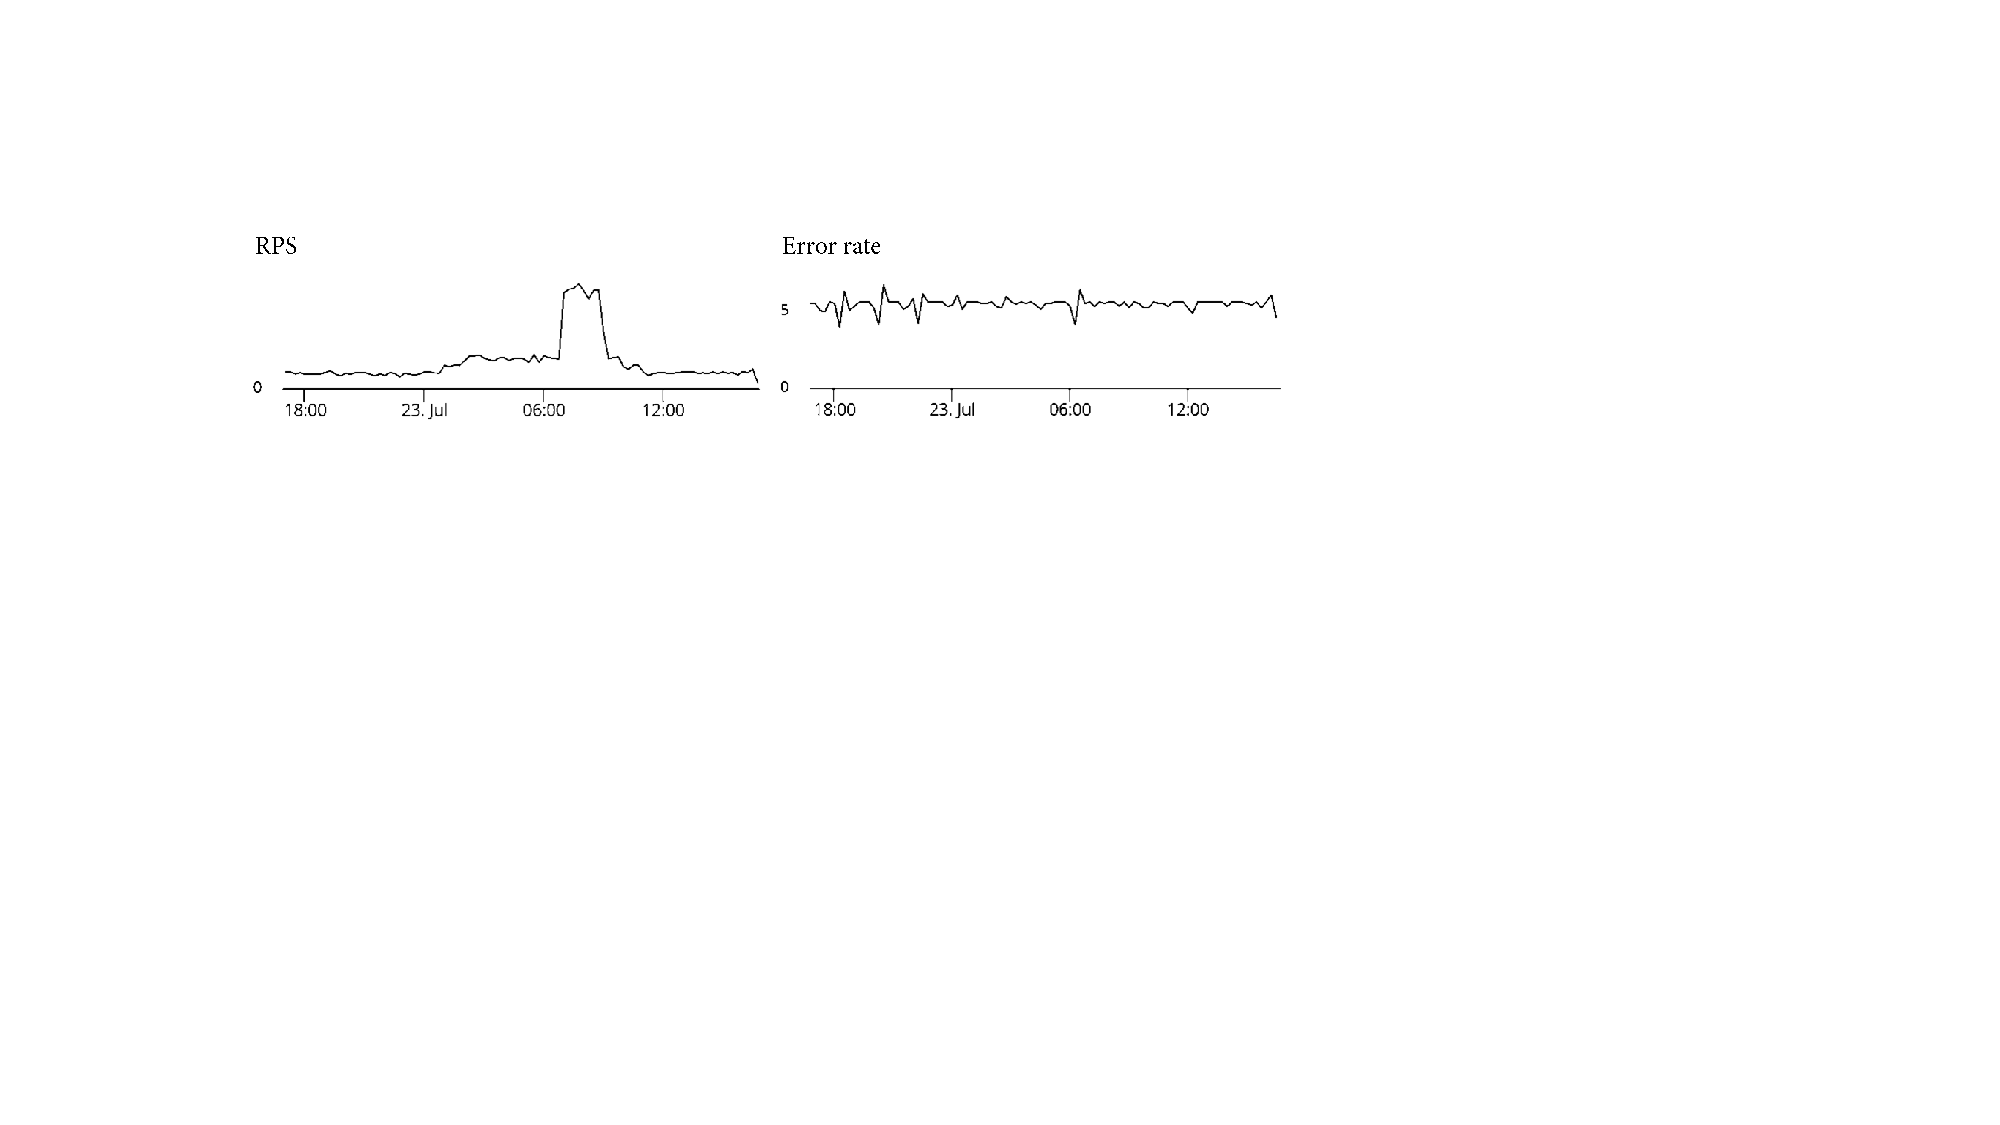
\includegraphics[width=1.0\textwidth]{gfx/chap2/rpsanderror.pdf}}
\caption{Examples of metric time series data. Response time (left) and error rate (right)~\cite{appoptics}.}
\label{fig:rpsanderror}
\end{figure}

We define a single observation of a metric as a value, timestamp, and sometimes list of properties that describe the observation, such as a source or tags. A time series is a set of observations $x_i$, each being recorded at specified time $t$~\cite{brockwell1991time}. We show examples of two time series from metric data in Figure~\ref{fig:rpsanderror}, requests per second and error rate. As metrics are simply numbers measured over intervals of time, they can be compressed, stored, processed, and retrieved efficiently. Metrics are optimized for storage and enable a longer retention of data, which can be used to build dashboards to reflect historical trends. The cost of metrics does not increase with the user traffic or any other system activity. Metrics, once collected, are more suitable for mathematical and statistical transformations such as sampling, aggregation, summarization, and correlation, which makes them better suited for monitoring and profiling purposes. Metrics are also suited to trigger alerts, as running queries against an in-memory time-series database is considerably more efficient than running a query against a distributed system storage, and then aggregating the results before deciding if an alert needs to be triggered~\cite{sridharan2018distributed,donut}.

Metrics can be sufficient for understanding the health of individual system components and application services. However, they are not sufficient to understand the lifetime of a request that traverses multiple systems, nor the semantics of the anomaly. Complex anomalies that propagate through several services and system components are more challenging to detect using solely metric data owing to the diminishing effect ~\cite{sridharan2018distributed,observability2020practical}.

\subsection{Logs} \label{ch:background:sec:observability:subsec:logs}
Logs are important in understanding and improving software systems. System operators and developers leverage the rich information in logs to generate workload information for capacity planning in large-scale systems~\cite{hassan2008industrial,nagappan2009efficiently}, monitor the overall system health~\cite{jiang2013automated}, perform anomaly detection~\cite{meng2019loganomaly,nedelkoski2019anomaly,nedelkoski2020loganomaly,nedelkoski2020selfsupervised,du2017deeplog,zhang2019robust,du2016spell,zhu2019tools}, analyze the root cause of a problem~\cite{Yuan2019AnAT,zhou2019latent,chen2019empirical}, reproduce failures~\cite{zhang2017pensieve}, improve the performance, reduce the energy consumption, address security issues~\cite{zhao2016non}, reconstruct workflows~\cite{bao2019miningworkflows}, and discover bugs~\cite{mohan2018finding}.

Logs are not only beneficial for developers and operators for successfully managing the system, but are also often needed to comply with legal regulations. For example, the Sarbanes-Oxley Act of 2002 specifies that the execution of telecommunication and financial applications must be logged to help protect the general public from errors and fraudulent practices~\cite{act2002sarbanes}.

In modern distributed systems, logs provide vital insights by capturing the state of the system for each service/component~\cite{zhu2019tools}. Logs are generally instrumented as per their usability by developers. Depending on the storage rules, they are processed, aggregated, and ultimately stored in a centralized data store from where they can be analyzed. Logs can originate from the application logic code, middleware, network communications (e.g., from switches), database communication, message brokers, caches, interaction with load balancers, and communication with security and authentication modules\cite{observability2020practical}. 

% \begin{figure}[!t]
% \centerline{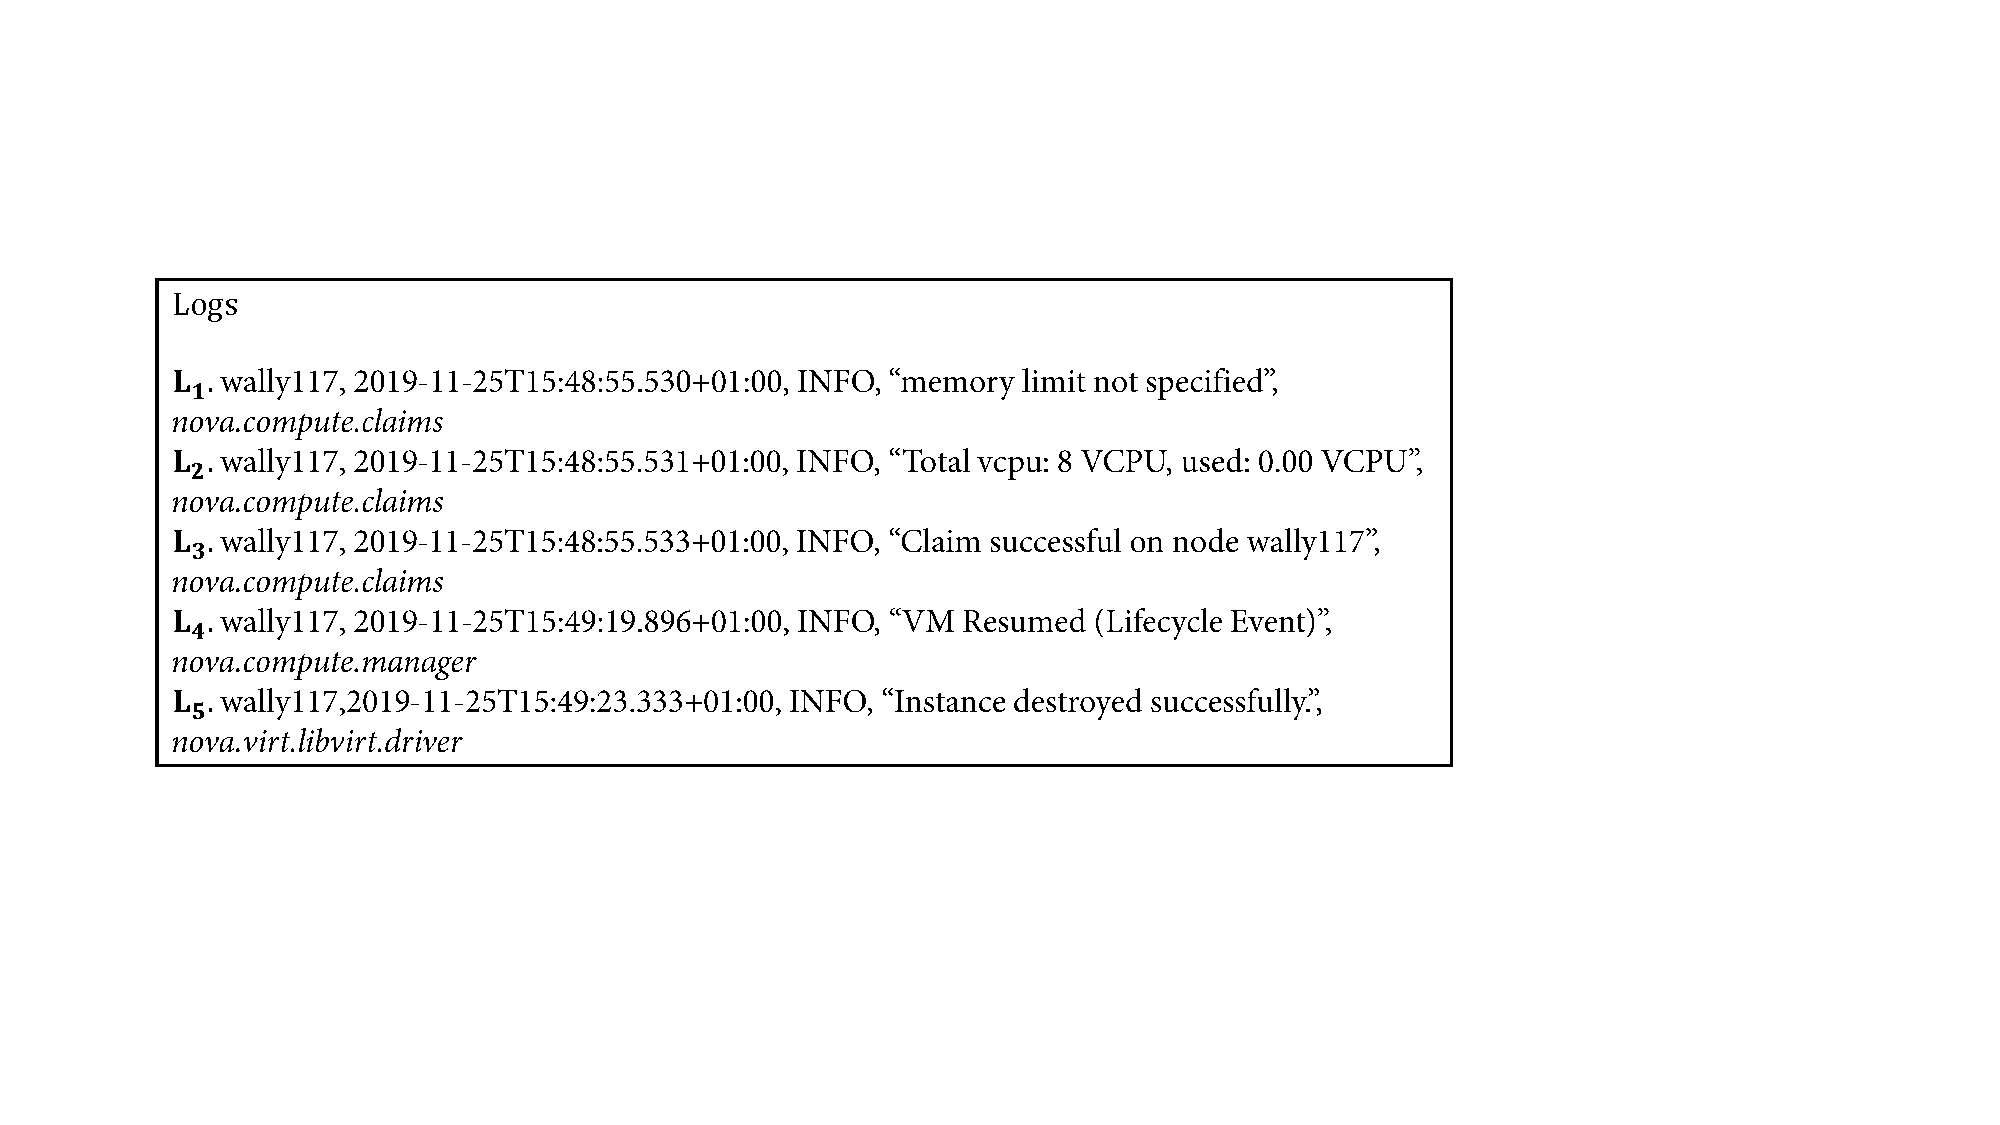
\includegraphics[width=1.0\textwidth]{gfx/chap2/log_lines.pdf}}
% \caption{Raw log messages}
% \label{fig:log_lines}
% \end{figure}

% \begin{table}[!t]
% \centering
% \caption{Raw log messages from OpenStack.}
% \resizebox{\columnwidth}{!}{%
% \begin{tabular}{l|l}
% \hline
% Nr. & \multicolumn{1}{c}{Log messages}                                                                      \\ \hline
% 1   & wally117, 2019-11-25T15:48:55.530, INFO, "memory limit not specified", nova.compute.claims            \\
% 2   & wally117, 2019-11-25T15:48:55.531, INFO, "Total vcpu: 8 VCPU, used: 0.00 VCPU", nova.compute.claims   \\
% 3   & wally117, 2019-11-25T15:48:55.533, INFO, "Claim successful on node wally117", nova.compute.claims     \\
% 4   & wally117, 2019-11-25T15:49:19.895, INFO, "VM Resumed (Lifecycle Event)", nova.compute.manager         \\
% 5   & wally117, 2019-11-25T15:49:23.333, INFO, "Instance destroyed successfully.", nova.virt.libvirt.driver \\ \hline
% \end{tabular}
% }\label{tab:log_lines}
% \end{table}

\begin{table}[!t]
\centering
\caption{Raw log messages from OpenStack cloud platform.}
\resizebox{\columnwidth}{!}{%
\begin{tabular}{cl}
\hline
Nr. & \multicolumn{1}{c}{Log messages}                                                                      \\ \hline
1   & 2019-11-25T15:48:55.530, INFO, "memory limit not specified", nova.compute.claims            \\
2   & 2019-11-25T15:48:55.531, INFO, "Total vcpu: 8 VCPU, used: 0.00 VCPU", nova.compute.claims   \\
3   & 2019-11-25T15:48:55.533, INFO, "Claim successful on node wally117", nova.compute.claims     \\
4   & 2019-11-25T15:49:19.895, INFO, "VM Resumed (Lifecycle Event)", nova.compute.manager         \\
5   & 2019-11-25T15:49:23.333, INFO, "Instance destroyed successfully.", nova.virt.libvirt.driver \\ \hline
\end{tabular}
}\label{tab:log_lines}
\end{table}

Independent on their origin type, logs contain free-form text with a timestamp, alongside other system-dependent fields. We show few typical log messages from a cloud computing infrastructure software (OpenStack~\cite{openstack}) in Table~\ref{tab:log_lines}. The first field is the timestamp when the log was generated, followed by a log level (INFO, WARNING, ERROR, etc.), payload or actual print statement written by developers, and name of the service from which was generated. Logs can also contain host names and IP addresses, class names, and other features.

Log is a string, blob of JSON, or typed key-value pairs, which enables to easily represent any data in the form of a log line. Most languages, application frameworks, and libraries are accompanied by support for logging~\cite{liu2019logzip}. Logs are also simple to instrument, as adding a log line is as trivial as adding a print statement. Logs exhibit high performances in terms of surfacing a highly granular information with a rich local context, provided that the search space is localized to events that occurred in a single service~\cite{sridharan2018distributed,hamooni2016logmine}.

However, logs, similar to the metric data, are system/service-scoped, which hinders the understanding of the full life cycle of a request that propagates through multiple connected services in the distributed system~\cite{sridharan2018distributed}. 
Often, various possible triggers across a highly interconnected graph of components are involved~\cite{gunawi2014bugs,sillito2020failures}. By solely observing discrete events that occurred in any given component at some point in time, it becomes challenging to determine all such triggers. This is the strongest drawback of log data.


\subsection{Distributed traces} \label{ch:background:sec:observability:subsec:traces}

\begin{figure}[!t]
\centerline{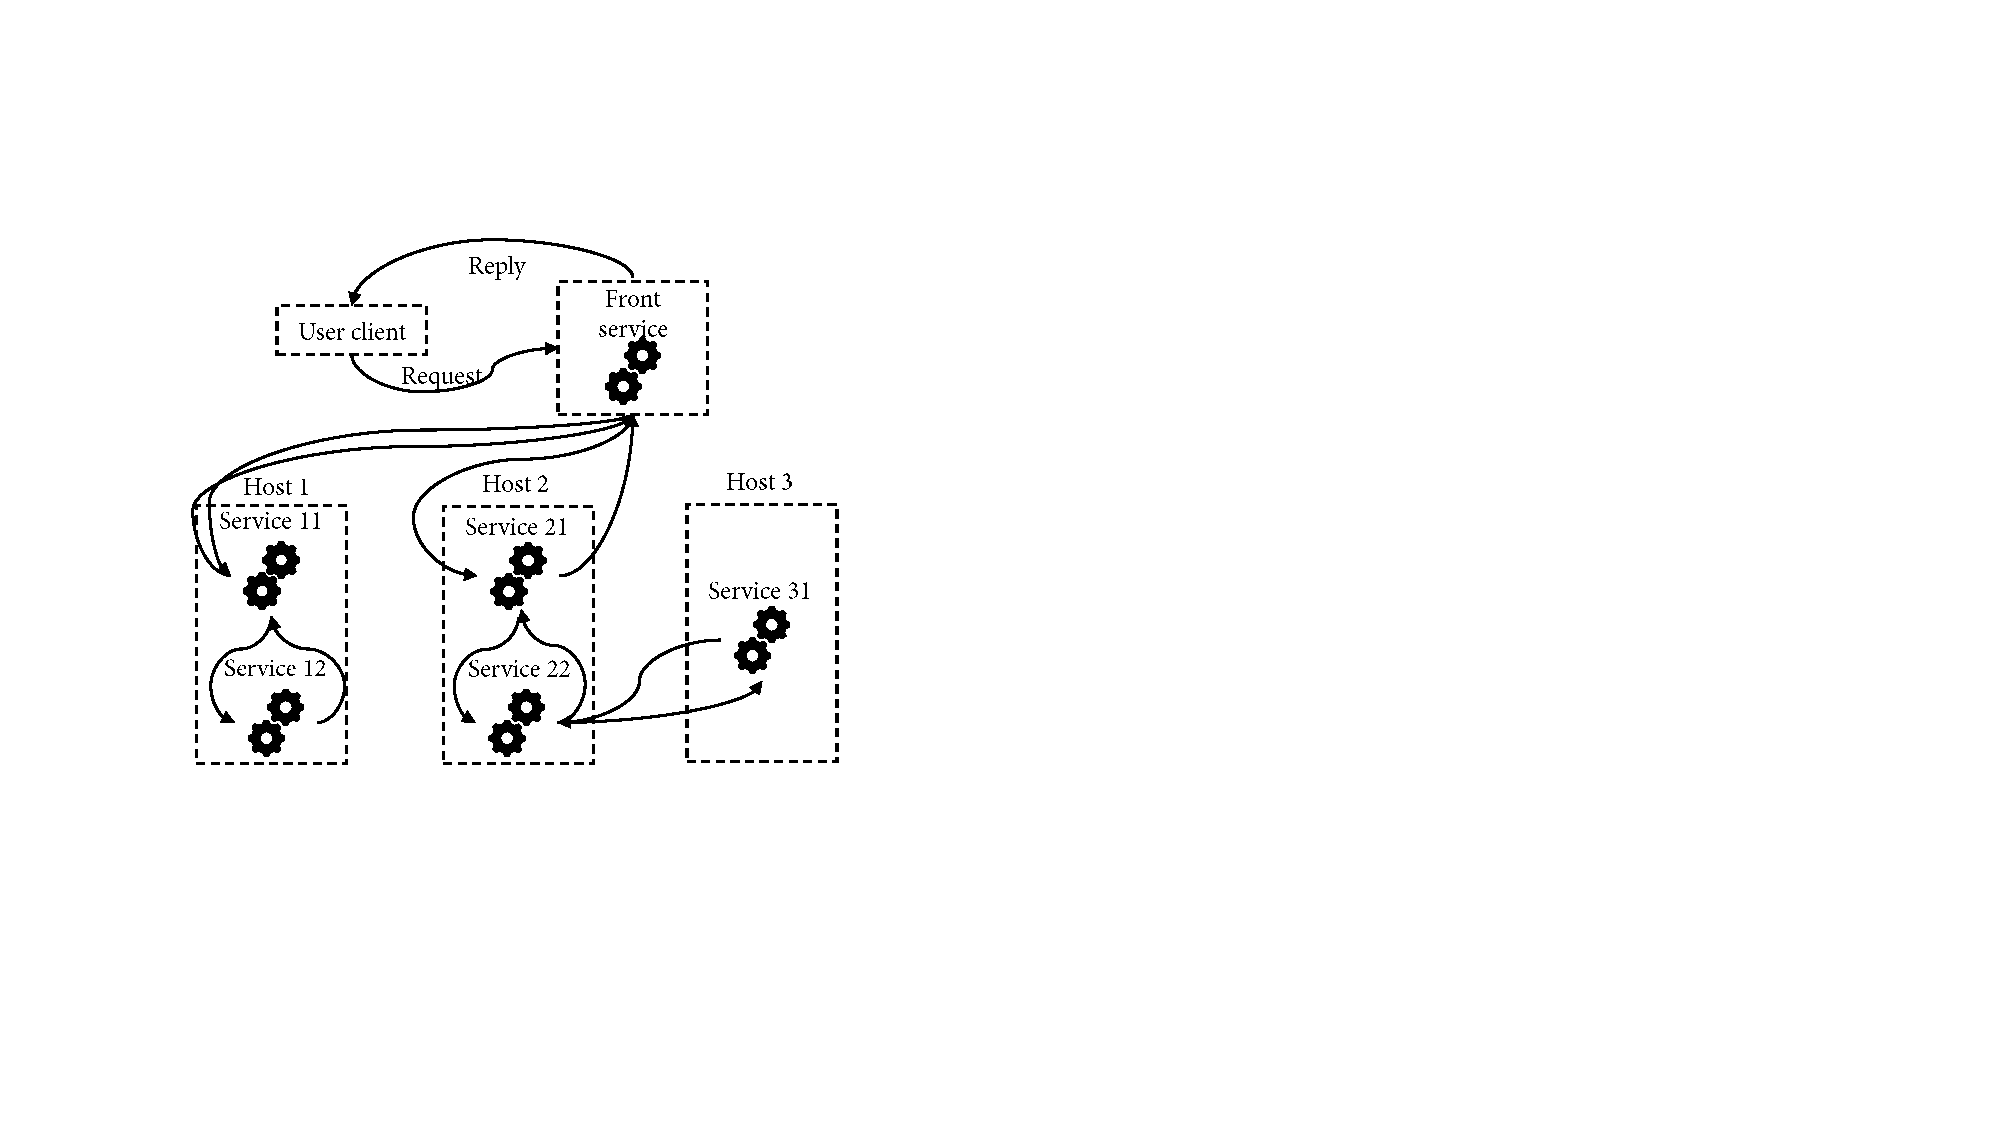
\includegraphics[width=0.8\textwidth]{gfx/chap2/pathmicroservice.pdf}}
\caption{Path through simple microservice system on behalf of the user request.}
\label{fig:pathmicroservice}
\end{figure}

The introduction of distributed traces helps address the drawbacks of the log data. They are a series of causally related distributed events that encode the end-to-end request flow through a distributed system. A single trace can provide visibility into the service response time to a request, path traversed by a request, and structure of a request~\cite{sigelman2010dapper,RepTrace}. The path of a request enables software developers and operators to understand the different services involved in executing a particular request. The structure of a request helps understand the junctures and effects of asynchrony in the execution of a request. The response time contained in the traces is related to the actual user experience, QoS, and can be considered as metric data~\cite{nedelkoski2019anomaly,nedelkoski2019anomalymultimodal}. 


A tracing infrastructure (e.g., Dapper~\cite{sigelman2010dapper}) for distributed services records information about all work in a system on behalf of a given initiator. In Figure~\ref{fig:pathmicroservice}, we show an example of a system with four servers and six microservices. We describe the path of invocation of services and simple trace. A user sends a request at the frontend. The front service sends two calls to microservices in hosts 1 and 2. Service 11 on host 1 calls service 12 (e.g., database) and responds to the request from the frontend. However, services 21 and 22 require work from service 31 at host 3, before a reply is sent to the frontend. A simple trace for this request will be a collection of message identifiers and timestamped events for every message sent and received at each service.


\begin{figure}[!t]
\centerline{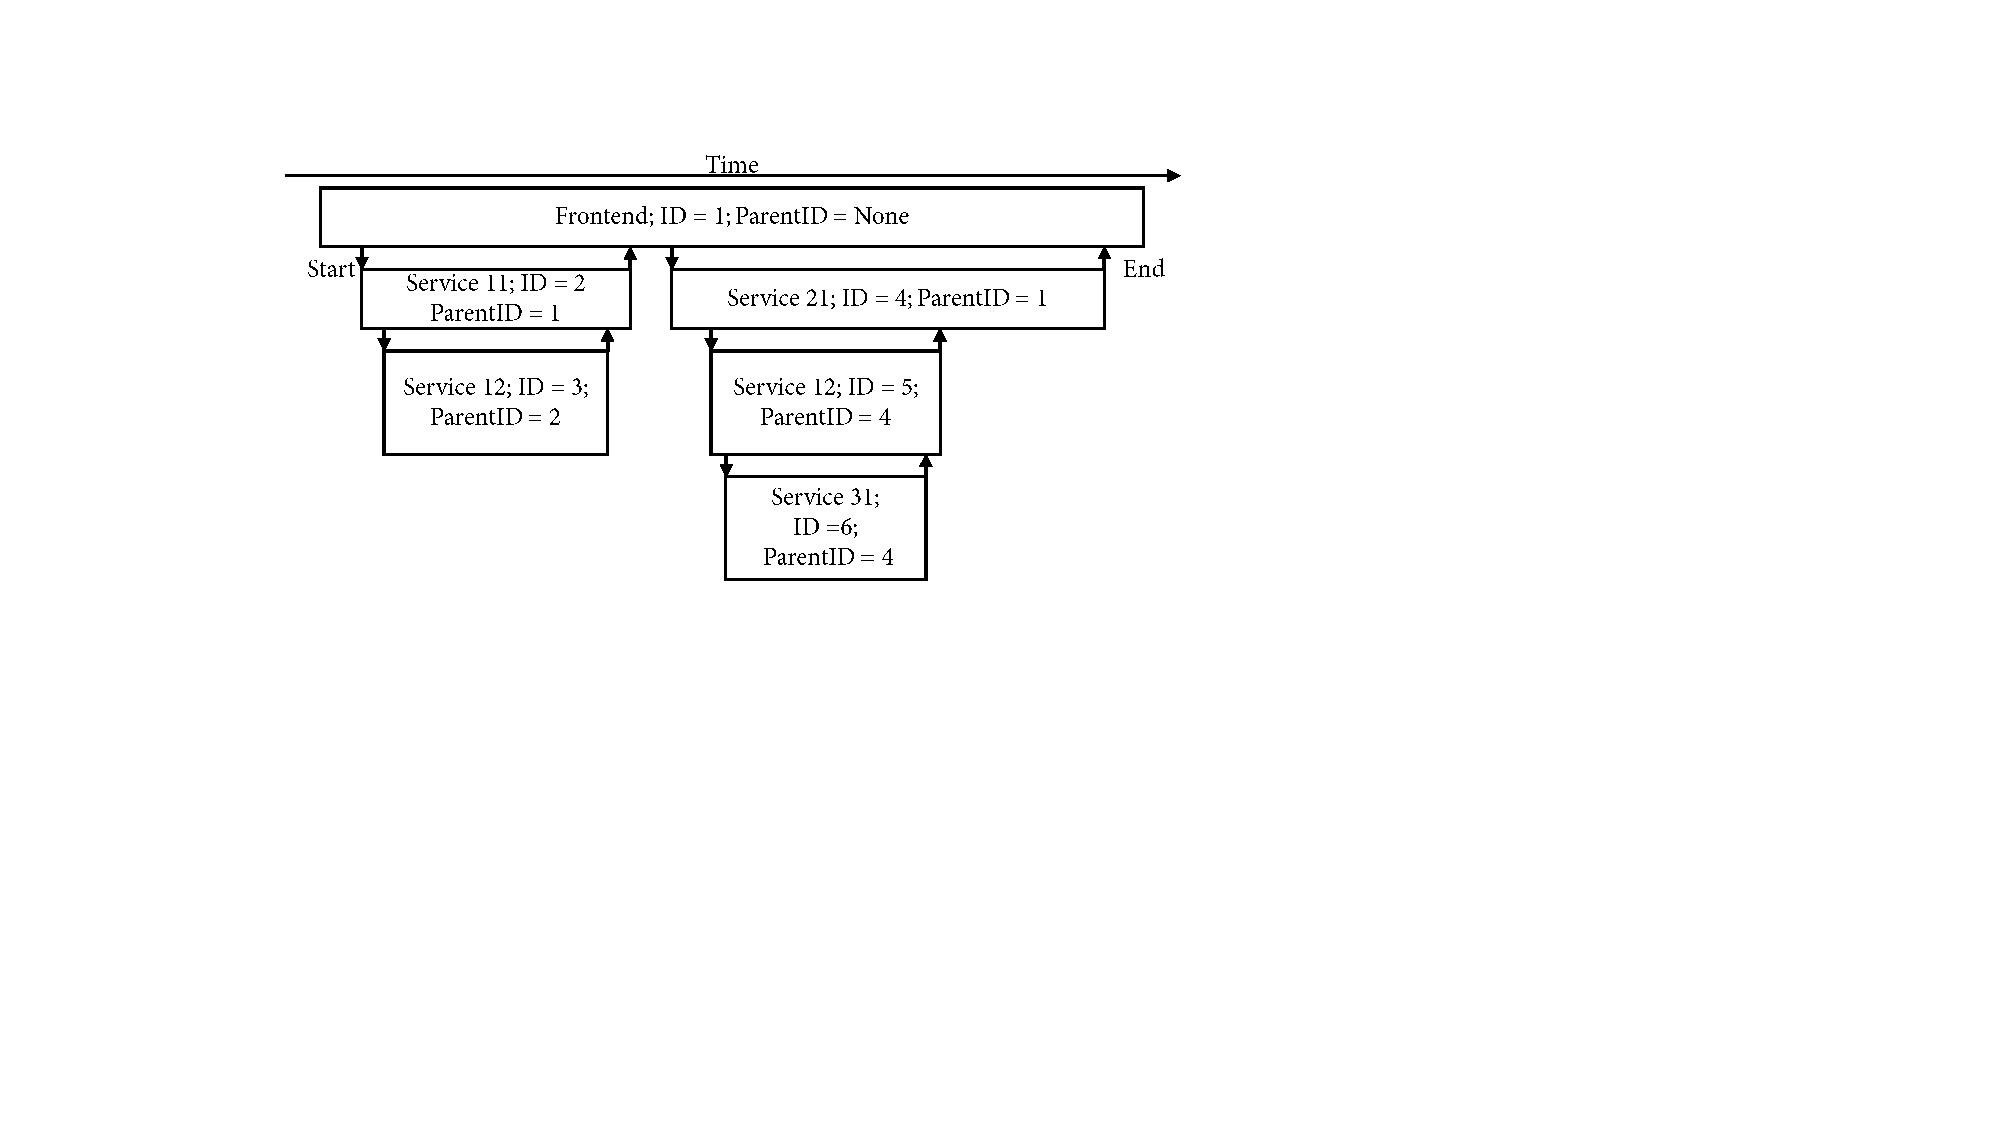
\includegraphics[width=1.0\textwidth]{gfx/chap2/tracetree.pdf}}
\caption{Causal and temporal relationships between events in a trace.}
\label{fig:temporalevents}
\end{figure}

\begin{figure}[!b]
\centerline{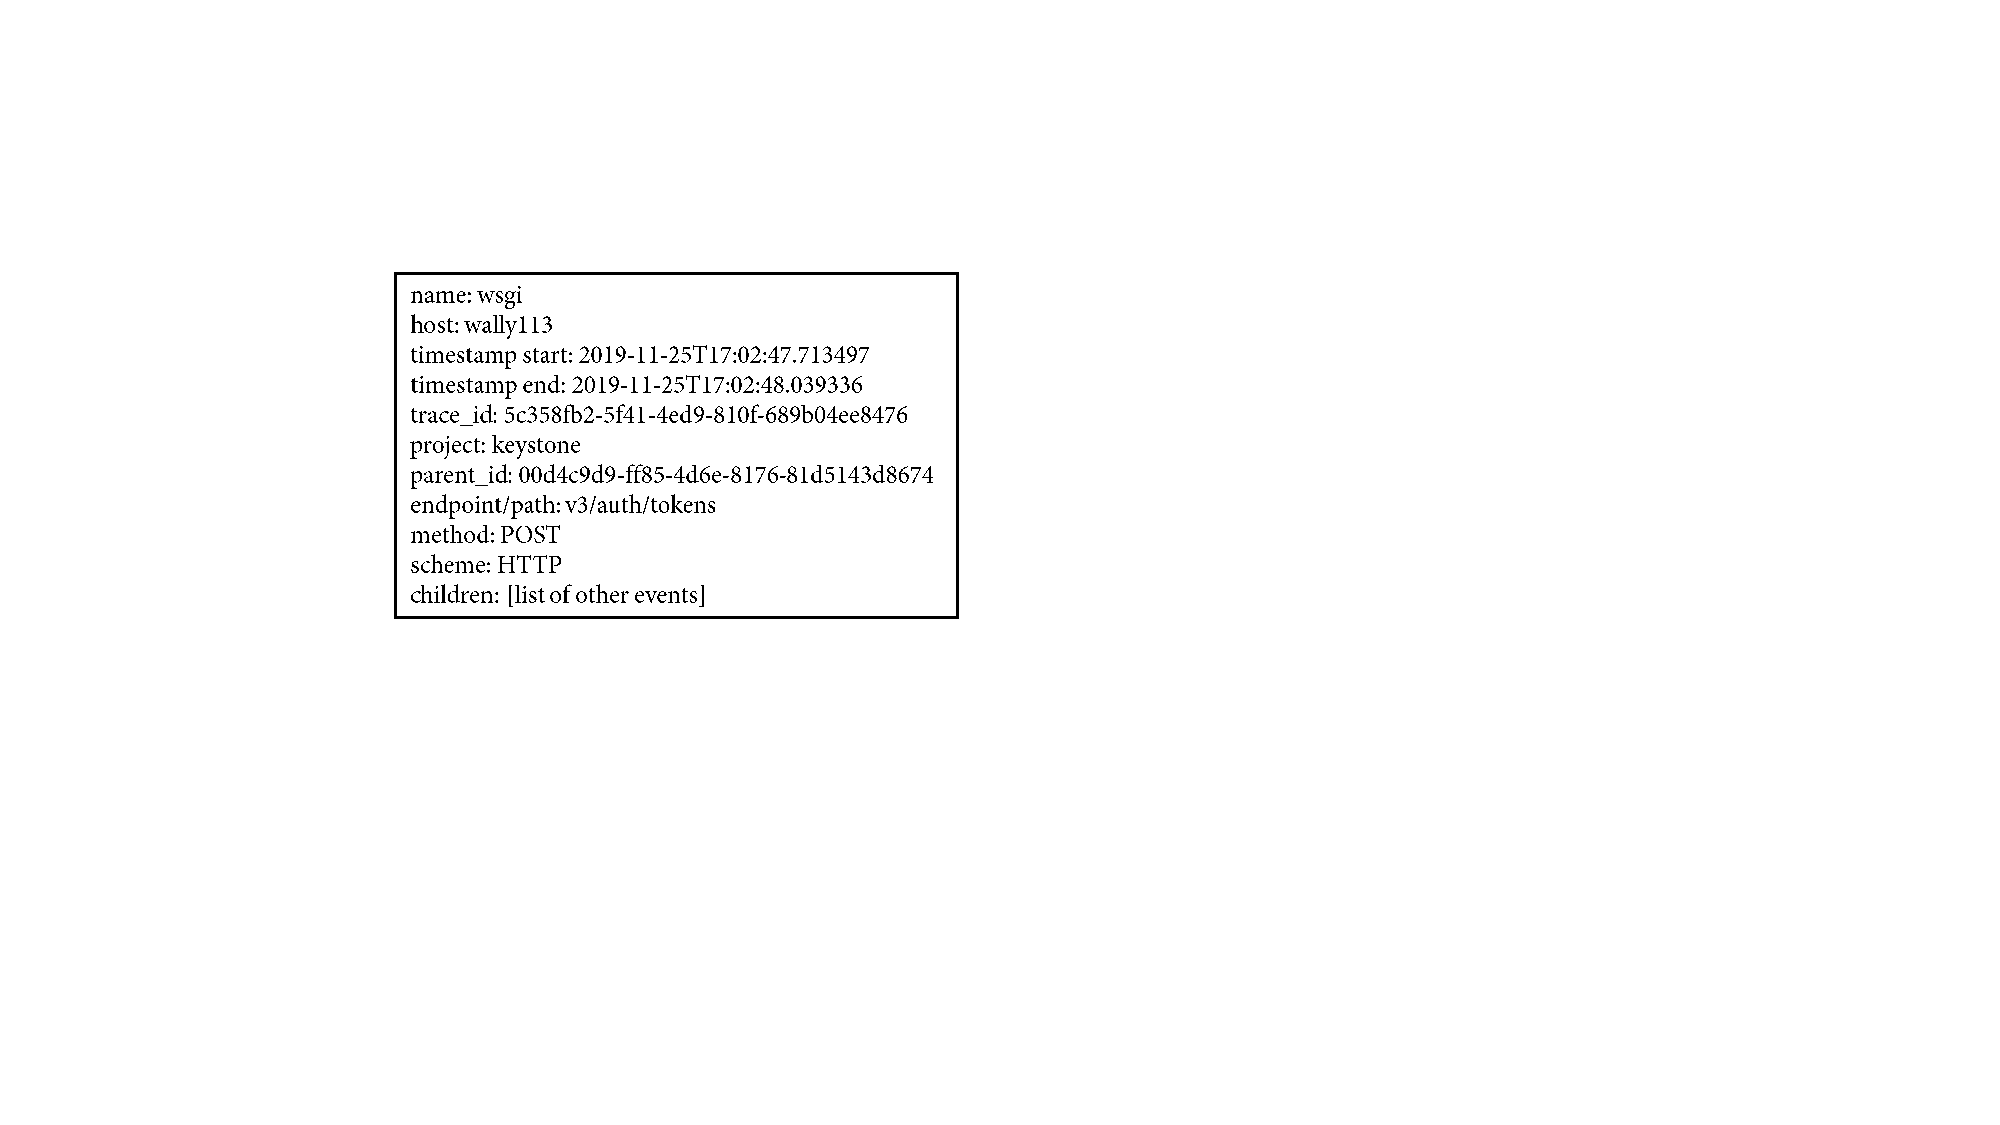
\includegraphics[width=0.6\textwidth]{gfx/chap2/single_event.pdf}}
\caption{Detailed view of a single event from a trace.}
\label{fig:singleevent}
\end{figure}


Such execution path with distributed tracing can be naturally described as a graph. In a trace graph, the nodes are basic units of work, referred to as events or spans. Each service invocation produces one span in the trace. The edges indicate a causal relationship between services. We illustrate spans forming the structure of a larger trace in Figure~\ref{fig:temporalevents}. Tracing records a human-readable span name for each span, as well as a Span ID and Parent ID. To reconstruct the causal relationships between the individual spans in a single distributed trace, we need to follow the parent--child relationship between the spans (representing a service invocation). Spans created without a Parent ID are known as root spans. All spans associated with a specific trace also share a common identifier Trace ID. All these IDs are probabilistically unique 64-bit integers~\cite{sigelman2010dapper}.

Figure~\ref{fig:singleevent} provides a more detailed view of the logged events in a typical trace span. Each span within the trace is described by its start and stop times, name of the host of the service, name of the service/project, HTTP endpoint, and list of its children spans/services. If application owners choose to augment the trace with their annotations, these are also recorded with the rest of the span data. 

\begin{figure}[!htbp]
\centerline{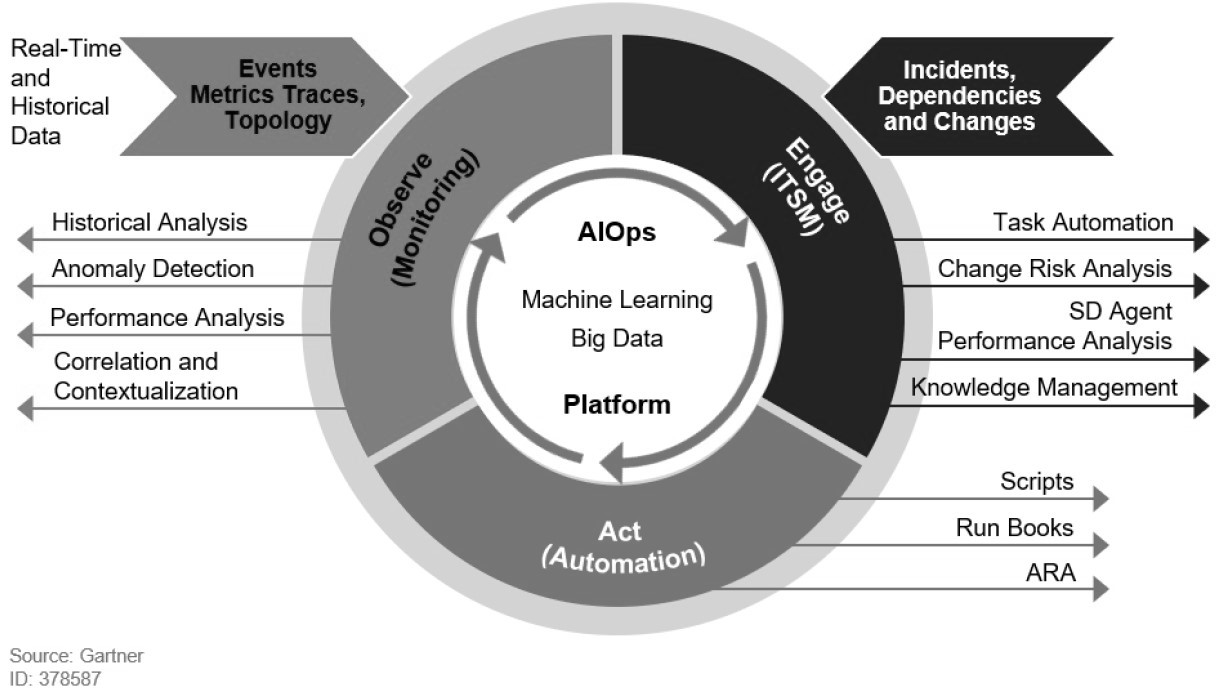
\includegraphics[width=1.0\textwidth]{gfx/chap2/aiopsgartner.jpg}}
\caption{Overview of AIOps tasks~\cite{gartnerinc,gartnermarketguide}.}
\label{fig:overviewaiops}
\end{figure}

\section{Artificial intelligence for IT systems}\label{ch:background:sec:aiops}
The amount and descriptive power of the observability data sources are favourable for the use of artificial intelligence methods. In this context, the term AIOps was coined by Gartner~\cite{gartnermarketguide} to address the DevOps challenges with AI. AIOps aims to achieve high service intelligence, customer satisfaction, and engineering productivity. However, numerous challenges still need to be overcome.





The software industry is still at the early stage of innovating and adopting AIOps solutions. According to FutureScape and Gartner predictions~\cite{futurescape2018worldwide, gartnerinc}, by 2024, 60\% of the companies will adopt ML/AI analytics for their development, maintenance, and operation tasks.

\subsection{AIOps tasks}\label{ch:background:sec:aiops:subsec:tasks}
AIOps can enhance a broad range of IT operation processes and tasks, including performance analysis, anomaly detection, event correlation and analysis, IT service management, and automation (see Figure~\ref{fig:overviewaiops}). The focus of AIOps, according to Gartner~\cite{gartnerinc,gartnermarketguide}, includes:
\begin{itemize}
    \item Basic and advanced statistical analyses: a combination of univariate and multi-variate analyses including correlations and computing other statistic indicators.
    \item Anomaly detection: use of the observed normal system behavior to initially develop a model, and then flag departures from the normal system behavior~\cite{yeanomalycloud,liu2016anomaly,vrushali2016anomaly,zhou2017anomaly}.
    \item Root cause localization: isolation of links of dependency that represent genuine causal relationships in terms of providing recipes for an effective intervention when an anomaly is detected~\cite{lou2010mining,fraenkel2004root,dalal2013empirical,nedelkoski2020rca,meng2020localizing}.
    \item Prescriptive advice and healing: classification of anomalies and root causes into known categories, relating them with solutions, analyzing the possible solutions for applicability, and offering them in a prioritized form for usage of remediation~\cite{sidiroglou2009assure,dashofy2002towards}.
    \item Topology: for the patterns detected to be relevant and actionable, a context must be placed around them. The context is topology. Without the context, the detected patterns, although valid, may be unhelpful and even distracting. Deriving patterns from data within a topology will reduce the number of patterns, establish relevancy, and illustrate hidden dependencies. Using topology as a part of the causality determination can largely increase its accuracy and effectiveness. Capturing where events occurred and their up- and downstream dependencies using graph and bottleneck analyses can provide valuable insights to focus the remediation efforts~\cite{donnet2005efficient,donnet2005improved,donnet2007internet, keller2007methods,muntonimining}.
\end{itemize}

\newpage

\section{Anomaly detection}\label{ch:background:sec:anomalydetection}
Anomaly detection has been a lasting yet active research field in various research domains for several decades. As an application-driven research field, numerous methods have been proposed including those in statistics, computer systems, healthcare, banking, and earth sciences~\cite{Aggarwal:2013:OA:2436823}. Anomaly detection is used as a general method for various techniques and approaches that share the aim of finding unusual observations in given data. A general widely accepted definition of anomaly has been reported by Hawkings~\cite{hawkins1980identification}:

\begin{center}
\textit{
"An outlier (anomaly) is an observation which deviates so much from
other observations as to arouse suspicions that it was generated by a
different mechanism."}
\end{center}


Predecessor definitions have also been reported (e.g., that by Grubbs in 1969~\cite{grubbs1969procedures}):

\begin{center}\textit{ 
"An outlying observation, or "outlier" (anomaly), is one that appears to deviate markedly from other members of the sample in which it occurs."}   
\end{center}

These definitions suggest that anomaly detection is a quite old method in computer science and statistics. However, recently, the importance of anomaly detection significantly increased with the appearance of the internet, online services, big data, large computer systems, and their economical impact. Numerous online services rely on combinations of anomaly detection methods. For example, cloud platforms utilize anomaly detection to improve their resilience and reliability, fraud detection is extensively used in the banking sector, and intrusion detection tools are implemented to prevent cyber attacks. Depending on the application and context of use, the term "anomaly" is often substituted by outlier, exception, noise, abnormality, and deviation. 

A common anomaly detection approach is to define a region representing the normal behavior and declare any observation in the data that does not belong to the normal region as an anomaly. However, several properties make this apparently simple approach challenging to use~\cite{chandola2009anomaly,pang2020deep}:
\begin{itemize}
    \item Defining a model that captures every possible normal behavior is challenging as it is not possible to identify every possible normal behaviour in most applications.
    \item When anomalies are results of malicious actions, the malicious adversaries often adapt to make the anomalous observations appear as normal.
    \item In numerous domains, the normal behavior continuously evolves and a current notion of normal behavior might not be sufficiently representative in the future.
    \item The availability of labeled data for training/validation of models used by anomaly detection techniques is often a major issue.
    \item The data contain noise, which tends to be similar to the actual anomalies, and hence is challenging to distinguish and remove.
\end{itemize}

Considering the above challenges, the anomaly detection problem, in its most general form, is not simple. Therefore, most of the existing anomaly detection techniques solve a specific formulation of the problem, which is application-dependent. 

\begin{figure}[!t]
\centerline{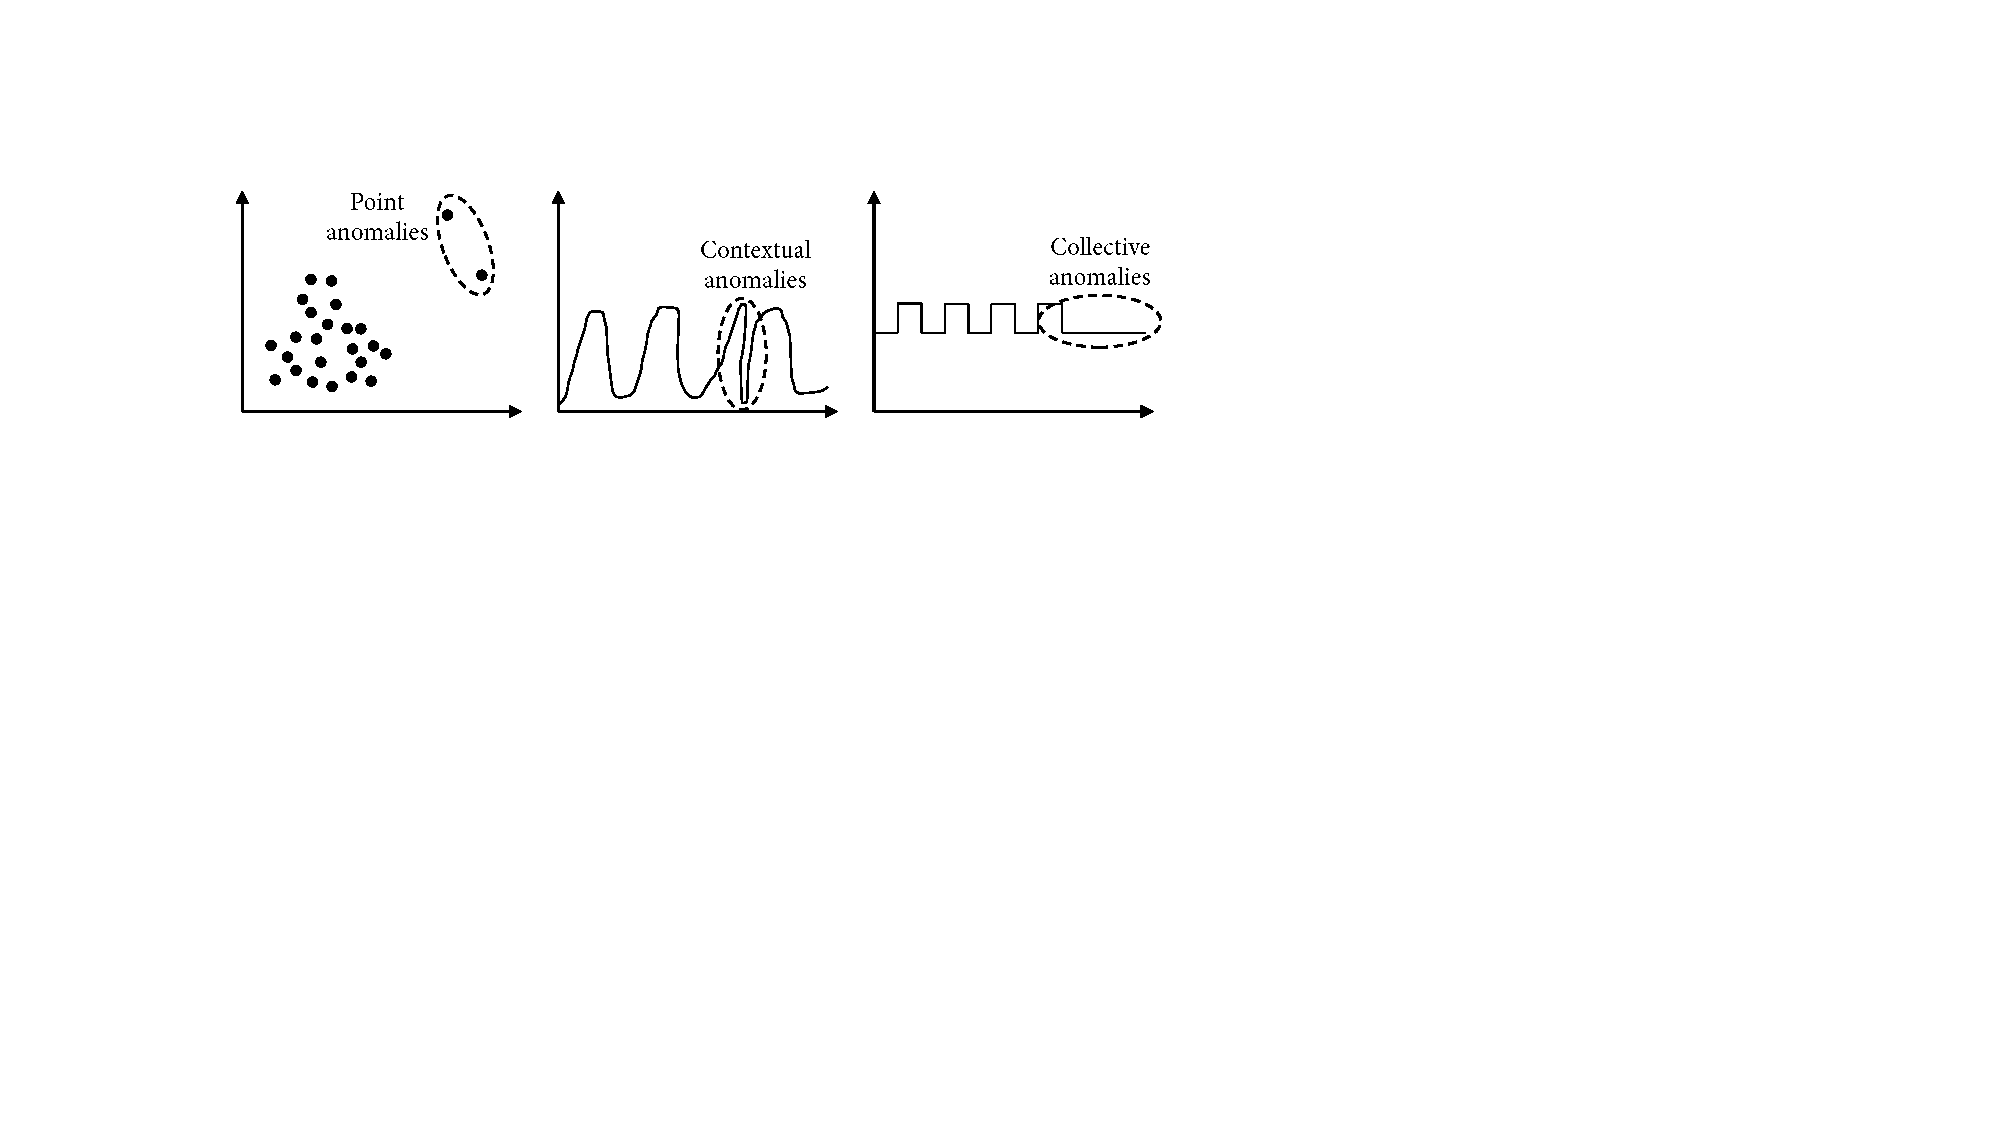
\includegraphics[width=1.0\textwidth]{gfx/chap2/typesofanomalies.pdf}}
\caption{Example of point anomalies (left). Example of a contextual anomaly (middle, the value of the data instance at the minimum is not anomalous; however, it is anomalous in the region outlined by the dashed line). Example of a collective anomaly (right); the absence of a whole group of data points forms an anomaly.}
\label{fig:typesofanomalies}
\end{figure}

Furthermore, anomalies appear in numerous different forms and contexts. In general, regarding the type of anomalies that could possibly arise, three different types are considered~\cite{chandola2009anomaly} (Figure~\ref{fig:typesofanomalies}):
\begin{itemize}
%Give examples in system data
    \item \textbf{Point anomalies} are data points that appear isolated from the bulk of the data.
    \item \textbf{Contextual anomalies}, sometimes referred to as conditional anomalies, are data points whose values are anomalous only in a specific contextual relation. Contextual features might be time, location, or broader data structure.
    \item \textbf{Collective anomalies} consist of a sequence of data points that only as a group, not as individual points, can be regarded anomalous.
\end{itemize}

Point anomalies have been extensively investigated as numerous methods assume that data points are independent instances~\cite{chandola2009anomaly,gornitz2019one}. However, data points can have strong dependencies. Therefore, it is expected to handle these data points in a collective or contextual manner. For example, asynchrony logs might not have emphasized contextual dependencies, while metric and trace data are inherently dependent.

The labels associated with a data instance denote whether that instance is normal or anomalous. Notably, the acquisition of labeled data that are accurate as well as representative of all types of behaviors is often prohibitively costly~\cite{chandola2009anomaly}. The labeling in all domains is often carried out manually by a human expert and hence a substantial effort is required to obtain the labeled training data set. Typically, the provision of a labeled set of anomalous data instances that cover all possible types of anomalous behavior is more challenging than the provision of labels for the normal behavior. Moreover, the anomalous behavior is often dynamic in nature; e.g., new types of anomalies may arise, for which no labeled training data exist. In certain cases (e.g., in air traffic safety), anomalous instances may translate to catastrophic events, and hence are rare~\cite{ruff2020unifying}. The provision of labeled data from distributed systems is costly and challenging owing to mostly practical limitations. As already mentioned, such systems undergo constant changes, e.g., software updates and hardware modernization, where labeled data become deprecated over time. Moreover, injection of anomalies to obtain data points is not possible as most running systems cannot risk possible downtimes~\cite{gunawi2014bugs,meng2019loganomaly,sillito2020failures}. Based on the extent to which the labels are available, anomaly detection techniques can operate in one of the following three modes: supervised, semi-supervised, and unsupervised anomaly detection, discussed below.

\subsection{Supervised anomaly detection} 
\label{ch:background:sec:anomalydetection:subsec:supervised}
The methods for supervised anomaly detection are similar to building predictive models~\cite{chandola2009anomaly}. These techniques assume the availability of a training data set, which has labeled instances for normal as well as anomaly classes. A typical approach in such cases is to develop a predictive model for binary classification, which aims to learn the distinctions between the normal and anomaly classes.
Any unseen data instance is compared against the model to determine which class it belongs to. 

Two major issues exist in supervised anomaly detection. First, issues emerge owing to imbalanced class distributions. Second, the provision of accurate and representative labels, particularly for the anomaly class, is usually challenging~\cite{theiler2003resampling, steinwart2005classification}. 

\subsection{Semi-supervised anomaly detection}
\label{ch:background:sec:anomalydetection:subsec:semisupervised}
In numerous real-world applications including anomaly detection in distributed systems, the operators have access to some verified (i.e., labeled) normal or anomalous samples in addition to the unlabeled data. The inclusion of these samples together with the bulk of unlabeled data leads to a semi-supervised anomaly detection problem. 

Considering $N$ (mostly normal but possibly containing some anomalous samples) unlabeled samples $x_1,\dots, x_N$ and $M$ labeled samples $(\hat{x_1}, \hat{y_1}),\dots,(\hat{x_M}, \hat{y_M})$, where $\hat{y} = 0$ and $\hat{y} = 1$ denote normal and anomalous samples, respectively, the task is to learn a model that compactly characterizes the normal class. The typical approach used in semi-supervised techniques is to develop a model for the class corresponding to the normal behavior and use the model to identify anomalies in the test data. The term semi-supervised anomaly detection has been used to describe two different anomaly detection settings. Most existing semi-supervised AD methods are instances of learning from positive (i.e., normal) and unlabeled examples. A few studies have been carried out on the general semi-supervised AD setting where labeled anomalies are also utilized. However, existing deep approaches are domain- or data-type-specific~\cite{ruff2019deep,chandola2009anomaly}. A limited set of anomaly detection techniques assume availability of only the anomaly instances for training due to the challenges to obtain anomalies that cover all cases~\cite{ruff2019deep}.

\subsection{Unsupervised anomaly detection}
\label{ch:background:sec:anomalydetection:subsec:unsupervised}
Techniques that operate in the unsupervised mode do not require labeled training data, and thus are most widely applicable~\cite{ruff2020unifying,ruff2019deep,ruff-etal-2019-self,nedelkoski2019anomaly,nedelkoski2019anomalymultimodal,nedelkoski2020loganomaly,meng2019loganomaly}. The techniques in this category use the implicit assumption that normal instances are far more frequent than anomalies in the test data~\cite{ruff2020unifying}. If this assumption is not true, such techniques suffer from a high false alarm rate. Numerous semi-supervised techniques can be adapted to operate in an unsupervised mode using a sample of the unlabeled data set as training data. Such adaptation assumes that the test data contains few anomalies. The model learnt during the training is robust to these few anomalies. However, a large gap exists between the supervised and unsupervised anomaly detection methods. The supervised anomaly detection is largely favored  under the assumption that all data are labeled~\cite{ruff2020unifying}.

\subsection{Deep anomaly detection}
\label{ch:background:sec:anomalydetection:subsec:deepanomaly}
The performances of traditional algorithms in detecting outliers can still be improved on the sequence and image datasets as they cannot capture complex patterns in the data~\cite{pang2020deep}. Moreover, as the volume of data increases, for example, to gigabytes, it becomes almost impossible for the traditional methods to scale to such large-scale data to find anomalies~\cite{chalapathy2019deep}.
To mitigate these issues, deep learning for anomaly detection, shortly \emph{deep anomaly detection}, aims to learn feature representations or anomaly scores through neural networks. A large number of deep anomaly detection methods have been introduced, with significantly higher performances than those of the conventional anomaly detection methods~\cite{pang2020deep}. However, the lack of a well-defined representative normal boundary poses challenges for both conventional and deep learning-based algorithms.

Deep neural networks leverage complex compositions of linear/nonlinear functions that can be represented by a computational graph to learn expressive representations~\cite{Goodfellow-et-al-2016}. The basic building blocks of deep learning are activation functions and layers. Activation functions determine the output of computational graph nodes (i.e., neurons in neural networks) for given inputs. They can be linear or nonlinear functions. Popular activation functions include linear, sigmoid, tanh, rectified linear unit (ReLU), and its variants. A layer in neural networks refers to a set of neurons stacked in some forms. Commonly used layers include fully connected, convolutional \& pooling, and recurrent layers. These layers can be leveraged to build different popular neural networks. For example, multi-layer perceptron (MLP) networks are composed of fully connected layers, convolutional neural networks (CNNs) have varying groups of convolutional \& pooling layers, and recurrent neural networks (RNNs), e.g., vanilla RNN, gated recurrent units (GRUs), and long-short-term memory (LSTM), are based on recurrent layers. We refer the reader to Goodfellow et al.~\cite{Goodfellow-et-al-2016} for a detailed description of the neural networks.

For a dataset $\mathcal{X} =\{\mathbf{x_1}, \mathbf{x_2}, \cdots, \mathbf{x_N}\}$ with $\mathbf{x_i} \in \mathbb{R}^{D}$ and $\mathcal{Z} \in \mathbb{R}^{K}$ as a representation space, deep anomaly detection aims to learn a feature representation mapping function $\phi(\cdot): \mathcal{X} \mapsto \mathcal{Z}$ or anomaly score learning function $\tau(\cdot):\mathcal{X} \mapsto \mathbb{R}$ in a manner that anomalies can be easily differentiated from the normal data instances in the $\phi$ or $\tau$ space, where $\phi$ and $\tau$ are a neural-network-enabled mapping function with $H \in \mathbb{N}$ hidden layers and their weight matrices $\Theta=\{\mathbf{M}^{1}, \mathbf{M}^{2}, \cdots, \mathbf{M}^{H}\}$, respectively. In the case of learning the feature mapping $\phi(\cdot)$, an additional step is required to calculate the anomaly score of each data instance in the new representation space, while $\tau(\cdot)$ can directly infer the anomaly scores with raw data inputs. 

Pang et al.~\cite{pang2020deep} provided an exhaustive overview of deep anomaly detection methods grouped by three conceptual paradigms: deep learning for feature extraction, learning feature representations of normality, and end-to-end anomaly score learning. We discuss below the main concepts and methods for each group. For details, we refer the reader to more comprehensive reviews of the literature~\cite{pang2020deep,chalapathy2019deep,ruff2020unifying}.

\subsubsection{Deep learning for feature extraction}
\label{ch:background:sec:anomalydetection:subsec:deepanomaly:subsubsecfeature}
This category of studies aims to leverage deep learning to extract low-dimensional feature representations from high-dimensional data for downstream anomaly detection. The feature extraction and anomaly scoring are fully disjointed and independent on each other. Thus, the deep learning components are used only for dimensionality reduction. Formally, the approach can be represented by

\begin{equation}\label{eqn:featureextraction}
\centering
\mathbf{z} = \phi(\mathbf{x}; \Theta),
\end{equation}

where $\phi:\mathcal{X} \mapsto \mathcal{Z}$ is a deep-neural-network-based feature mapping function, with $\mathcal{X}\in \mathbb{R}^{D}$, $\mathcal{Z} \in \mathbb{R}^{K}$, and normally $D \gg K$. An anomaly scoring method $f$ that has no connection to the feature mapping $\phi$ is then applied onto the new space to calculate anomaly scores.

Compared to the dimension reduction methods, popular for anomaly detection, such as principal component analysis (PCA)~\cite{jolliffe2016principal}, deep learning techniques have exhibited substantially better capabilities in extracting semantic-rich features and nonlinear feature relations~\cite{bengio2013representation,Goodfellow-et-al-2016}.

\subsubsection{Learning feature representations of normality}\label{ch:background:sec:anomalydetection:subsec:deepanomaly:featuresrepresentations}
The deep anomaly detection methods in this category couple feature learning with anomaly scoring to some extent, which are different from the methods in the last section, which fully decouple these two modules. 

This category of methods learn the representations of data instances by optimizing a generic feature learning objective function that is not primarily designed for anomaly detection, but the learned representations can be still utilized for the anomaly detection as they are forced to capture some key underlying data regularities. Formally, this framework can be represented by

\begin{equation}
\{\Theta^*, \mathbf{W}^*\} = {\Theta,\ \mathbf{W}} \sum_{\xvec \in \mathcal{X}}\ell\Big(\psi\big(\phi(\mathbf{x};\Theta);\mathbf{W}\big)\Big),
s_{\mathbf{x}} = f(\mathbf{x}, \phi_{\Theta^*}, \psi_{\mathbf{W}^*}) \label{eqn:genericfeature2},
\end{equation}

where $\phi$ maps the original data onto the representation space $\mathcal{Z}$, $\psi$ parameterized by $\mathbf{W}$ is a surrogate learning task that operates on the $\mathcal{Z}$ space and is dedicated to enforce the learning of underlying data regularities, $\ell$ is a loss function relative to the underlying modeling approach, and $f$ is an anomaly scoring function that utilizes these two functions with the trained parameters $\Theta^*$ and $\mathbf{W}^*$ to calculate the anomaly score $s$. This approach includes methods driven by several perspectives, including data reconstruction, generative modeling, predictability modeling, and self-supervised classification.

\subsubsection{End-to-end anomaly score learning}
\label{ch:background:sec:anomalydetection:subsec:deepanomaly:subsubsec:anomalyscore}
This approach aims to learn scalar anomaly scores in an end-to-end manner. Compared to anomaly measure-dependent feature learning, the anomaly scoring in this type of approach is not dependent on existing anomaly measures. It has a neural network that directly learns the anomaly scores. Novel loss functions are often required to drive the anomaly scoring network. Formally, this category of methods aims to learn an end-to-end anomaly score learning network: $\tau(\cdot; \Theta):\mathcal{X} \mapsto \mathbb{R}$. The underlying framework can be represented as

\begin{gather}\label{eqn:scorelearning1}
    \Theta^* = \argmin_{\Theta} \sum_{\xvec \in \mathcal{X}} \ell\big( \tau(\mathbf{x};\Theta) \big),\\
    s_{\xvec} = \tau(\mathbf{x};\Theta^*)\label{eqn:scorelearning2}.
\end{gather}


\subsubsection{Autoencoders}\label{ch:background:sec:anomalydetection:subsec:deepanomaly:subsubsec:autoencoders}
Autoencoders are utilized as a neural architecture throughout this thesis. This type of approach aims to learn some low-dimensional feature representation space on which the given data instances can be well reconstructed. This is a widely used technique for data compression or dimension reduction~\cite{hinton2006reducing,wang2014generalized,sakurada2014anomaly}. The heuristic for using this technique in anomaly detection is that the learned feature representations are enforced to learn important regularities of the data to minimize reconstruction errors. It is challenging to reconstruct anomalies from the resulting representations, and thus they have large reconstruction errors.


\begin{figure}[!t]
\centerline{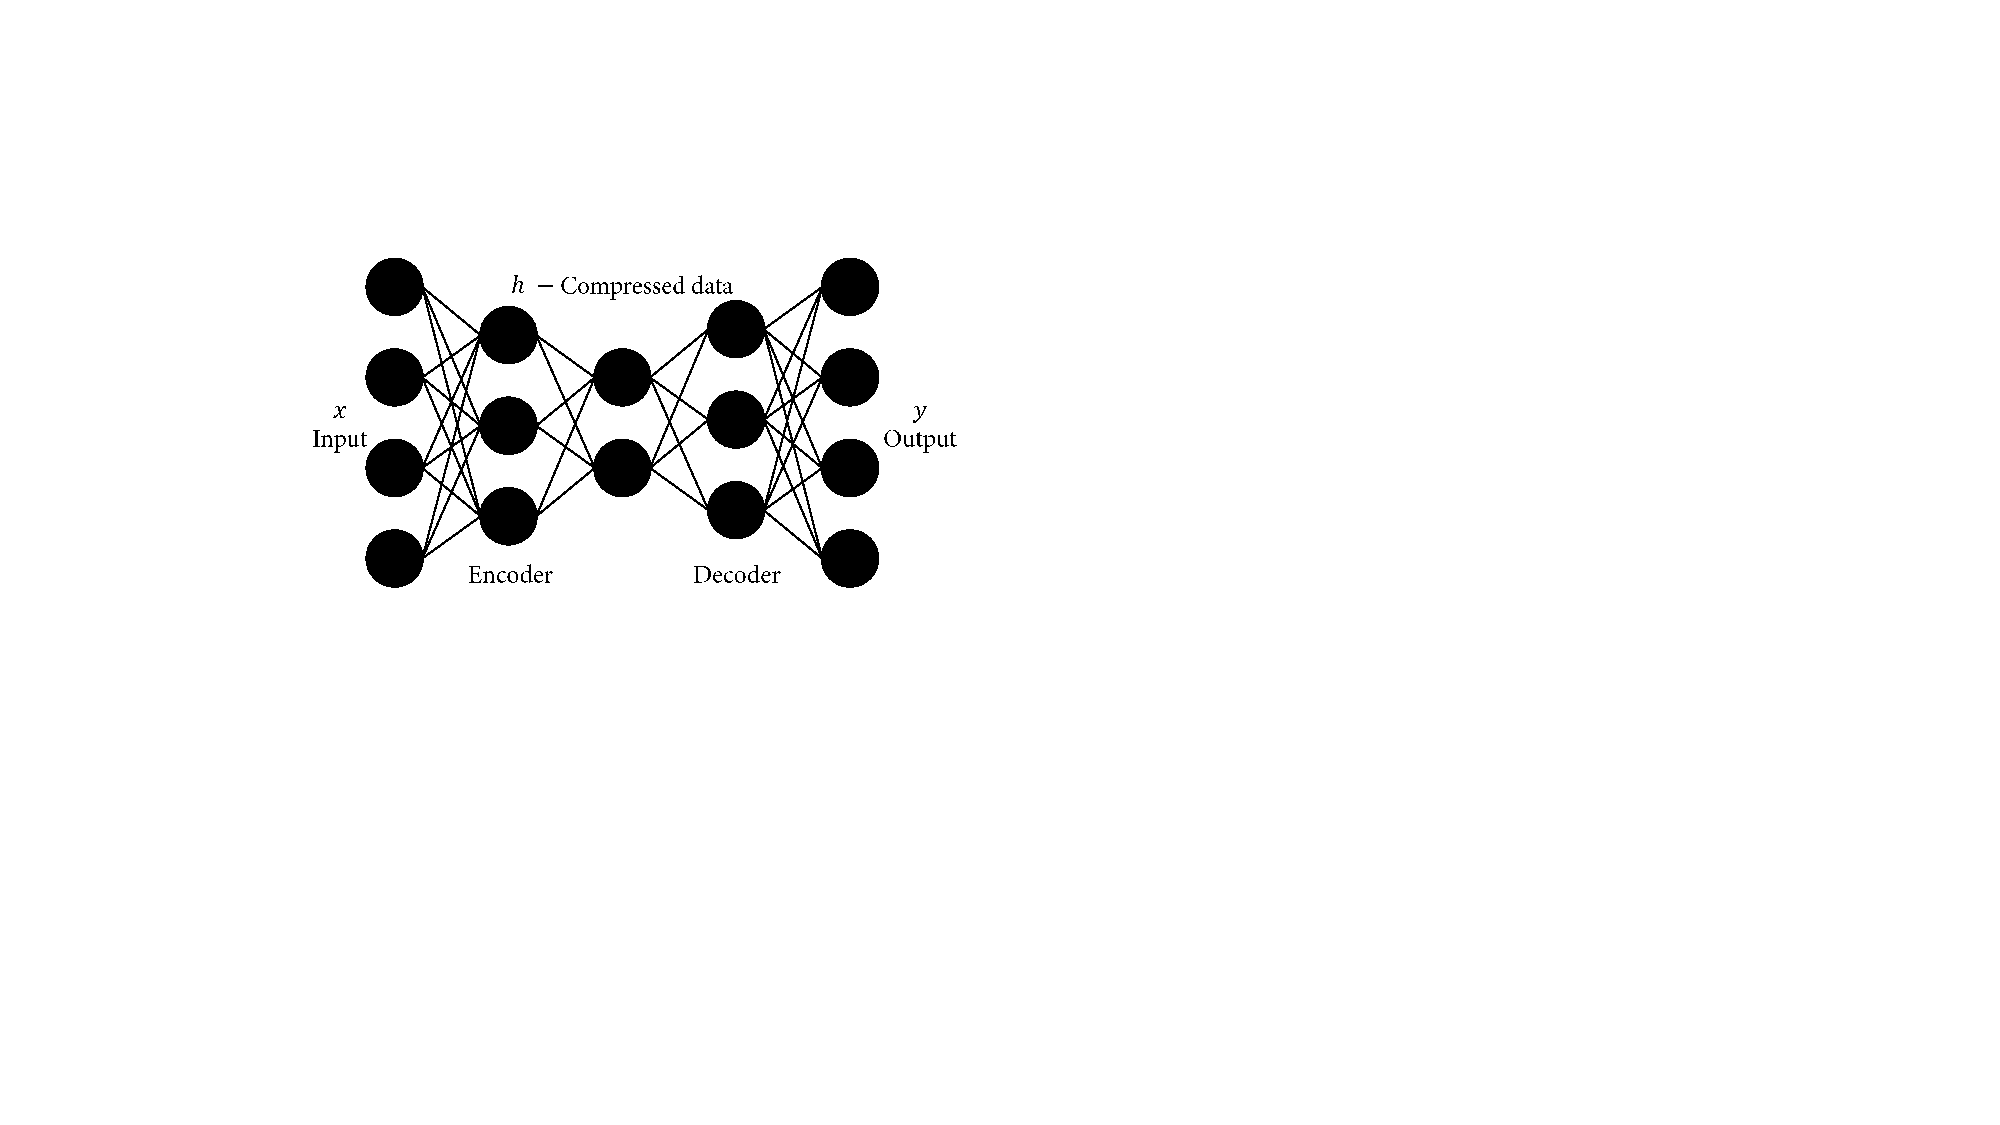
\includegraphics[scale=1.1]{gfx/chap2/autoencoder.pdf}}
\caption{Architecture of an under-complete autoencoder.}
\label{fig:autoencoder}
\end{figure}

It is assumed that normal data instances can be better restructured from the compressed feature space than anomalies. In autoencoders, the output (target) value is set equal to the input, i.e., $y_i=x_i$~\cite{hinton2006reducing} (see Figure~\ref{fig:autoencoder}). 
The autoencoder learns a function $h(w,b(x)) \simeq x$. 
In other words, it aims to learn an approximation to the identity function, to output $y$ similar to $x$.
The identity function seems a trivial function to learn. However, by placing some constraints, e.g., by limiting the number of hidden units or introducing regularization, we can extract some valuable features from the data.
Modern autoencoders have generalized the idea of encoder and decoder beyond deterministic functions to stochastic mapping.
One approach to obtain useful features, as mentioned, is to have a smaller h-dimension than x. 
This is referred to as under-complete autoencoder. Learning the under-complete representation forces the autoencoder to capture the most important features of the data. 
The learning consists simply of minimizing the error function by back-propagation.

If the hidden layer has a higher dimensionality than that of the input, the under-complete autoencoder will not learn salient features because it will only trivially copy the input to the output. A possible solution to train autoencoders is to include regularization. Rather than limiting the model capacity, regularized autoencoders use a loss function that encourages the model to have other properties besides the ability to copy its input to its output. These properties include sparsity of the representation, robustness to noise, and handling missing inputs. 
Autoencoders have been successfully applied to dimensionality reduction, anomaly detection, and information retrieval. For example, a lower-dimension representation can improve the performances of numerous tasks, such as classification, so that the models will consume less memory and run-time~\cite{ruff2020unifying,pang2020deep}.

\newpage

\subsubsection{Self-supervised learning}
\label{ch:background:sec:anomalydetection:subsec:deepanomaly:subsubsec:selfsupervised}
Self-supervised learning is learning of representations by solving auxiliary tasks. These auxiliary prediction tasks do not require ground-truth labels for learning and thus can be applied to unlabeled data, which makes the self-supervised learning suitable for anomaly detection.
Self-supervised methods introduced for visual anomaly detection train multi-class classification models based on pseudo-labels that correspond to various geometric transformations (e.g., flips, translations, and rotations)~\cite{hendrycks2019using}.
In a broader context, it is of interest to identify to what extent the self-supervision can facilitate the learning of semantic representations.
It has been evidenced that self-supervised learning helps improve the detection of semantic anomalies and thus exhibits inductive biases toward semantic representations~\cite{ahmed2019detecting}.
On the other hand, the self-supervision mainly improves the learning of effective feature representations for low-level statistics~\cite{asano2020critical}.
Hence, this research question remains to be answered. It has a high potential for numerous domains where large amounts of unlabeled data are available.


\subsection{Evaluation scores for anomaly detection methods}
\label{ch:background:sec:anomalydetection:subsec:deepanomaly:subsubsec:evaluationmethods}
To compare our method to those in the previous studies, we use the standard evaluation scores from the literature~\cite{ruff2020unifying, pang2020deep}. We evaluate our method in terms of F1-score, precision, recall, and accuracy, which depend on the true negative (TN), true positive (TP), false negative (FN), and false positive (FP) predictions. The positive class of 1 is assumed to be anomalous. The F1 score can be interpreted as a weighted average of the precision and recall. The best F1, precision, recall, and accuracy scores are 1, while the worst are 0. The relative contributions of the precision and recall to the F1 score are equal. The precision is the ratio $\frac{TP}{(TP + FP)}$, which, intuitively, is the ability of the classifier to not label as positive a sample that is negative. The recall is the ratio $\frac{TP}{(TP + FN)}$, which, intuitively, is the ability of the classifier to find all positive samples.

Even if a sufficient number of labeled samples are available, the class balances will be extremely skewed and some measures, e.g., the classification error, will not be suited to appropriately reflect the state of the generalization error. To circumvent these problems, error measures that are transient to class imbalances are used, such as the area under the receiver operating characteristic curve (AUC or AUROC)~\cite{campos2016evaluation}. The area under the
ROC curve represents the fraction of detected anomalies, averaged over the full range of decision thresholds.

 % Chapter 2
% Chapter 3
\chapter{Challenges and overview}\label{ch:concepts} 
\minitoc% Creating an actual minitoc
\bigskip

This chapter describes the main challenges, problems addressed, and assumptions made in this thesis related to anomaly detection in each of the system data sources. We position the methods developed in this thesis in the more general AIOps platform and provide an overview of the solution.

\section{Anomaly detection challenges in distributed software systems}
\label{ch:concepts:sec:anomalydetectionindistributedsoftwaresystems}
Several challenges that hinder the anomaly detection include training a model to capture every possible normal behavior, existence of anomalies from malicious adversaries, evolving normal behaviour, absence of labeled data, and high noise. 

The complex nature of the anomaly detection problem translates some of the detection challenges to the domain of distributed software systems.

\begin{itemize}
    \item \textbf{Low prediction rate.} Anomalies are rare events. It is challenging to identify all of them. Numerous normal instances are wrongly reported as anomalies while sophisticated anomalies are missed out. Although extensive studies have been carried out~\cite{liu2008isolation,breunig2000lof}, a large number of false positives exist in real-world datasets~\cite{du2017deeplog,campos2016evaluation,ruff-etal-2019-self,ruff2019deep}. Large distributed systems such as the cloud are constantly prone to new infrastructure and software updates and varying levels of load, noise, and users~\cite{zhang2015rapid}. For example, a system upgrade often generates novel log messages, changes the "normal" metric behavior, and most likely generates a different trace~\cite{zhang2019robust,nedelkoski2020selftracing}. In this regard, the data continuously evolve and thus the current normal behaviour may be outdated in the future. This creates a challenging environment for modeling of the normal behavior, which is crucial for anomaly detection.
    \item \textbf{Anomaly detection in high-dimensional data.} Anomalies often exhibit evident abnormal characteristics in a low-dimensional space, yet become hidden and unnoticeable in a high-dimensional space. Identifying high-order, nonlinear, and heterogeneous feature interactions and couplings may be essential in high-dimensional data. It is still a major challenge for anomaly detection. In addition, it is challenging to detect anomalies from instances that may be dependent on each other, e.g., by temporal, spatial, graph-based, and other interdependency relationships~\cite{pang2020deep}. These properties are particularly valid for log and trace data in distributed systems. Logs, as text data, often are represented as high-dimensional data~\cite{mikolov2013distributed}, while traces have an inherit graph-based relationship between the spans (representing services). 
    \item \textbf{Anomaly detection in noisy data.} Numerous anomaly detection methods assume that the given labeled training data are clean, which can be highly vulnerable to noisy instances that are mistakenly labeled by the opposite class label. For example, in training data collected from a distributed system, it is often assumed that all data are normal. However, with a high probability, anomaly samples exist in the training data, which can contaminate and degrade the model performance. Therefore, the models should be robust to such unknown deviations~\cite{du2019robust}.
    \item \textbf{Detection of complex anomalies.} Current methods mainly focus on detection of anomalies from single data sources, while various applications require detection of anomalies with multiple heterogeneous data sources, e.g., multidimensional data, graph, and text data. A main challenge is that some anomalies can be detected only when considering two or more data sources~\cite{pang2020deep}. Similar anomalies exist in distributed systems. For certain anomalies, no indication of the failure exists in the logs and no considerable change in the execution path in the traces is observed when the system operates in a degradation state. 
\end{itemize} 

For all observability components in distributed software systems, the large amounts of false-positive alarms are a major obstacle for using them in real-world production environments~\cite{meng2019loganomaly}. Detection of anomalies and alerting enable a system to report when something is broken or degraded. Notifying an operator is costly. When the alerts occur too frequently, operators second-guess, skim, or even ignore incoming alerts as they classify them as false positives (alarms). Sometimes even real treats masked by the noise of alarms are ignored. Therefore, effective anomaly detection and alerting systems have good signals and low noise or low rates of false alarms.

\begin{figure}[!t]
     \centering
     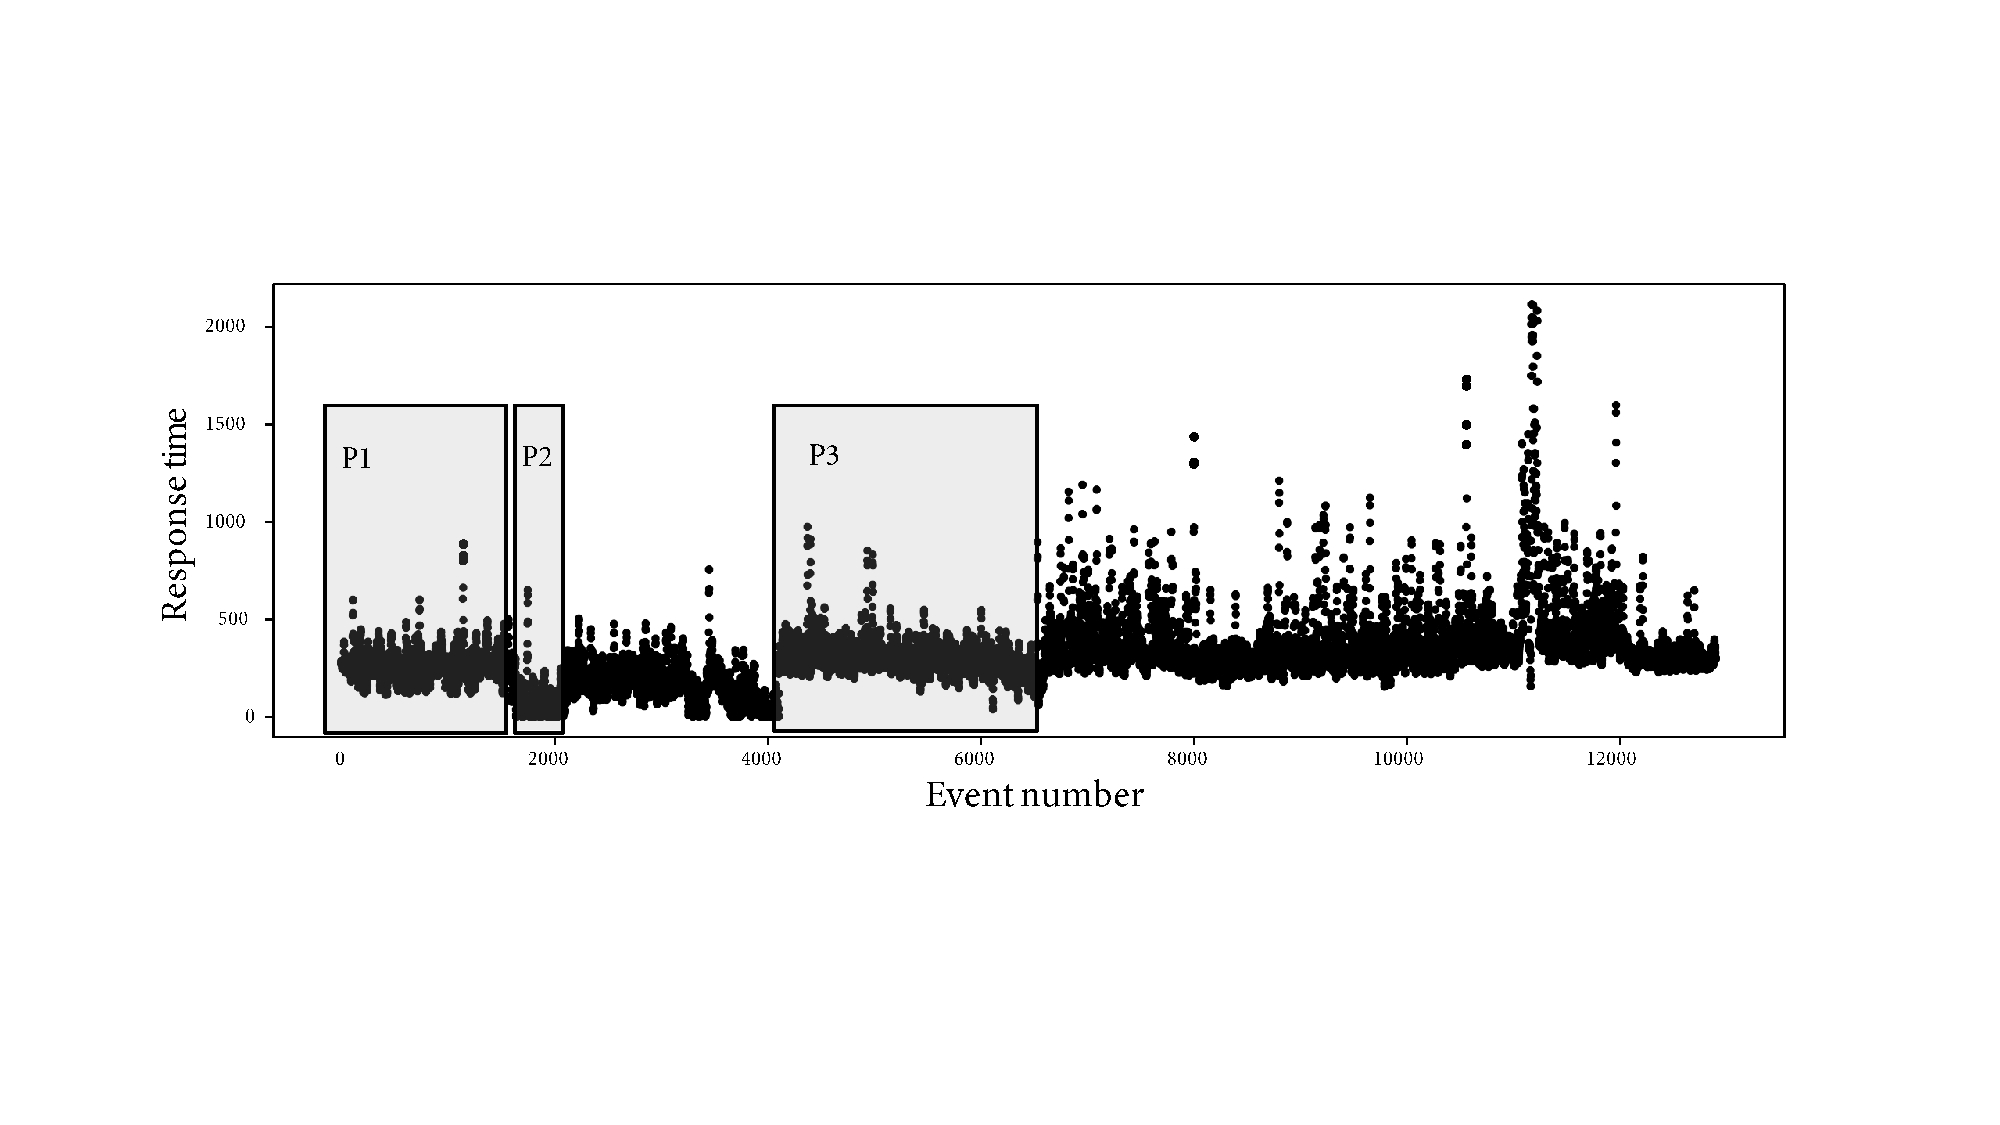
\includegraphics[width=1.0\textwidth]{gfx/chap3/multipledistributions.pdf}
     \caption{Multiple distributions representing the normal system behavior in metric data.}
     \label{fig:multipledistributions}
\end{figure}

\subsection{Metric data}
\label{ch:concepts:sec:anomalydetectionindistributedsoftwaresystems:subsec:metric}
In metric data from a distributed system, several challenges arise, including the lack of labeled data, concept drift, and concept evolution. Other major sources of difficulties emerge owing to the low signal-to-noise ratio, multiple frequencies and multiple distributions, large number of distinct time series generated by microservice applications, and concept drifts. The signal-to-noise ratio is typically low as numerous different components affect the response time of microservices such as switches, routers, memory capacity, CPU performance, programming languages, thread and process concurrency, bugs, and volume of user requests. Multiple frequencies are correlated with system and user behaviors as request patterns are different, e.g., from hour to hour due to business operation hours, from day to day due to system maintenance tasks, and from month to month due to cyclic patterns. Some of these challenges are illustrated in Figure~\ref{fig:multipledistributions}. The response time metric from a cloud service has a high level of noise ([0 ms, 2000 ms]), several distributions changing over time (P1, P2, and P3), representing the normality of the system, and additional small uptrend. 

These are stochastic properties that introduce uncertainty during the modelling phase. An additional property of metric time series inherent from time series data in general is the sequential dependence of the data points. Similar data points in the time series upon rearrangement represent different system behaviours. For example, a gradually increasing pattern, if flipped horizontally, will be a gradually decreasing pattern. The values of the data points used to form these patterns can be equal or similar; however, they reflect opposite system states. Therefore, models that aim to learn patterns from such time series need to consider the stochastic and sequential properties. 

\begin{table}[htbp]
\centering
\caption{Examples of evolving, noisy, and new log messages.}
\label{tab:evolutionlogs}
\resizebox{0.9\textwidth}{!}{%
\begin{tabular}{l|l}
\hline
Case                       & \multicolumn{1}{c}{Log messages}                                                                                                                           \\ \hline
\multirow{2}{*}{Evolution} & Faking execution of cmd: \%s"                                                                                                                              \\
                           & Faking execution of cmd (subprocess): \%s"                                                                                                                 \\ \hline
\multirow{2}{*}{Noise}     & \begin{tabular}[c]{@{}l@{}}While synchronizing instance power states, two instances \\ in the database and one instance on the hypervisor were found.\end{tabular} \\
                           & \begin{tabular}[c]{@{}l@{}}While synchronizing instance power states, two instances\\ were found in the database.\end{tabular}                                    \\ \hline
New                        & Loaded extension: binding-extended                                                                                                                         \\ \hline
\end{tabular}
}
\end{table}


\subsection{Log data}\label{ch:concepts:sec:anomalydetectionindistributedsoftwaresystems:subsec:log}
Developers and operators with understanding of the system can detect a problem that can be observed in the logs based on semantic reasoning. However, as explained above, owing to the massive amounts of log data, manual inspection is often infeasible.

In almost all live software systems, the log statements from their services evolve and are prone to processing noise over time. Developers may frequently modify source codes including logging statements, which in turn leads to changes to log data. Kabinna et al.~\cite{kabinna2018examining} observed that approximately 20\%-45\% of logging statements in their studied projects changed throughout their lifetime. Google’s systems have up to thousands of new log printing statements every month~\cite{xu2010system}. 

Furthermore, during collection, retrieval, and preprocessing of log data, a certain degree of noise is inevitably introduced into the original log data. For example, the noise may originate from the data collection process. In a large-scale system, numerous logs are produced by geographically distributed components separately, and then uploaded to a centralized location for further analysis. Missing, duplicated, or disordered log messages can originate from such a process (e.g., due to network errors, limited
system throughput, and storage issues).

We show examples of evolving, noisy, and new log statements in Table~\ref{tab:evolutionlogs}. In the case of evolving statements, the (subprocess) word is added for clarity. In the noisy logs, owing to the lack of instances on the hypervisor, a different print statement that shortens the message is observed. In system upgrades, often new log messages appear owing to, e.g., extensions. 

Logs are developer-written text sentences. Each developer has a specific style of programming and writing log statements~\cite{zhu2019tools}. This contributes to the inability of log analysis methods (e.g., parsing and anomaly detection) to have a standardized or more structured approach that will generalize across different datasets with minimal number of domain/system based heuristics.

These problems suggest that any method developed for log analysis needs to discard the close-world assumption, where systems are not evolving~\cite{du2019lifelong,du2017deeplog}. The methods need to address the described challenges during the design of their models. This is particularly important for organizations that use the Continue Delivery/Deployment approaches, where the environment poses larger challenges~\cite{chen2015continuous}.

\begin{figure}[!htbp]
     \centering
     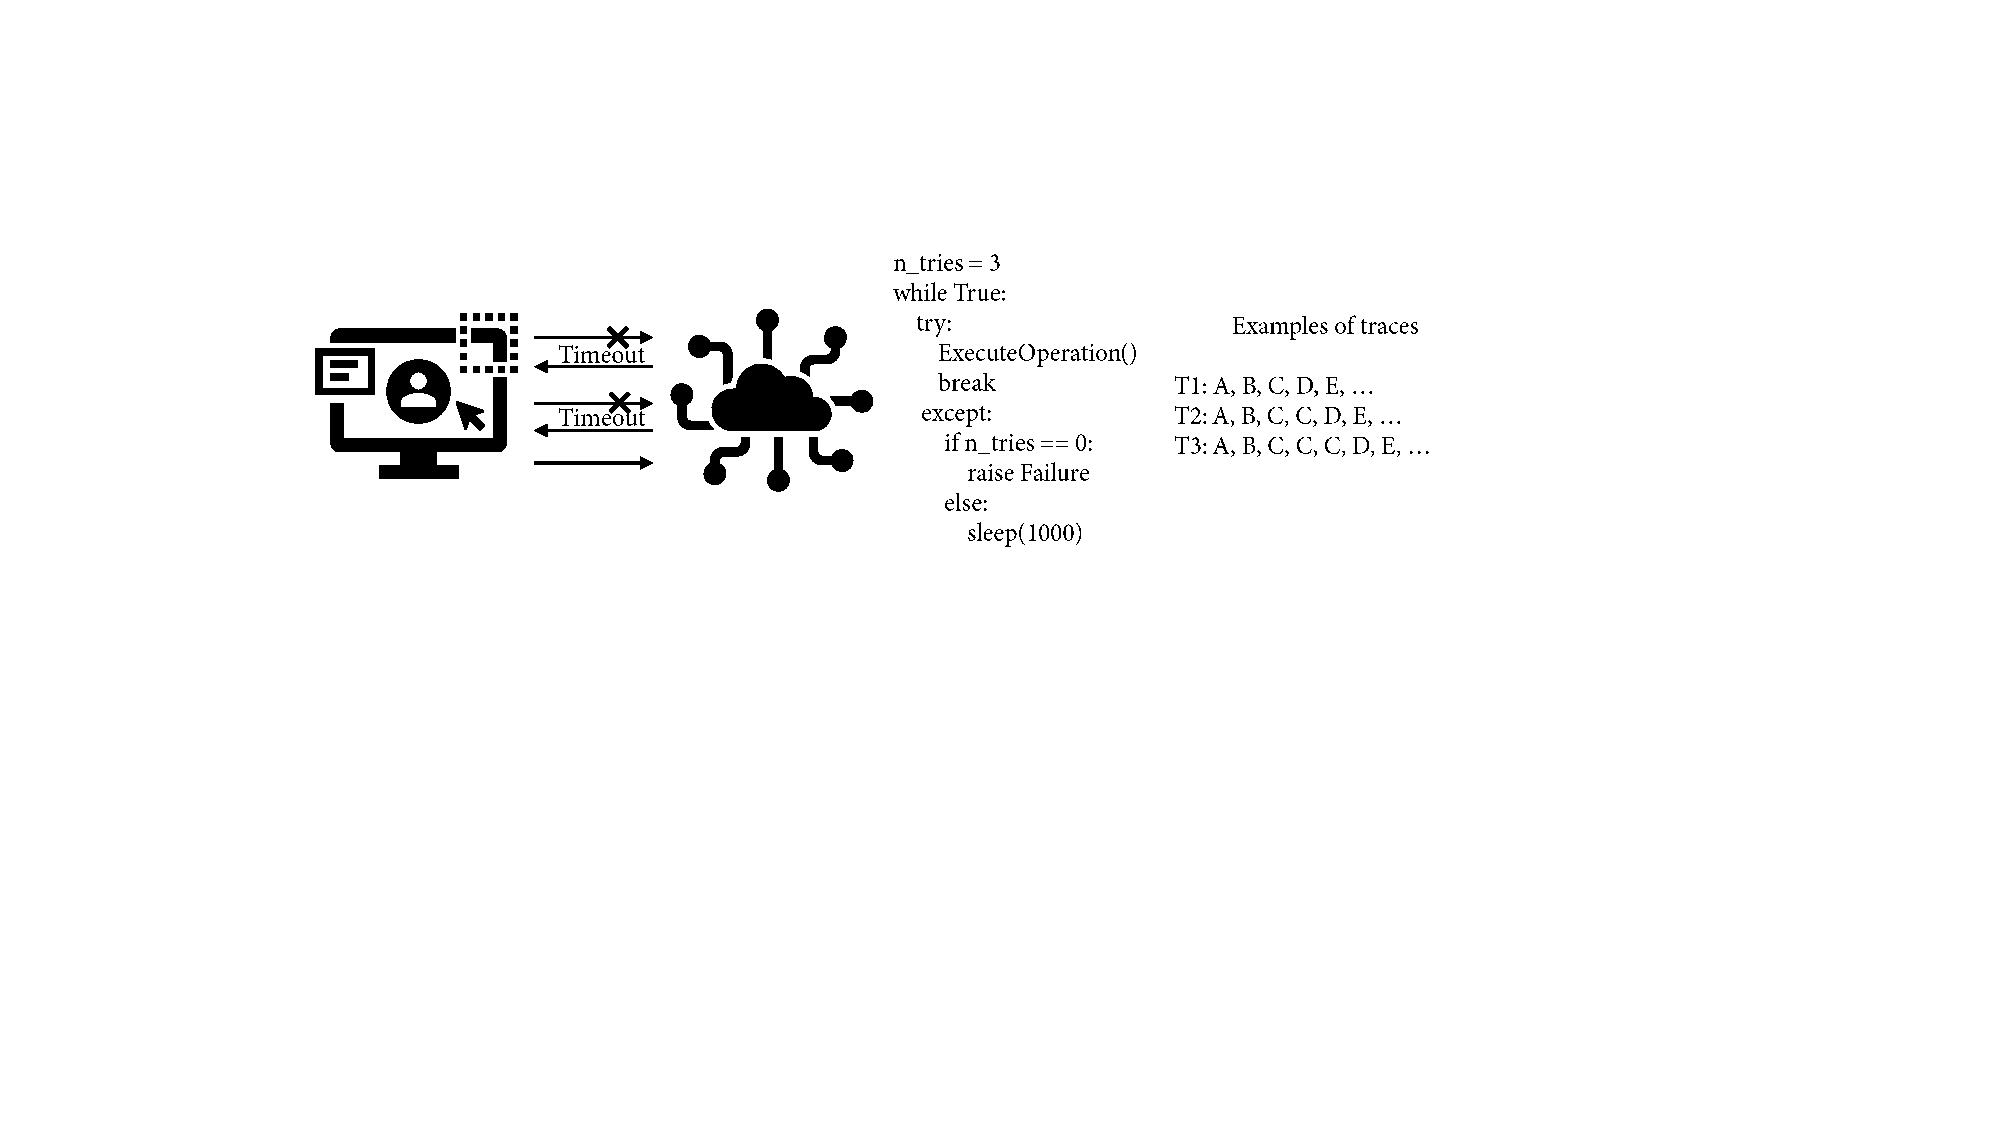
\includegraphics[width=0.99\textwidth]{gfx/chap3/traceschallenges.pdf}
     \caption{Software patterns; e.g., the retry pattern affects the running system and trace data.}
     \label{fig:tracechallenges}
\end{figure}

\subsection{Distributed tracing data}\label{ch:concepts:sec:anomalydetectionindistributedsoftwaresystems:subsec:trace}
Three important challenges exist in anomaly detection from distributed traces. They are related to the existence of noise, arbitrary lengths of the traces, and lack of labels. From these challenges, the lack of labels is a lasting problem in the task of anomaly detection in general and was described in the previous chapter.

Owing to the complex nature of the operations within a distributed environment and high noise, although the observed sequence of events may not be present in the set of observed traces, it may still be normal. Noise in the traces occurs because complex systems rely on software patterns, such as caching and load balancing, to increase the efficiency and reliability. For example, it can be a retry pattern where an operation is executed, leads to a timeout, and is performed again until completion (see Figure~\ref{fig:tracechallenges}). The noise has a strong implication for trace anomaly detection as methods need to classify traces that were not observed before as normal. 

The challenge related to the range of lengths of a trace occurs mainly owing to the existence of different requests. For example, creation of a virtual machine and creation of a storage will lead to two different traces. The novel methods for anomaly detection from distributed traces, similarly to metric and log data, are faced with the scarcity and unavailability of labels when a trace is normal or anomaly. The unsupervised learning methods are considered as obtaining labels from the systems is a challenging task. The frequent system updates and volatile environment contribute to the manifestation of new patterns, which imposes a constraint of frequent updates of the labels. This is often an expensive procedure because it assumes constant availability of a domain expert.


\subsection{Complex anomalies}\label{ch:concepts:sec:anomalydetectionindistributedsoftwaresystems:subsec:complexanomalies}
Anomalies can be complex and not always represented in all data sources. Examples of such anomalies are hidden anomalies, not reflected in all observability data, and propagated anomalies, reflected in a set of system components different than the faulty component. These anomalies may not be notified to the user through exceptions or may not be monitored~\cite{sillito2020failures}. These cases represent a high risk for system operators as they lack clues for understanding the failure and restoring the availability of services and resources~\cite{gunawi2014bugs,cotroneo2019bad,sillito2020failures}. 

According to a set of experiments~\cite{cotroneo2019bad} on OpenStack, software anomalies often cause an erratic behavior of the cloud management system, hindering detection and recovery of failures. Failures were notified to the users only after a long delay, when it is more difficult to trace back the root cause of the failure and recovery actions are more costly (e.g., reverting the database), or the failures were not notified. Anomalies are not always present in all observability components and often propagate and are detected at system components different than the root-cause component. This makes the task of debugging more challenging. Therefore, for improved diagnostics, often, a combination of highly accurate models for anomaly detection in multi-view data sources is required.

\subsection{Assumptions}
In this section, we discuss observations in each of the data components, which were treated as assumptions for the design of the practical solutions. 

\noindent\textbf{General assumptions.} Throughout this thesis and description of the methods, unless otherwise stated, we use a general assumption that all data used to create the models reflect the normal system behaviour and almost do not contain anomalies~\cite{chandola2009anomaly,ruff2020unifying,ruff2019deep}. Most of the systems operate normally, most of the time, while anomalies occur rarely~\cite{du2017deeplog,meng2019loganomaly,nedelkoski2019anomalymultimodal}. Thus, in most of the production cases, using all available data satisfies the assumption, considering that, even if anomalies are present, their number is considerably smaller than the number of normal data points. The models described in this thesis implement practices to handle such cases. 

A general assumption for most deep learning methods, also implemented in this thesis, is the existence of a sufficient amount of data representing the normal system behavior. Unless otherwise stated, anomaly labels are not accessible. These are important assumptions for the development of anomaly detection methods for distributed system data. They pose requirements for the methods to be unsupervised, which is desirable and of practical value.

Lastly, a general assumption of this thesis is that system anomalies are reflected in at least one of the three data sources. In practice, the anomaly may not be reflected in the data, but can only be found by reproduction and troubleshooting in the source code. We assume that the source code of the system is not available.

Below, we discuss assumptions considered for each of the data sources.

\begin{enumerate}
    \item \textbf{In metric data}, we assume univariate time series data (unless otherwise stated in a particular experiment). Univariate anomaly detection aims to find anomalies in each individual metric, while multivariate anomaly detection learns a single model for all metrics in the system. Univariate methods are simpler, and thus they can be more easily scaled to many metrics and large datasets~\cite{Sandilands2014}. However, the task of learning the causal relationships between the anomalies in the resulting alerts from the univariate anomaly detectors remains to be performed on a higher level of abstraction~\cite{simhon2016heuristic}. This is in line with the long-lasting research on univariate time series data~\cite{braei2020anomaly}. With multivariate methods, each added metric introduces interactions between it and all other metrics. As multivariate anomaly detection methods have to model the entire complex system, the computational cost rapidly increases with the number of modeled metrics. In addition, individual metrics need to have similar statistical behaviors for accuracy of the multivariate methods~\cite{toledano18a}.
    
    \item \textbf{Logs} are generated by a software program that follows a set of instructions to serve a request, e.g., creating a virtual machine in cloud platforms. In distributed systems, multiple such requests are served in parallel. In many systems, the logs do not contain identifiers that could chain events that serve the same requests together into a group. Often, when sorted by timestamp, such sequences of logs are lost. Therefore, in this thesis, we focus on the analysis of the collected log messages as independent instances. The log anomaly detection method detects anomalies per log message, not per sequence of log messages. 
    
    A common assumption in anomaly detection from logs is that the information of the log messages is contained in their log templates (constant parts). For example, we consider a log message "Took 20.12 seconds to build instance". The methods for log-based anomaly detection focus on detecting anomalies on "Took * seconds to build instance", without considering the variable part. This assumption is common in numerous log anomaly detection approaches ~\cite{du2017deeplog,meng2019loganomaly,zhang2019robust,du2019robust,he2017drain}. Anomalies that exist in the variable parts of the log messages (e.g., numeric values) are considered as a part of time series anomaly detection (metric data). 
    \item \textbf{For trace data}, we assume that the traces are composed of a finite number of possible spans. This implies that test traces are composed of spans observed during the modeling phase. As the spans correspond to invoked services, we consider this as a weak assumption, which is not valid only when new services are deployed. In this regard, the learned model on the traces will need to be retrained once a new service is deployed within the distributed system. 
\end{enumerate}

\section{Conceptual overview}\label{ch:concepts:sec:conceptualoverview}
To address the above challenges and consider the assumptions for anomaly detection, in this thesis, we present methods for the three observability components, metrics, logs, and traces.  
The observability and anomaly detection methods are base components of a broader-context platform referred to as AIOPs platform. We show a reference architecture in Figure~\ref{fig:aiopsplatform}, where a software system based on a distributed architecture (e.g., microservices) is deployed. 

\begin{figure}[!t]
\centerline{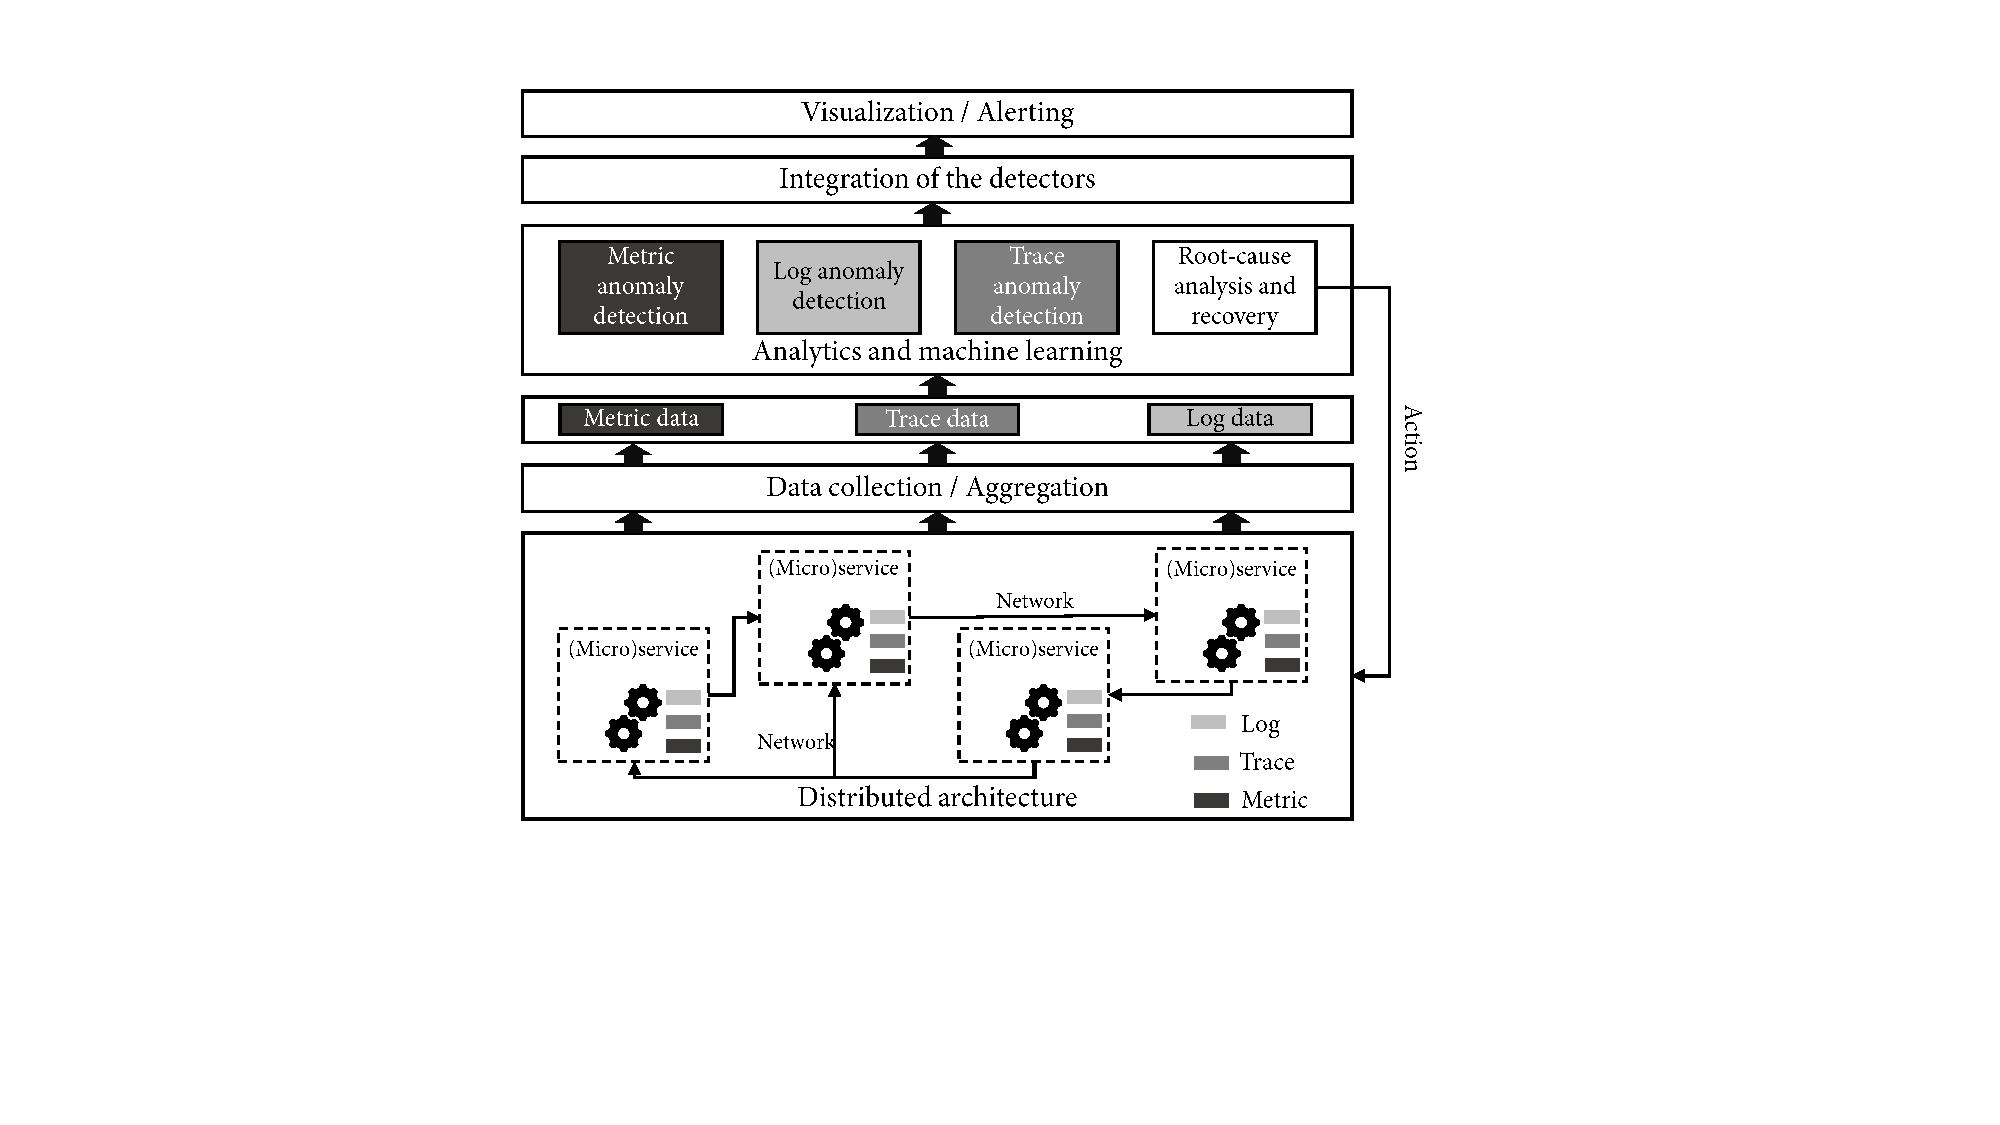
\includegraphics[scale=0.8]{gfx/chap3/aiopsplatform.pdf}}
\caption{Overall architecture of a distributed system with integrated observability components (metrics, logs, and traces) utilized by the analytic part for visualization and alerting.}
\label{fig:aiopsplatform}
\end{figure}

In every service of the distributed system, three data collection components, metrics, logs, and traces, exist. The data are then aggregated and forwarded to the analytic part. For the metric data, the aggregation is carried out per service where metrics such as CPU, memory, disk utilization, and network statistics are collected. The logs from all services are aggregated in a database with a possible separation by the service/physical host. Finally, the tracing data involve multiple hosts and services traversed while executing a request (e.g., user request). 

The data serve as a basis for the analytic and machine learning parts where several major tasks are performed. The analytic part involves preprocessing for each type of data. 

In the anomaly detection module, we consider three anomaly detectors $f_m(\mathbf{x_m})$, $f_l(\mathbf{x_l})$, and $f_t(\mathbf{x_t})$ for the metrics, logs, and traces, respectively. The input data in (1) $f_m(\mathbf{x_m})$ are a time series representing a system metric $\mathbf{x_m}={x_m^{w_m}, x_m^{w_m}, \dots, x_m^{w_m}}$, where $w_m$ is a window size, in (2) $f_l(\mathbf{x_l})$ are a system log message $\mathbf{x_l}={x_l^1, x_l^2, \dots, x_l^m}$, where $x_l^i$ are $d-$dimensional representations of the words in the log message and $m$ is the number of words, and in (3) $f_t(\mathbf{x_t})$ are a trace $\mathbf{x_t} = {x_t^1, x_t^2, \dots, x_t^k}$, where $x_t^i$ is a span and $k$ is the number of spans in the  trace. 
Each of the separate methods for anomaly detection in metrics, logs, and traces presented in this thesis is designed to mitigate the previously described challenges. Below, we present main questions derived from the challenges and methods to address them on an abstract level.

\begin{enumerate}
    \item The challenges of anomaly detection in metric data pose difficulties toward an accurate understanding of the system behavior. The major questions are related to the efficient extraction of temporal correlations within the time series, learning of multiple modes of normal behavior, noise mitigation, and description of the anomaly patterns. We address these questions aiming to improve the analysis of metric data and alert the user if there is an abnormal system behavior in the system. The core idea of the approach is to learn robust latent representations to capture normal patterns of a time series, considering both temporal dependence and stochasticity. We design the method's basis to have a variational component that provides the needed capacity of the method to learn multiple scenarios of normal system behavior and mitigate the effect of the noise and recurrent encoder and decoder networks to extract sequential features. 
    
    \item System log analysis is a lasting research topic, which, through the years, established an analysis pipeline. Traditionally, the first step in the process is to parse the unstructured log messages into structured data or extract log templates. Structured data usually refer to the constant string in each log message or the print statement. Subsequently, these templates are vectorized (e.g., count vectors~\cite{lou2010mining,xu2009detecting}) to obtain numerical representations suited for further analysis. Lastly, the log vectors are utilized as an input to the anomaly detection model. It is important that all steps in the pipeline are addressed correspondingly. Therefore, we analyze several topics including the generalization of parsing and log anomaly detection methods on unseen log messages (e.g., due to upgrades), efficient log parsing without system-dependent heuristics, and generation of learnable log vectors that are sufficiently robust to mitigate the effects of log evolution. We start with a self-supervised neural language modelling approach to log parsing. The advantage of such approach is that it replaces heuristics with learnable parameters optimized for the respective data. Concurrently, the model is designed to learn and generate log vectors, which is crucial to improve the anomaly detection~\cite{zhang2019robust}. To further improve the generalization in log anomaly detection, we describe a novel objective function and propose modification to the parsing approach. Such approach aims to learn meaningful log representations for anomaly detection, regularize against over-fitting, extract semantic knowledge from the log messages, and improve the generalization. The core principle of the method is to learn log representations in a manner to distinguish normal data from the system of interest and anomaly samples from auxiliary easily-accessible log datasets. 
    
    \item The challenges of the trace data lead to several questions, which, when addressed, have the potential to improve the anomaly detection. The research questions regarding the trace data that are addressed in this thesis are related to the modeling of traces with variable lengths, mitigation of the noise that reflects as added/missing spans form the trace, and identification of key spans within the trace, representative of the normal system behaviour, which help find the root cause of the problem. We compile the trace structure as a text sequence. This allows to utilize methods from the field of natural language processing that already tackle problems as modeling inputs with different lengths (e.g., for texts). Subsequently, to mitigate the effects of the noise, we present a task formulation based on self-supervised learning to learn the likelihood of appearance of particular span with given context spans. This enables the model to focus on particular important spans of the trace and mitigate the effects of the noise. 
\end{enumerate}

The output of each anomaly detectors at time $t$ is a label $y\in\{0,1\}$, where 0 represents a normal system behaviour, while 1 represents an anomaly.
On top of the outputs of the anomaly detection methods, a time window $w$ is utilized to aggregate the predictions for a final decision, whether an anomaly exists in the observed distributed system. Formally, the final output at a time of $t$ is $g_t(f_m, f_l, f_t, w)$, which again is 0 or 1. The main contributions of the thesis are the methods presented for metrics, logs, and traces. Finally, we analyze their integration into a framework for detection of complex anomalies.

The identified anomalies can be further employed in other AIOPs tasks. For example, together with the system topology, they are often utilized to perform a root cause analysis to identify the reason for and location of the anomaly. To complete the AIOPs loop, recovery actions need to be executed to restore a failed component or prevent further fatalities. Finally, the alerts from the anomaly detection, root cause analysis, and recovery actions are visualized to the developers, reliability engineers, and management teams to obtain better insights into the system. 
 % Chapter 3
% Chapter X

\chapter{Anomaly Detection in Metric Data} % Chapter title
\label{ch:metrics}
\minitoc
\bigskip

Anomaly detection for metric data with various
patterns and data quality has been a great challenge, especially
without labels. Existing anomaly detection algorithms suffer from the hassle of algorithm picking/parameter tuning, heavy reliance on labels, which among other challenges results in large number of false alarms. Metric time series from distributed systems exhibit complex temporal relationships and stochasticity~\cite{donut,fraccaro2016sequential}. 
Accordingly, a possible solution should address both properties. In this chapter, we present a method that captures normal patterns of a time series with an unsupervised anomaly detection model based on VAE (captures stochastic properties) with an RNN as encoder and decoder parts (captures temporal dependence). The observations that deviate from this model of normality are likely to be considered anomalies. 


We summarize the contributions in this chapter, which form a part of a metric anomaly 
10
 detection method, denoted as Metano~\footnote{Parts of this chapter are published in ~\cite{nedelkoski2019anomaly,nedelkoski2020rca,nedelkoski2019edge} and patented in~\cite{nedelkoski2020patent}.}.
\begin{itemize}
\item Model for metric anomaly detection in metric data.
\item Dynamic error threshold approach coupled with a tolerance module to reduce the FP predictions.
\item Anomaly classification module to enrich the description of the anomaly patterns.
\end{itemize}


\begin{figure}[htbp]
\centerline{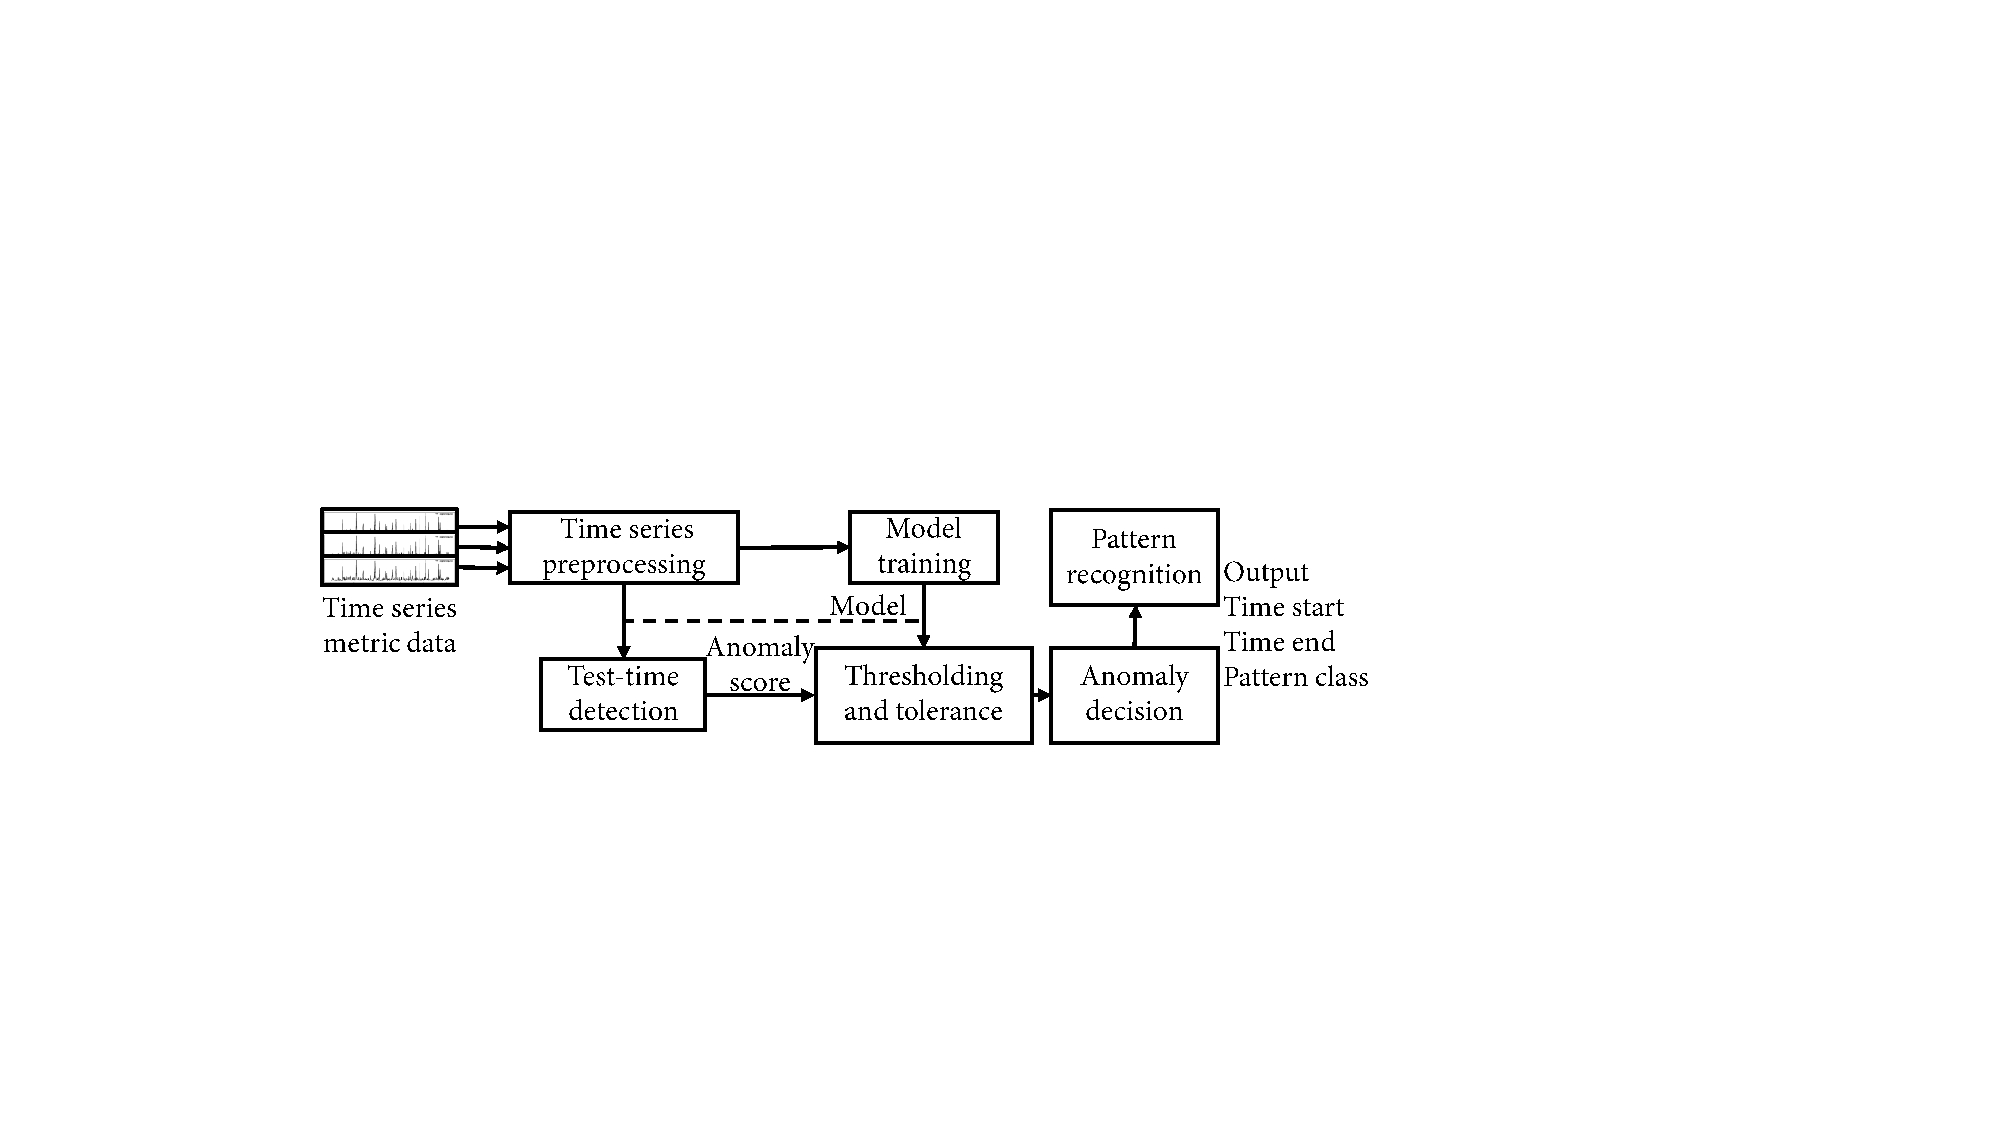
\includegraphics[width=1.0\textwidth]{gfx/chap4/metanooverview.pdf}}
\caption{Overview of Metano.}
\label{fig:metanooverview}
\end{figure}

\section{\textit{Metano}: anomaly detection and classification in metrics}\label{stability}
To formally define Metano, we consider historical observations of a part of a discrete time series representing metric data $\mathbf{x_t} = x_{t-w}, x_{t-w+1}, \dots, x_t$, where $w$ is the size of a defined sliding window over the time series and $x_{t-w}, x_{t-w+1}, \dots, x_t$ are observed values. $\phi(\mathbf{x_t}, \theta): \mathbb{R}^w \rightarrow \mathbb{R}^h \rightarrow [0, a], a \in \mathbb{R}$ is a function represented by a neural network, which maps the input time series window $\mathbf{x_t}$ to a latent representation in $\mathbb{R}^h$, and then to an anomaly score. The method learns the parameters $\theta$, and then, for each incoming instance in the prediction phase $\mathbf{x_1^{test}}, \mathbf{x_2^{test}},\dots, \mathbf{x_i^{test}}, \dots$, predicts whether it is anomalous or normal based on the anomaly scores and threshold $\tau$. If an anomaly is detected, the method classifies it into a finite set of predefined patterns $y_p \in {0, \dots, k}$ with a classifier network $\phi(\mathbf{x_i^{test}}, \hat{\theta})$.

The overall structure of Metano is shown in Figure~\ref{fig:metanooverview}, which consists of two parts, offline training and online (test-time) detection. The time series from the metric data is preprocessed. After the preprocessing, the transformed data are sent to the model training module to learn a model that captures the normal patterns of the time series and outputs an anomaly score for each observation. These anomaly scores are used by the adaptive thresholding and tolerance modules to choose threshold parameters. This offline training procedure can be carried out routinely, e.g., once per day, week, or month. 

The test-time detection module uses the trained model. An observation, $\mathbf{x_{test}}$ at time $t$, after the preprocessing, is predicted by the model to obtain an anomaly score. If the anomaly score passes the checks in the threshold and tolerance module, it will be declared as anomalous; otherwise, it is normal. Parts of the time series that are detected as anomalies are forwarded in the pattern recognition module, where a description of the anomaly will be added. Finally, Metano outputs a dictionary object containing the start timestamp of the window, end timestamp of the window, prediction, and pattern class if the prediction suggests an anomaly. 

\subsection{Time series preprocessing}\label{timeseriespreprocessing}

This step involves two parts, preprocessing in model training and test-time prediction. 
The module starts by querying the $N$ data points of a time series and forwards them into a three-stage pipeline consisting of data cleaning, normalization, and noise reduction. Figure~\ref{fig:preprocessingtimeseries} shows an overview of the preprocessing module.

\begin{figure}[htbp]
\centerline{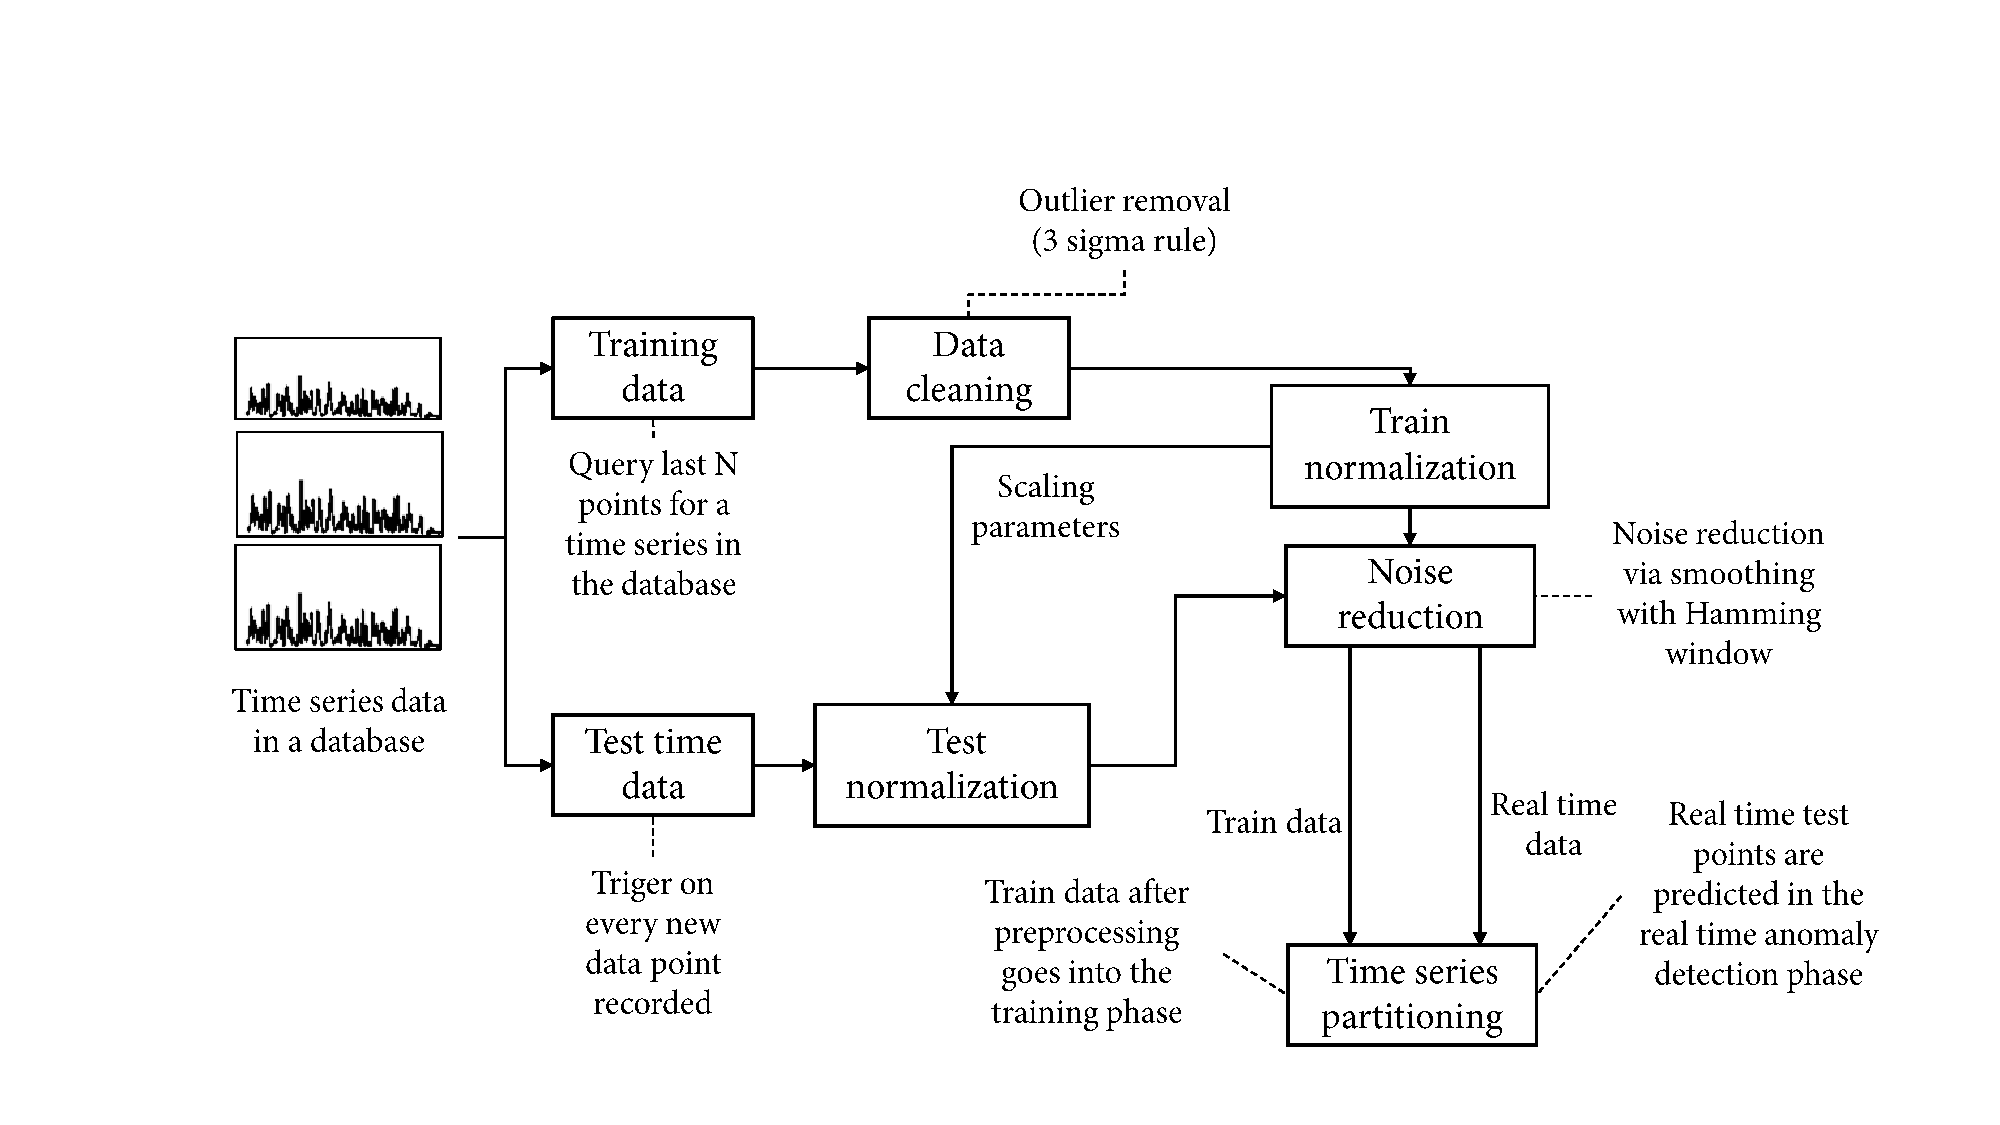
\includegraphics[width=1.0\textwidth]{gfx/chap4/timeseriespreprocessing.pdf}}
\caption{Detailed overview of the time series preprocessing part.}
\label{fig:preprocessingtimeseries}
\end{figure}

In the offline training phase, we perform data cleaning as the first step. Samples having values larger than three standard deviations from the mean are removed from the training batch, according to the three-sigma rule~\cite{pukelsheim1994three}. This is important for robustness and to remove possible anomalies in the training data, as labels are not available. The values are then normalized using min-max scaling (0, 1). Normalization is required and makes the optimization function of the neural network well-conditioned, which is crucial for convergence~\cite{ioffe2015batch}. The min-max normalization is expressed by

\begin{equation}\label{eq8}
\mathbf{x_{t, scaled}} = \frac{\mathbf{x}_t - min(\mathbf{X})}{max(\mathbf{X}) - min(\mathbf{X})},   
\end{equation}

where $min(X)$ and $max(X)$ are saved as scaling parameters and are later used for normalization in the test data. Lastly, in the pipeline, we apply smoothing for noise removal and robustness against small deviations. To this end, the time series is convolved with a Hamming smoothing filter defined with its optimal parameters~\cite{1163506} and size of $M$ as

\begin{equation}\label{eq9}
f(n)=0.54-0.46 \cdot cos\bigg( \frac{2\pi n}{M-1}\bigg), 0 \leq n \leq M-1.
\end{equation}

During the test-time prediction, the time series follows the same preprocessing steps. In the normalization module, $min(X)$ and $max(X)$ are the previously obtained values during the model training part. 
This implies that time series values, which have values larger (smaller) than $max(X)$ ($min(X)$) obtained during the training, will have normalized values larger than 1.0 (smaller than 0.0). 

% \begin{figure}[htbp]
% \centerline{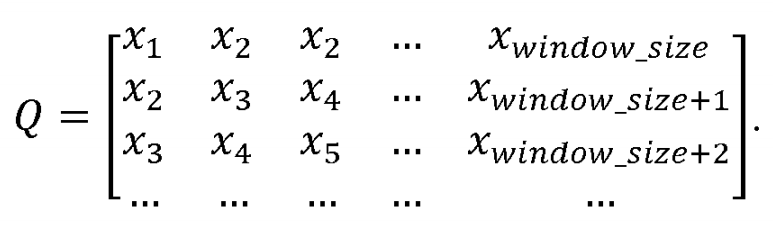
\includegraphics[scale=0.6]{gfx/chap4/splittingtimeseries.png}}
% \caption{Partitioning of a time series with stride=1.}
% \label{fig:timeseriespartitioning}
% \end{figure}

\subsubsection*{Time series partitioning}\label{reshapingtimeseries}
The next step in the pipeline is to transform the time series data into windowed format. In contrast to methods that perform anomaly detection on finite time series data (already windowed, e.g., ECG signals~\cite{acker2017patient}), here we formulate the anomaly detection on sliding windows of the time series, which enables test-time prediction in streaming fashion. Therefore, we define $w$, which is the size of the sliding window. The window is applied to the time series and leads to a training data shape of $(N-w, w, 1)$,

\begin{equation}\label{timeseriespartitioning}
X_{train} = 
\begin{pmatrix}
x_1 & x_2 & \dots & x_{w}\\
x_2 & x_3 & \dots & x_{w+1} \\
\dots \\
x_{N-w} & x_{N-w+1} & \dots & x_{N} \\
\end{pmatrix}_{(N-w) \times w.}
\end{equation}

In the test-time prediction, for each new collected value of the time series, a window of points $x_{test}$ with a size of $w$ is formed, preprocessed, and fed to the network for prediction.

\subsection{Network architecture}
To learn the patterns of the time series data representing the normal system behavior, we design an architecture based on a VAE~\cite{kingma2013auto}, which maps observations (i.e.,input values) to stochastic (i.e., latent) variables, and then reconstructs the input (Figure ~\ref{fig:vae}. The dimensionality of the latent variables is lower than the dimensionality of the input. Therefore, the latent variables are enforced to capture salient features of the normal patterns of the time series.
% These latent variables in VAE are parameters of a known probability distribution (e.g., Gaussian). VAE is a generative model, which learns approximations of the data distributions. 
To detect anomalies, the model uses a window of a time series as an input and performs reconstruction. The reconstruction for normal time series data, similar to those used for model training, is expected to provide a small reconstruction error, as the model is trained by optimizing the error loss function. The reconstruction error for an anomaly sample is expected to be large, as the model is not trained to reconstruct such time series data~\cite{an2015variational}. The decision for anomaly is then based on a threshold on the reconstruction error.

The optimization of VAE relies on variational inference. The variational inference method approximates intractable probability densities through optimization. We consider a probabilistic model with observations $\mathbf{X}=x_{1:n}$, continuous latent variables $\mathbf{z}=z_{1:m}$, and model parameters $\theta$. The task is to compute the posterior distribution

\begin{equation}\label{posterior}
    p(\mathbf{z} \vert \mathbf{X},\theta)=\frac{p(\mathbf{z},\mathbf{X} \vert \theta)}{\int_z p(\mathbf{z},\mathbf{X} \vert \theta)}.
\end{equation}

The computation requires marginalization over the latent variables $\mathbf{z}$, which is intractable. In variational methods, a distribution family is chosen over the latent variables with its variational parameters $q(z_{1:m} \vert \nu)$. The parameters that lead to $q$ as close as possible to the posterior of interest are estimated through optimization~\cite{jordan1999introduction}. However, the true posterior often is not in the search space of the distribution family and thus the variational inference provides only an approximation. 


\begin{figure}[!t]
\centerline{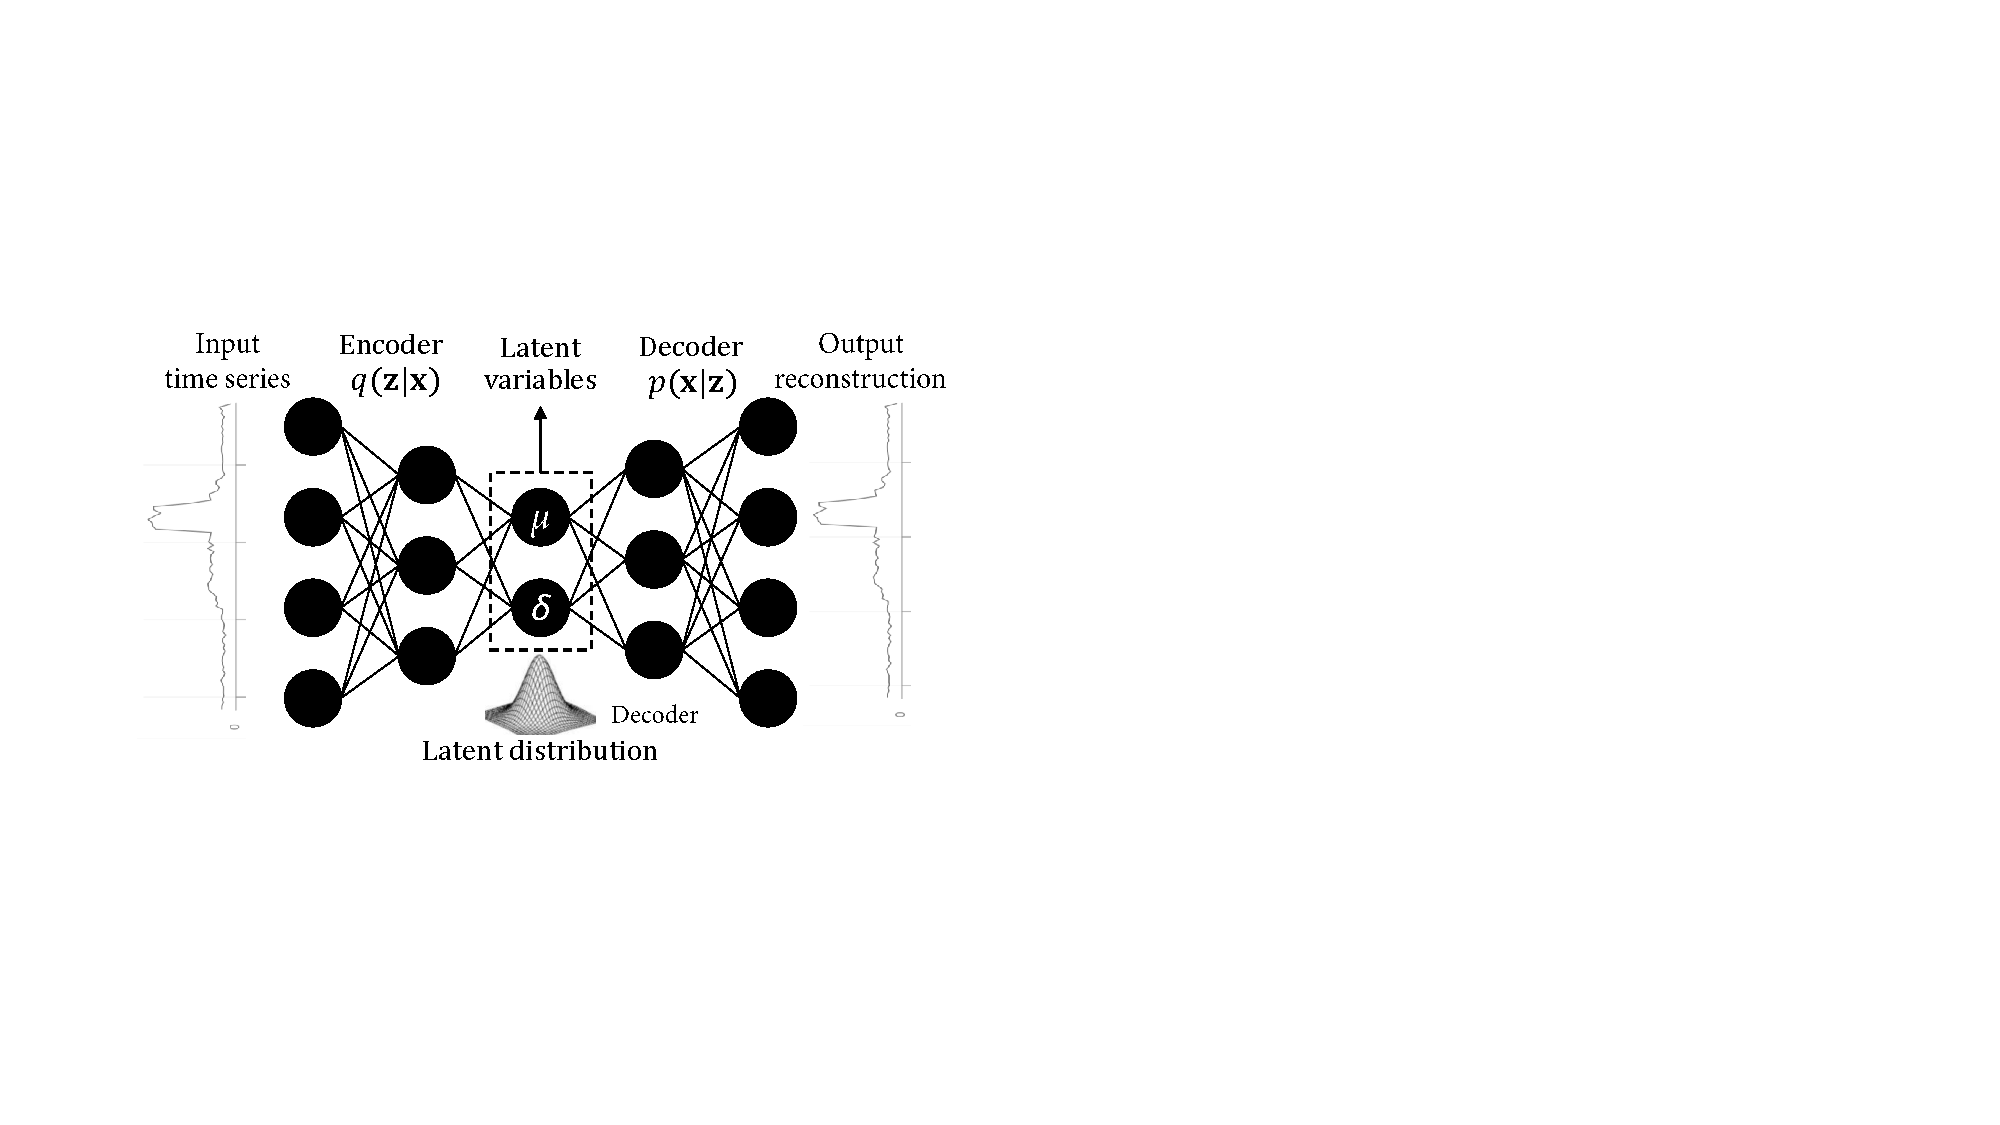
\includegraphics[width=0.7\textwidth]{gfx/chap4/vae.pdf}}
\caption{Architecture of a VAE.}
\label{fig:vae}
\end{figure}


The similarity between the two distributions is measured by the Kullback–Leibler (KL) divergence, a measure of the difference of one probability distribution from a reference probability distribution,

\begin{equation}\label{kl}
    \mathrm{KL}(q \Vert p) = \mathbb{E}_q\left[\log \frac{q(\mathbf{z})}{p(\mathbf{z} \vert \mathbf{x})}\right].
\end{equation}

Direct and exact minimization of the KL divergence is not possible. Instead, as proposed in \cite{jordan1999introduction}, a lower bound on the log-marginal likelihood is constructed,

\begin{align}
    \log p_\theta(\mathbf{x}) \geq \log p_\theta(\mathbf{x}) &- \mathrm{KL}(q(\mathbf{z}\vert \mathbf{x})\Vert p_\theta(\mathbf{z}\vert \mathbf{x})) \label{elbo1} \\ 
    = \mathbb{E}_{q(\mathbf{z} \vert \mathbf{x})}\left[\lambda \log p_\theta(\mathbf{x}|\mathbf{z})\right]
    &- \beta \mathrm{KL}\left[q(\mathbf{z}|\mathbf{x}), p(\mathbf{z})\right] \label{elbo2} \\
    &= \mathrm{ELBO(\mathbf{x})} \nonumber,
\end{align}

where $\lambda$ and $\beta$ are weights in the Evidence Lower Bound (ELBO). In practice, $\lambda=1$ and $\beta$ is slowly annealed to 1 to form a valid lower bound on the evidence~\cite{bowman2015generating}. In VAEs, the ELBO function is optimized by gradient descent using the reparametrization trick, while the parameters of the distributions $p$ and $q$ are obtained by neural networks (encoder and decoder). In Equation~\ref{elbo2}, the first term represents the reconstruction error, while the second corresponds to the regularization. The VAE can only learn the distribution from the windows of the metric time series data. However, it is still not able to recognize temporal dependencies (sequence) in the data.

% The VAE, as described, and shown in Figure~\ref{fig:vae}, is utilized successfully for anomaly detection in metric data from software systems~\cite{donut}. However, owing to the complex temporal dependence of the time series, the anomaly detection is still remains to be a challenging task.

The second property of the time series data that needs to be addressed in the model design is the sequential dependence between values. To preserve the sequential nature of the metric data, in the encoder and decoder parts of the VAE, RNNs are utilized~\cite{rumelhart1986learning}. They are a deterministic type of neural network where the connections between neurons form a directed cycle. This deterministic part of the autoencoder is crucial to capture long-term complex temporal information between the values in the time series observation.


\begin{figure}[!t]
\centerline{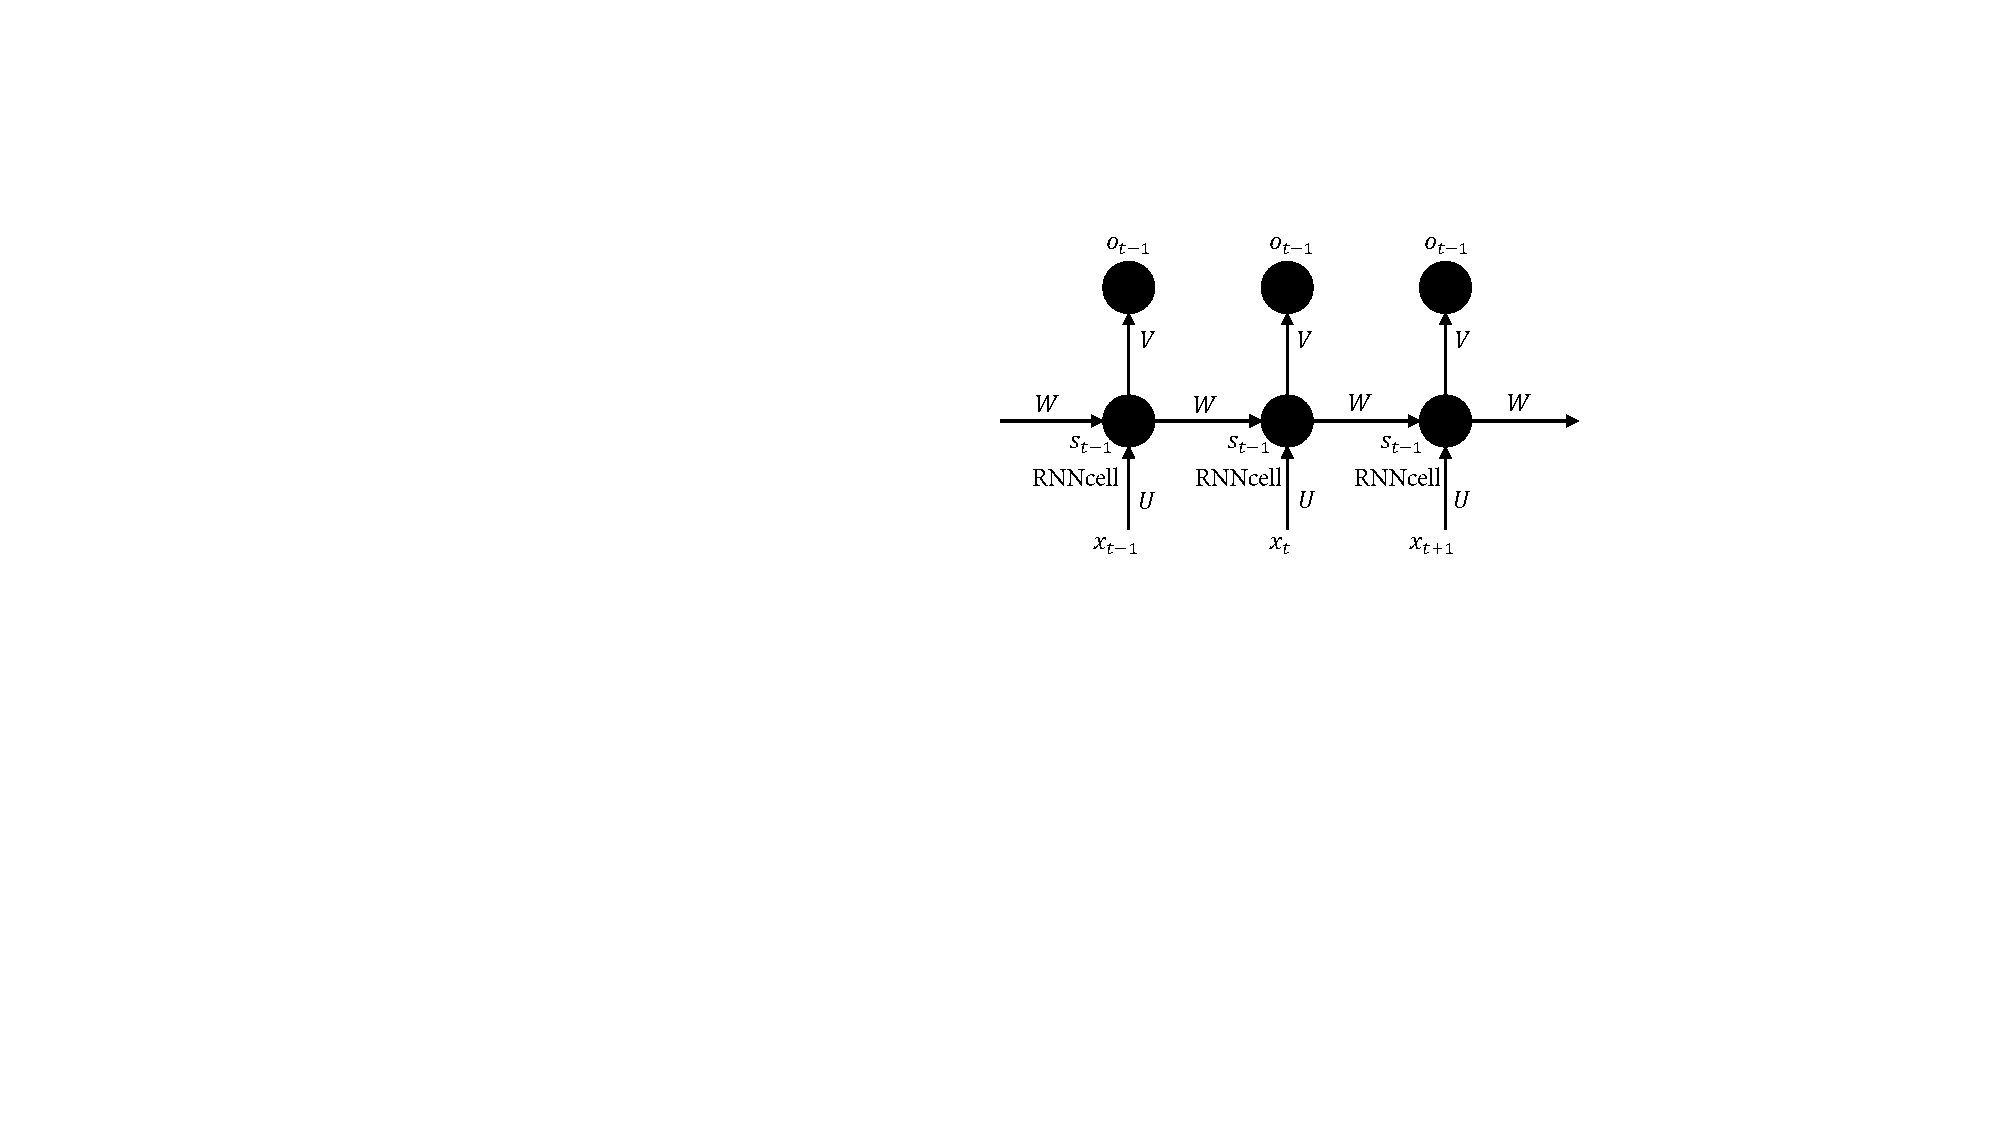
\includegraphics[scale=1.1]{gfx/chap4/rnn.pdf}}
\caption{Architecture of the RNN.}
\label{figrnn}
\end{figure}

In a vanilla RNN, as presented in Figure~\ref{figrnn}, the largest issue is the vanishing gradient problem~\cite{hochreiter1998vanishing}. Numerous solutions exist for this problem, which well perform in practice. The most used RNN types are LSTM~\cite{hochreiter1997long} and GRU~\cite{cho2014properties} cells, which are used in Metano. The GRU cell is a simpler version of the LSTM, which requires less computational resources. The GRU computes an update gate based on the current input vector and hidden state,

\begin{equation}\label{eq4}
  z_t = \sigma(W^{(z)}x_t + U^{(z)}s_{t-1}),
\end{equation}

and then computes the reset game similarly but with different weights,

\begin{equation}\label{eq5}
    r_t=\sigma(W^{(r)}x_t + U^{(r)}s_{t-1}).
\end{equation}

The new memory content is

\begin{equation}\label{eq6}
    \tilde{s_t}=\tanh(Wx_t + r_t \circ U s_{t-1}).
\end{equation}

If the reset gate is 0, this ignores the previous memory and stores only the new information.
The final memory content combines the current and previous timesteps, 

\begin{equation}\label{eq7}
    s_t = z_t \circ s_{t-1} + (1-z_t)\circ \tilde{s_t}.
\end{equation}

The update gate $z$ controls the effect of the past state on the state at timestamp $t$.
If $z$ is close to 1, it can copy information in that unit through numerous time steps. Units with short-term dependencies often have active reset gates. 

This gated flow of the information enables the GRU to model long-term dependencies~\cite{chung2015recurrent}.

We replace the encoder and decoder, i.e., $q(\mathbf{z}|\mathbf{x})$ and $p(\mathbf{x}|\mathbf{z})$, with GRUs (Figure~\ref{fig:vae}. In this regard, we address the stochasticity and temporal dependence in the model design. The overall architecture of the model is shown in Figure~\ref{figmodeltraining} and described below. The objective for model training with gradient descent is Equation~\ref{elbo2}.

\textbf{The input layer} has $w$ units; each of them contains the metric value.

\textbf{The first hidden GRU layer} contains $w/2$ GRU cells for each timestep in the input window. $w/2$ as a hidden dimension size is chosen to restrict and contract the architecture, thus enforcing the hidden states to learn salient features of the time series~\cite{Goodfellow-et-al-2016}. Each of the $w$ input units is fed to the corresponding GRU block. In the first timestep $t=0$, the $0^{th}$ value of the time series is fed. 
The abstract representation learned in the 16 GRU cells, according to Equation~\ref{eq4}-\ref{eq7}, is then propagated to the next timestep $T=1$, where the $1^{st}$ value of the time series of the window is fed, and so on.
We can condition the reconstruction of the next point considering the input of past points. In this regard, in the last timestep, we have an abstract representation of the window of points, which has a salient information for that part of the time series.

\begin{figure}[!t]
\centerline{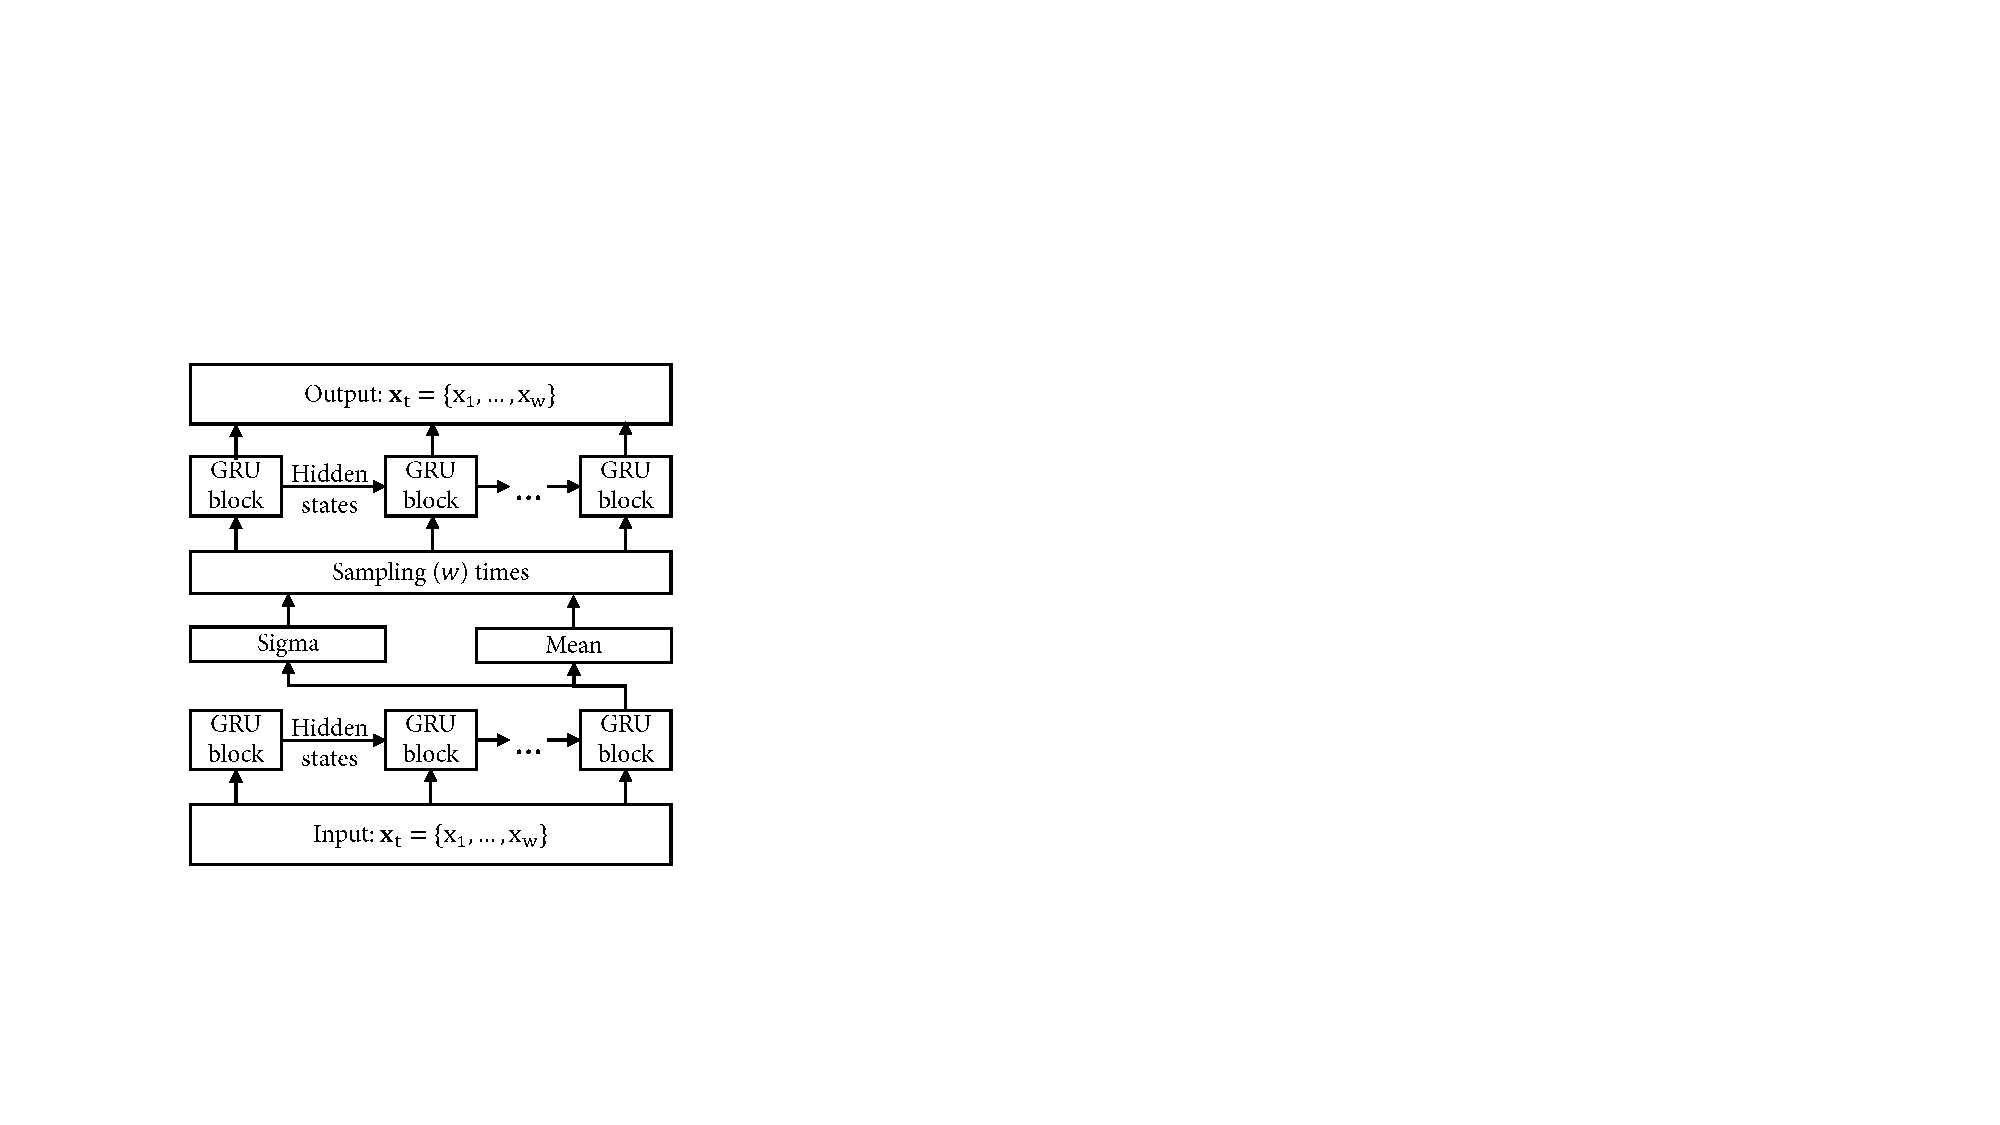
\includegraphics[width=0.5\textwidth]{gfx/chap4/modeltraining.pdf}}
\caption{Model architecture.}
\label{figmodeltraining}
\end{figure}

\textbf{The sampling layer} represents the key part to be able to learn the stochastic process of the time series. This layer is the core part of the VAE and consists of $w/4$ units for the mean and variance of the Gaussian distribution. Gaussian distribution has many beneficial properties, such as analytical evaluation of the KL divergence in the variational loss, and also we can use the reparametrization trick for efficient gradient computation~\cite{kingma2013auto}. It does not matter so much what distribution latent variables follow since using a non-linear decoder can mimic arbitrarily complicated distribution of observations. However, one of the apparent advantages of using the Gaussian in the sampling layer is that it allows easy generation of new samples by sampling in the latent space. 

The model learns the data distributions as an approximation to the multivariate Gaussian. The sampling layer only performs sampling from a multi-variate Gaussian distribution with the learned mean and variance. The complexity of the model allows to learn multiple distributions activated depending on the input.

\textbf{The repeat layer} repeats the sampling layer $w$ times, which needs to be fed into the last hidden GRU layer and utilized for the decoder and reconstruction of the input. This layer is acts like a copy function used for implementation purposes only.

\textbf{Output/GRU layer:} The network uses the output from the previous layer as the input, learns an abstract representation, and, as an output, has the same number $w$ of timesteps, as the output $\mathbf{\hat{x}}$ in autoencoder architectures is the same as the input $\mathbf{x}$. This layer reconstructs the time series.

Through the training of this neural architecture with the loss function of the VAE in Equation~\ref{elbo2} on normal time series data, normal patterns from the data are learned. Once the model of the normality in the system is trained, it can be utilized for anomaly detection by performing reconstructions of the test-time time series.

\subsection{Dynamic error threshold}\label{ch:metrics:sec:metano:subsec:threshold}
The difference between a prediction and observed value of the time series vector is measured by the mean squared error (MSE),

\begin{equation}\label{eqMSE}
MSE=\frac{1}{w}\sum(\mathbf{x_t}-\mathbf{\hat{x_t}})^2.
\end{equation}

Instead of setting a fixed error threshold for anomaly detection, we utilize a validation set (part of the training data) for threshold selection. This is beneficial for the operators and users of Metano, as they do not have to tune and calibrate the threshold in each model training and for every metric. For each window of time series points in the validation set, we apply the model produced by the training set and calculate the MSE between the prediction (reconstruction) and actual sample. At every time step, the errors between the predicted vectors and actual vectors in the validation group are modeled by a Gaussian distribution. We choose the Gaussian distribution to model the MSEs, as per the central limit theorem~\cite{rosenblatt1956central} such samples follow normal distribution.
In the test-time prediction, if the error between reconstructed and observed windows of events (MSE) is within a high level of confidence interval of the above Gaussian distribution, it is considered normal; otherwise, it is considered anomalous.

\subsection{Test-time prediction}
\label{realtimedetectionunstablebehavior}
This module receives data from the preprocessing module described above. The latest model along with the saved training parameters are loaded and used for prediction. For each new value of the time series, the past values forming a window $\mathbf{x_t} = \{x_{t-w}, x_{t-w+1}, ..., x_t\}$ are fed as an input for prediction. The reconstruction error $MSE_{test}$ and probability under the Gaussian distribution of the threshold, obtained during the validation procedure, are computed,

\begin{equation}\label{eqP}
P_{test} = 1 - P(X > MSE_{test}).
\end{equation}


\subsubsection{Tolerance: FP reduction}\label{tolerance}
In large-scale system architectures, a single anomalous point often exists in the time series. However, this does not imply that something is wrong in the particular component. For example, it can be attributed to a small bottleneck in the disk usage or in one of the many components or services. The detection of anomalies having larger impacts enables the DevOps to focus on the most critical potential failures.

We define the tolerance and probability error threshold as parameters. The tolerance represents the allowed number of anomalous windows that have $P_{test}$ larger than the threshold before it flags the whole period as anomalous. In practical scenarios, the tolerance parameter usually is in the range of 1 to 100, but is dependent on the dynamics of the system. The probability outputs $P_{test}$ are kept in a queue with the same size (tolerance) for each new window.  
Each time a new sample is shown to the network to be reconstructed, assigned with the probability of being anomalous, and added to the queue, the tolerance module checks whether the average probability of the samples in the queue

\begin{equation}\label{eqtol}
P_m=\frac{1}{tolerance}\sum_{i}^{tolerance} P_{test(i)},
\end{equation}

is larger than the error threshold. If this is the case, the submodule flags this part of the time series as unstable and reports an anomaly. 
In this regard, we can address the problem of having too many FPs and allow the user to set the sensitivity of the algorithm on his/her demand.
The output of the module is a tuple (first anomaly window timestamp, last anomaly window timestamp).

\subsection{Faulty pattern classification}

Identifying an anomaly without providing insights into its nature is of limited importance. The user may be interested in detecting particular types of anomalies reflected in the time series (incremental, mean shift, gradual increase, cylinder, etc.).  Therefore, we provide a module based on a one-dimensional CNN~\cite{lecun1995convolutional}, which, with a window of the time series as an input, can classify into one of the user-defined patterns described above. The architecture of the CNN consists of a combination of convolutional and max-pooling layers followed by a soft-max layer, which distributes the probability for given pattern. A similar study on time series classification has been recently reported \cite{zhao2017convolutional}.

\begin{figure}[htbp]
\centerline{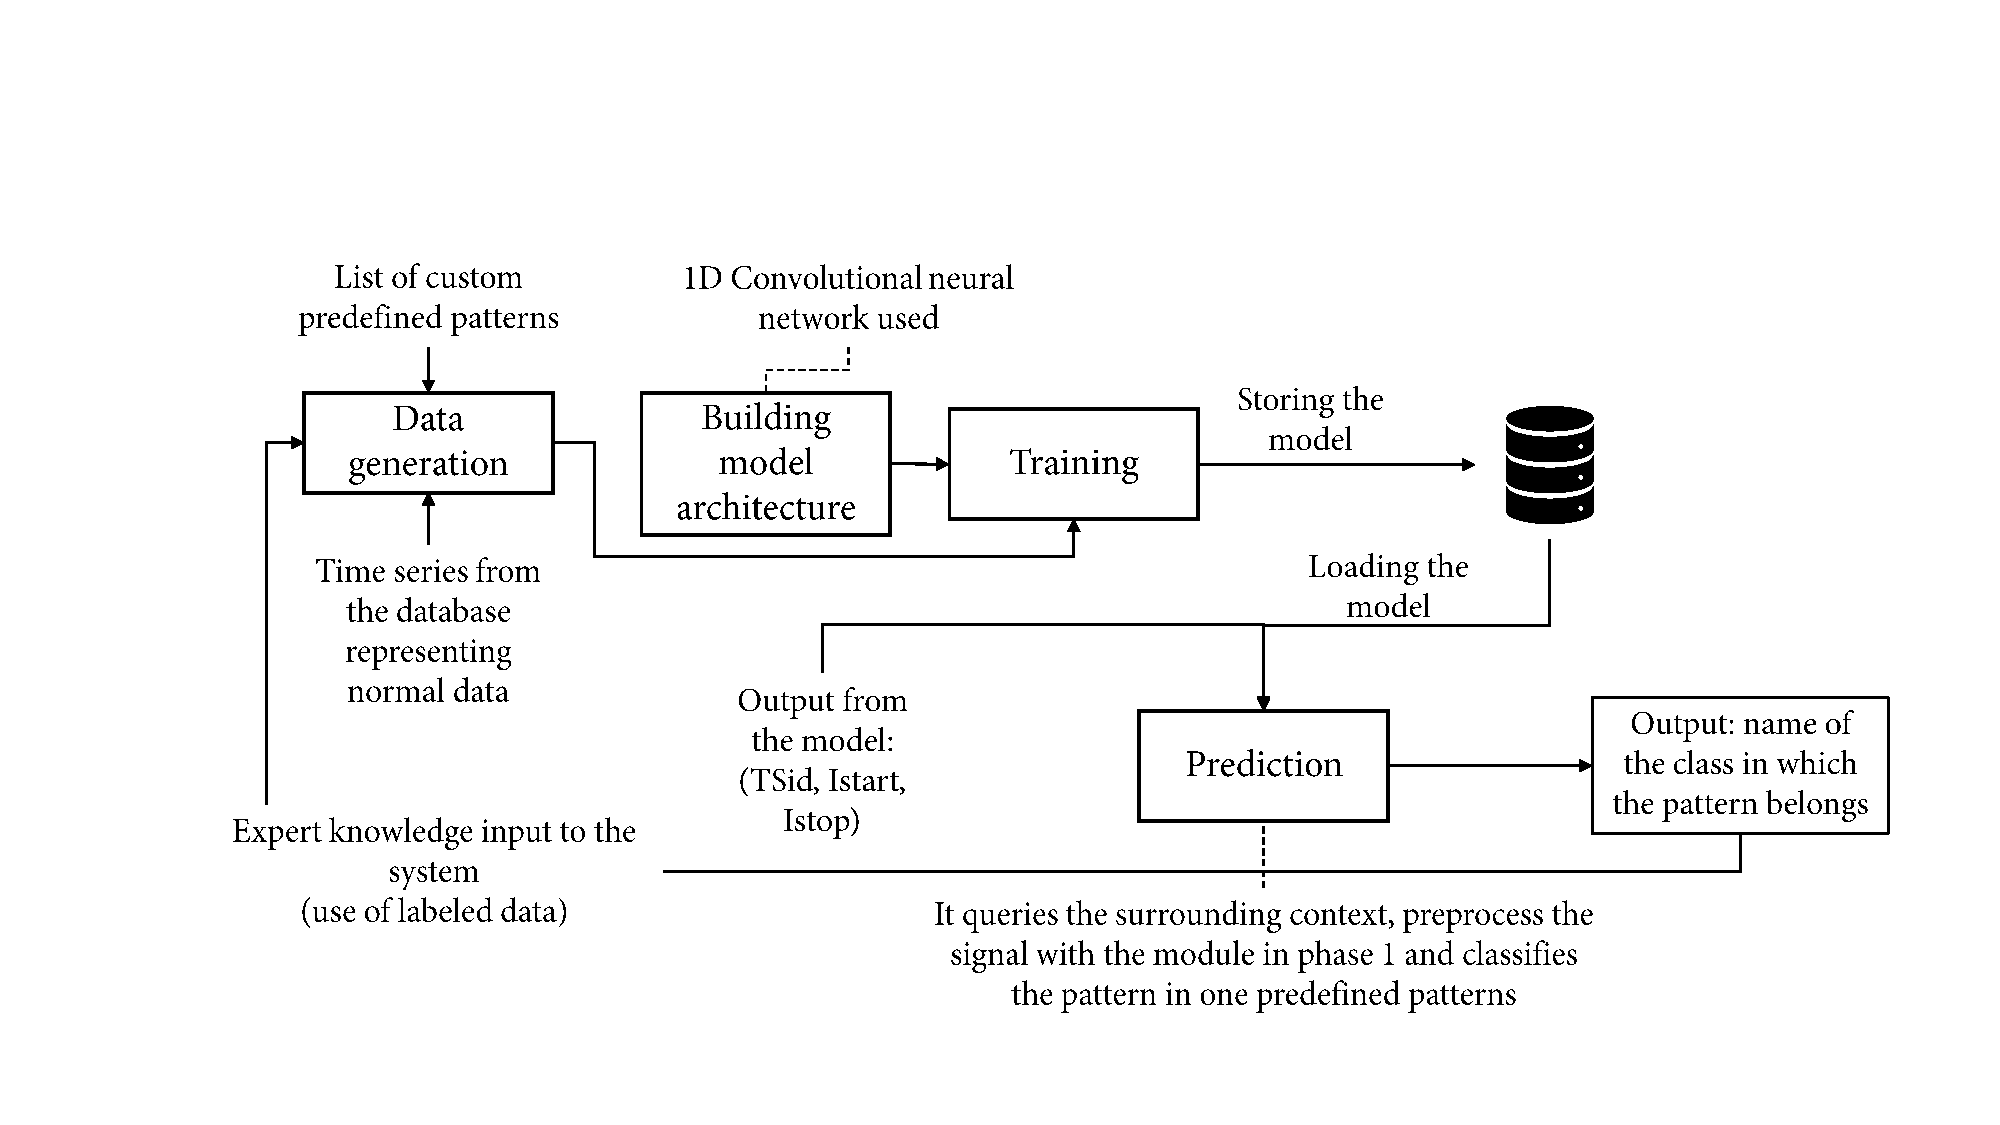
\includegraphics[width=1.0\textwidth]{gfx/chap4/patternclassification.pdf}}
\caption{Anomaly pattern classification.}
\label{fig:patternclassification}
\end{figure}

We show a detailed overview of this module in Figure~\ref{fig:patternclassification}. The data utilized to train the previously described model (see Eq.~\ref{timeseriespartitioning}) are queried and utilized to represent the normal class. The preprocessed normal data are concatenated with the user-defined patterns. These are then fed as an input to the CNN model. 

The model architecture consists of three (convolutional, max-pooling) layers with dropout regularization. The last layer, typical for multi-class classification, is fully connected with the softmax function for computing the probability distribution over the classes. The convolutional networks are naturally invariant to translation, which makes them suitable for faulty pattern detection with a sliding window over the time series. The network is trained using the described data and the model is saved and used for prediction. 

The classifier triggers when the test-time prediction detects an anomaly. The classifier module receives the output from the test-time prediction and requests the particular time series within the provided anomalous time interval. Using the trained model, it maps each sliding window to the predicted class. If the particular pattern is recognized, the module will output the name of the class to which the pattern belongs and will flag the interval as anomalous.

\section{Evaluation}\label{metrics:evaluation}
In this section, we describe three experimental datasets. We then carry out experiments to show the effectiveness and performance of our model. The methods in this chapter are implemented as prototypes in Python using Keras~\cite{chollet2015keras}. The evaluation on the collected datasets was carried out on a regular personal computer with the following specifications: GPU-NVIDIA GTX 1060 6GB, 1TB HDD, 256 SSD, and Intel(R) Core(TM) i7-7700HQ CPU at 2.80 GHz. 
We performed series of experiments to learn the sequence with LSTMs and other deterministic models. The models learned the running mean of the time series. Therefore, we discard comparisons to these methods in this section. In the experiments, Metano is compared to Donut~\cite{donut}, a state-of-the-art univariate metric time series anomaly detection approach based on VAE. 

\subsection{Microservice architecture testbeds}
\begin{figure}[!t]
\centerline{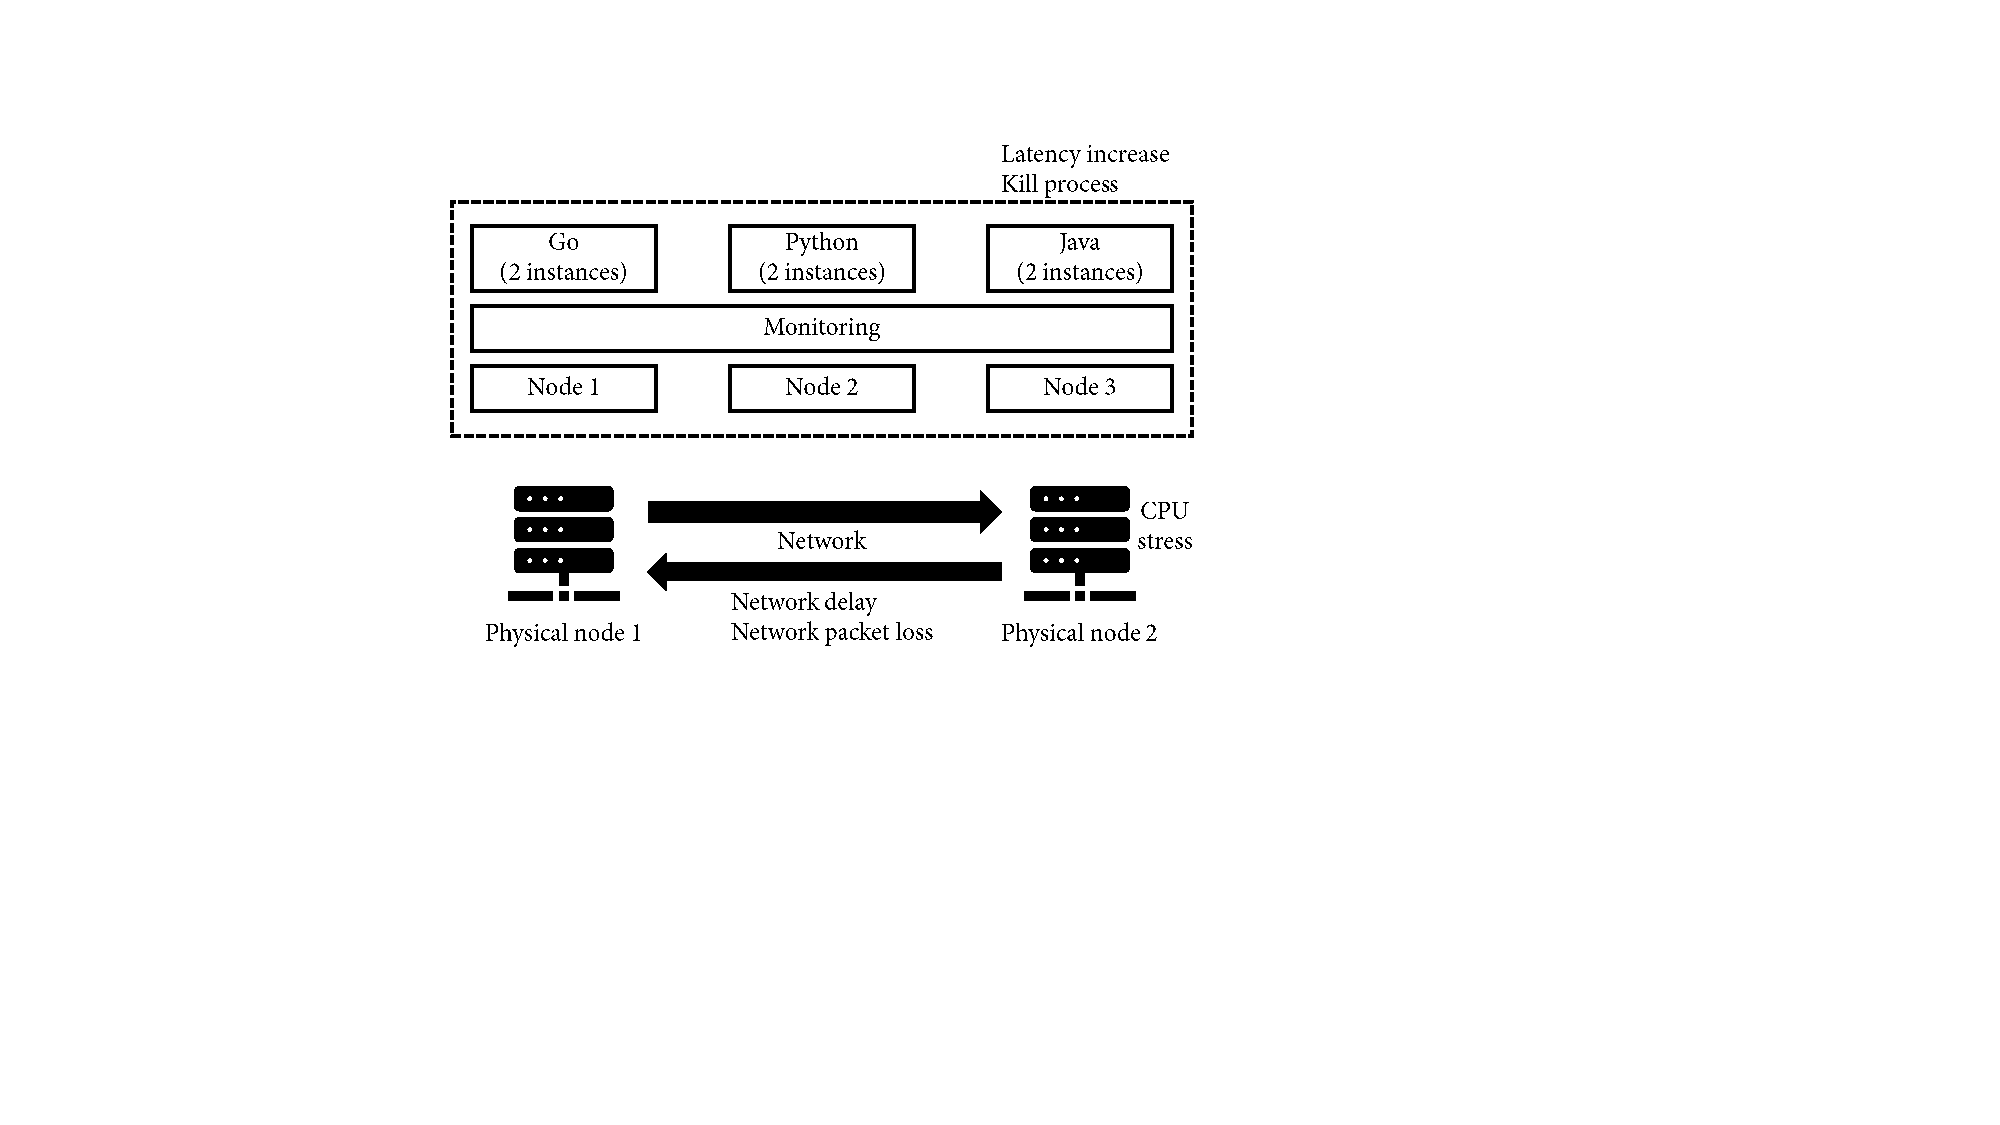
\includegraphics[width=0.8\textwidth]{gfx/chap4/artificialmicroservicetestbed.pdf}}
\caption{Experimental microservice system architecture.}
\label{testbed}
\end{figure}
\textbf{Artificial microservice response times.}
We created an experimental microservice system to evaluate Metano on  representative anomaly scenarios for microservice architectures. For the setup, we used two physical nodes and three virtual machines with enabled tracing, with running instances of Python, Go, and Java applications, respectively. The testbed architecture is shown in Figure~\ref{testbed}. The collected data include the response time metric for each endpoint in the microservice architecture.

To simulate the anomalies, we injected timed physical network anomalies in the form of delay and packet loss, physical node anomalies in the form of CPU stress, and service anomalies in the form of response time increase. They led to six different scenarios on different endpoints in the system, described below. 

\begin{itemize}
    \item Scenario 1: Baseline without anomaly - represents the normal operation (no anomalies) of the system and is used to train the detection algorithms.
    \item Scenario 2: Service latency increase - profile 1 (injection of latency (1 s) for a duration of 15 s).
    \item Scenario 3: Service latency increase - profile 2 (injection of latency (1, 5, 30 s) for a duration of 30 s, 1 min, and 10 min on nodes 1,2,3).
    \item Scenario 4: Network packet loss - A packet loss (10\%, 20\%, 30\%) is injected on one of the network links for durations of 1, 5, and 10 min. 
    \item Scenario 5: Network delay - A network delay (1, 2, 3 s) is injected on the network for durations of 1, 5, and 10 min.
    \item Scenario 6: Server process dies -  One process is killed on nodes 1 and 3 for durations of 1, 5, and 10 min.
\end{itemize}


\textbf{Response times from production-cloud data.}
Even in small controlled experimental setups, the noise is high and the time series changes rapidly over time. This already poses challenges for the anomaly detection algorithm. However, testing the approach on large-scale production cloud data is required to show the viability of the approach.

The dataset contains response times of three main services for a period of four days, obtained from a large-scale production cloud. 
The signal-to-noise ratio in the data is small as numerous components affect the response time of microservices. The time series evolves faster and changes its distribution over time while having a stochastic behavior. The time series of the response time from one of the production services was already plotted and discussed in~\autoref{ch:concepts:sec:anomalydetectionindistributedsoftwaresystems:subsec:metric}.

\textbf{Sockshop microservice testbed.} In addition to the artificially created microservice architecture testbed, we set a second testbed on Google Cloud Engine\footnote{https://cloud.google.com/compute} where we run the Sock-shop\footnote{https://microservices-demo.github.io/} microservice benchmark consisting of seven microservices. The monitoring tools include node-exporter\footnote{https://github.com/prometheus/node\_exporter}, Cadvisor\footnote{https://github.com/google/cadvisor}, and Prometheus\footnote{https://prometheus.io}. Sock Shop simulates the user-facing part of an e-commerce website, which sells socks. It is intended to aid the demonstration and testing of microservice and cloud native technologies. We also developed a workload generator to send requests to different services. To inject the performance issues in microservices, we customize the Docker images of the services by installing the fault injection tools. Three types of faults were injected into the Sock shop services, (1) network anomalies by increasing the latency, (2) CPU hog, and (3) memory leak, by exhausting the CPU and memory resources in the container with stress-ng. For each anomaly, we repeated the experiments multiple times in the duration of at least 2 min. To train the model, we collect data for 1 h in the normal status. The data include a total of seven metrics for each service (CPU, memory, and network usage, on host and container levels, and service response time).


% Out of them, we selected three services of interest. 
% The anonymized names along with the count of the samples is given in Table \ref{tableclusters}

% \begin{table}[!t]
% \centering
% \caption{Ser for analysis.}
% \begin{tabular}{ll}\hline
% ClusterID		&Count\\ \hline
% \{host\}/v1/\{p\_id\}/cs/limits		&12900\\
% \{host\}/v1/\{t\_id\}/cs/delete		&2732\\
% \{host\}/v2/\{t\_id\}/servers/detail		&6468\\
% \hline 
% \end{tabular}
% \label{tableclusters}
% \end{table}


\begin{table}[htbp]
\centering
\caption{Metano: F1 scores for 15 endpoints in five anomaly scenarios of the experimental testbed data.}
\resizebox{1.0\textwidth}{!}{%
\begin{tabular}{l|cc|cc|cc|cc|cc}
\hline
\multicolumn{1}{c|}{Scenario}                                 & \multicolumn{2}{c|}{S2} & \multicolumn{2}{c|}{S3} & \multicolumn{2}{c|}{S4} & \multicolumn{2}{c|}{S5} & \multicolumn{2}{c}{S6} \\ \hline
\begin{tabular}[c]{@{}l@{}}Endpoint ID/\\ Method\end{tabular} & Donut      & Metano     & Donut      & Metano     & Donut      & Metano     & Donut      & Metano     & Donut      & Metano     \\ \hline
1                                                             & -          & -          & 0.85       & 0.85       & 0.93       & 0.95       & 0.95       & 0.98       & 0.99       & 0.99       \\
2                                                             & -          & -          & -          & -          & 0.99       & 0.99       & 0.93       & 0.98       & -          & -          \\
3                                                             & -          & -          & -          & -          & 0.98       & 0.96       & 0.98       & 0.99       & 0.97       & 0.96       \\
4                                                             & -          & -          & 0.90       & 0.99       & -          & -          & -          & -          & -          & -          \\
5                                                             & -          & -          & -          & -          & 1.0        & 1.0        & 0.95       & 0.98       & 0.97       & 0.97       \\
6                                                             & -          & -          & 0.93       & 0.98       & -          & -          & -          & -          & 0.81       & 0.86       \\
7                                                             & -          & -          & 0.96       & 0.95       & 0.96       & 0.98       & 0.92       & 0.97       & -          & -          \\
8                                                             & -          & -          & 0.98       & 0.98       & -          & -          & -          & -          & -          & -          \\
9                                                             & -          & -          & 0.88       & 0.92       & 0.92       & 0.91       & 0.99       & 0.99       & 1.0        & 1.0        \\
10                                                            & 0.85       & 0.90       & 0.87       & 0.95       & 0.93       & 0.95       & 0.92       & 0.99       & 0.94       & 0.98       \\
11                                                            & -          & -          & 0.96       & 0.96       & -          & -          & -          & -          & -          & -          \\
12                                                            & 0.89       & 0.85       & -          & -          & 0.79       & 0.83       & 1.0        & 0.99       & 0.95       & 0.97       \\
13                                                            & 0.90       & 0.95       & 0.91       & 0.98       & -          & -          & 0.91       & 0.94       & 0.96       & 0.99       \\
14                                                            & 0.91       & 0.99       & 0.87       & 0.95       & -          & -          & -          & -          & 0.94       & 0.98       \\
15                                                            & -          & -          & 0.86       & 0.97       & 0.95       & 0.95       & 0.99       & 0.98       & 1.0        & 1.0        \\ \hline
\end{tabular}\label{table_res_vae}
}
\end{table}
\subsection{Results and discussion}




\noindent\textbf{Artificial microservices response times.}
The F1 scores of Metano and Donut are shown in Table~\ref{table_res_vae} for all 15 endpoints in our experimental testbed across the five different scenarios. The number of injected anomalies depends on each scenario and endpoint. The missing values in Table~\ref{table_res_vae} imply that the anomaly did not affect those endpoints. 

Notably, the described approach in this chapter is comparable to or outperforms Donut~\cite{donut}. Overall, the results in the table and figure indicate that the combination of generative models, such as the VAE with GRU units, that extract temporal information is effective. The method generalizes over different anomaly scenarios. The highest scores are observed in S5 and S6, where the anomalies are most reflected in the values.

In Figure~\ref{scenarios}, scenarios 5 and 6 are illustrated, where the method successfully flags the majority of anomalous values. The method successfully flags almost all anomalous events. False positives are observed only around the 800-th and 1250-th data points of the time series, where the response time is increased owing to the considerable noise. 

Overall, the method performs comparably well, successfully handling variety of anomalies.
\begin{figure*}[!t]
     \centering
     \subfloat[][]{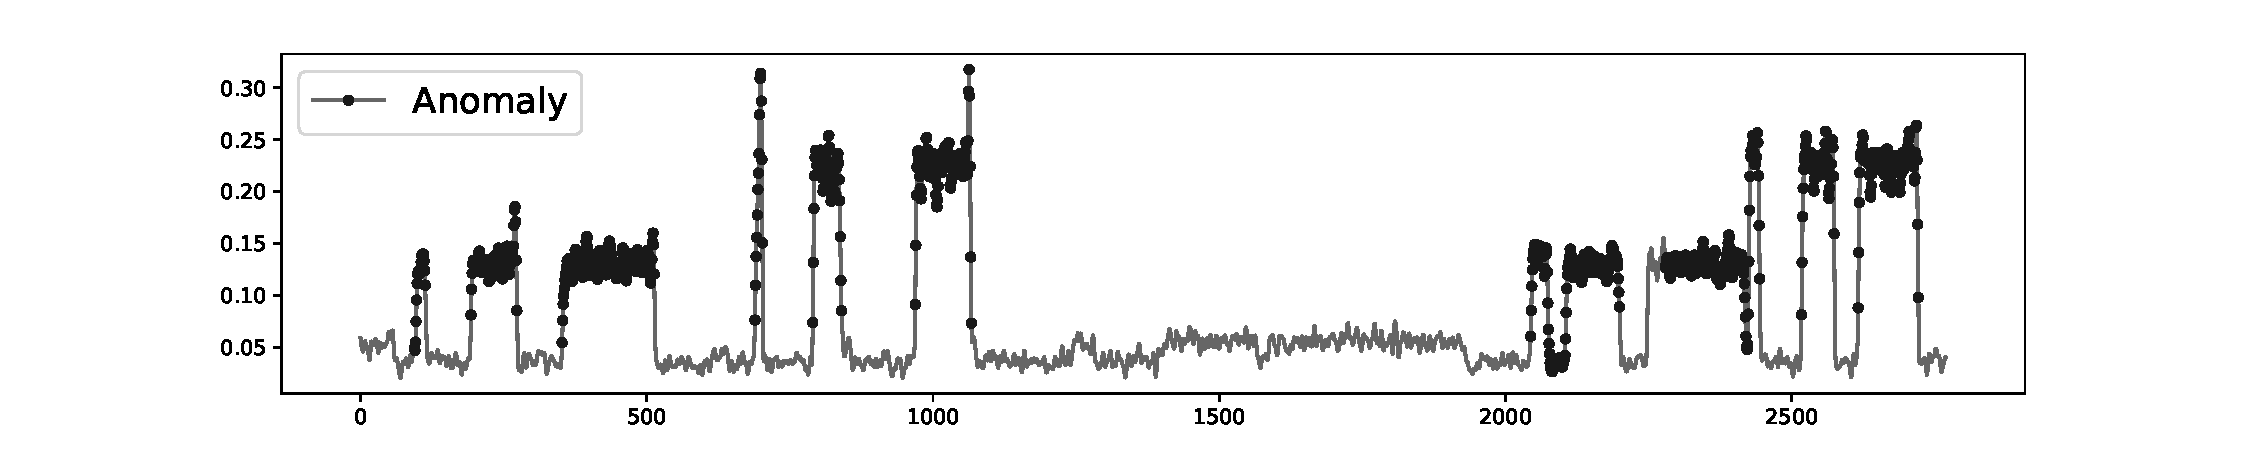
\includegraphics[width=0.48\textwidth]{gfx/chap4/scenario5.pdf}\label{scenario6}}
     \subfloat[][]{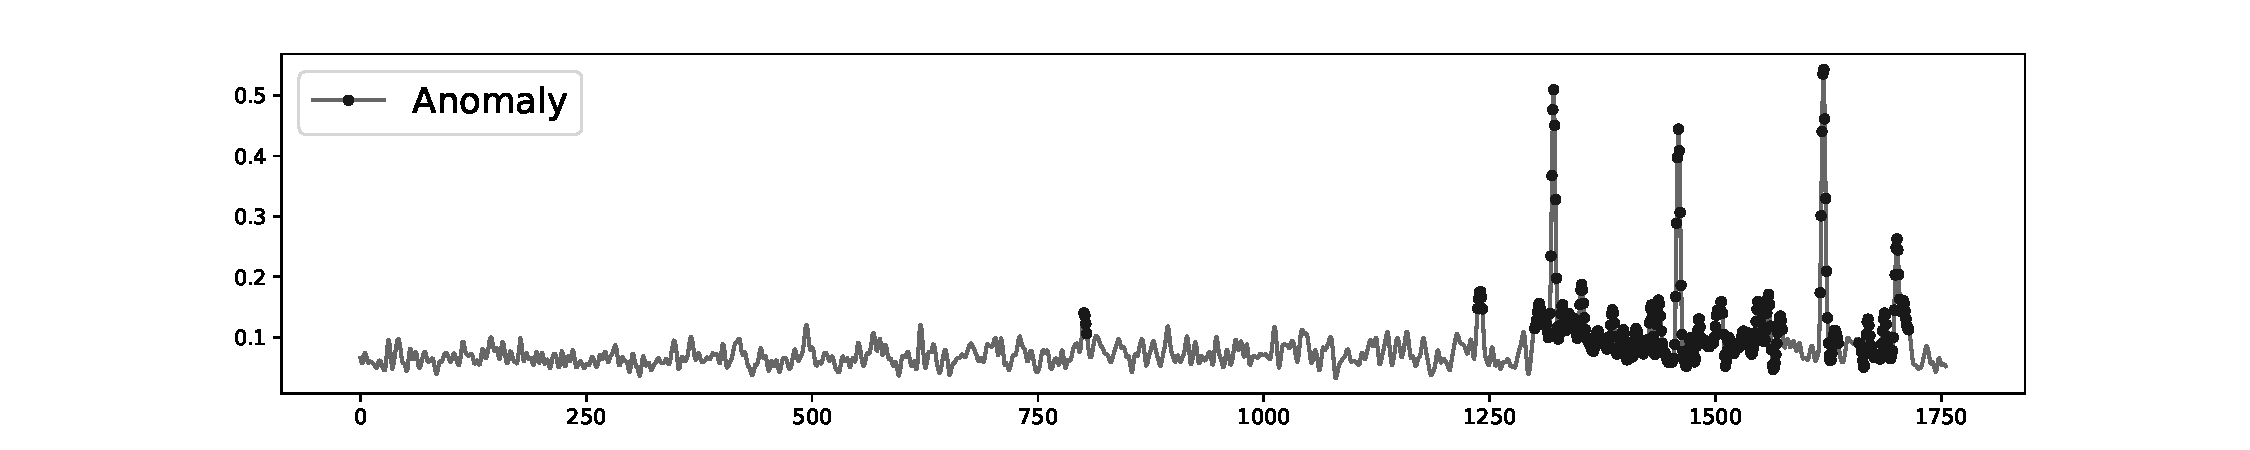
\includegraphics[width=0.48\textwidth]{gfx/chap4/scenario6.pdf}\label{scenario8}}
     \caption{Detected anomalies injected for scenarios (a) 5 and (b) 6.}
     \label{scenarios}
\end{figure*}


\begin{table}[!b]
\centering
\caption{F1 scores from production cloud metric data.}
\begin{tabular}{l|cc}
\hline
\begin{tabular}[c]{@{}l@{}}Service ID\end{tabular} & Donut & Metano \\ \hline
1                                                             & 0.72  & 0.90   \\
2                                                             & 0.26  & 0.4    \\
3                                                             & 0.67  & 0.86   \\ \hline
\end{tabular}
\label{tab:resultsproduction}
\end{table}

\begin{figure*}[!t]
     \centering
     \subfloat[][]{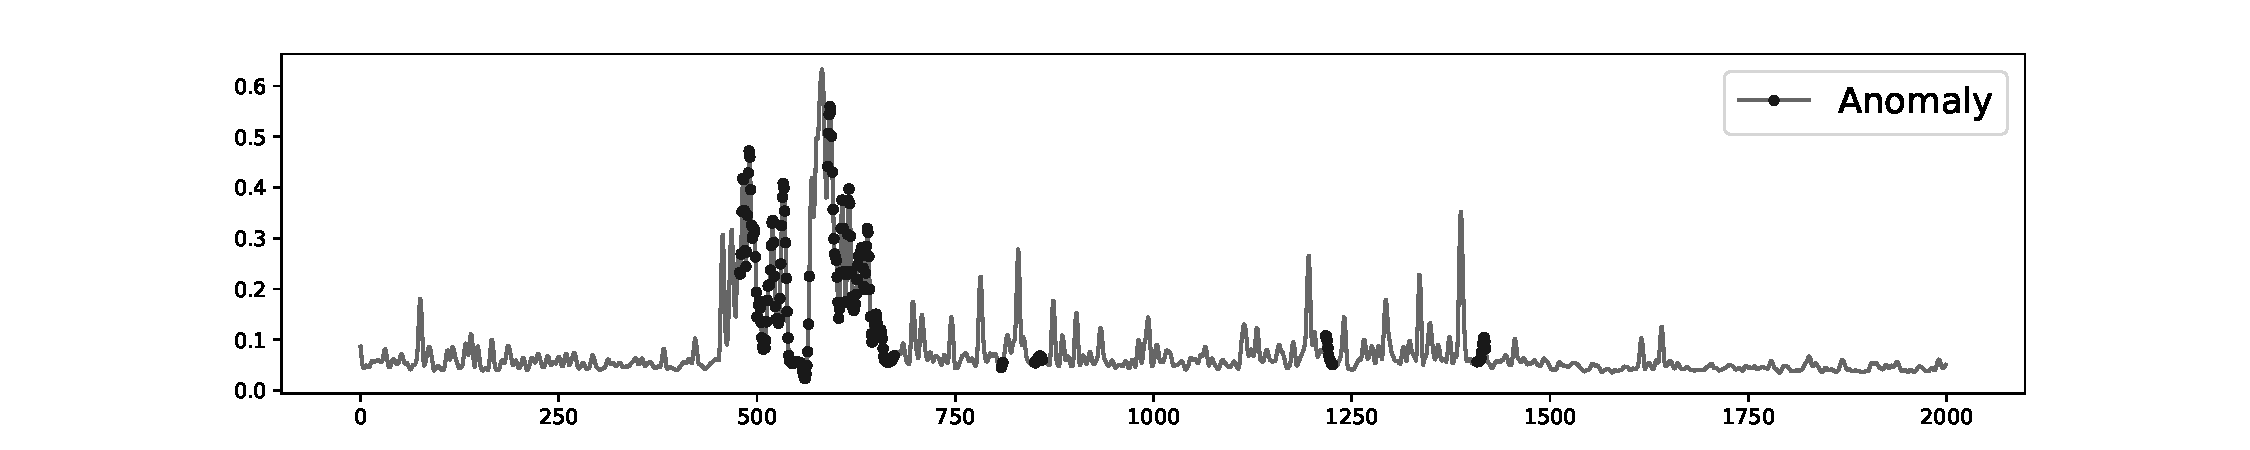
\includegraphics[width=1.0\textwidth]{gfx/chap4/donut1.pdf}\label{fig:donutresults}}
     \\
     \subfloat[][]{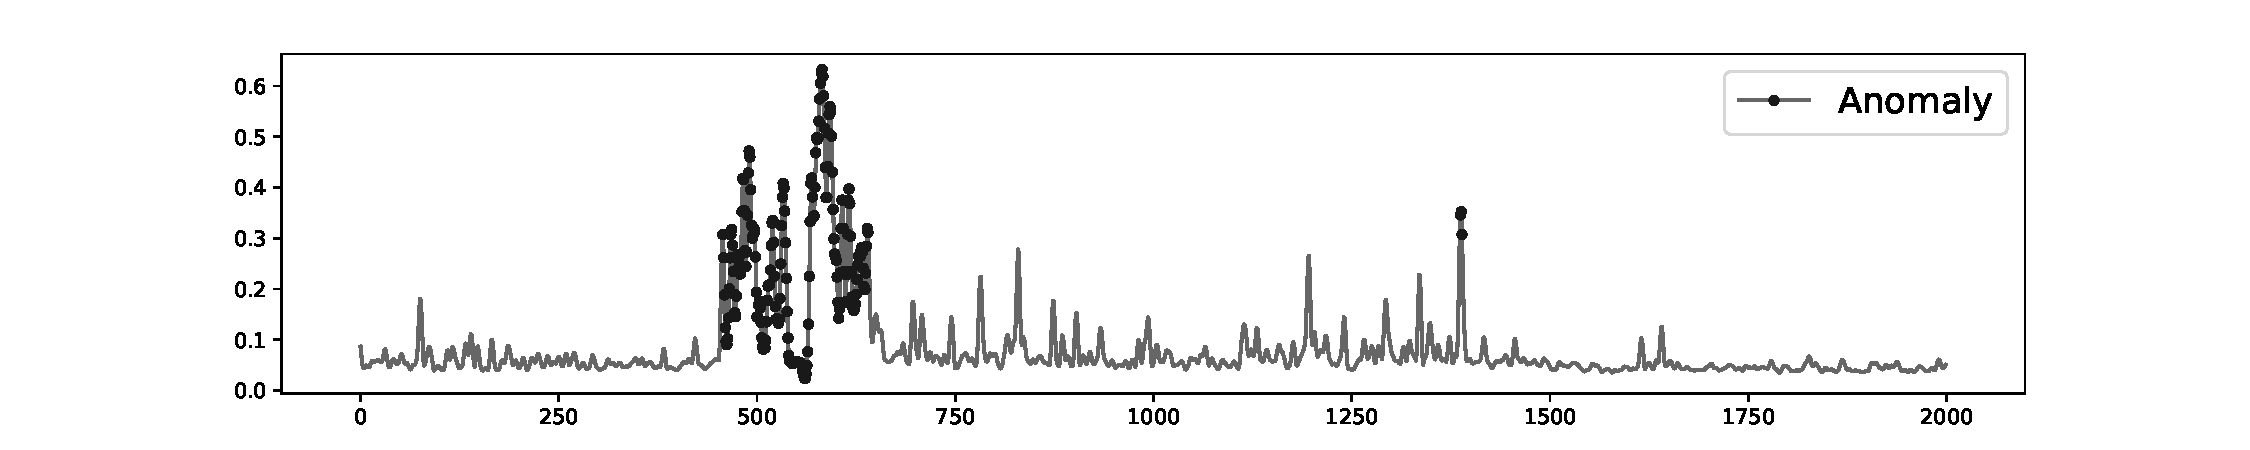
\includegraphics[width=1.0\textwidth]{gfx/chap4/vaelstm1.pdf}\label{fig:vaelstmresults}}
     \caption{Example of performed anomaly detection on the production data for one endpoint. (a) Donut, (b) Metano.}
     \label{fig:productionplotresults}
\end{figure*}

% \begin{figure*}[!t]
% \minipage{0.49\textwidth}
%   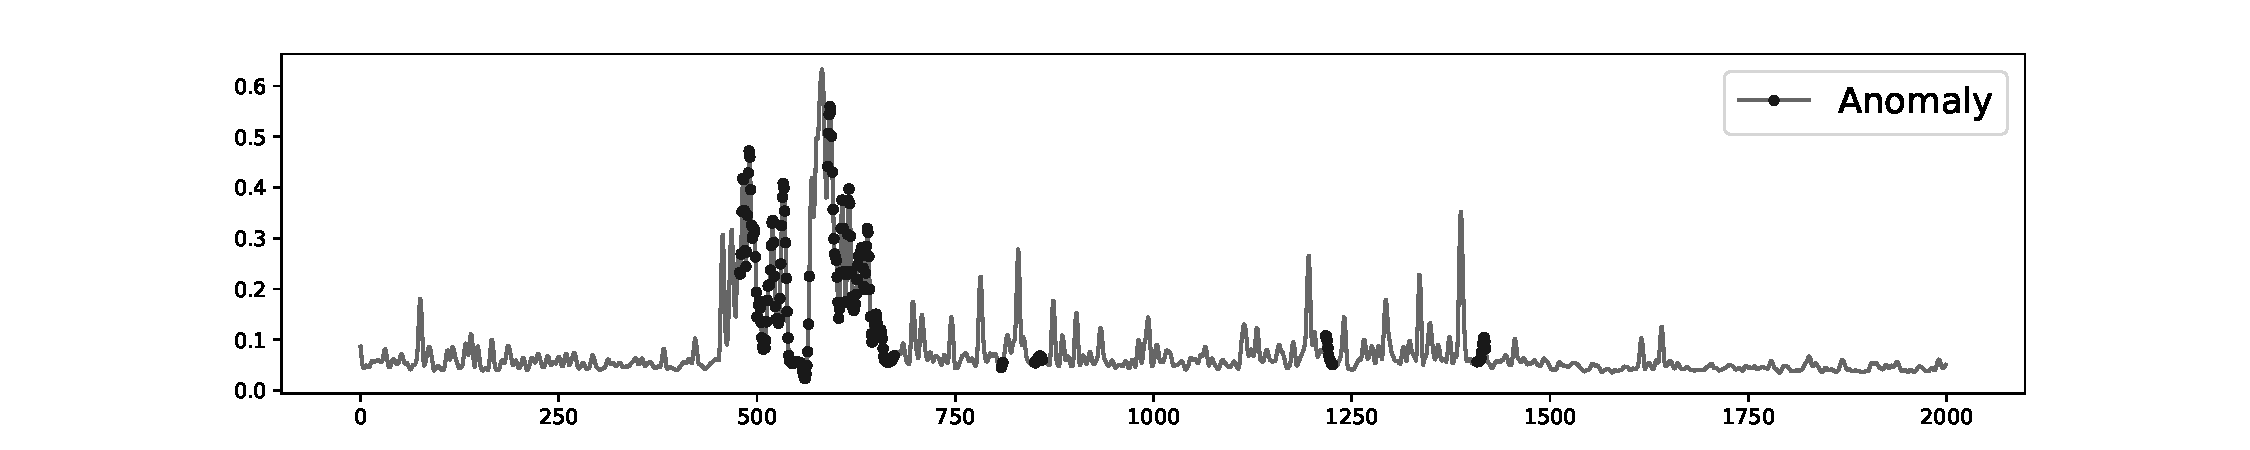
\includegraphics[width=1.0\textwidth]{gfx/chap4/donut1.pdf}\label{fig:donutresults}
% \endminipage\hfill
% \minipage{0.49\textwidth}
%   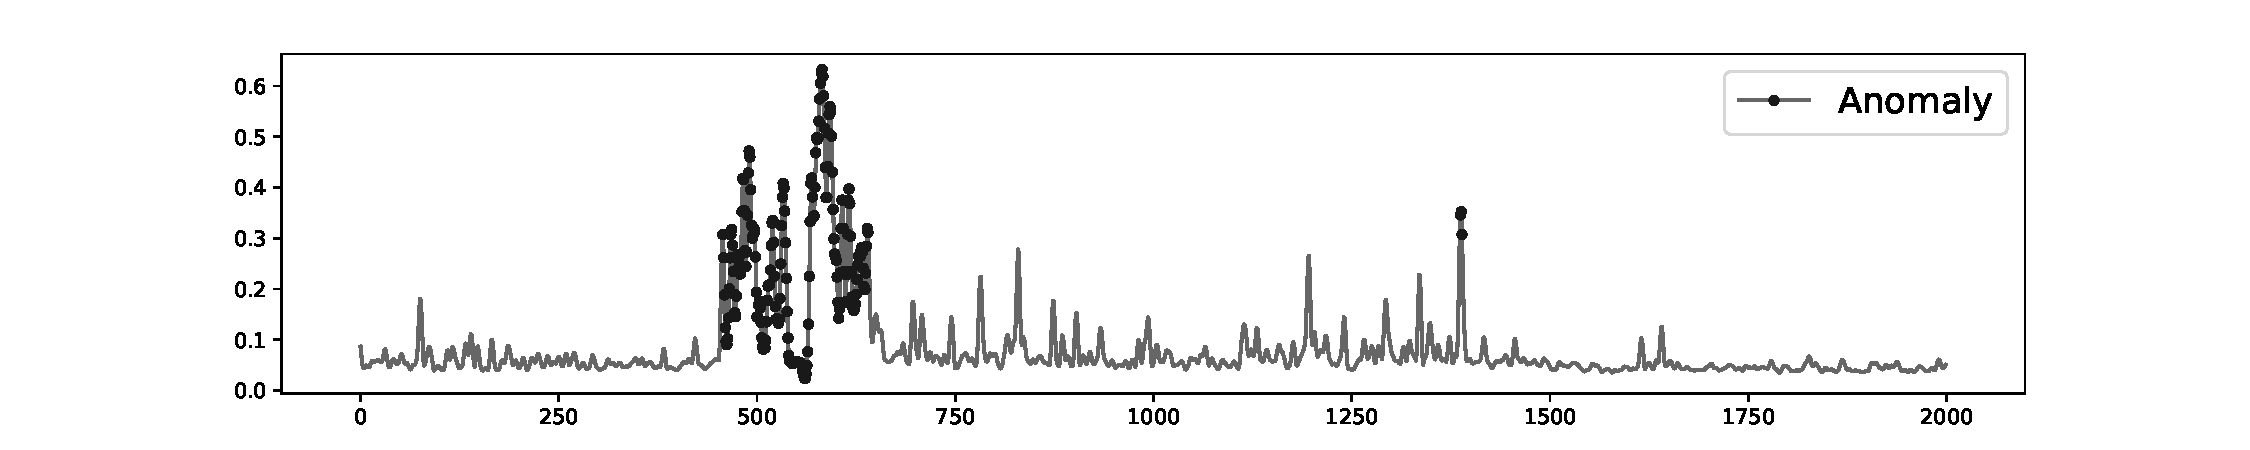
\includegraphics[width=1.0\textwidth]{gfx/chap4/vaelstm1.pdf}\label{fig:vaelstmresults}
% \endminipage
% \caption{Example of performed anomaly detection on the production data for one endpoint. (a) Donut, (b) Metano.}
% \label{fig:productionplotresults}
% \end{figure*}


\noindent\textbf{Production cloud data.} 
In the production data, in contrast to the microservice testbeds, we observed a higher noise. We show the results in Table~\ref{tab:resultsproduction}. The method has a good performance. However, decreases in the F1 scores were observed for both Metano and Donut for the production data, mainly owing to the high noise in the data. We illustrate the detection of anomalies on one production endpoint in Figure~\ref{fig:productionplotresults}. The plots show that 
Metano produces more stable predictions, while Donut has a larger number of FPs between the 750-th and 1500-th points in the time series. The analysis of the data points and method show that Metano leads to fewer FPs mainly owing to the noise handling techniques implemented in Metano, i.e., the tolerance module and increased model capacity.

\begin{figure}[!t]
\centerline{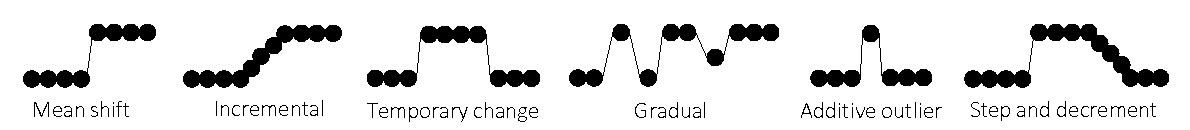
\includegraphics[width=1.0\textwidth]{gfx/chap5/patterns.pdf}}
\caption{Example of predefined patterns.}
\label{figpredefinedpatterns}
\end{figure}

Owing to the small number of production-system errors in the data, we injected several types of anomalies to further test the described method. We defined seven types of common anomalies, samples from normal distributions with different means, additive outlier, mean shift, step and decrement, incremental, temporary change, and gradual. Some of the types of anomalies are shown in Figure~\ref{figpredefinedpatterns}.

\begin{table}[htbp]
\centering
\caption{Robustness of Metano for detection of injected anomalies in production data.}
\begin{tabular}{ll}
\hline
Pattern name             &Parameters  \\ \hline
Additive\ outlier        &$RTi>0.25$   \\

Normal\_mean                          &$RTi>0.2$         \\

Temporary\ change                      &$RTi>0.25$          \\ 

Gradual                       &$RTi>0.3,\ size>10$\\ 

Mean\ shift                         &$RTi>0.2$\\

Step\ and\ decrement                      &$RTi>0.3,\ size>10$\\

Incremental                        &$RTi>0.3,\ size>10$ \\

\hline
\end{tabular}\label{tablevaeres}
\end{table}

To analyze the robustness of the algorithm, we evaluated it for several different augmentations of the original patterns, including translation, increasing the response time (e.g., $RTi=0.2$ implies setting the response time of the event to 0.2 of the maximum value), and change in the size of the anomaly (e.g., in gradual increase, $size=10$ implies that the increase from amplitude A to amplitude B is gradual over 10 events/data points). Table\ref{tablevaeres} shows the aggregated results. It summarizes the different anomaly patterns and needed minimum values for the parameters $size$ and $RTi$ that lead to detection of the corresponding anomaly type. 

\noindent\textbf{Sockshop microservice testbed.}
In this experiment, we slightly modified the input of the method to support multi-variate time series data (CPU, memory, network traffic, and response time). The method is designed for univariate time series data, as previously mentioned. However, with slight changes in the dimensionality of the input, we utilize the method to identify the root cause with anomaly detection. We computed the reconstruction errors for each of the time series.
For each fault injected in a service, we train the autoencoder with normal data and test with the anomalous data. A larger error of a particular metric compared to other metrics indicates that it has a higher probability to be the cause of the anomaly. 

Table~\ref{tabresultssockshop} shows the results of our method on different microservices and faults, in terms of precision for successfully predicting the anomaly and root cause. Our method achieve good performances in different services and faults, except for the service orders with the fault memory leak and network delay. This occurs because (1) orders is a computation-intensive service, (2) we heavily exhaust its resource memory in our fault injection, and (3) fault memory leak issues manifest as both high memory usage and high CPU usage. As our method targets the root cause, which manifests with a significant deviation in the causal metric, the accuracy decreases when the root cause manifests in multiple metrics. On average, our system achieves a precision of 94.75\%. 


\begin{table}[htbp]
\centering
\caption{Accuracy performance of Metano on Sockshop microservice testbed data.}

\begin{tabular}{lllll}
\hline
Service       & Orders & Catalogue & Carts & User \\ \hline
CPU hog       & 1.0    & 0.96      & 0.83  & 1.0  \\ 
Memory leak   & 0.66   & 1.0       & 1.0   & 1.0  \\ 
Network delay & 0.83   & 0.93      & 0.91  & 1.0  \\ \hline
\end{tabular}\label{tabresultssockshop}
\end{table}


% Further, in Figure \ref{vaeres1} and \ref{vaeres2} we visually illustrate some of the patterns detected in the series. The algorithm successfully detects the three types of anomalies injected. We note that the model was able to capture the multiple data distributions and shifts that appear early in both time series. Therefore it produced very small amount of FP.



% \begin{figure*}[htbp]
%      \centering
%      \subfloat[][]{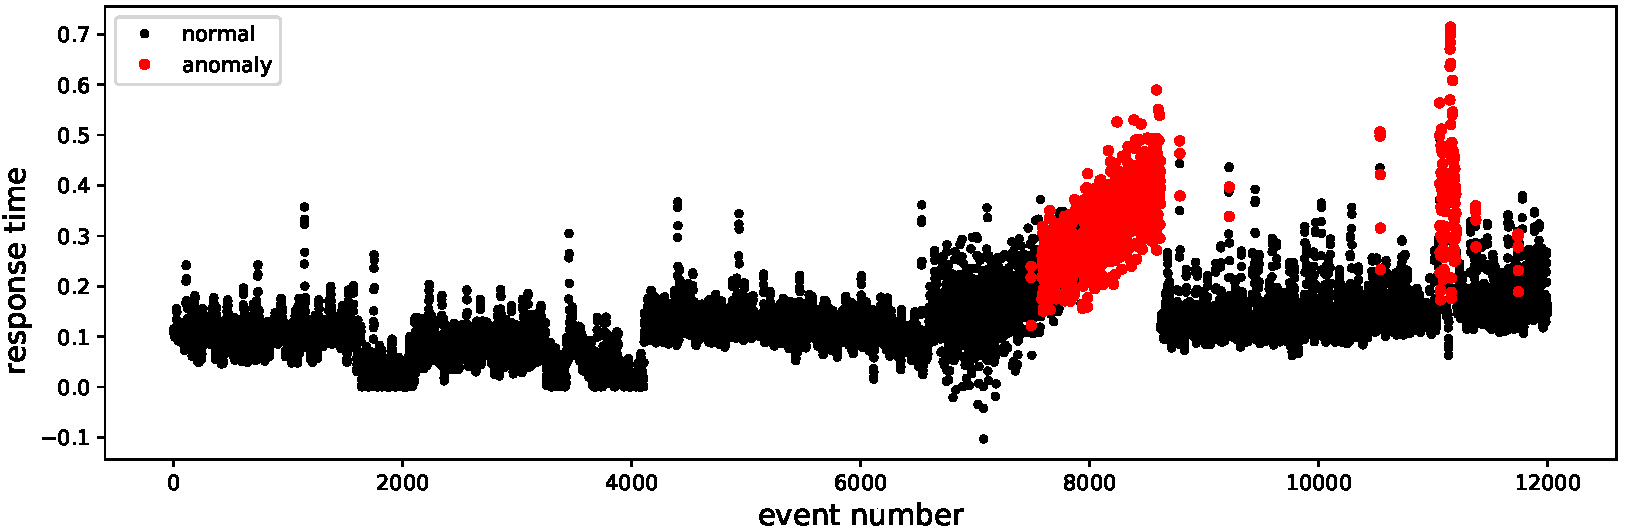
\includegraphics[width=1.0\textwidth]{gfx/chap5/vaeres1.pdf}\label{vaeres1}}
%      \\
%      \subfloat[][]{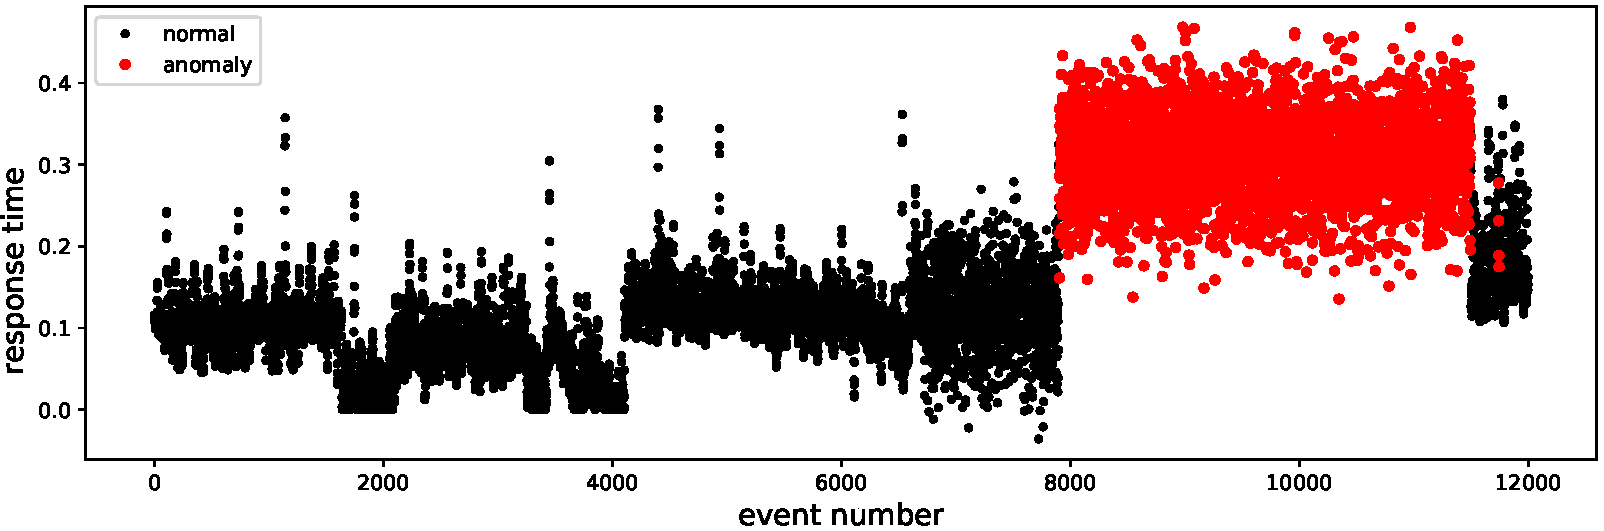
\includegraphics[width=1.0\textwidth]{gfx/chap5/vaeres2.pdf}\label{vaeres2}}
%      \caption{Example of successfully detected anomalies injected in \{host\}/ v1/\{p\_id\}/ cs/limits. Gradual and mean shift anomalies are injected in (a) and (b) respectively.}
%      \label{vaeres}
% \end{figure*}

\textbf{Faulty pattern classification}\label{resultspr}
The module can be evaluated separately from the rest of the solution, as data and predefined patterns as described. 
The dataset consists of 15 different types of patterns similar to those in Figure~\ref{figpredefinedpatterns}. In practice, the user can define patterns.

We evaluated the algorithm to analyze the performance and its limits according to the level of noise in the signal and  accuracy of classification. We achieved an accuracy of 100\% in data without additional noise and accuracies of 80\% and 48\% when Gaussian noise was added with $\sigma=0.05$ and $\sigma=0.1$, respectively. The CNN model accurately classifies the tested anomaly patterns, with an expected lower accuracy obtained in noisy patterns. For comparison, patterns recognizable by the human eye had noise levels up to approximately $\sigma=0.05$.

\subsubsection{Performance evaluation}
In large production systems, high performances of the model in training and prediction time are desirable. In this regard, we evaluate the performance of the approach. We show the results for training times in Table~\ref{perf_table1}. The training time scales linearly with the size of the time series (in number of windows). In the test-time prediction, we achieve a performance of 0.22 ms per predicted window of points (when $w=32$). The prediction times can differ with the reduction or expansion of the window size, but are still reasonably small for production usage within the limit below $10 ms$~\cite{nedelkoski2019anomaly}.

\begin{table}[htbp]
\centering
\caption{Performance evaluation of Metano in the training phase.}
\label{perf_table1}
\begin{tabular}{ ll}
\hline
\#windows  &s\\ \hline
10000	&283.9\\
5000    &148.2\\
2000	&58.56\\
1000	&31.33\\ \hline
\end{tabular}
\end{table}


\section{Related work} \label{related_work}
Anomaly detection for time series data has been extensively studied in academia and industry over the past years on different types of data. Machine learning approaches can be divided into two general categories~\cite{schmidt2018iftm}, supervised \cite{Breiman2001, joshi2001mining, joshi2002predicting, chawla2004special} and unsupervised \cite{fichtenberger2013bico,kanungo2002efficient, liu2008isolation, manevitz2001one}. The supervised methods have a limited practical usage as obtaining labels in production systems is costly and often infeasible, as described in \autoref{ch:background:sec:anomalydetection:subsec:supervised}. In the literature, the unsupervised time series anomaly detection methods are categorized into two types, deterministic and stochastic.

\textbf{Deterministic models}~\cite{malhotra2015long,filonov2016multivariate,vallis2014novel,donut,netflix,vrushali2016anomaly,Hundman:2018:DSA:3219819.3219845}. 
Several algorithms have been developed in the industry. Among them, the Netflix's robust principle component analysis (RPCA) method~\cite{netflix} and Twitter's anomaly detection~\cite{vallis2014novel}, where the underlying algorithm is referred to as seasonal hybrid ESD (S-H-ESD), which builds upon the Generalized ESD test for detecting anomalies, are most prominent. Similar ideas have been reported. For example, Vallis et al.~\cite{vallis2014novel} proposed a novel approach, based on an extreme studentized deviate (ESD) test, for detecting anomalies in long-term time series data. The approach requires detection of the trend component. Because these algorithms typically have simple assumptions for applicable metric time series (KPIs), expert's efforts need to be involved to pick a suitable detector for a given KPI, and then fine-tune the detector's parameters based on the training data. Simple ensemble of these detectors do not help much either according to~\cite{liu2015opprentice}. As a result, these detectors see only limited use in the practice. 

To address the large volumes of data produced by large systems, deep learning techniques are increasingly investigated because of their success in various domains. Malhotra et al.~\cite{malhotra2015long} used stacked recurrent hidden layers to enable learning of higher-level temporal features. They presented a model of stacked LSTM networks for anomaly detection in time series. A network was trained on nonanomalous data and used as a predictor over a number of time steps. Furthermore, Hundman et al. \cite{Hundman:2018:DSA:3219819.3219845} showed the use of LSTMs for spacecraft anomalies on telemetry data. Vrushali et al.~\cite{vrushali2016anomaly} in their paper on an anomaly-based intrusion detection system using neural networks show that these models can be used to detect various network attacks where the aim is to identify those attacks with the support of a supervised neural network. Although LSTMs-based methods can address the temporal dependence of time series, they are deterministic without stochastic variables. In our particular case, owing to the high noise they did not perform well (see~\autoref{metrics:evaluation}).

\textbf{Stochastic-based models}~\cite{fraccaro2016sequential,zong2018deep,park2018multimodal}. 
Zong et al.~\cite{zong2018deep} presented a deep autoencoding Gaussian mixture model (DAGMM) for unsupervised anomaly detection. The model utilizes a deep autoencoder to generate a low-dimensional representation and reconstruction error for each input data point, which is further fed into a Gaussian
mixture model (GMM). Instead of using decoupled two-stage training and standard expectation-maximization (EM) algorithm, DAGMM jointly optimizes the parameters of the deep autoencoder and mixture model simultaneously in an end-to-end manner, leveraging a separate estimation network to facilitate the parameter learning of the mixture model. The joint optimization, which well balances the autoencoding reconstruction, density estimation of the latent representation, and regularization, helps the autoencoder escape from less attractive local optima and further reduce the reconstruction errors, avoiding the need for pretraining. However, this method ignores the inherent temporal dependence of the time series. Previous studies suggest that, in general, stochastic variables can improve the performance of the RNN, because they can capture the probability distributions of the time series. Fraccaro et al.~\cite{fraccaro2016sequential} introduced stochastic RNNs, which combine a deterministic RNN and state space model to form a stochastic and sequential neural generative model. Xu et al. \cite{donut} showed the usability of VAEs for anomaly detection and triggering of timely troubleshooting problems on key performance indicator (KPI) data of Web applications (e.g., page views, number of online users, and number of orders). They proposed Donut, an unsupervised anomaly detection algorithm based on variational inference. Donut, at the time of evaluating Metano was considered as state-of-the-art method for anomaly detection using metric data from software systems, therefore used as a comparison method.

Compared to the above approaches, Metano is a variational RNN, which merges VAE and GRU so that the temporal dependence and stochastics of the time series can be explicitly modeled. Moreover, the inclusion of preprocessing and postprocessing with autonomous threshold selection and tolerance module improves the performance by reducing the number of false alarms. 

\section{Chapter summary}
Despite the plethora of methods and long-lasting research on time series anomaly detection, we discussed the few challenges of the task for system metric data. They include the high noise, several frequencies and distributions that reflect the normal system behavior, and recognition of patterns of anomalies.

To mitigate these challenges, we presented Metano, an approach that combines several deep learning models with pre- and postprocessing modules. We demonstrated the advantages of combining GRUs with VAEs, two deep learning models, for learning both stochastic and sequential properties of the time series data generated by distributed software systems. This is a part of the core anomaly detection model. Furthermore, we discussed the importance of the false alarm reduction logic together with the description of the recognized anomaly patterns. All proposed parts of Metano are designed to improve the administration with a small number of hyper-parameters. 
Our investigation on experimental and real-world production data showed that the approach reaches comparable to state of the art F1-scores with an average of 0.85, prediction time smaller than 10 ms, and robust classification of detected anomalies. The data were generated by two experimental microservice applications and planet-scale cloud infrastructure. Overall, we find comparable to state-of-the-art results on time series data.

Nevertheless, the largest drawback for metrics is that they contain only a limited view of the system and are system/service-scoped, which hinders the understanding except inside a particular system/service on a high level. Moreover, metrics do not provide semantic information about the anomalies, which can be found in logs and traces.
Therefore, in the next chapters, to provide a complementary and unified anomaly detection, we also analyze and present solutions in anomaly detection from log and trace data. % Chapter 4 
% Chapter X
\chapter{Anomaly Detection in Log Data} % Chapter title
\label{ch:logs} % For referencing the chapter elsewhere, use \autoref{ch:name} 
\minitoc% Creating an actual minitoc
\bigskip

\begin{figure}[!b]
\centerline{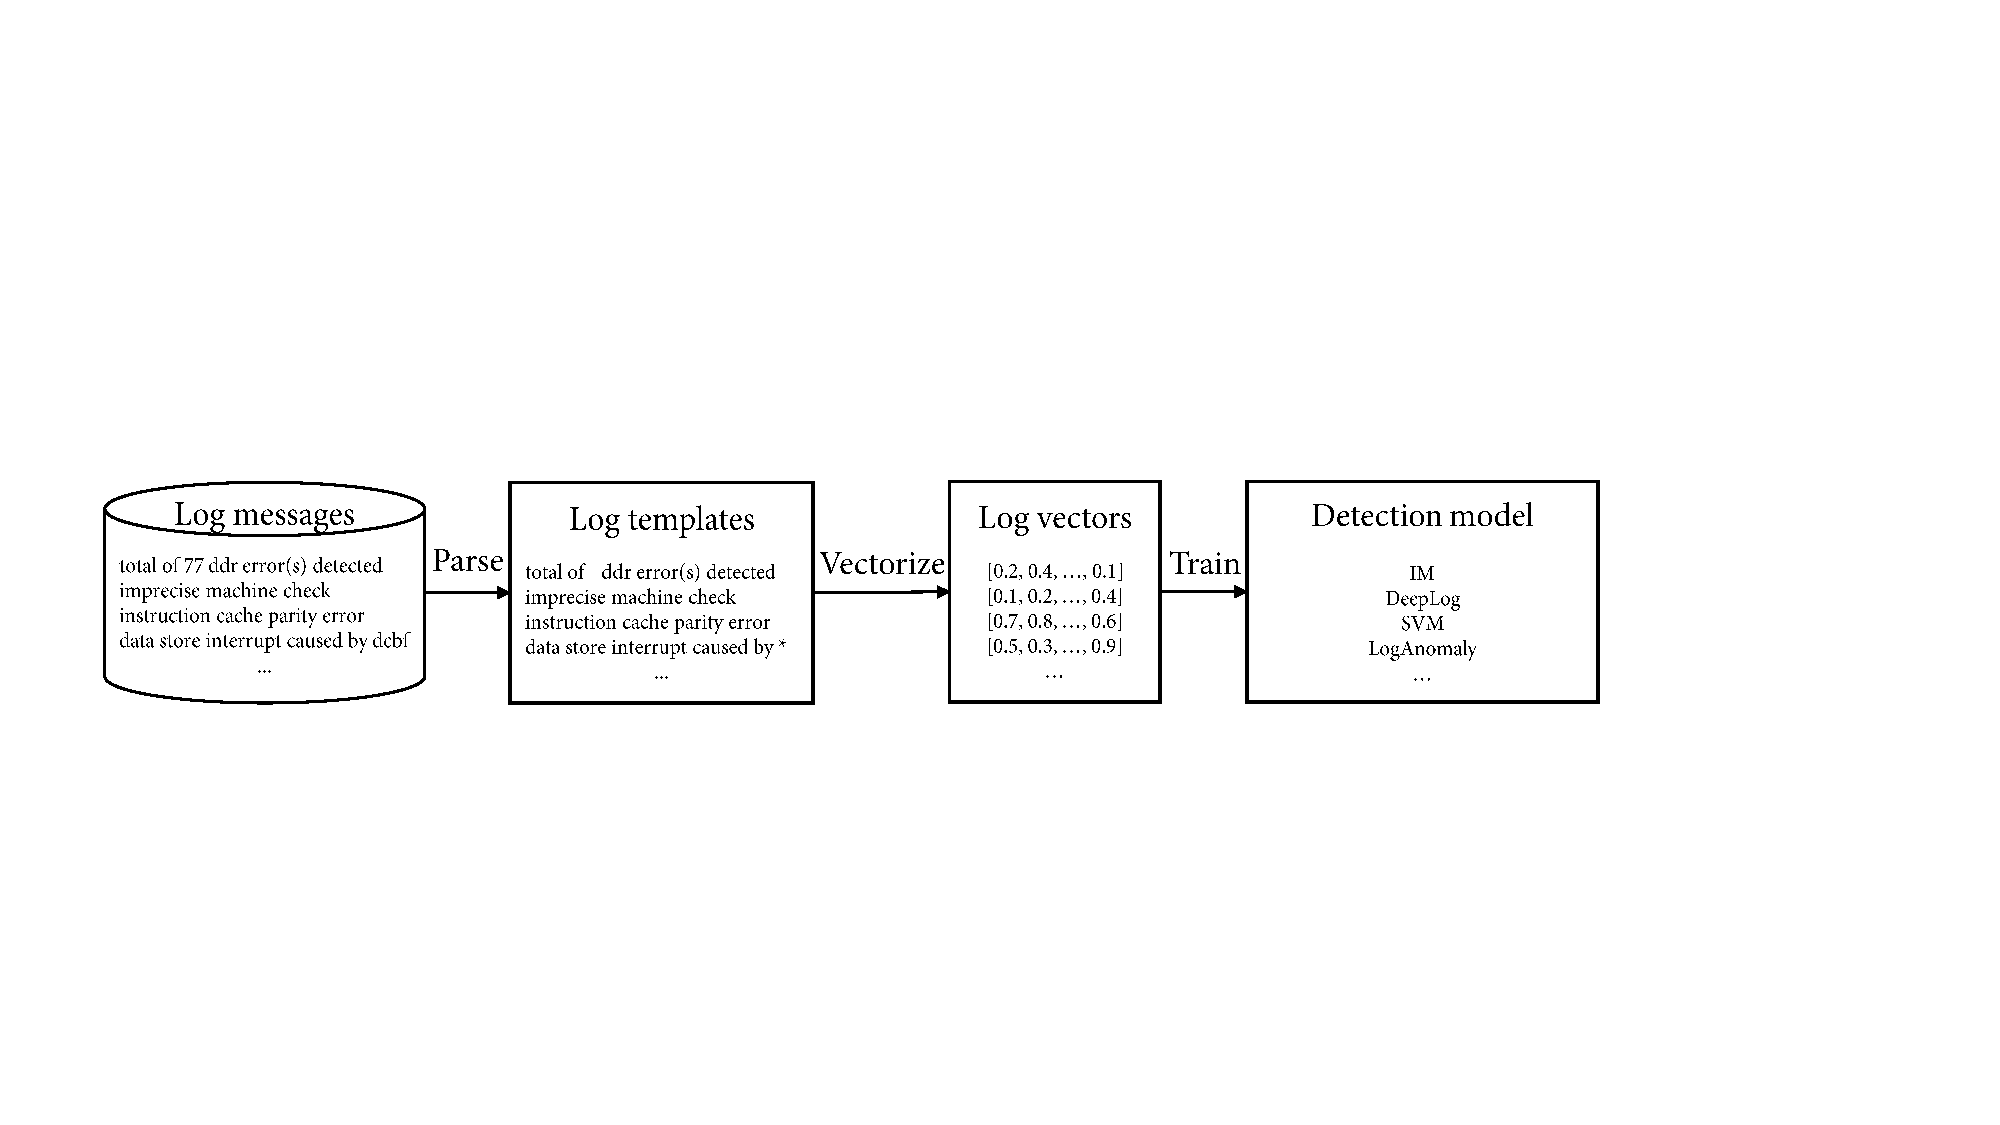
\includegraphics[width=1.0\textwidth]{gfx/chap5/traditionaloverviewlogs.pdf}}
\caption{Overview of traditional log anomaly detection approaches.}
\label{fig:parsingreferenceanomaly}
\end{figure}

In this chapter, we analyze the detection of system anomalies from log data. A plethora of methods exist to address some of the challenges posed by log data and complex systems  (~\cite{du2017deeplog,zhang2019robust,meng2019loganomaly,shilinpca}). A common characteristic is that they follow similar pipelines, depicted in Figure~\ref{fig:parsingreferenceanomaly}. (1) Owing to the unstructured nature of logs, the first crucial step is to parse log messages into structured more abstract data (e.g., templates, activities) for a subsequent analysis. (2) Vectorization of the parsed logs (i.e., the templates) is performed where they are converted into a vector form (e.g., one-hot encoding~\cite{Goodfellow-et-al-2016} or term frequency encoding~\cite{ramos2003using}). (3) The logs are utilized for training of the detection models (e.g., DeepLog~\cite{du2017deeplog}). 

The traditional log anomaly detection pipelines suggest that the log parsing, log vectorization, and detection model directly impact the effectiveness~\cite{zhu2019tools,meng2019loganomaly}.

\begin{enumerate}
    \item Even small errors, such as 4\%, in parsing could cause a performance reduction of one order of magnitude in log anomaly detection (from 40\% to 3.7\%)~\cite{he2016evaluation}.
    \item The vector representation of the log messages (log vectors) particularly affects the generalization of the models on unseen log messages, which is of importance in systems with frequent updates~\cite{zhang2019robust,meng2019loganomaly}.
    \item The models need to be sufficiently powerful and expressive to extract patterns from the potentially high-dimensional log vectors. 
\end{enumerate}

This chapter presents methods that cover these aspects in support to an effective anomaly detection.

% Therefore, first we present a novel parsing method, denoted as NuLog, which directly affects the performances of numerous methods that base their anomaly detection on the parsed log templates~\cite{du2017deeplog,meng2019loganomaly,zhang2019robust,shilinpca}. In the second part of this chapter, we present a novel log anomaly detection method, denoted as Logsy. It aims to improve the log representation, and thus the anomaly detection. In Logsy, the challenge of learning meaningful log representations is addressed directly with the optimization of novel spherical loss function. Aiming to obtain a better log representations, implicitly, we shift from the traditional anomaly detection pipeline. Logsy is able to learn the log parsing and vectorization jointly with an anomaly score in an end-to-end fashion.

We summarize the contributions in this chapter below \footnote{Parts of this chapter are published in~\cite{nedelkoski2020loganomaly,nedelkoski2020selfsupervised,nedelkoski2020data,nedelkoski2020bigdatatransfer}.}.
\begin{itemize}
    \item Novel neural log parser for log anomaly detection, denoted as NuLog~\cite{nedelkoski2020selfsupervised}, which not only parses the log messages, but also provides log vector representations.
    \item We illustrate two use cases using NuLog variants, for supervised and unsupervised anomaly detection. However, we observe a large gap between the supervised and unsupervised anomaly detection methods owing to the imperfect log representations.
    \item To bridge the gap between the supervised and unsupervised methods, we present Logsy~\cite{nedelkoski2020loganomaly}, a novel method with a spherical classification loss function for log anomaly detection.
    \item We demonstrate the key features of Logsy including utilizing log vector representations in related methods and adding expert knowledge, if available.
\end{itemize}

\section{Log parsing}\label{ch:logs:logparsing}
The content of a log record is semi-structured text, which contain tags (e.g., timestamp and service name) and free-text written by software developers. Often, the tagged data are relatively simple to parse, while the free-form text is challenging~\cite{he2017drain,zhu2019tools}. The free text is a composition of constant string templates and variable values. The template is the logging instruction (e.g., \textit{print()}, \textit{log.info()}) from which the log message is produced. The objective of a log parser is the transformation of the unstructured free text into a structured log template and associated list of variables. For example, the template \textit{"Attempting claim: memory $\langle * \rangle$ MB, disk $\langle * \rangle$ GB, vcpus $\langle * \rangle$ CPU"} is associated with the variable list \textit{["2048", "20, "1"]}, where $\langle * \rangle$ denotes the position of each variable and is connected with the positions of the values within the list. The variable list can be empty if the template does not contain variable parts. We illustrate the log parsing task in Figure~\ref{fig:log_parsing_task}.

\begin{figure}[htbp]
\centerline{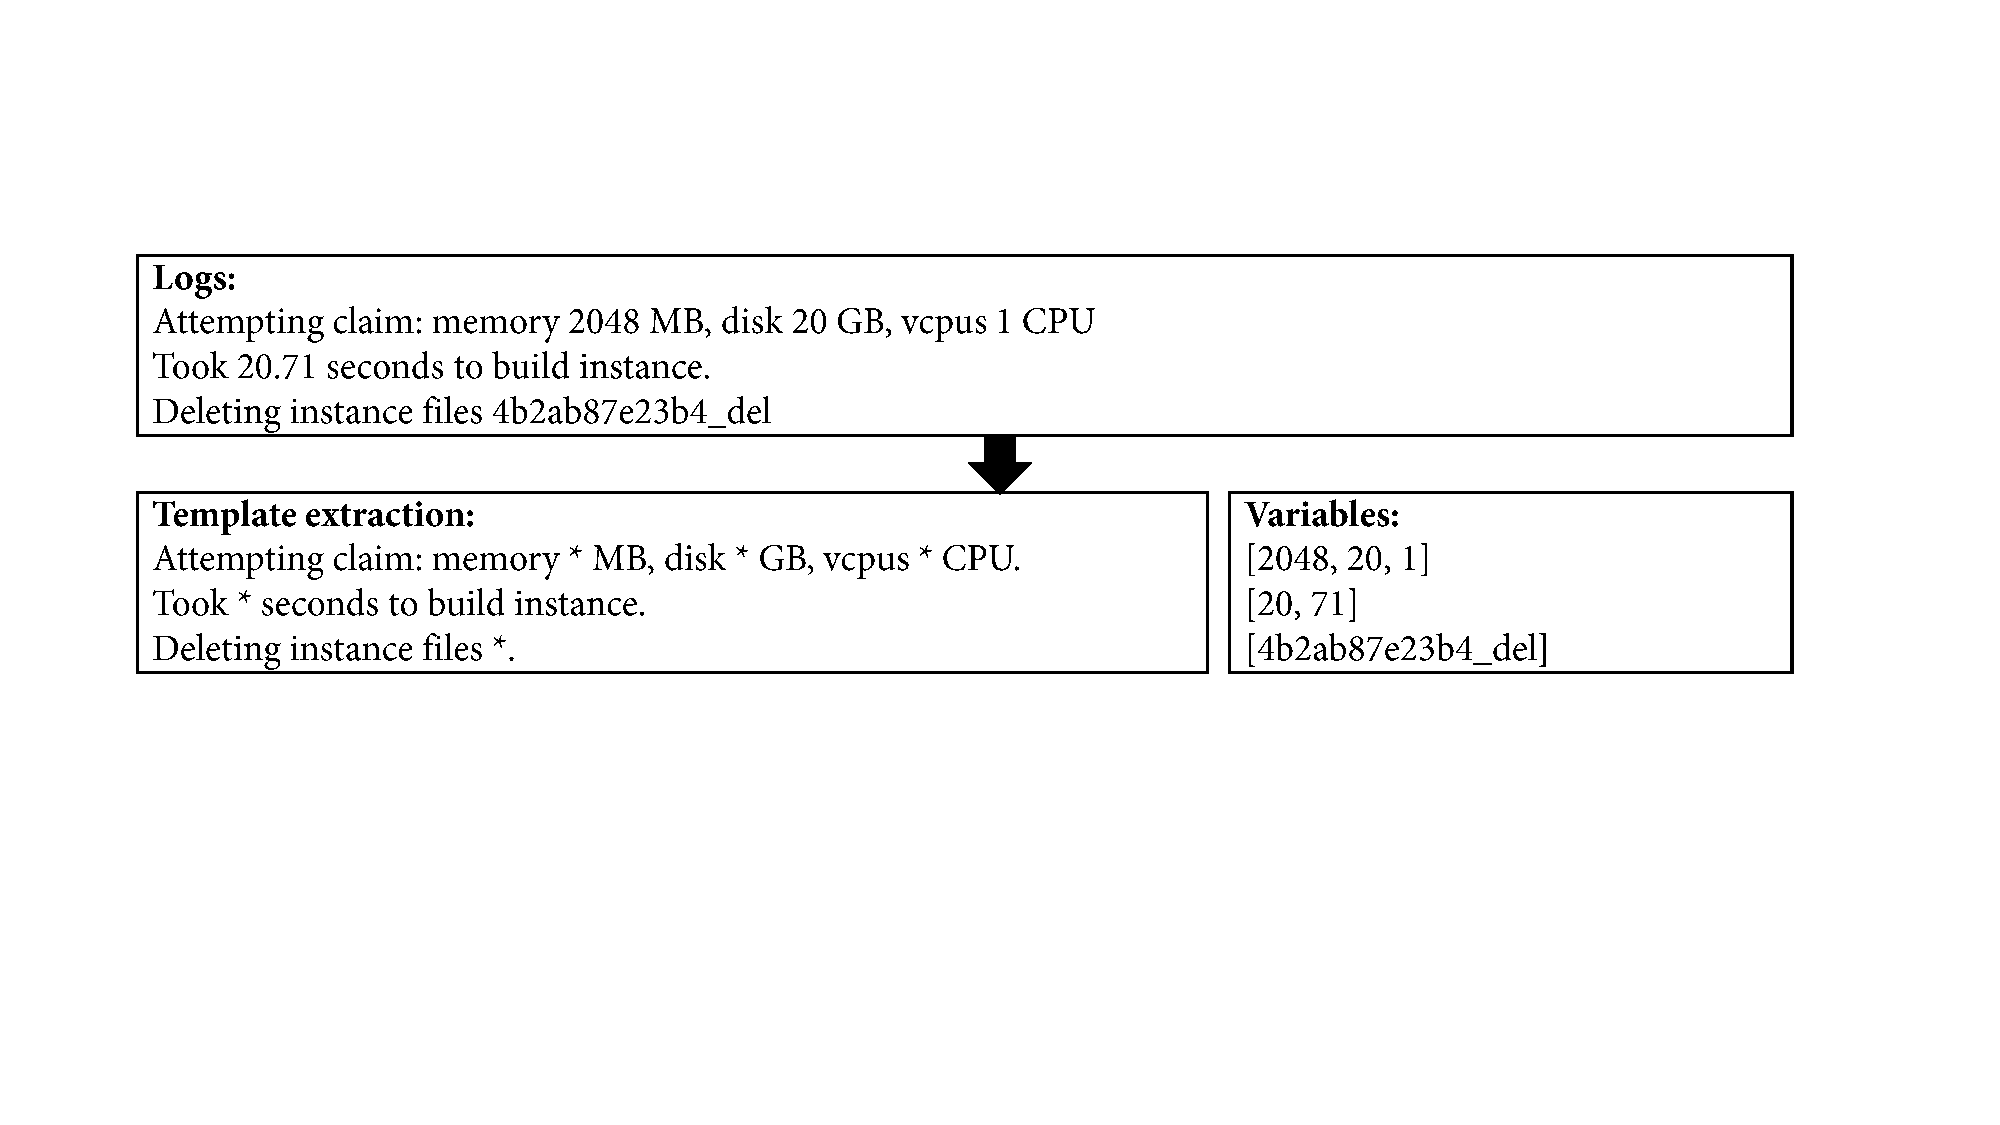
\includegraphics[width=1.0\textwidth]{gfx/chap5/log_parsing_task.pdf}}
\caption{Examples of system logs and their templates.}
\label{fig:log_parsing_task}
\end{figure}

Traditional log parsing techniques rely on regular expressions designed and maintained by human experts. This manual task is difficult to achieve in large systems consisting of diverse software and hardware components. Additionally, frequent software updates necessitate constant checking and adjustment of these statements, which is a tedious error-prone task. Related log parsing methods~\cite{he2017drain, du2016spell,hamooni2016logmine,zhu2017deep,imweber2015} depend on manual human interventions, parse trees, heuristics, and domain knowledge. Analyses of the performances of existing log parsing methods on various systems reveal their lack of robustness to produce consistently good parsing results~\cite{zhu2019tools}. 
This implies the necessity to choose a parsing method for the application or system at hand and incorporate domain-specific knowledge. In such case, operators of large distributed software systems are faced with overhead of managing different parsing methods for their components whereof each need to be accordingly understood and tuned. 

Notably, log parsing methods have to be accurate on log data from various systems, from applications on mobile operating systems to cloud infrastructure management platforms, with minimal human intervention.

After parsing, the parsed templates are transformed to log vectors for anomaly detection. The described procedures to generate log template vectors may introduce additional uncertainty and complexity. Therefore, it is desirable to incorporate the task of generating log vectors into the parsing procedure. Such a log parsing approach would meet the requirements of recent log analysis methods~\cite{meng2019loganomaly,huang2020hitanomaly,zhang2019robust}, avoid the additional external log vector generators, and provide new possibilities for log analysis tasks.

To this end, we present NuLog. We formulate the learning task on the observation that the presence of a word on a particular position in a log message is conditioned on its context. Inspired by the Cloze procedure~\cite{taylor1953cloze}, the task is carried out by masking the word that the model needs to learn to predict. In this manner, the model is forced to learn the appearance of the word within its context. The key idea for parsing is that the correct prediction of the masked word implies that the word is a part of the log template. Otherwise, it is a parameter (variable). The advantages of this approach are that it can produce both log template and numerical vector sumarization and enable downstream tasks such as anomaly detection. With the introduction of NuLog, we modify the traditional log anomaly detection pipeline illustrated in Figure~\ref{fig:parsingreferenceanomaly} to include the log parsing and vectorization within the same block. We describe NuLog in detail below.

\section{\textit{NuLog}: neural log parsing}\label{methodology}
In this section, we define the terminology, present the model, and demonstrate an approach to extract log templates and numerical log vector representations. In addition, an evaluation of the parsing method is presented.

We define a log as a sequence of temporally ordered unstructured text messages $L=(\mathbf{l_{i}} \,:\,i=1,2,...)$, where each message $\mathbf{l_{i}}$ is generated by a logging instruction within the software source code and $i$ is its positional index within the sequence. 

The smallest inseparable singleton object within a log message is token. Each log message consists of a finite sequence of tokens, $\mathbf{r_i}=(w_{j}\,:\,w \in  \mathbb{V},\,j=1,2,..., ms_i)$, where $ \mathbb{V}$ is a set (vocabulary) of all tokens, $j$ is the positional index of a token within the log message, and $ms_i$ is the total number of tokens in $\mathbf{l_i}$. We use $\vert r_i \vert$ instead of $ms_i$ in the following analysis. For different $\mathbf{l_i}$, $\vert \mathbf{r_i} \vert$ can vary. Depending on the concrete tokenization method, $w_j$ can be a word, word piece, or character. Therefore, the tokenization is defined as a transformation function $\mathcal{T}: \mathbf{l_i} \to \mathbf{r_i}, \forall i$.

The notions of context and numerical vector representation (embedding vector) are additionally introduced. For a token $w_j$, its context is defined by preceding and subsequent sequences of tokens, i.e., tuple of sequences: $C(w_j)=((w_{1}, w_{2},...,w_{j-1}), \allowbreak (w_{j+1}, w_{j+2},...,w_{\vert \mathbf{r_i} \vert}))$, where $0 \leq j \leq \vert \mathbf{r_i} \vert$. Each token is represented through an embedding vector in a $d$-dimensional space $\mathbf{x_j} \in \mathbb{R}^{d}$ of either token or log message. Therefore, we define the log message $\mathbf{x_i}=\{x_0,x_1,\dots,x_{|r_i|}\}$, where each token is represented as a vector.

\subsection{Parsing with Transformers}\label{NuLog}

NuLog is composed of preprocessing (tokenization and masking), modeling, and template extraction. The overall architecture based on an example log message input is depicted in Figure~\ref{fig:nulog}. The raw log messages are tokenized, where an \texttt{EMBEDDING} token is inserted at the first position. Using a dictionary, each token is then replaced with an index. As the last step, the masking of the tokens is performed, where the masked token is used as a target for prediction. As each token in the model is represented in vector form (indices are mapped to vectors), the \texttt{EMBEDDING} token is later used to summarize the log message from the respective token embeddings. The tokens are fed into the model, where parameters are optimized by minimizing the cross entropy loss between the target and predicted masked token. Finally, the trained model is used to extract log templates and numerical vector representation $\mathbf{z}$.

\begin{figure}[!t]
\centerline{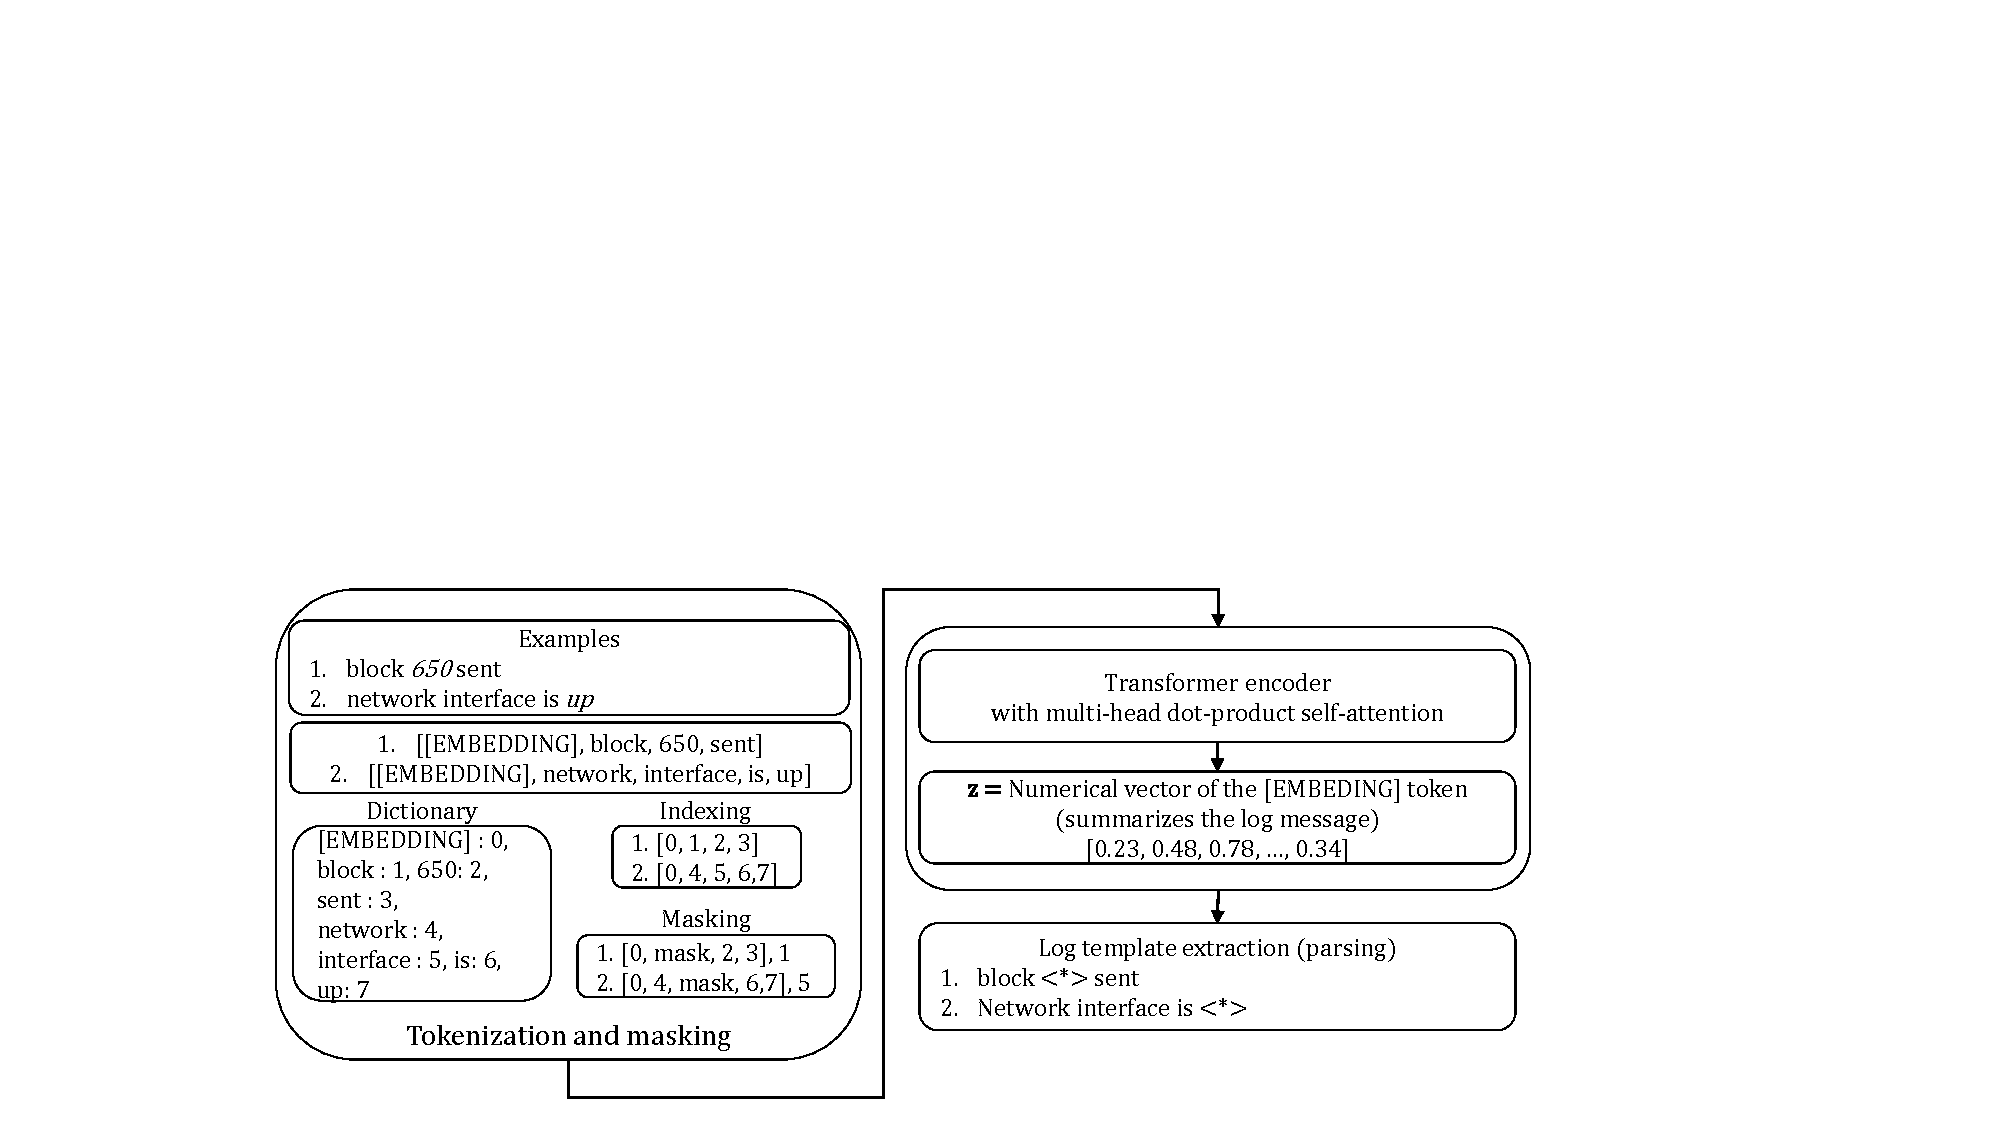
\includegraphics[width=1.0\textwidth]{gfx/chap5/nulog.pdf}}
\caption{Overview of the NuLog architecture.}
\label{fig:nulog}
\end{figure}

\textbf{Tokenization.} Tokenization transforms each log message into a sequence of tokens. For NuLog, we utilize a simple filter-based splitting criterion (e.g., on a white space) to perform a string split operation. In Figure~\ref{fig:nulog}, we illustrate the tokenization of two log messages. In contrast to related approaches~\cite{zhu2019tools} that utilize additional hand-crafted regular expressions to parse IP addresses, numbers, and URLs, NuLog does not change the original log messages at this stage. Such approaches are error-prone and require manual adjustments in different systems and updates within the same system. NuLog utilizes the appearance of the tokens within a context. These parameters (e.g., IP addresses) are assigned with a low probability as they are not constant within a particular context.

\textbf{Masking.} The concept behind the proposed parsing method is to learn a general semantic representation of the log data by analyzing occurrences of tokens within their context. We apply an approach referred to as masked language modeling (MLM). Our masking module uses the output of the tokenization step as an input, which is a token sequence of a log message. A percentage of tokens from the sequence are randomly chosen and replaced by the special \texttt{$\langle MASK \rangle$} token. If the percentage suggests replacing two tokens with masks, the masking module will create two samples, where each of the words will be masked once. In Figure~\ref{fig:nulog}, the masking is performed only on one token. Therefore, one masked log message is created. The masked token sequence is used as an input for the model, while the masked token acts as the prediction target. Furthermore, we apply padding with \texttt{PAD} tokens. The padding is applied to the maximal number of tokens across all log messages in the dataset to create evenly sized inputs.

\textbf{Model}. The method has two operation modes, offline and online. During the offline phase, log messages are used to tune all model parameters through back-propagation. During the online phase, every log message is passed forward through the model. This generates the corresponding log template and embedding vector for each log message.


\begin{figure}[!t]
\centerline{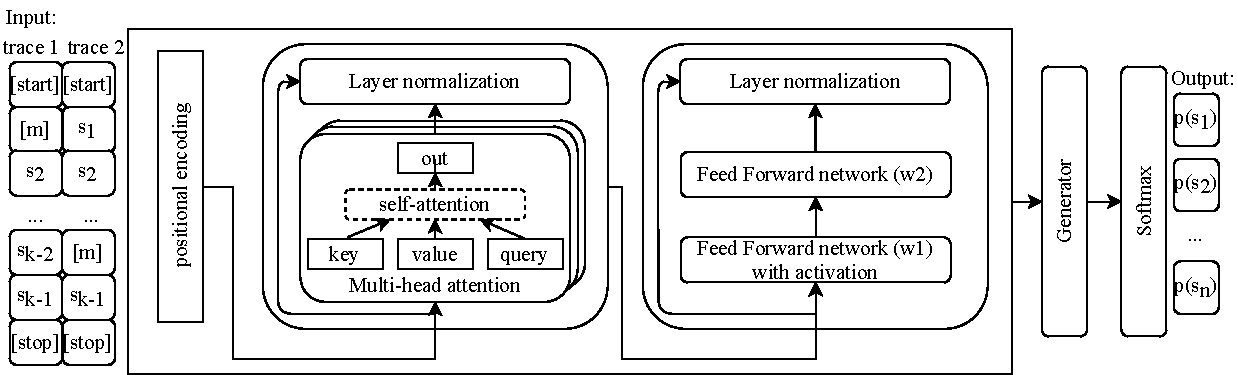
\includegraphics[width=\textwidth]{gfx/chap5/nulogtransformer.pdf}}
\caption{Model architecture of \texttt{NuLog} for parsing of the logs.}
\label{fig:2}
\end{figure}

Figure~\ref{fig:2} depicts the complete architecture. We base the model's architecture on the Transformer model~\cite{vaswani2017attention}. The Transformer network obtains word/token vectors as a weighted sum of the vectors produced by the others tokens. It attends to tokens that are similar and combines them to obtain a new representation. The model applies two operations on the input token vectors, token vectorization and positional encoding. The subsequent encoder structure uses the result of these operations as an input. It is composed of two elements, a self-attention layer and feedforward layer. The last model component is a single linear layer with a softmax activation over all tokens appearing in the logs. We provide a detailed explanation of each model element below.

As all subsequent elements of the model expect numerical inputs, we initially transform the tokens into randomly initialized numerical vectors $\mathbf{x} \in \mathbb{R}^d$. These vectors are referred to as token embeddings and are a part of the training process, which implies that they are adjusted during the training to represent the semantic meaning of tokens depending on their context. These numerical token embeddings are passed to the positional encoding block. In contrast to, e.g., recurrent architectures, attention-based models do not contain any notion of input order. Therefore, this information needs to be explicitly encoded and merged with the input vectors to consider their position within the log message. This block calculates a vector $\mathbf{p} \in \mathbb{R}^d$ representing the relative position of a token based on sine and cosine functions,
%We follow the recommendations of~\cite{vaswani2017attention} and employ the following equations for positional embeddings calculation

\begin{equation}\label{eq:sincosin}
    p_{2k}=sin \left( \frac{j}{10000^{\frac{2k}{v}}} \right), \;\;
    p_{2k+1}=cos \left( \frac{j}{10000^{\frac{2k + 1}{v}}} \right),
\end{equation}

where $k=0,1,\dots,d-1$ is the index of each element in $\mathbf{p}$ and $j=1,2,\dots,M$ is the positional index of each token. The parameter $k$ describes the exponential relationship between each value of vector $\mathbf{p}$. Additionally, sine and cosine functions are interchangeably applied. Both enable a better discrimination of the respective values within a specific vector of $\mathbf{p}$. Furthermore, both functions approximately linearly depended on the position parameter $j$, which was hypothesized so that the model can easily attend at the respective positions. Finally, both vectors can be combined as $\mathbf{x'} = \mathbf{x} + \mathbf{p}$. The values for the frequency of the sine and cosine functions were obtained empirically, as in ~\cite{vaswani2017attention}.

The encoder block of our model starts with a multi-head attention element, where a softmax distribution over the token embeddings is calculated. Intuitively, it describes the significance of each embedding vector for the prediction of the target masked token. We summarize all token embedding vectors as rows of a matrix $X'$ and apply the following formula,
\begin{equation}
    X''_l=softmax \left( \frac{Q_l \times K^T_l}{\sqrt{w}} \right) \times V_l, \; \text{for} \; l = 1, 2, \dots, L,
\end{equation}
where $L$ denotes the number of attention heads, $w = \frac{d}{L}$, and $d \, \text{mod} \, L = 0$. The parameters $Q$, $K$, and $V$ are matrices, which correspond to the query, key, and value elements in Figure~\ref{fig:2}, respectively. They are obtained by applying matrix multiplications between the input $X'$ and respective learnable weight matrices $W_{l}^{Q}$, $W_{l}^{K}$, $W_{l}^{V}$,

\begin{equation}
    Q_l= X' \times W_{l}^{Q}, \; K_l= X' \times W_{l}^{K}, \; V_l= X' \times W_{l}^{V},
\end{equation}

where $W_{l}^{Q}, \; W_{l}^{K}, \; W_{l}^{V} \in \mathbb{R}^{M \times w}$. The division by $\sqrt{w}$ stabilizes the gradients during the training~\cite{vaswani2017attention}. The softmax function is then applied and the result is used to scale each token embedding vector $V_{l}$. The scaled matrices $X''_l$ are concatenated to a single matrix $X''$ with a size of $M \times d$. As depicted in Figure~\ref{fig:2}, a residual connection between the input token matrix $X'$ and its respective attention transformation $X''$ exists, followed by a normalization layer $norm$. These are used to improve the performance of the model by addressing different potential problems during the learning such as small gradients and covariate shift phenomena. In this manner, the original input is updated by the attention-transformed equivalent, $X' = norm(X' + X'')$.

The last element of the encoder consists of two feed-forward linear layers with a ReLU activation between them. It is applied individually on each row of $X'$. Thereby, identical weights for every row are used, which can be described as a convolution over each attention-transformed matrix row with a kernel size of one. This step serves as an additional information enrichment for the embeddings. A residual connection followed by a normalization layer between the input matrix and output of both layers is employed. This model element preserves the dimensionality $X'$.

The final element of the model consists of a single linear layer. It receives the encoder result $X'$ and extracts the token embedding vector of the \texttt{EMBEDDING} token. As every log message token sequence is prepadded by this special token, it is the first row of the matrix, i.e., $\mathbf{x'_0} \in X'$. The linear layer maps this vector with a size of $d$ to a vector whose size corresponds to the total number of tokens $|\mathbb{T}|$ in the dataset. The subsequent softmax is utilized to calculate the probability distribution over each element of $\mathbb{T}$. During the training with a cross-entropy loss function, the masked token is used as the target to be predicted. As the last vector embedding of the \texttt{EMBEDDING} token is used for prediction, it summarizes the log message. We hypothesize that the constant part of log templates will constraint the model to learn similar \texttt{EMBEDDING} vectors when log messages are from the same template. This leads to mapping of the log messages to their vector representation, which can enable other downstream log analysis tasks.

\newpage

\subsection{Log template and vector extraction}
After the model is trained, the extraction of all log templates within a log dataset is executed online. Each log message is used as an input and the masking module is configured such that every token is masked consecutively, one at a time. We measure the model's ability to predict each token, and thus decide whether the token is a constant part of the template or variable. A high confidence in the prediction of a specific token indicates a constant part of the template. A low confidence is interpreted as a variable. We employed the following procedure. If the prediction of a particular token is in the top $\epsilon$ predictions and does not contain numbers, we consider it a constant part of the template; otherwise, we considered it a variable. For each variable, an indicator \texttt{$\langle * \rangle$} is placed on its position within the log message.

Once the templates are obtained, to perform anomaly detection, we follow the traditional log anomaly detection pipeline described above.

% The computational complexity for parsing one log message $\mathbf{t_i}$ is $\mathcal{O}(\text{max}_{i}|\mathbf{t_i}|)$ + $\mathcal{O}(\text{max}_{i}|\mathbf{t_i}|)$ + $\mathcal{O}(1)$ + $\mathcal{O}(|\mathbb{T}|\log \mathbb{T})$, for tokenization, masking, forward pass, and top-k sorting, where $\text{max}_{i}|\mathbf{t_i}|$ is the maximum number of tokens in the log messages and $|\mathbb{T}|$ is the size of the set of all tokens. This makes our method in worst case $\mathcal{O}(|\mathbb{T}|\log \mathbb{T})$

Another contribution of NuLog is that we enable generation of a vector representation of the log messages. The~\texttt{EMBEDDING} token attends over all tokens in the log. Hence, it embeds information of all of them without being biased toward any of the original log tokens. Moreover, it encodes semantic information inside the logs. This leads to one-to-one mapping between the log message type and vector representation of the \texttt{EMBEDDING} token. 

\subsection{NuLog: Evaluation}\label{nulog:evaluation}
To quantify the effectiveness of \texttt{NuLog} in the task of log parsing, we evaluate it on 10 presented datasets and compare it to 12 existing log parsing methods. We reproduce the results of the parsing benchmark~\cite{zhu2019tools} for all log parsers and include NuLog's results. All parsers and their parameters are tuned to achieve their best performances.

% \begin{table}[!t]
% \centering
% \caption{Datasets and \texttt{NuLog} hyperparameter setting.}
% % \resizebox{\columnwidth}{!}{%
% \begin{tabular}{llcc}
% \hline
% System   & T   & epochs & $\epsilon$   \\ \hline
% BGL      &120 & 3        & 50  \\
% Android  &166  & 5        & 25  \\
% OpenStack&43  & 6        & 5   \\
% HDFS     &14  & 5        & 15  \\
% Apache   &6  & 5        & 12  \\
% HPC      &46 & 3        & 10  \\
% Windows  &50  & 5        & 95  \\
% HealthApp&75  & 5        & 100 \\
% Mac      &341 & 10       & 300 \\
% Spark    &36  & 3        & 50  \\ \hline
% \end{tabular}
% % }
% \label{table:hyperparameters}
% \end{table}

\subsubsection{Datasets}\label{Datasets}
The log datasets employed in our experiments consist of: (1) supercomputer logs, Blue Gene L (BGL) and HPC, (2) distributed system logs, Hadoop distributed file system (HDFS), OpenStack, and Spark, and (3) standalone software logs, Apache, Windows, Mac, and Android. To enable reproducibility, we follow the guidelines of Zhu et al.~\cite{zhu2019tools} and utilize a random sample of 2000 log messages from each dataset, where the ground truth templates are available. 

\subsubsection{Evaluation metrics}
For comparability of NuLog to the previous methods~\cite{zhu2019tools}, we utilize the benchmark PA metric. It is defined as the ratio of correctly parsed log messages to the total number of log messages. A log message is considered correctly parsed if its log template corresponds to the same group of log messages as that of the ground truth. For example, if a log sequence $[e_1, e_2, e_2]$ is parsed to $[e_1, e_4, e_5]$, we obtain $PA=\frac{1}{3}$ as the second and third messages are not grouped together. The parsing accuracy does not measure the string matching between the template and ground truth. Therefore, we enrich the evaluation with an additional metric, the edit distance. This can be used to quantify the dissimilarity between two log templates by counting the minimum number of operations required to transform one into the other.




\begin{table}[htbp]
\centering
\caption{Comparisons of log parsers and our method \texttt{NuLog} in terms of PA.}
\resizebox{\columnwidth}{!}{%
\begin{tabular}{|l|cccccccccccccc|}
\hline
Dataset   & SLCT           & AEL            & LKE   & LFA            & LogSig & SHISHO & LogCluster & LenMa & LogMine        & Spell          & Drain          & MoLFI & BoA          & NuLog           \\ \hline 
HDFS      & 0.545          & 0.998          & 1.000 & 0.885          & 0.850  & 0.998  & 0.546      & 0.998 & 0.851          & 1.000          & 0.998          & 0.998 & \textbf{1.000} & 0.998          \\
Spark     & 0.685          & 0.905          & 0.634 & \textbf{0.994} & 0.544  & 0.906  & 0.799      & 0.884 & 0.576          & 0.905          & 0.920          & 0.418 & 0.994          & \textbf{1.000} \\
OpenStack & \textbf{0.867} & 0.758          & 0.787 & 0.200          & 0.200  & 0.722  & 0.696      & 0.743 & 0.743          & 0.764          & 0.733          & 0.213 & 0.867          & \textbf{0.990} \\
BGL       & 0.573          & 0.758          & 0.128 & 0.854          & 0.227  & 0.711  & 0.835      & 0.690 & 0.723          & 0.787          & \textbf{0.963} & 0.960 & 0.963          & \textbf{0.980} \\
HPC       & 0.839          & \textbf{0.903} & 0.574 & 0.817          & 0.354  & 0.325  & 0.788      & 0.830 & 0.784          & 0.654          & 0.887          & 0.824 & 0.903          & \textbf{0.945} \\
Windows   & 0.697          & 0.690          & 0.990 & 0.588          & 0.689  & 0.701  & 0.713      & 0.566 & 0.993          & 0.989          & \textbf{0.997} & 0.406 & 0.997          & \textbf{0.998} \\
Mac       & 0.558          & 0.764          & 0.369 & 0.599          & 0.478  & 0.595  & 0.604      & 0.698 & \textbf{0.872} & 0.757          & 0.787          & 0.636 & \textbf{0.872} & 0.821          \\
Android   & 0.882          & 0.682          & 0.909 & 0.616          & 0.548  & 0.585  & 0.798      & 0.880 & 0.504          & \textbf{0.919} & 0.911          & 0.788 & \textbf{0.919} & 0.827          \\
HealthApp & 0.331          & 0.568          & 0.592 & 0.549          & 0.235  & 0.397  & 0.531      & 0.174 & 0.684          & 0.639          & \textbf{0.780} & 0.440 & 0.780          & \textbf{0.875} \\
Apache    & 0.731          & 1.000          & 1.000 & 1.000          & 1.000  & 1.000  & 0.709      & 1.000 & 1.000          & 1.000          & 1.000          & 1.000 & \textbf{1.000} & \textbf{1.000} \\ \hline
\end{tabular}
}
\label{table:comparisonPA}
\end{table}



\subsubsection{Parsing results}

\textbf{Parsing accuracy} results are presented in Table~\ref{table:comparisonPA}. Each row contains the datasets while the compared methods are presented in the table columns. The penultimate column contains the highest value of the first twelve columns, referred to as best of all, while the last column contains the results for \texttt{NuLog}. The values in bold indicate the best of the methods per dataset. HDFS and Apache datasets are most frequently parsed with a PA of 100\%, because HDFS and Apache error logs have relatively unambiguous event templates, which are simple to identify. For them, \texttt{NuLog} achieves comparable results. For the Spark, BGL, and Windows datasets, the existing methods already achieve high PA values above 96\% (BGL) or above 99\% (Spark and Windows). Our method can slightly outperform these methods. For the rather complex log data from OpenStack, HPC, and HealthApp, the baseline methods achieve a PA between 78\% and 90\%, which are significantly outperformed by \texttt{NuLog} by 4--13\%.

With the proposed method, we explicitly aim to support a broad range of diverse log data types. Therefore, the robustness of \texttt{NuLog} is analyzed and compared to those of the related methods. Figure~\ref{robustness_pa} shows the accuracy distribution of each log parser across the log datasets within a boxplot. From left to right in the figure, the log parsers are arranged in ascending order of the median PA. LogSig has the lowest, while \texttt{NuLog} has the highest median PA. Although most log parsing methods achieve high PA values of 90\% for specific log datasets, they have large variances when applied across all given log types. \texttt{NuLog} outperforms the other baseline methods in terms of PA robustness with a median of 0.99, which is even above the best of all medians of 0.94.

\begin{figure}[!t]
\centerline{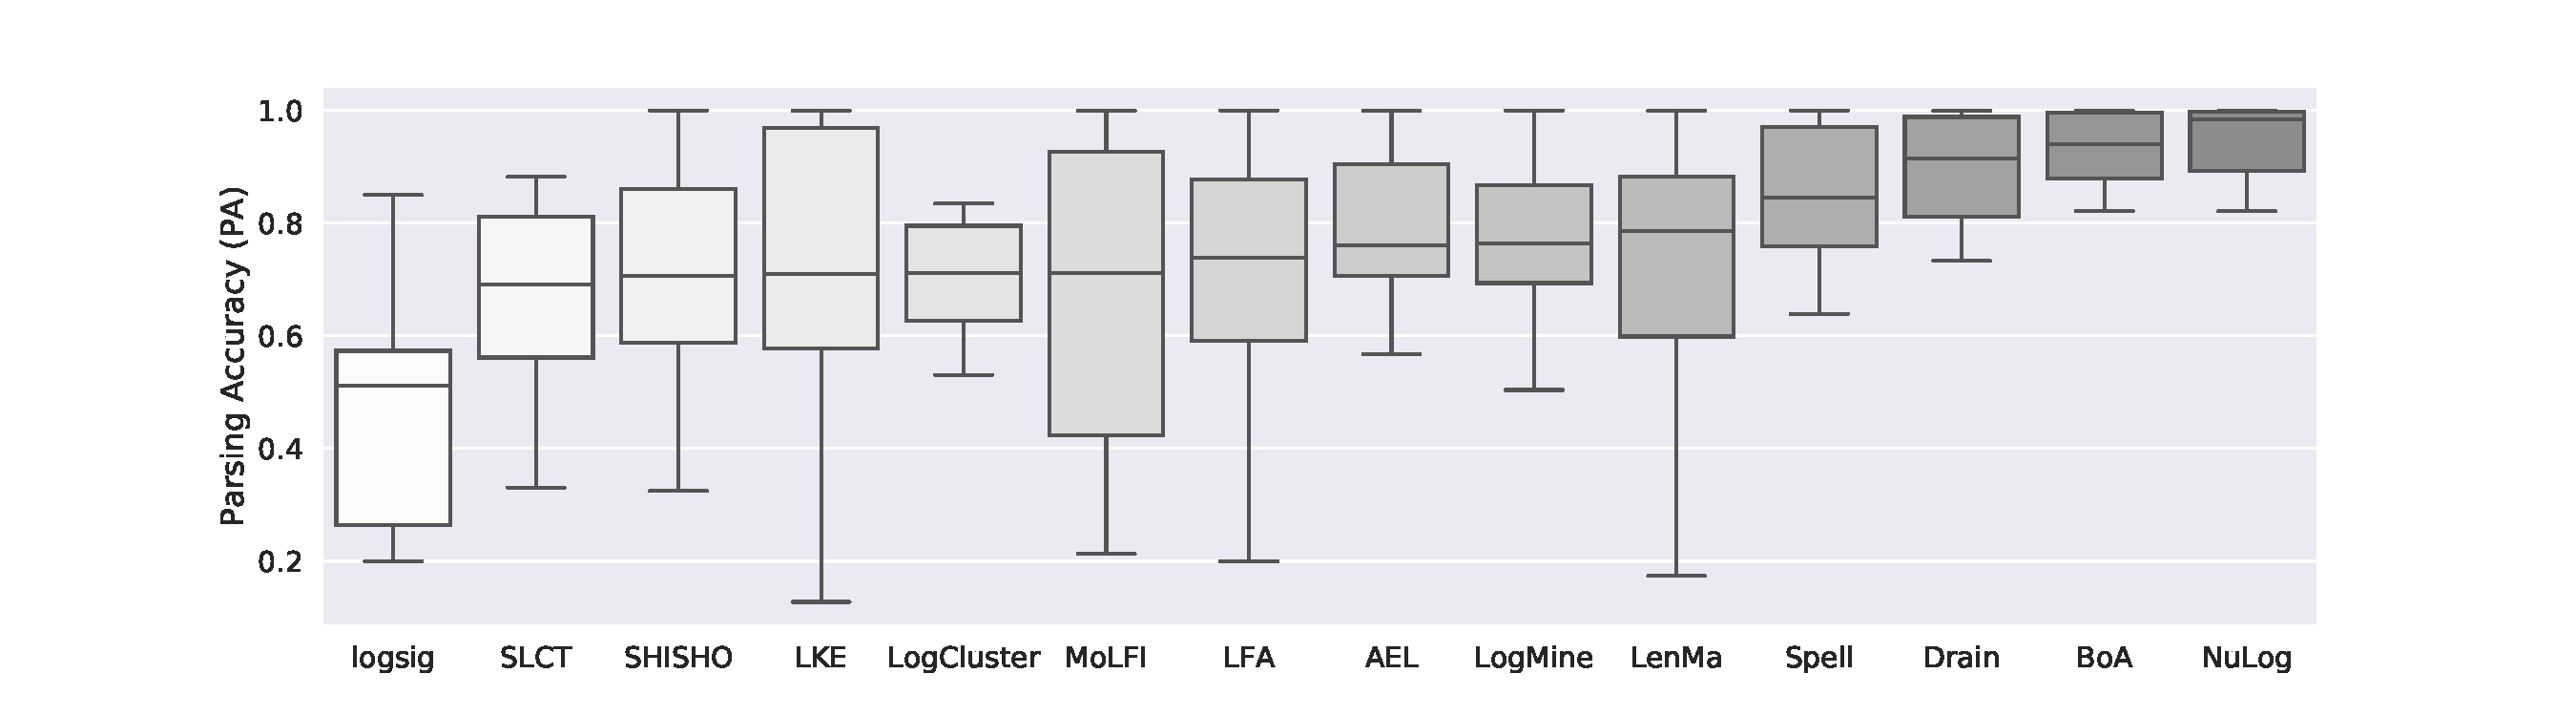
\includegraphics[width=1.0\textwidth]{gfx/chap4/robustness.pdf}}
\caption{Robustness evaluation of the PA of the log parsers.}
\label{robustness_pa}
\end{figure}

\begin{table}[!htbp]
\centering
\caption{Comparisons of log parsers and our method \texttt{NuLog} in terms of edit distance.}
\resizebox{\columnwidth}{!}{%
\begin{tabular}{|l|cccccccccccccc|}
\hline
Dataset &  LogSig &      LKE &    MoLFI &     SLCT &      LFA &  LogCluster &   SHISHO &  LogMine &    LenMa &    Spell &      AEL &    Drain  &  BoA&    NuLog \\
\hline 
HDFS & 19.1595 &  17.9405 &  19.8430 &  13.6410 &  30.8190 &     28.3405 &  10.1145 &  16.2495 &  10.7620 &   9.2740 &   8.8200 &   8.8195 &    8.8195& \textbf{3.2040} \\
Spark & 13.0615 &  41.9175 &  14.1880 &   6.0275 &   9.1785 &     17.0820 &   7.9100 &  16.0040 &  10.9450 &   6.1290 &   3.8610 &   \textbf{3.5325} &  3.5325&  12.0800 \\
BGL &  11.5420 &  12.5820 &  10.9250 &   9.8410 &  12.5240 &     12.9550 &   8.6305 &  19.2710 &   8.3730 &   7.9005 &   5.0140 &   \textbf{4.9295} &   4.9295&  5.5230 \\
HPC &  4.4475 &   7.6490 &   3.8710 &   2.6250 &   3.1825 &      3.5795 &   7.8535 &   3.2185 &   2.9055 &   5.1290 &   \textbf{1.4050} &   2.0155 &   1.4050&      2.9595 \\
Windows &  7.6645 &  11.8335 &  14.1630 &   7.0065 &  10.2385 &      6.9670 &   5.6245 &   6.9190 &  20.6615 &   4.4055 &  11.9750 &   6.1720 &   5.6245&     \textbf{4.4860} \\
Android & 16.9295 &  12.3505 &  39.2700 &   3.7580 &   9.9980 &     16.4175 &  10.1505 &  22.5325 &   3.2555 &   8.6680 &   6.6550 &   3.2210 &    3.2210&    \textbf{1.1905} \\
HealthApp & 17.1120 &  14.6675 &  21.6485 &  16.2365 &  20.2740 &     16.8455 &  24.4310 &  19.5045 &  16.5390 &   8.5345 &  19.0870 &  18.4965 &    14.6675&  \textbf{6.2075} \\
Apache & 14.4420 &  14.7115 &  18.4410 &  11.0260 &  10.3675 &     16.2765 &  12.4405 &  10.2655 &  13.5520 &  10.2335 &  10.2175 &  \textbf{10.2175} &   10.2175& 11.6915 \\
OpenStack & 21.8810 &  29.1730 &  67.8850 &  20.9855 &  28.1385 &     31.4860 &  18.5820 &  23.9795 &  18.5350 &  27.9840 &  \textbf{17.1425} &  28.3855 &   17.1425&  21.2605 \\
Mac & 27.9230 &  79.6790 &  28.7160 &  34.5600 &  41.8040 &     21.3275 &  19.8105 &  17.0620 &  19.9835 &  22.5930 &  19.5340 &  19.8815 &      17.062& \textbf{2.8920} \\
\hline
\end{tabular}
}

\label{table:edit_distance}
\end{table}


\textbf{Edit distance} scores are listed in Table~\ref{table:edit_distance}. The table structure is the same as that of the PA results. The value in bold indicates the best edit distance across all tested methods per dataset. In terms of edit distance, \texttt{NuLog} outperforms the existing methods on the HDFS, Windows, Android, HealthApp, and Mac datasets. Its performance is comparable on the BGL, HPC, Apache, and OpenStack datasets. It achieves a larger edit distance on the Spark log data.

We verify the robustness in terms of edit distance across the different log datasets. Figure~\ref{robustness_ed} shows a box-plot of the edit distance distribution of each log parser for all log datasets. From left to right in the figure, the log parsing methods are arranged in descending order of the median edit distance. Again, although most log parsing methods achieve minimal edit distance scores under 10, most of them have large variances over different datasets and are thus not generally applicable for diverse log data types. MoLFI has the largest median edit distance, while Spell and Drain exhibit small median edit distances for multiple datasets. NuLog outperforms the state-of-the-art models, with the smallest edit distance values with a median of 5.00, which is smaller than the best-of-all median of 7.22.

These results show that NuLog parses the log messages accurately, while preserving the string structure of the message.


\begin{figure}[!htbp]
\centerline{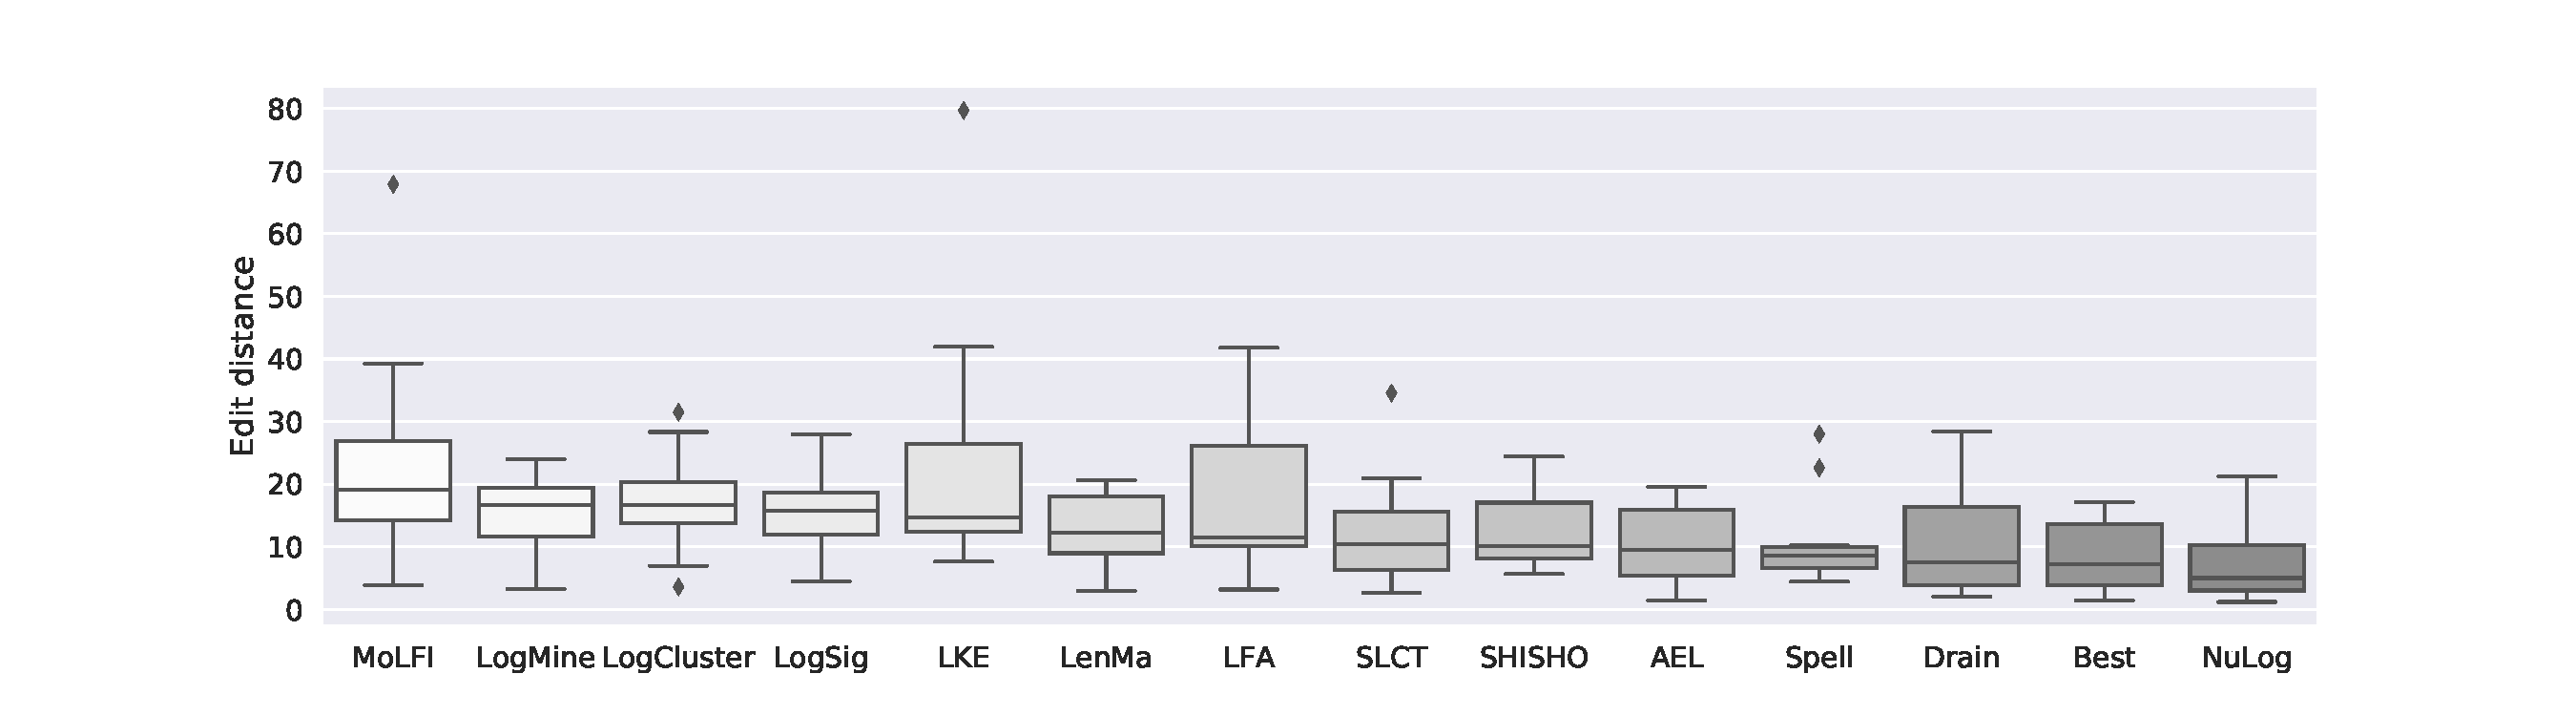
\includegraphics[width=1.0\textwidth]{gfx/chap4/robustness_ed.pdf}}
\caption{Robustness evaluation of the edit distance of the log parsers.}
\label{robustness_ed}
\end{figure}

\newpage 

\section{From log representations to log anomaly detection}
The improvement in the log parsing has a large impact on the subsequent log anomaly detection task in the traditional pipeline for a log analysis~\cite{zhu2019tools}. As described above, the next step in the log anomaly detection pipeline is to obtain log vectors. In previous unsupervised approaches, the log vectors are obtained by one-hot encoding of the templates or combination of word vectors using, e.g., word2vec~\cite{mikolov2013distributed}. In NuLog, these log vectors were directly produced together with the parsed log template. 
\begin{figure}[!b]
\centerline{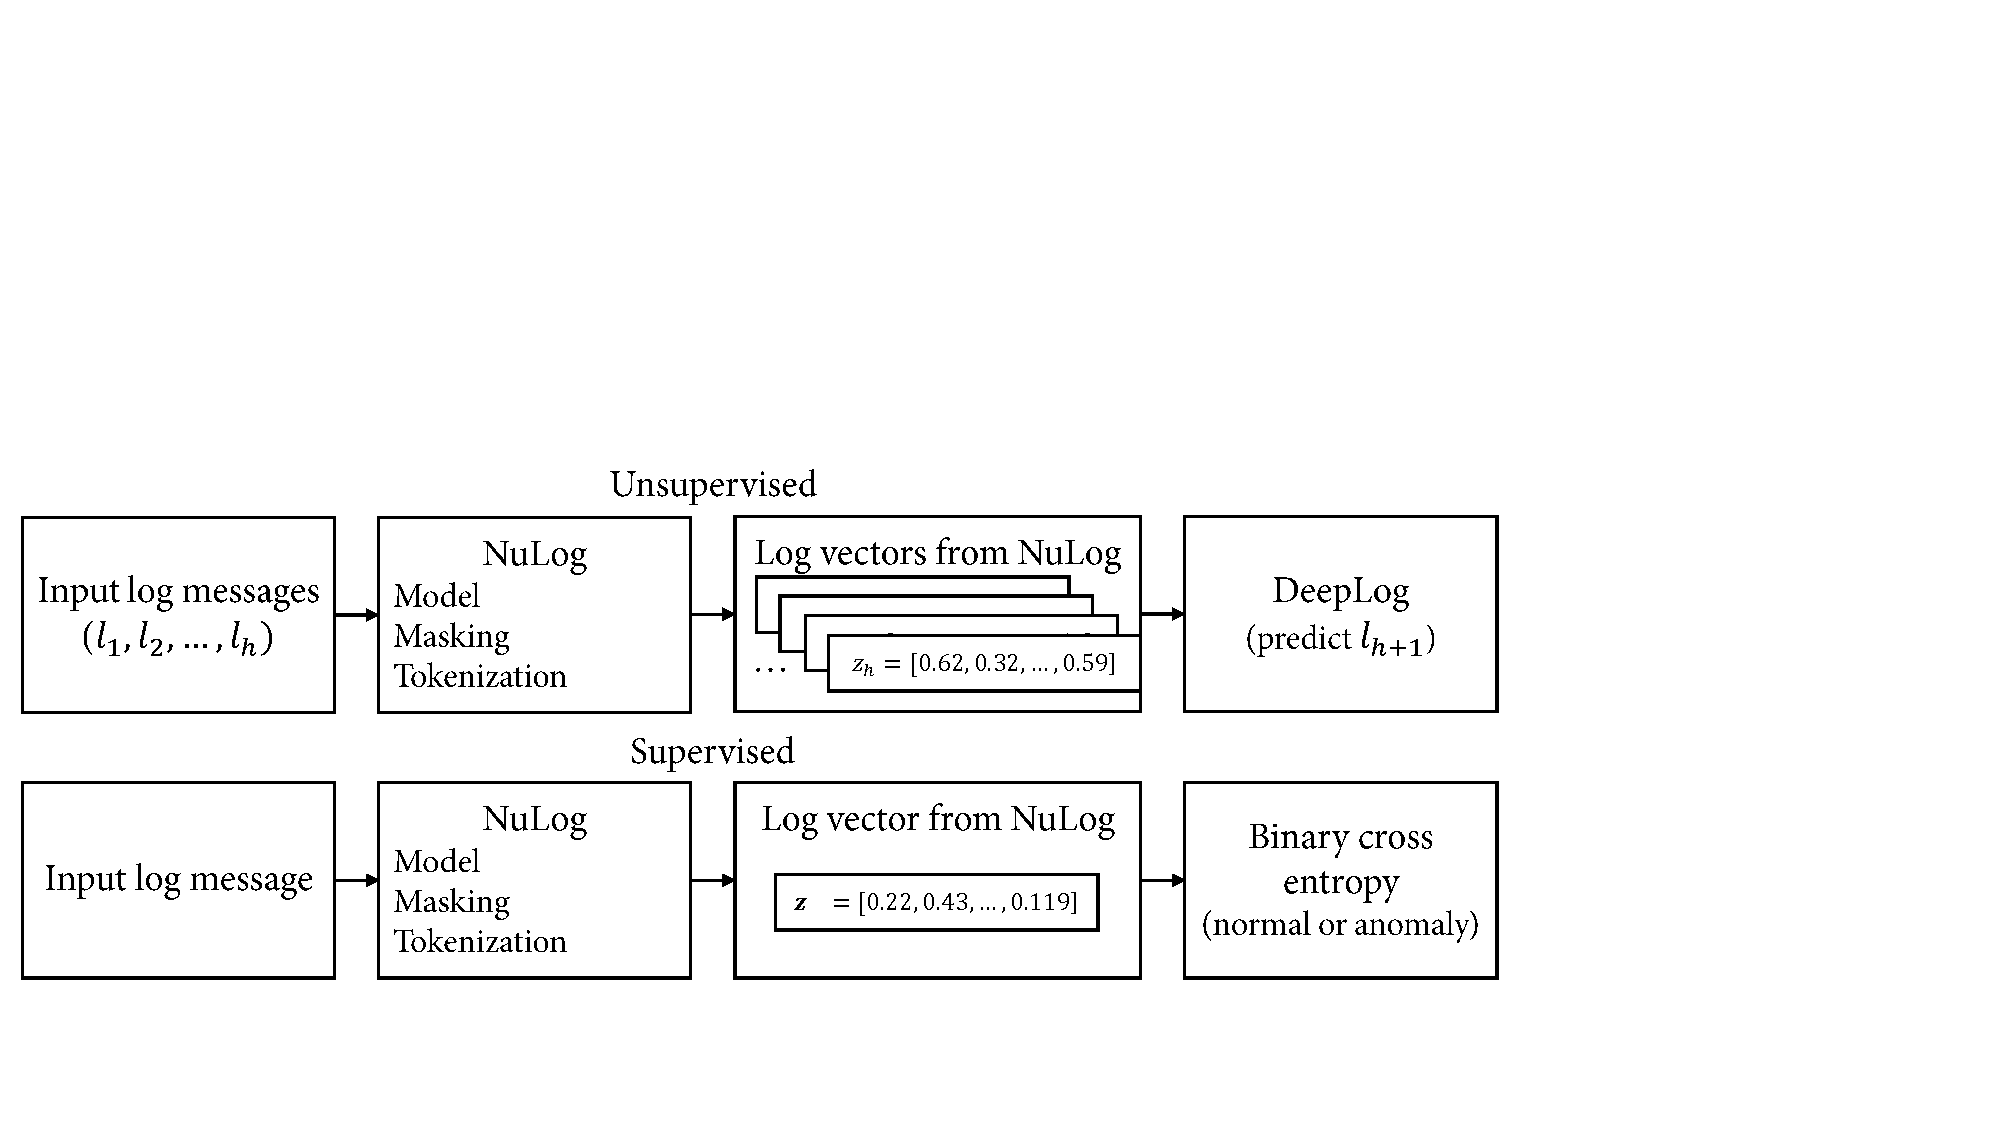
\includegraphics[width=1.0\textwidth]{gfx/chap5/nulogdeeplog.pdf}}
\caption{Unsupervised (top) and supervised (bottom) methods for downstream anomaly detection.}
\label{fig:downstream}
\end{figure}

We perform an additional analysis to compare the performances of (1) one-hot encoding of the templates, as they are utilized in the state-of-the-art log anomaly detection method, DeepLog~\cite{du2017deeplog}, (2) DeepLog with log vectors obtained from NuLog, instead of one-hot encoding, and (3) NuLog with an additional layer to perform supervised log anomaly detection.




We depict the unsupervised anomaly detection use case of NuLog in Figure~\ref{fig:downstream}. The log vectors from NuLog obtained from the ~\texttt{EMBEDDING} token are utilized by the modified DeepLog method instead of one-hot encoding to perform anomaly detection. DeepLog requires a sequence of $h$ log messages and learns to predict the next log message. If it successfully predicts the next log message, the message is classified as normal; otherwise, it is classified as an anomaly. 

In the supervised case, we learn the log message embeddings in a supervised manner. First, NuLog is trained on the parsing task. Second, we replace the last softmax layer by a linear layer, which maps the \texttt{EMBEDDING} vector to 0 or 1 (normal or anomaly), i.e., optimizes the model's parameters, as well as the log representations (the \texttt{EMBEDDING} vector) to perform binary classification. 


\begin{table}[htbp]
\centering
\caption{Scores for the anomaly detection use cases.}
\begin{tabular}{l|cc}
\hline
Method                     & \begin{tabular}[c]{@{}c@{}}BGL 10\%\\ 80\%-20\% train-test\end{tabular} & \begin{tabular}[c]{@{}c@{}}BGL 100\%\\ 80\%-20\% train-test\end{tabular} \\ \hline
DeepLog                    & 0.24                                                                    & 0.18                                                                     \\
DeepLog with NuLog vectors & 0.99                                                                    & 0.28                                                                     \\
Supervised NuLog            & 0.99                                                                    & 0.98                                                                     \\ \hline
\end{tabular}
\label{tab:nulogdeeplogsupervisedunsupervised}
\end{table}


Table~\ref{tab:nulogdeeplogsupervisedunsupervised} shows the results of the analysis. The vectors obtained from NuLog from the parsing task provided a higher performance in the anomaly detection than that of DeepLog. However, a large gap to the supervised learning scenario exists, where log vectors are learned using the available labels.

\begin{figure}[!b]
\centerline{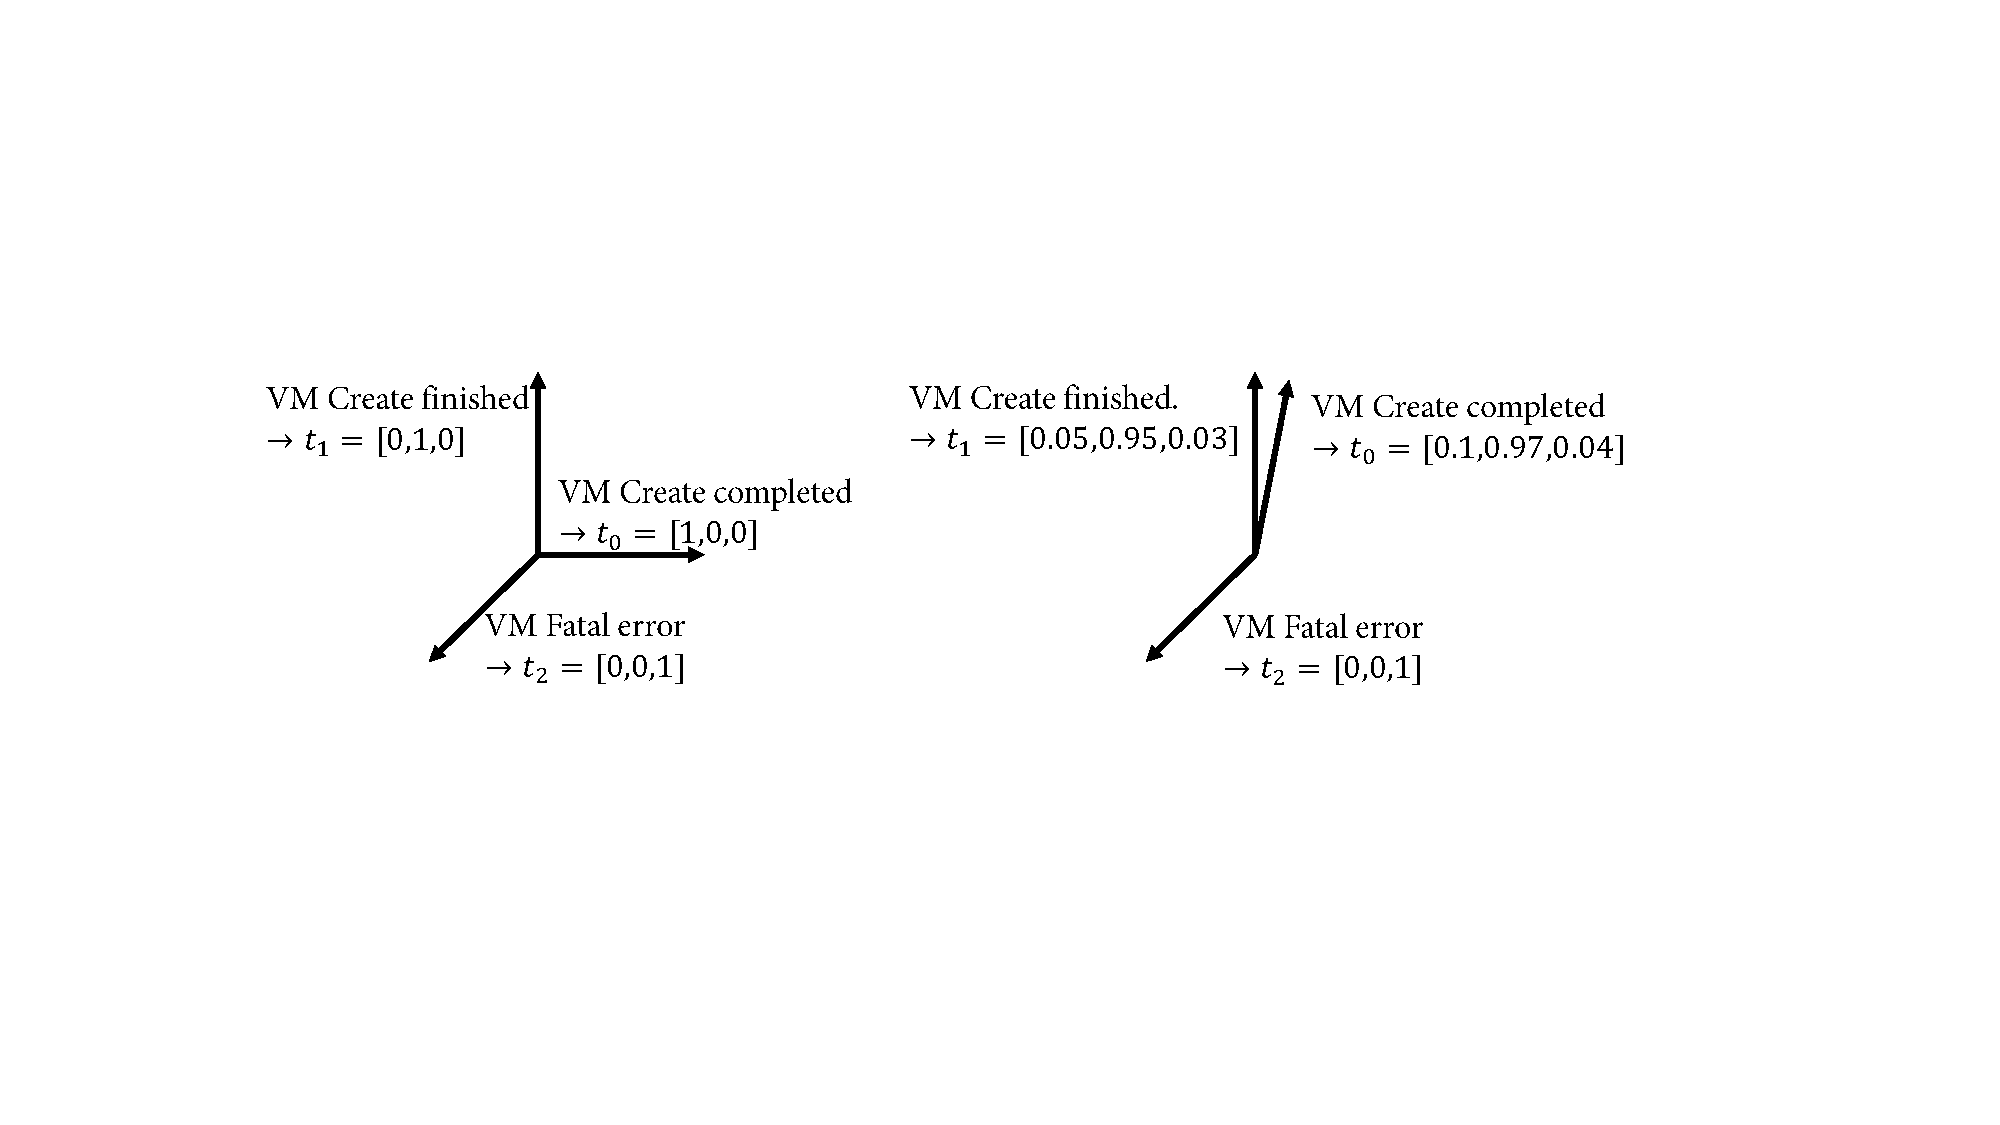
\includegraphics[width=1.0\textwidth]{gfx/chap5/orthogonallogvectors.pdf}}
\caption{Log vectors of three log messages, represented with one-hot encoding (indices, left) and desired representation (right).}
\label{fig:logrepresentations}
\end{figure}

The provision of better log vector representations increases the performances in the anomaly detection tasks. To show the importance of the log representations, we provide an example in Figure~\ref{fig:logrepresentations}. We illustrate three log messages when they are represented with one-hot encoding. The vectors are orthogonal and do not have similarity in-between. Therefore, when a new log message is observed, the model will recognize it as an anomaly, not similar to the learned log messages. This scenario of imperfect representations occurs also when word vectors pretrained on other domain are used. In an ideal case, "VM create finished" and "VM create completed" should be represented closely in the space, while "VM fatal error" should be distant from them. The normal samples should have compact representations, i.e., close distances in the representational space, while anomalies should be distant.

This, in the ultimate case, is shown with the supervised learning scenario of NuLog. When each log message is labeled, the method can identify compositions of words that signal normal and anomaly system states. Furthermore, it utilizes the semantic meaning of the log message to create better log vectors that are robust and produce accurate predictions even on unseen log messages. However, the provision of labeled data from specific systems in production is often prohibitive costly.


\begin{table*}[!t]
% \resizebox{1.0\textwidth}{!}{%
\centering
\begin{tabular}{l|l|c}
\hline
\textbf{Log message (log template $T$ in bold)} & \textbf{Class} & \textbf{Index}  \\ \hline
\textbf{total of} 77 \textbf{ddr error(s) detected and corrected}& normal & $x_0$    \\
\textbf{instruction cache parity error corrected} &normal & $x_1$    \\
\textbf{floating point unavailable interrupt}                             & anomaly       & $x_2$                 \\
\textbf{critical input interrupt (unit=}0x0b \textbf{bit}=0x06\textbf{)} &normal & $x_3$  \\ \hline
\end{tabular}
% }
\caption{Examples of log messages.}
\label{tab:logmessagestemplates}
\end{table*}

Supervised learning can be related to detection of anomalies in the log data by operators. They often analyze the semantic information from the logs and decide whether the message represents a severe system threat or failure. This semantic information is narrow and domain-specific. For example, in Table ~\ref{tab:logmessagestemplates}, $x_2$ and $x_3$ contain similar semantic meanings when observed without domain-specific knowledge. Therefore, both of them would be classified in the same class. However, if observed by a domain-expert knowing that a "floating point" interruption is considerably more severe than an "input" interruption, it would be able to recognize them correctly.

In the following sections of this chapter, we present a method, which addresses these challenges, and bridges the gap in effectiveness from unsupervised to supervised log anomaly detection.


\newpage 

\begin{figure}[!htbp]
\centerline{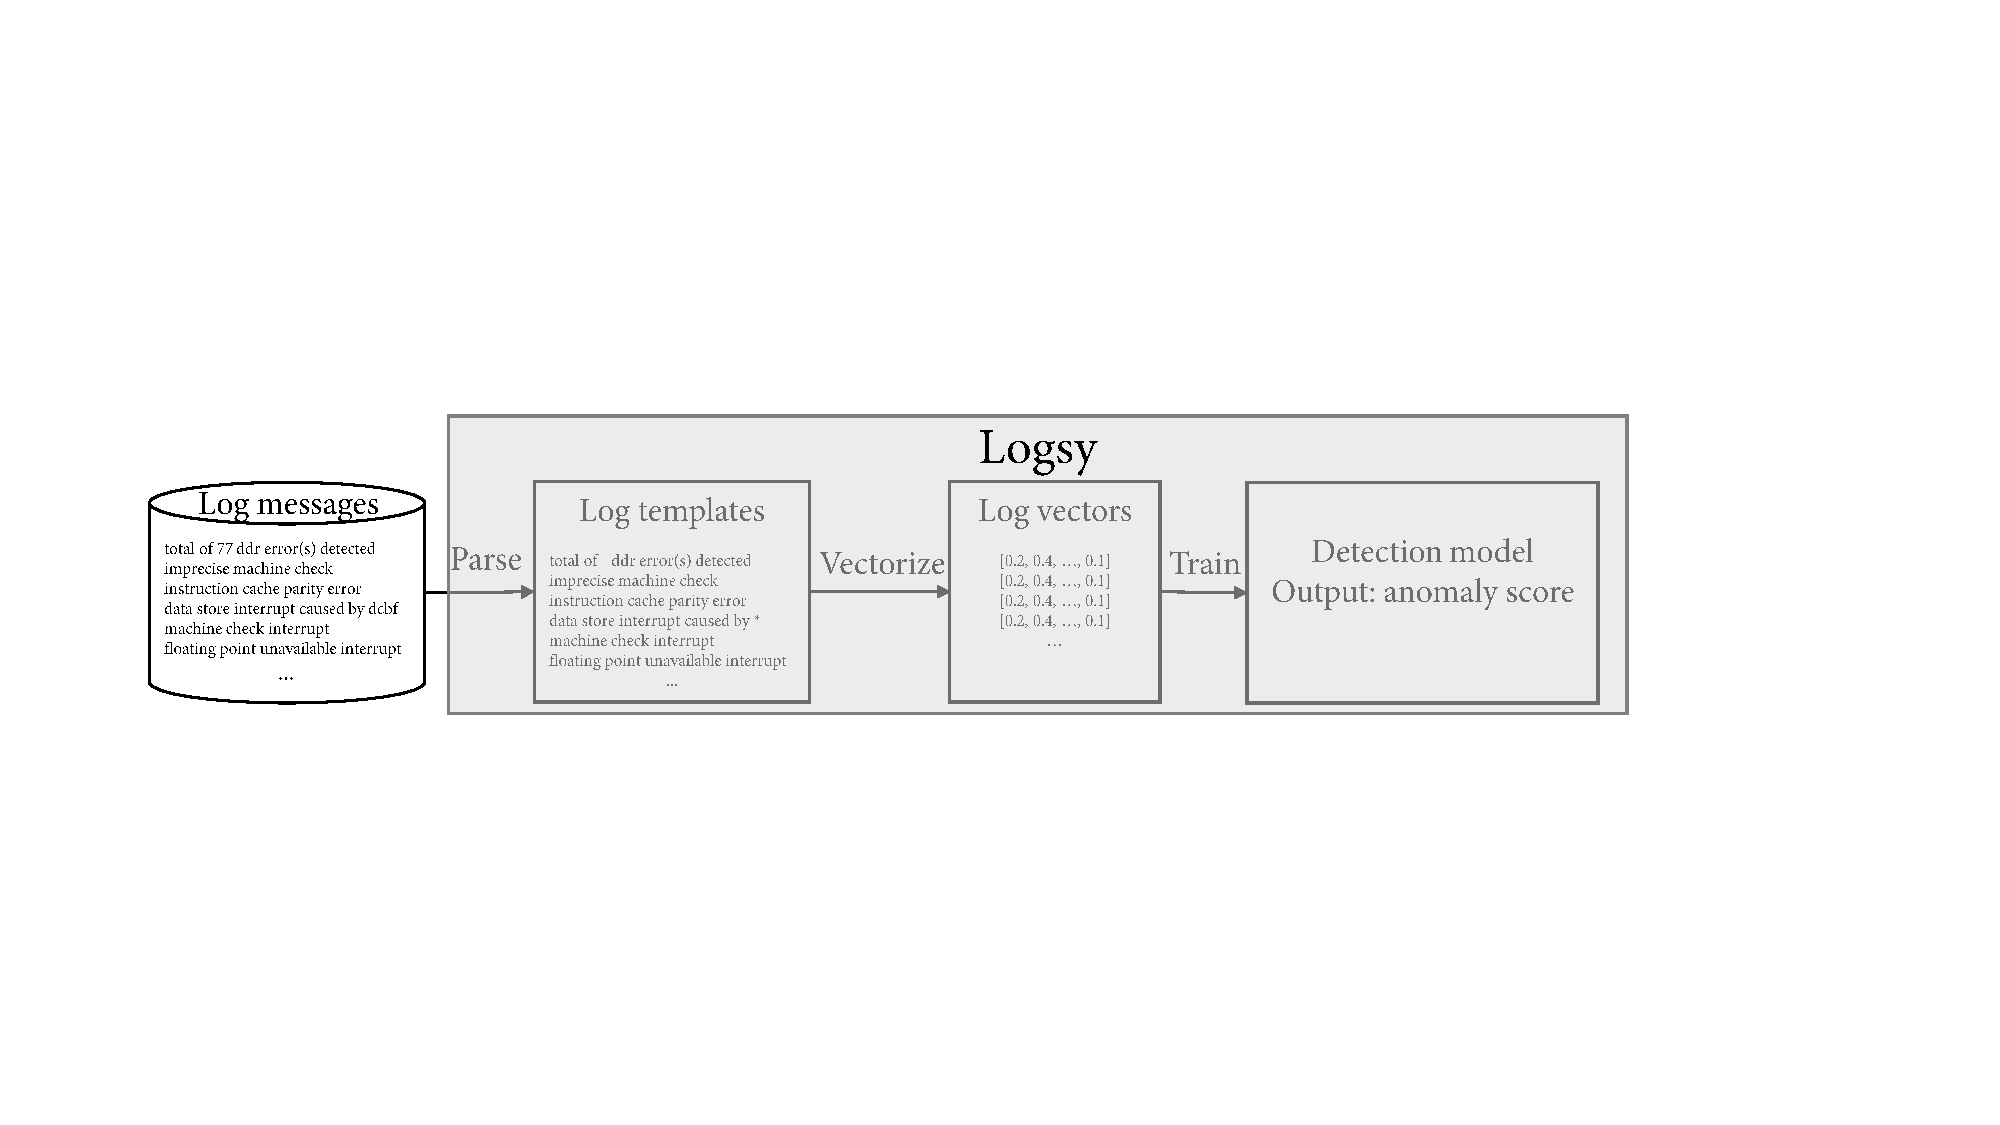
\includegraphics[width=1.0\textwidth]{gfx/chap5/logsypipeline.pdf}}
\caption{Logsy replacing the traditional pipeline of log anomaly detection.}
\label{fig:logsypipeline}
\end{figure}

\section{Log anomaly detection}
The normal log messages ideally should have vector representations with small distances between each other, e.g., concentrated within a tight sphere~\cite{ruff2019deep}. In this section, we present an anomaly detection method denoted as Logsy, which directly addresses the challenge of obtaining compact numerical log vectors. We train a neural network to learn log vectors to separate the normal log data from the system of interest (target system) and log messages from auxiliary log datasets from other systems, easily accessible through the internet. The concept of such a classification approach to anomaly detection is that the auxiliary dataset helps learn a more accurate representation of the normal data while regularizing against over-fitting. This leads to a better generalization for unseen logs. For example, for a target system of interest $T$ where anomaly detection needs to be performed, as auxiliary data, one or more datasets from an open-source log repository could be employed (~\cite{oliner2007supercomputers}). To model the data, we reuse the same transformer architecture as in NuLog. Additionally, we propose a hyperspherical, instead of the traditional hyperplane classification decision boundary, learning objective, to learn compact log vector representations of the normal log messages. This enforces the normal samples to have concentrated (compact) vector representations around the center of a hypersphere. Small distances from the center correspond to normal samples, while large distances correspond to anomalies. The method enables a direct log-to-vector transformation, which can be used to improve the performances of previous related methods.

In this regard, we shift from the traditional log anomaly detection pipeline (Figure~\ref{fig:logsypipeline}). With Logsy, we learn the anomaly score end-to-end from raw log messages. The method does not depend on log parsing and does not utilize a module for obtaining log vectors. The log parsing and log vectorization in Logsy are learned implicitly during the training procedure. 


\subsection{Importance of the auxiliary data}
To elucidate the importance of using the auxiliary data, we relate the anomaly detection task to 
the task of density level set estimation~\cite{tsybakov1997nonparametric}. Steinwart et al.~\cite{steinwart2005classification} stated that this can be interpreted as a binary classification between the normal and anomalous distributions and that the prior on the anomalous distribution is essential for an improved detection. Thus, if we provide information to the model regarding the distribution of the anomalous data, it will increase its performance. For example, we may interpret the class assumption in semi-supervised anomaly detection that a small number of anomaly data points are available and labeled as such prior knowledge or bias~\cite{ruff2019deep}. Moreover, specific types of data can have inherent properties, which enables more informed prior assumptions such as the word representations in texts~\cite{bengio2013representation}, where it is assumed that each word meaning depends on its context.

We assume that drawing realistic samples from some auxiliary easy-access corpus of log data can be considerably more informative for an added description of normal data and anomalies compared to the sampling noise. These samples are replacements for real anomalies used, e.g., in semi-supervised learning approaches.

\section{\textit{Logsy:} Classification-based anomaly detection on logs}
In this section, we explain the proposed method in detail. We describe the data preprocessing, neural network model, log vector representations, and their utilization in the modified objective function for anomaly detection.

To formally define the task, we consider $\mathcal{D}=\{(\mathbf{x_1}, y_1), \dots, (\mathbf{x_n}, y_n)\}$ as training logs from the system of interest where $\mathbf{x_i}$ is a log message whose tokens are represented in $d-dimensional$ space (the log message is represented by $d\times \vert r \vert$ matrix, where $\vert r \vert$ is the maximum number of tokens in all log messages) and $y_i=0; 1 < i \leq n$, assuming that the data in the system of interest are composed mostly of normal samples. $\mathcal{A}=\{(\mathbf{x_n}, y_{n}),\dots, (\mathbf{x_{n+m}}, y_{n+m})\}$, where $m$ is the size of the auxiliary data and $y_i={1}; n < i \leq n+m$. $\phi(\mathbf{x_i}, y_i, \theta): \mathbb{R}^{d \times |r_i|} \rightarrow \mathbb{R}^p \rightarrow [0, a], a \in \mathbb{R}$ is a function represented by a neural network, which maps the input log message token embeddings to vector representations in $\mathbb{R}^p$ (log vectors), and then to an anomaly score. The task is to learn the parameters $\theta$, and then, for each incoming instance in the prediction phase $\mathcal{D}_t=\{(\mathbf{x_1^t}), (\mathbf{x_2^t}),\dots, (\mathbf{x_j^t}), \dots\}$, predict whether it is anomalous or normal based on the anomaly scores, where $t$ indicates the test sample.

\begin{figure}[!b]
\centering
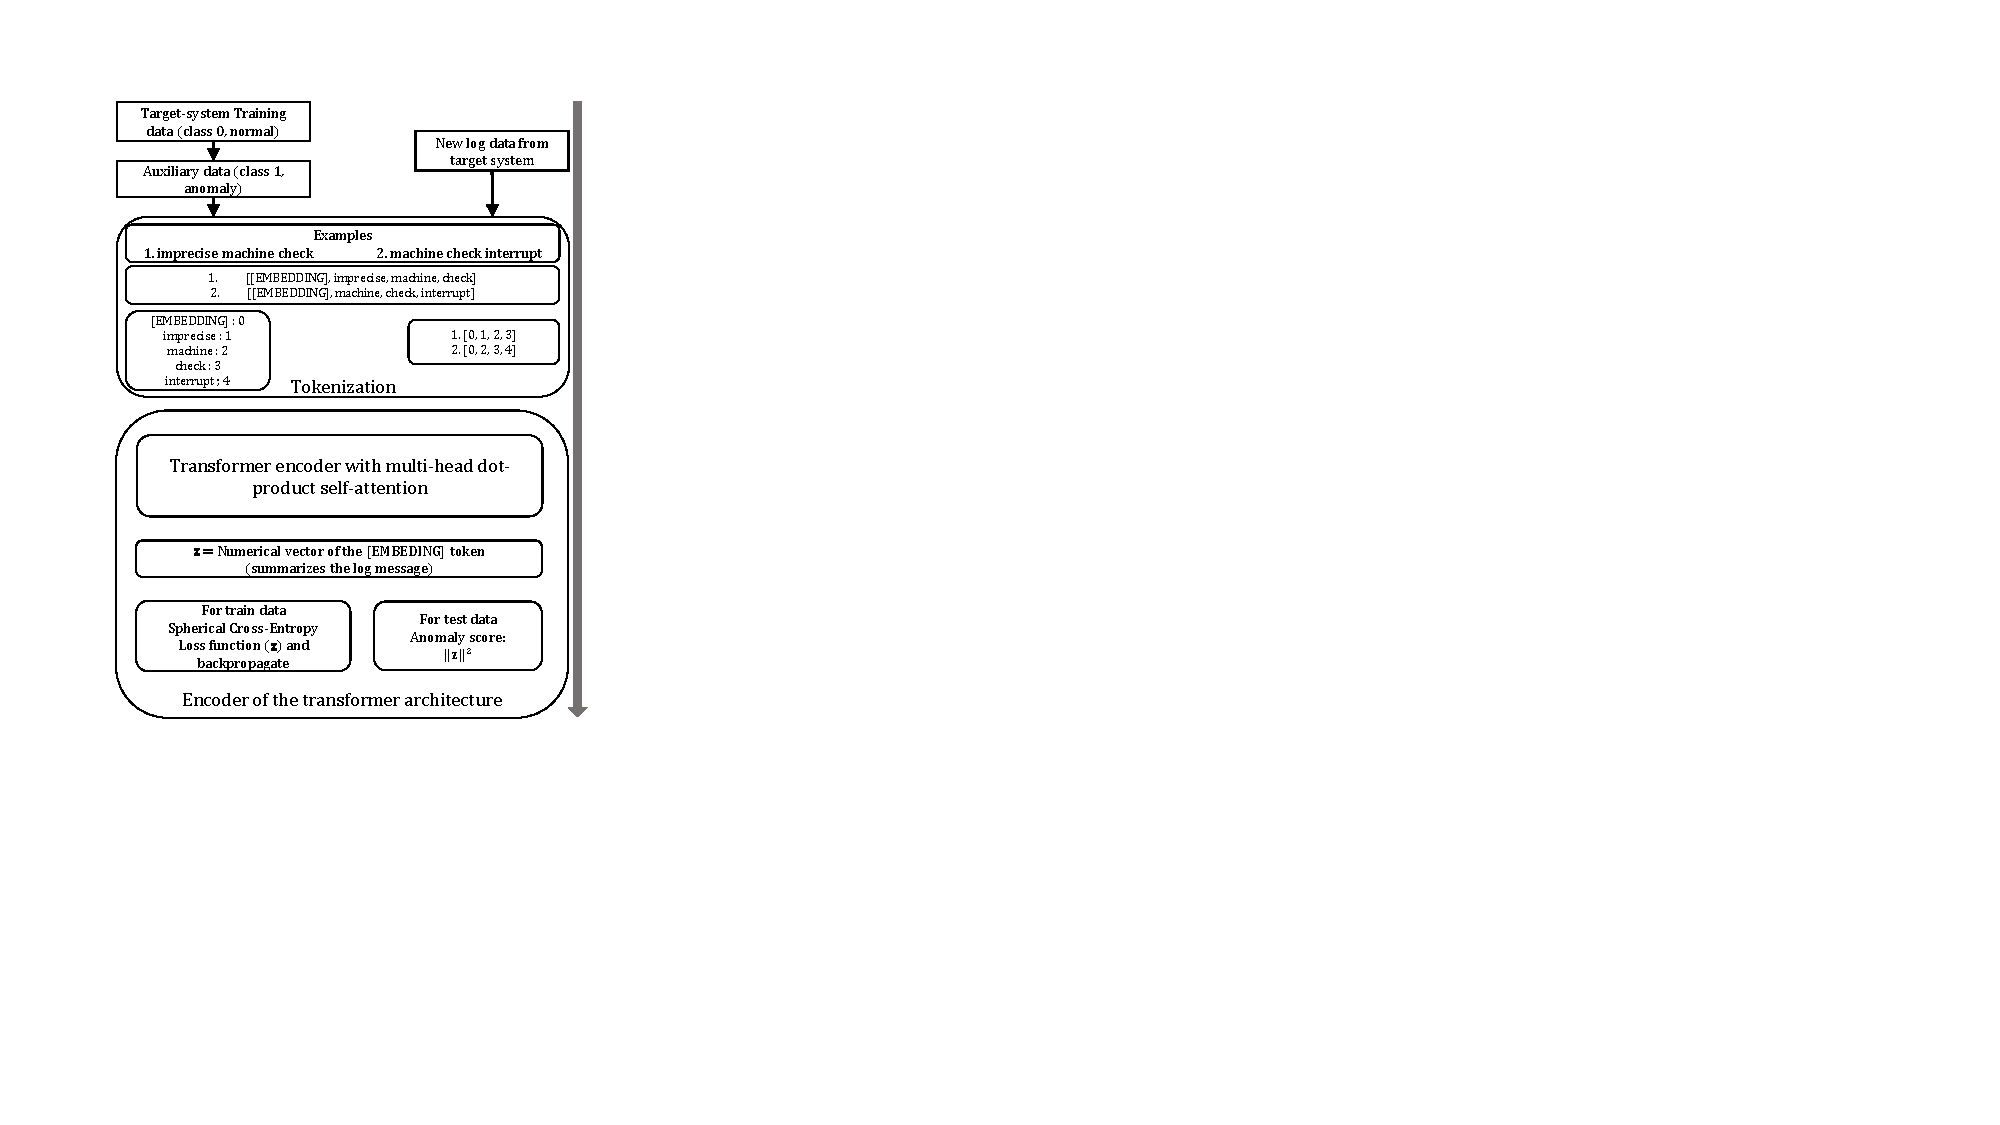
\includegraphics[width=0.8\textwidth]{gfx/chap4/model_loganomalydetection.pdf}
\caption{Overview of the architecture and component details of Logsy.}
\label{overviewmethod}
\end{figure}

\subsection{Logsy}
The method is composed of two main parts, the tokenization of the log messages and neural network model.

\textbf{Tokenization.} The tokenization transforms the raw log messages into a sequence of tokens, as shown in Figure~\ref{overviewmethod}. The same tokenization module as in NuLog is used. In addition, in the tokenization module, we perform cleaning of the log messages. For this purpose, we utilize the standard text preprocessing library NLTK~\cite{loper2002nltk}. The message is initially filtered for HTTP and system path endpoints (e.g., /p/gb2/stella/RAPTOR/). Every capital letter is converted to the lowercase letter. All ASCII special characters are removed. The log message is split into word tokens. We remove every token that contains numerical characters, as they often represent variables in the log message and are not informative. Additionally, we remove the most commonly used English words that are in the stop word dictionary of NLTK (e.g., the and is). Similar to the case of NuLog, to the front of the tokenized log message, a special \texttt{EMBEDDING} token is added. In the model, the \texttt{EMBEDDING} token attends over all original tokens from the sample, which enables the model to summarize the context of the log message in the vector representation. All tokens from every log message form a dictionary $\mathbb{V}$ with a size of $|\mathbb{V}|$, where each word is represented with an integer label $i \in {0, 1, \dots,|\mathbb{V}|-1}$. An advantage of Logsy over previous log anomaly detection approaches is that it does not depend on log parsers as a preprocessing step (only cleaning). We consider the tokenized log message as a direct input to the model. As an advantage, no loss of information from the log message exists, owing to the imperfections in the log parsing methods.

\textbf{Model}. Logsy has two operation modes, offline and online. During the offline phase, log messages are used to tune all model parameters through back-propagation and optimal hyperparameters are selected. During the online phase, every log message is passed forward through the saved model. This generates the respective log vector representation $\mathbf{z}$ and anomaly score for each message.

The core model architecture is the Transformer encoder, similar to NuLog. As a detailed description of the transformer encoder was already presented in~\autoref{NuLog}, we describe only the major parts.
The model applies two operations on the input tokens, token vectorization (word embeddings) and positional encoding. The subsequent structure is the encoder of the transformer~\cite{vaswani2017attention} module with a multi-head self-attention, which uses the result of these operations as an input. 
At the output of the encoder, the transformed vector representation from the initial tokens exists. The \texttt{EMBEDDING} token has its transformed representation $\mathbf{z}$, which is used as a final log vector representation.
The final element of the model consists of a single linear layer. It receives the vector $\mathbf{z}$ from the \texttt{EMBEDDING} token and uses it for optimizing the model. Based on the loss function, gradients are back-propagated to tune the parameters of the model. 

\subsection{Objective function}
To ensure learning of the intrinsic differences between normal and anomaly log samples, we propose a spherical loss function. It is designed to integrate the previously mentioned assumption that normal data are often concentrated, with small distances between the normal samples, while also learning properties to distinct from anomalous samples. This is carried out by employing a radial classification loss, which enforces a compact hyperspherical decision region for the normal samples.

To derive the loss, we start with the standard binary cross entropy. $\mathcal{D}=\{(\mathbf{x_1}, y_1), \dots, (\mathbf{x_{n+m}}, y_{n+m})\}$ is the concatenation of the training logs from the system of interest and auxiliary data with $\mathbf{x_i} \in \mathbb{R}^{d\times|r_i|}$, where $|r_i|$ is the number of tokens in the log message and each token is a vector represented in $d-dimensional$ space. $y_i \in \{0,1\}$; $y_i=0$ denotes normal samples (target system), while $y_i=1$ denotes an anomaly (auxiliary data). $\phi(\mathbf{x_i}, \theta): \mathbb{R}^d \rightarrow \mathbb{R}^p$ is our encoder architecture, which maps the $|x_i|$ word embeddings form the log message to a $p-dimensional$ vector. $l:\mathbb{R}^p \rightarrow [0,1]$ is a function that maps the output to an anomaly score. Using $\phi(\mathbf{x_i}, \theta)$ and $l(\cdot)$, the standard binary cross-entropy loss can be expressed by

\begin{equation}
    - \frac{1}{n}\sum_{i=1}^{n}(1-y_i)\log l(\phi(\mathbf{x_i}; \theta)) + y_i\log (1-l(\phi(\mathbf{x_i}; \theta))).
\end{equation}\label{bce}

For the standard classifier function, the $p-dimensional$ representation is transformed through a linear layer followed by the sigmoid activation function,

\begin{equation}\begin{aligned}
    - \frac{1}{n}\sum_{i=1}^{n}(1-y_i)\log((1+\exp(-\mathbf{w}^T \phi(\mathbf{x_i}, \theta)))^{-1}) \\
    +  y_i\log(1-(1+\exp(-\mathbf{w}^T \phi(\mathbf{x_i}, \theta)))^{-1})\end{aligned}.
\end{equation}\label{bcesigmoid}

In the standard binary classifier with the sigmoid function, the decision boundary is half-space, as depicted in gray in Figure~\ref{hyperplane}. The representation of the log messages is not guaranteed to be compact in this case. It is very likely that the normal samples are scattered throughout the space with varying potentially very large distances between them. To enforce compactness of the representations of the log messages, we utilize the Gaussian radial basis function, $l(\cdot)$,

\begin{equation}
    l(\mathbf{z})= \exp(-\Vert \mathbf{z} \Vert ^2).
\end{equation}

By replacing the function into the loss function, we obtain the hyperspherical classifier,
\begin{equation}\begin{aligned}
    - \frac{1}{n}\sum_{i=1}^{n}(1-y_i)\log(\exp(-\Vert \phi(\mathbf{x_i}; \theta) \Vert ^2)) \\
    +  y_i\log(1-\exp(-\Vert \phi(\mathbf{x_i}; \theta) \Vert ^2)) \\
    =  \frac{1}{n}\sum_{i=1}^{n}(1-y_i)\Vert \phi(\mathbf{x_i}; \theta) \Vert ^2 \\
    -  y_i\log(1-\exp(-\Vert \phi(\mathbf{x_i}; \theta) \Vert ^2)).\end{aligned}
\label{hce}
\end{equation}.


This ensures compactness of the normal samples, which are enforced to be around the center of a sphere $\mathbf{c}=\mathbf{0}$. For normal samples, i.e., $y_i=0$, the loss function minimizes the distance to $\mathbf{c}$. This leads to low values for the left term in Equation~\ref{hce}. In contrast, the right term of the loss function favors large distances for the anomalous samples. As shown in Figure~\ref{hypersphere}, the radial basis function has a spherical (circle in 2D) decision boundary, located between the gray and black areas. The center of the sphere $c$ could be any constant value, which is not relevant during the optimization.


\begin{figure}[!t]
\minipage{0.35\columnwidth}
  
\includegraphics[width=\linewidth]{gfx/chap4/hyperplane.pdf}
  \caption{Hyperplane classifier with sigmoid.}\label{hyperplane}
\endminipage\hfill
\minipage{0.45\columnwidth}
  
\includegraphics[width=\linewidth]{gfx/chap4/hypersphere.pdf}
  \caption{Hypersphere classifier using the radial function instead of sigmoid.}\label{hypersphere}
\endminipage

\end{figure}

However, for such spherical classifiers~\cite{ruff2019deep}, the model may be prone to learn trivial solutions by mapping the inputs to output a constant vector, $c$. However, the proposed loss function will not find the trivial solution because of the second term in the equation, which represents the auxiliary data or anomalies. To formally demonstrate this statement, we consider $\phi(\cdot)$ as an encoder network, which maps every log message to $\mathbf{c}$ (trivial solution). Thus, $\phi(\cdot)=\mathbf{0}$. In this case, the second term in Equation~\ref{hce} for $y_i=1$ will be infinity or very large value, which acts as a regularizer and prevents learning $\mathbf{c}$ as a trivial vector representation,

\begin{equation}\begin{aligned}
    -\log(1-\exp(-\Vert \mathbf{0} \Vert ^2))= -log(\mathbf{0}).
    \end{aligned}
\end{equation}\label{hcedecomposed}

\subsection{Anomaly score and detection of anomalies}
Considering that the assumption of the objective function enforces compact, close to the center of the sphere $\mathbf{c}=\mathbf{0}$, representations, we define our anomaly score as the distance of the log vectors (obtained from the \texttt{EMBEDDING} token) to the center $\textbf{c}$ of the hypersphere,

\begin{equation}
    A(\mathbf{x_i}) = \Vert \phi(\mathbf{x_i}; \theta) \Vert ^2.
\end{equation}

We attribute low anomaly scores $A(\mathbf{x_i})$ to normal log messages, while large scores to anomalies. To decide whether the sample is anomalous or normal, we use a threshold $\mathcal{E}$. If the anomaly score $A(\mathbf{x_i}) > \mathcal{E}$, the sample is an anomaly; otherwise, we consider it as normal. This concludes the explanation of the method. We describe two properties of the model below.


\subsection{Learning with an additional expert input}
Most computer systems are, to some extent, supervised and operated by an administrator. Over time, the administrator can manually inspect a small portion of the events and provide labels.
As an additional option, Logsy allows incorporation of such labels from the target system. The second term in Equation~\ref{hce}, used for the auxiliary data, could be also utilized for the inclusion of operator-labeled samples. This enables the addition of even more realistic, but costly anomaly samples, which help learn the anomaly distribution and improve the performance. The labeled samples can be added together with the auxiliary data and the model needs to be retrained or the following procedure should be utilized:
\begin{enumerate}
    \item Train the model with the auxiliary data.
    \item Replace the auxiliary data with the labeled samples.
    \item Continue the training of the model only with the labeled sample until convergence.
\end{enumerate}

The replacement of the auxiliary data with the labeled samples allows the model to only fine-tune its parameters in a few epochs. This preserves the already learned information from the larger auxiliary dataset as a bias to the fine-tuning procedure. In the experiments, we show that the inclusion of a small portion of labeled samples improves the performance of the model.



\begin{figure}[!b]
\centering
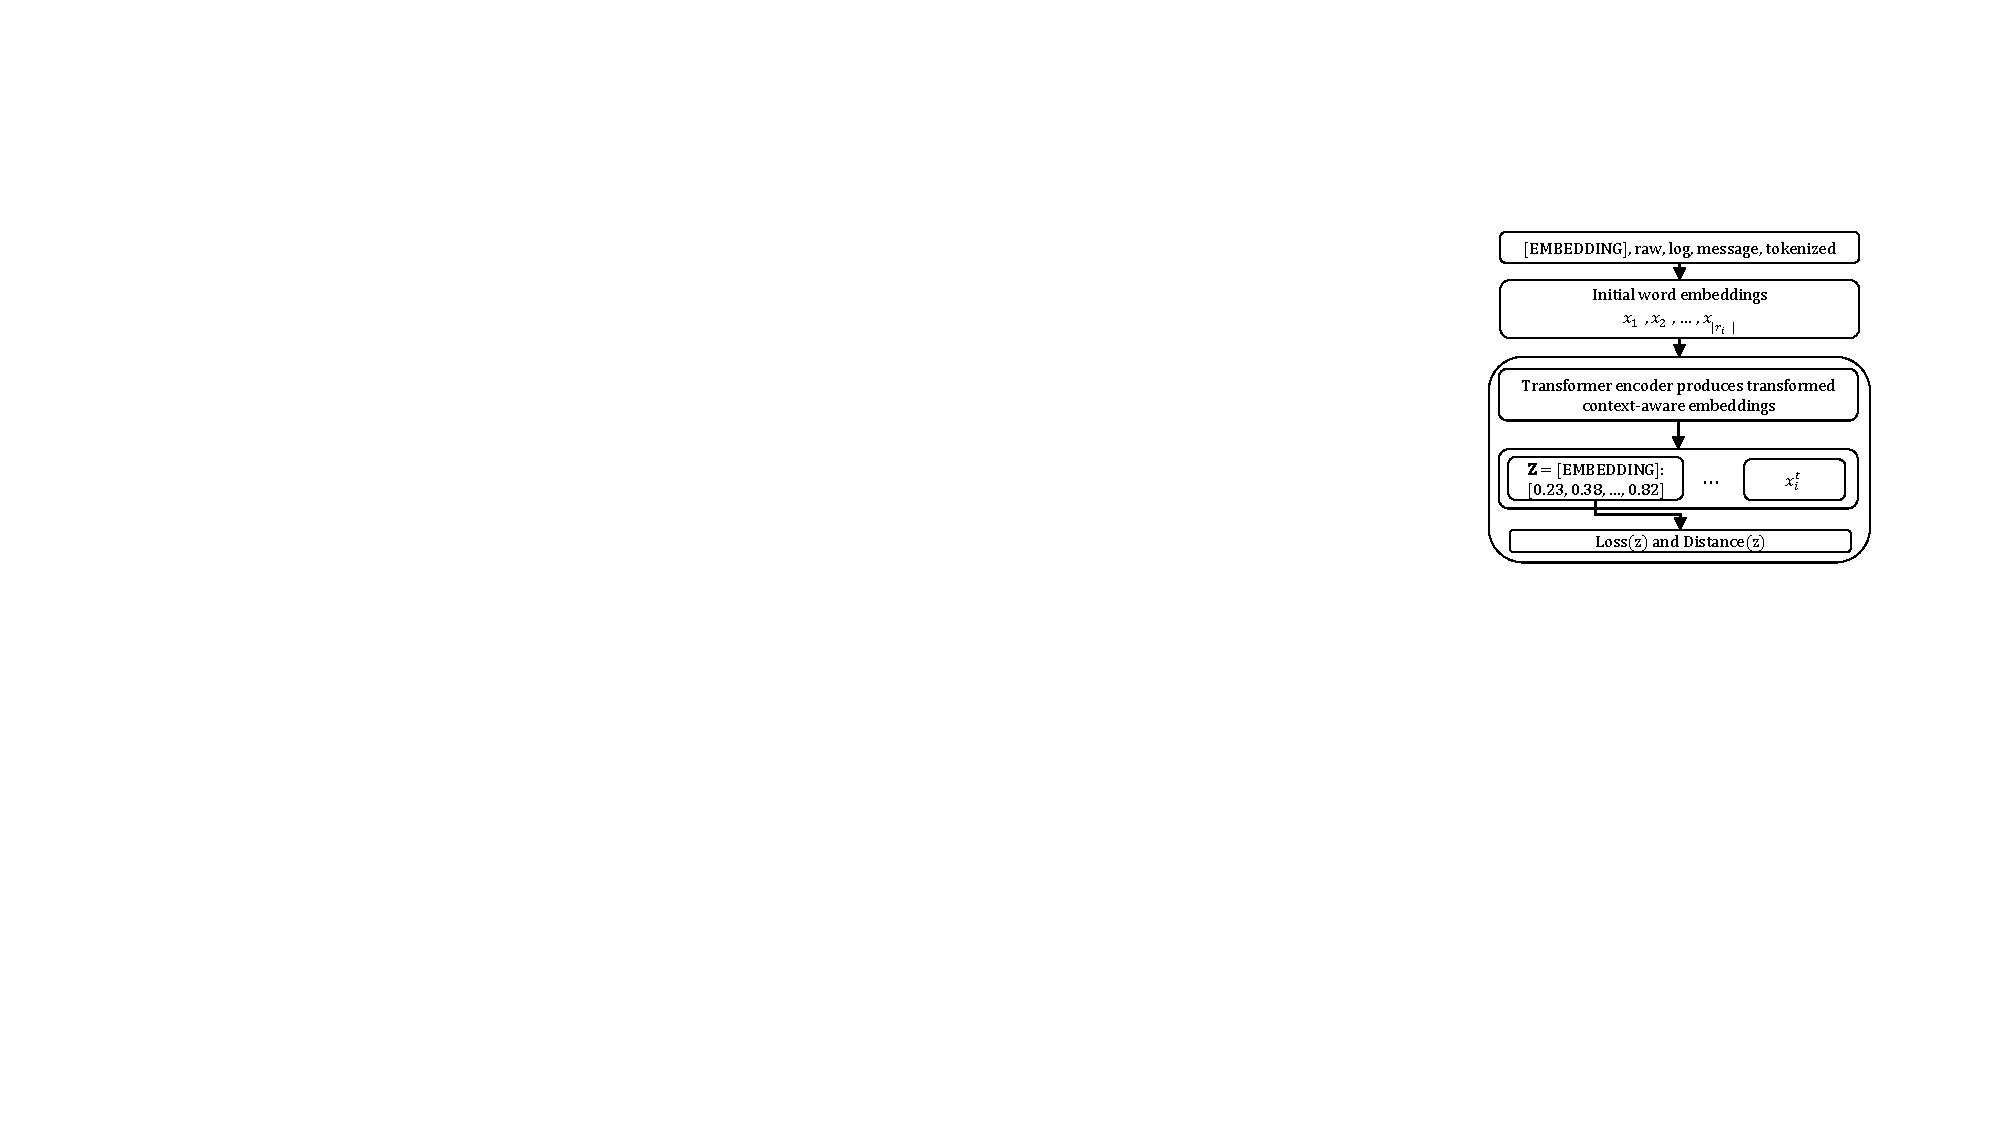
\includegraphics[width=0.7\textwidth]{gfx/chap5/gettingembeddings.pdf}
\caption{Provision of the log vector embedding using the special 'EMBEDDING' token that summarizes the context of the log message.}
\label{fig:gettingembeddings}
\end{figure}


\begin{figure}[!t]
    \centering
    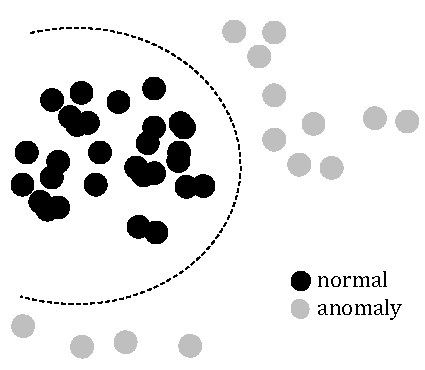
\includegraphics[width=0.6\columnwidth]{gfx/chap4/embeddingsinspace.pdf}
    \caption{Ideal distribution of the log vector representations in space.}
    \label{fig:lowdimensions}
\end{figure}


\subsection{Vector representations of the logs}\label{vectorrepresentations}
Logsy can also be utilized to obtain numerical log representations as they are used in the traditional log anomaly detection pipeline. These representations, as described above, are used by the objective function and to obtain anomaly score in Logsy, but could be also used to replace other less powerful representations, e.g., term-frequency inverse document frequency (TF-IDF) in previous log-based anomaly detection methods such as the PCA ~\cite{xu2009detecting}), to enhance their anomaly detection. 

In Figure~\ref{fig:gettingembeddings}, we illustrate the process of obtaining the log embeddings. The transformer encoder transforms each of the vectors of the input tokens $x_1, x_2, \dots, x_{|r_i|}$ to an abstract representation $x_1^t, x_2^t, \dots, x_{|r_i|}^t$. As only the vector of the first \texttt{EMBEDDING} token is used for optimizing the loss function, it summarizes the context of the log message. In Figure~\ref{fig:lowdimensions}, we illustrate a lower-dimensional plot of the ideal log representations. A decision boundary (dashed line) can be drawn to optimally separate the classes. We demonstrate such behavior in the evaluation section on real data with Logsy, where we show the normal and abnormal sample distributions in a low-dimensional space.

\newpage

\section{Evaluation}
We perform various experiments to quantify the performance of Logsy. We compare the method against two publicly available baselines, DeepLog and PCA, on three real-world HPC log datasets. We describe the main properties of the datasets and experimental setup and present the results. We empirically and qualitatively evaluate the log vector representations from Logsy. We utilized them in the PCA method, which provided an improved performance.



\begin{table*}[!b]
\resizebox{\columnwidth}{!}{%
\begin{tabular}{c|c|c|c|c|c|c|c}
\hline
\textbf{System} & \textbf{Vendor} & \textbf{\#Processors} & \textbf{Days} & \textbf{\#Messages} & \textbf{Data Size (GB)} & \textbf{\#Anomalies} & \textbf{\#Anomalies (5m)} \\ \hline
Blue Gene/L     & IBM             & 131072                & 215           & 4747963             & 1207                    & 348460               & 348460                 \\
Thunderbird     & Dell            & 9024                  & 244           & 211212192           & 27367                   & 3248239              & 226287                 \\
Spirit          & HP              & 1028                  & 558           & 272298969           & 30289                   & 172816564            & 764890 \\\hline               
\end{tabular}
}
\caption{Target datasets.}
    \label{datasets}
\end{table*}




\subsection{Experimental setup}
We select three open real-world datasets from HPC systems for the evaluation as target systems, Blue Gene/L (BGL), Spirit, and Thunderbird~\cite{oliner2007supercomputers}. Table~\ref{datasets} summarizes the main characteristics of the datasets. They share an important characteristic associated with the appearance of numerous new log messages in the timeline of the data, i.e., the systems change over time. Furthermore, as an additional dataset for enriching the auxiliary data in all experiments, we use the HPC RAS log dataset~\cite{zheng2011co}. Owing to the absence of labels, this dataset cannot be used for evaluation purposes; it cannot be a target dataset. 

For each target dataset, as auxiliary data to represent the anomaly class, we use logs from the remaining datasets. Notably, the target vs. auxiliary splits ensure that no leak of information from the target system into the auxiliary data exists. The auxiliary logs consist only of easily accessible logs from other systems through the internet. 
The nonanomalous samples from the target system are the target dataset. For example, when Blue Gene/L is our system of interest (i.e., the target system), percentages of the negative samples of Thunderbird, Spirit, and RAS are used as an auxiliary dataset to represent the anomaly class. These auxiliary samples could be also error messages obtained from online code repositories (e.g., GitHub).
We perform anomaly detection on the test samples from the target dataset to determine the scores. The setup is illustrated in Figure~\ref{fig:datasplits}.


\begin{figure}[!htbp]
    \centering
    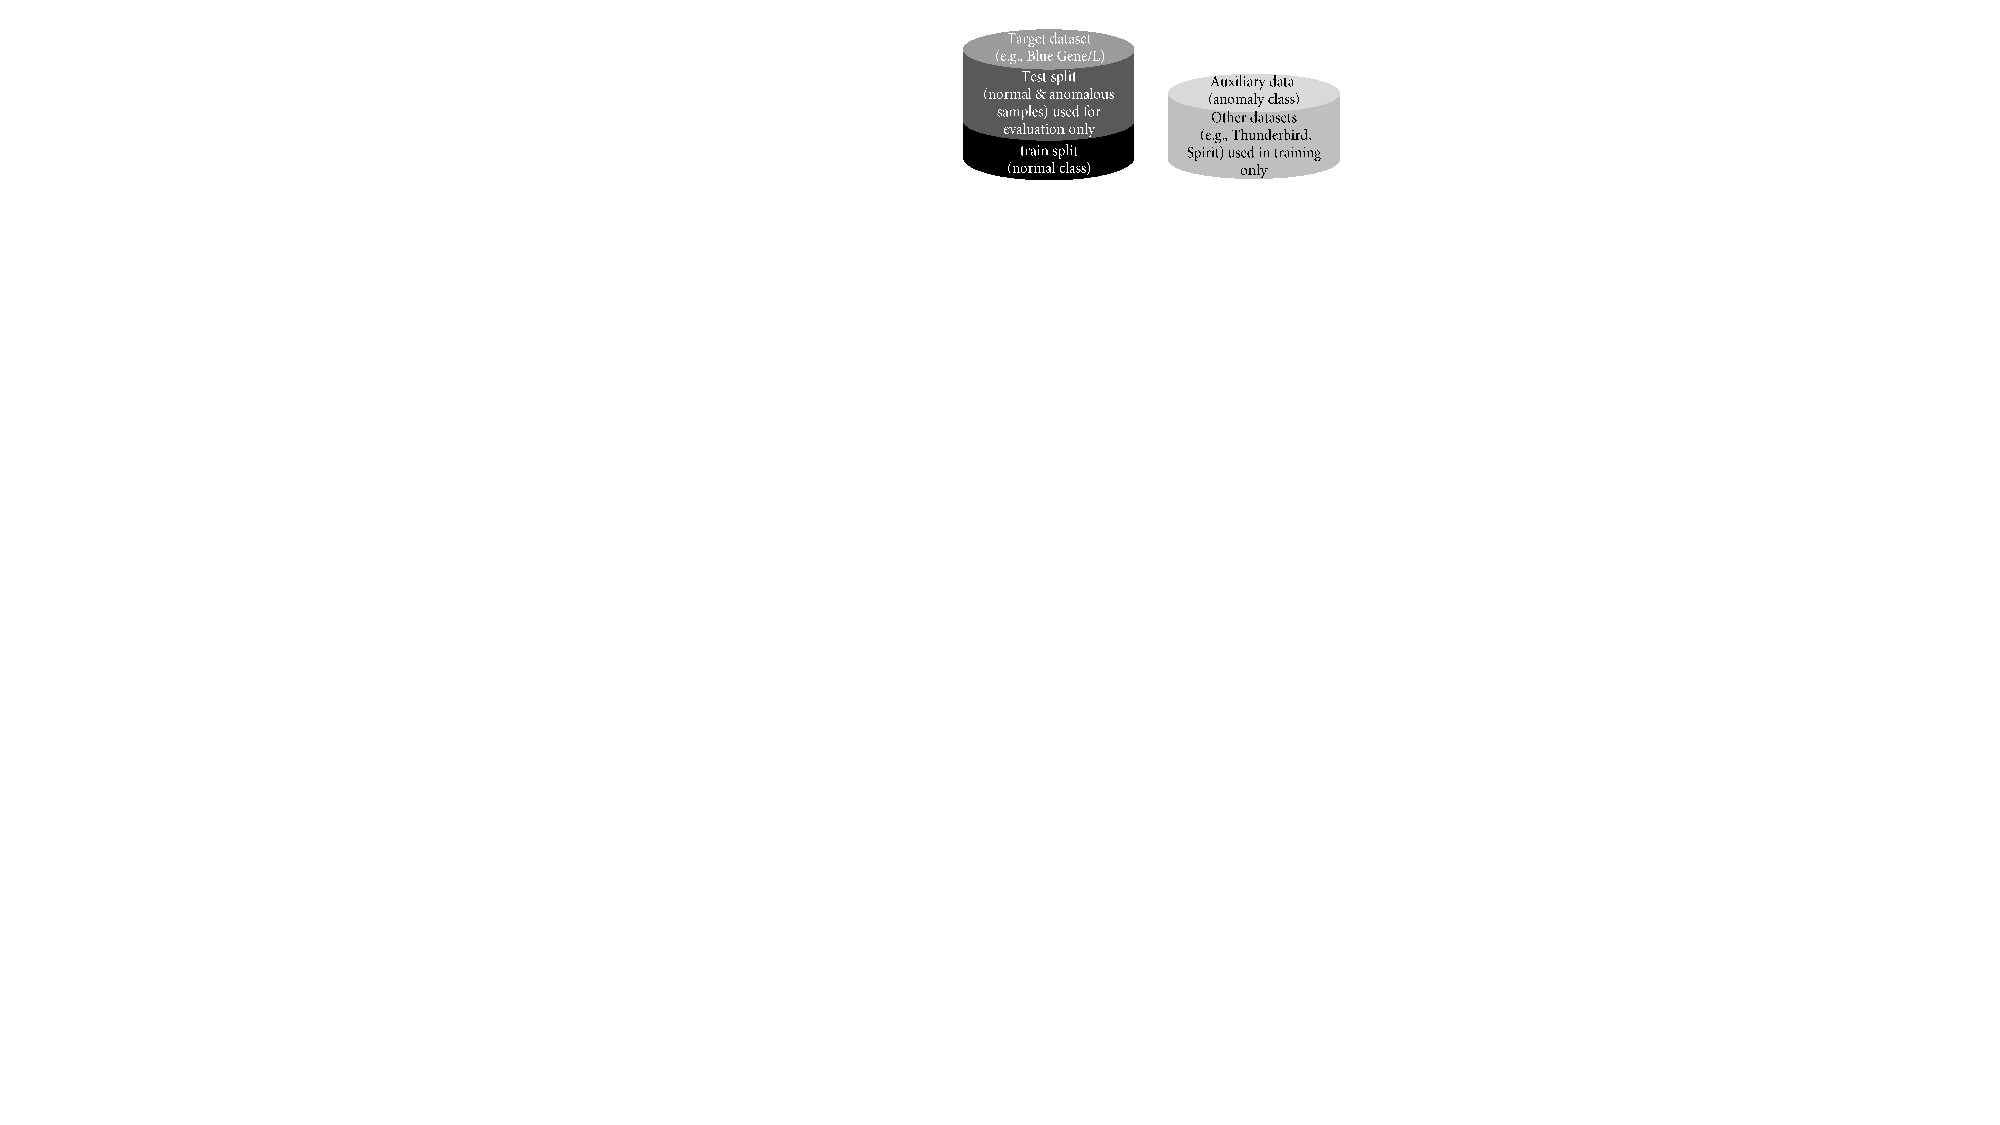
\includegraphics[width=0.7\columnwidth]{gfx/chap5/datasplits.pdf}
    \caption{Illustration of the target and auxiliary data split.}
    \label{fig:datasplits}
\end{figure}

Table~\ref{datasets} shows that Thunderbird and Spirit are quite large datasets of more than 200 million log messages. For a computation time reduction, we restrict the data size on the first 5 million log messages, sorted by timestamp. We ensure that the 5 million log lines preserve the properties of the dataset. Table~\ref{unqiuemessages} shows the number of unseen logs in the test data split. The Blue Gene/L dataset has less than 5 million messages; thus, we keep all of them. \#Anomalies (5m) shows the number of anomalous log messages in the 5 million messages. 



To evaluate the robustness and generalization of Logsy in detail, we carry out several experiments with different train--test splits on the target dataset. To ensure that the test data contain new log messages previously unseen in the training, we always split the data sorted by the timestamp of the log messages. We perform five different data splits to cover as many scenarios as possible: 10\% training -- 90\% test data, 20\% training -- 80\% test, 40\% training -- 60\% test, 60\% training -- 40\% test, and 80\% training -- 20\% test.

The number of unique log messages after the tokenization is presented in Table~\ref{unqiuemessages}. Every split contains unseen log messages in the test data, which do not exist in the train split. The evaluation of the method on such splits demonstrates the model generalization. The decrease in the size of the training data increases the number of novel log messages in the test split.

\begin{table}[!htbp]
\centering
\begin{tabular}{c|c|c|c|c|c|c}
\hline
{\textbf{System}} & \multicolumn{5}{c|}{\textbf{\begin{tabular}[c]{@{}c@{}}\#Unique log messages in \\ test and not present in train for every split\end{tabular}}} & {\textbf{\begin{tabular}[c]{@{}c@{}}\#Total unique\\ messages\end{tabular}}} \\ \cline{2-6}
                                 & \multicolumn{1}{l|}{10\%}     & \multicolumn{1}{l|}{20\%}     & \multicolumn{1}{l|}{40\%}     & \multicolumn{1}{l|}{60\%}     & 80\%    &                                                                                             \\ \hline
Blue Gene/L                      & 2679                          & 2621                          & 2256                          & 2231                          & 465     & 4486                                                                                        \\
Thunderbird                      & 334                           & 127                           & 71                            & 27                            & 12      & 3279                                                                                        \\
Spirit                           & 1091                          & 1028                          & 297                           & 129                           & 73      & 3441                                                                                        \\ \hline
\end{tabular}
\caption{Number of new log messages in the test in every train/test split.}
\label{unqiuemessages}
\end{table}

\subsection{Baselines}
We compare Logsy against two publicly available baseline methods, PCA~\cite{xu2009detecting} and Deeplog~\cite{du2017deeplog}. Industry related studies showed that LogAnomaly~\cite{meng2019loganomaly} has a state-of-the-art performance. However, it has no publicly available implementation. LogAnomaly provides an improvement compared to DeepLog with an F1 score of 0.03. The results of both methods are comparable. The parameters of these methods are tuned to produce their best F1 scores.

\subsection{Implementation details}
Every log message during the tokenization is truncated to a maximum of $\max(\vert r_i \vert)=50$ tokens. Logsy has two layers of the transformer encoder. The words are embedded with 16 neural units. The higher-level vector representations obtained with the transformer encoding have the same sizes. The size of the feed-forward network that uses the output of the multi-head self-attention mechanism is also 16, which provides the '[EMBEDDING]' vector with the same size. For the optimization procedure for every experiment, we use a dropout of 0.05, Adam optimizer with a learning rate of 0.0001, and weight decay of 0.001. We address the imbalanced number of normal versus anomaly samples by adding weights to the loss function for the two classes, 0.5 for the normal and 1.0 for the anomaly class. The models are trained until convergence and later evaluated on the respective test split.




\begin{figure*}[!t]
    \centering
    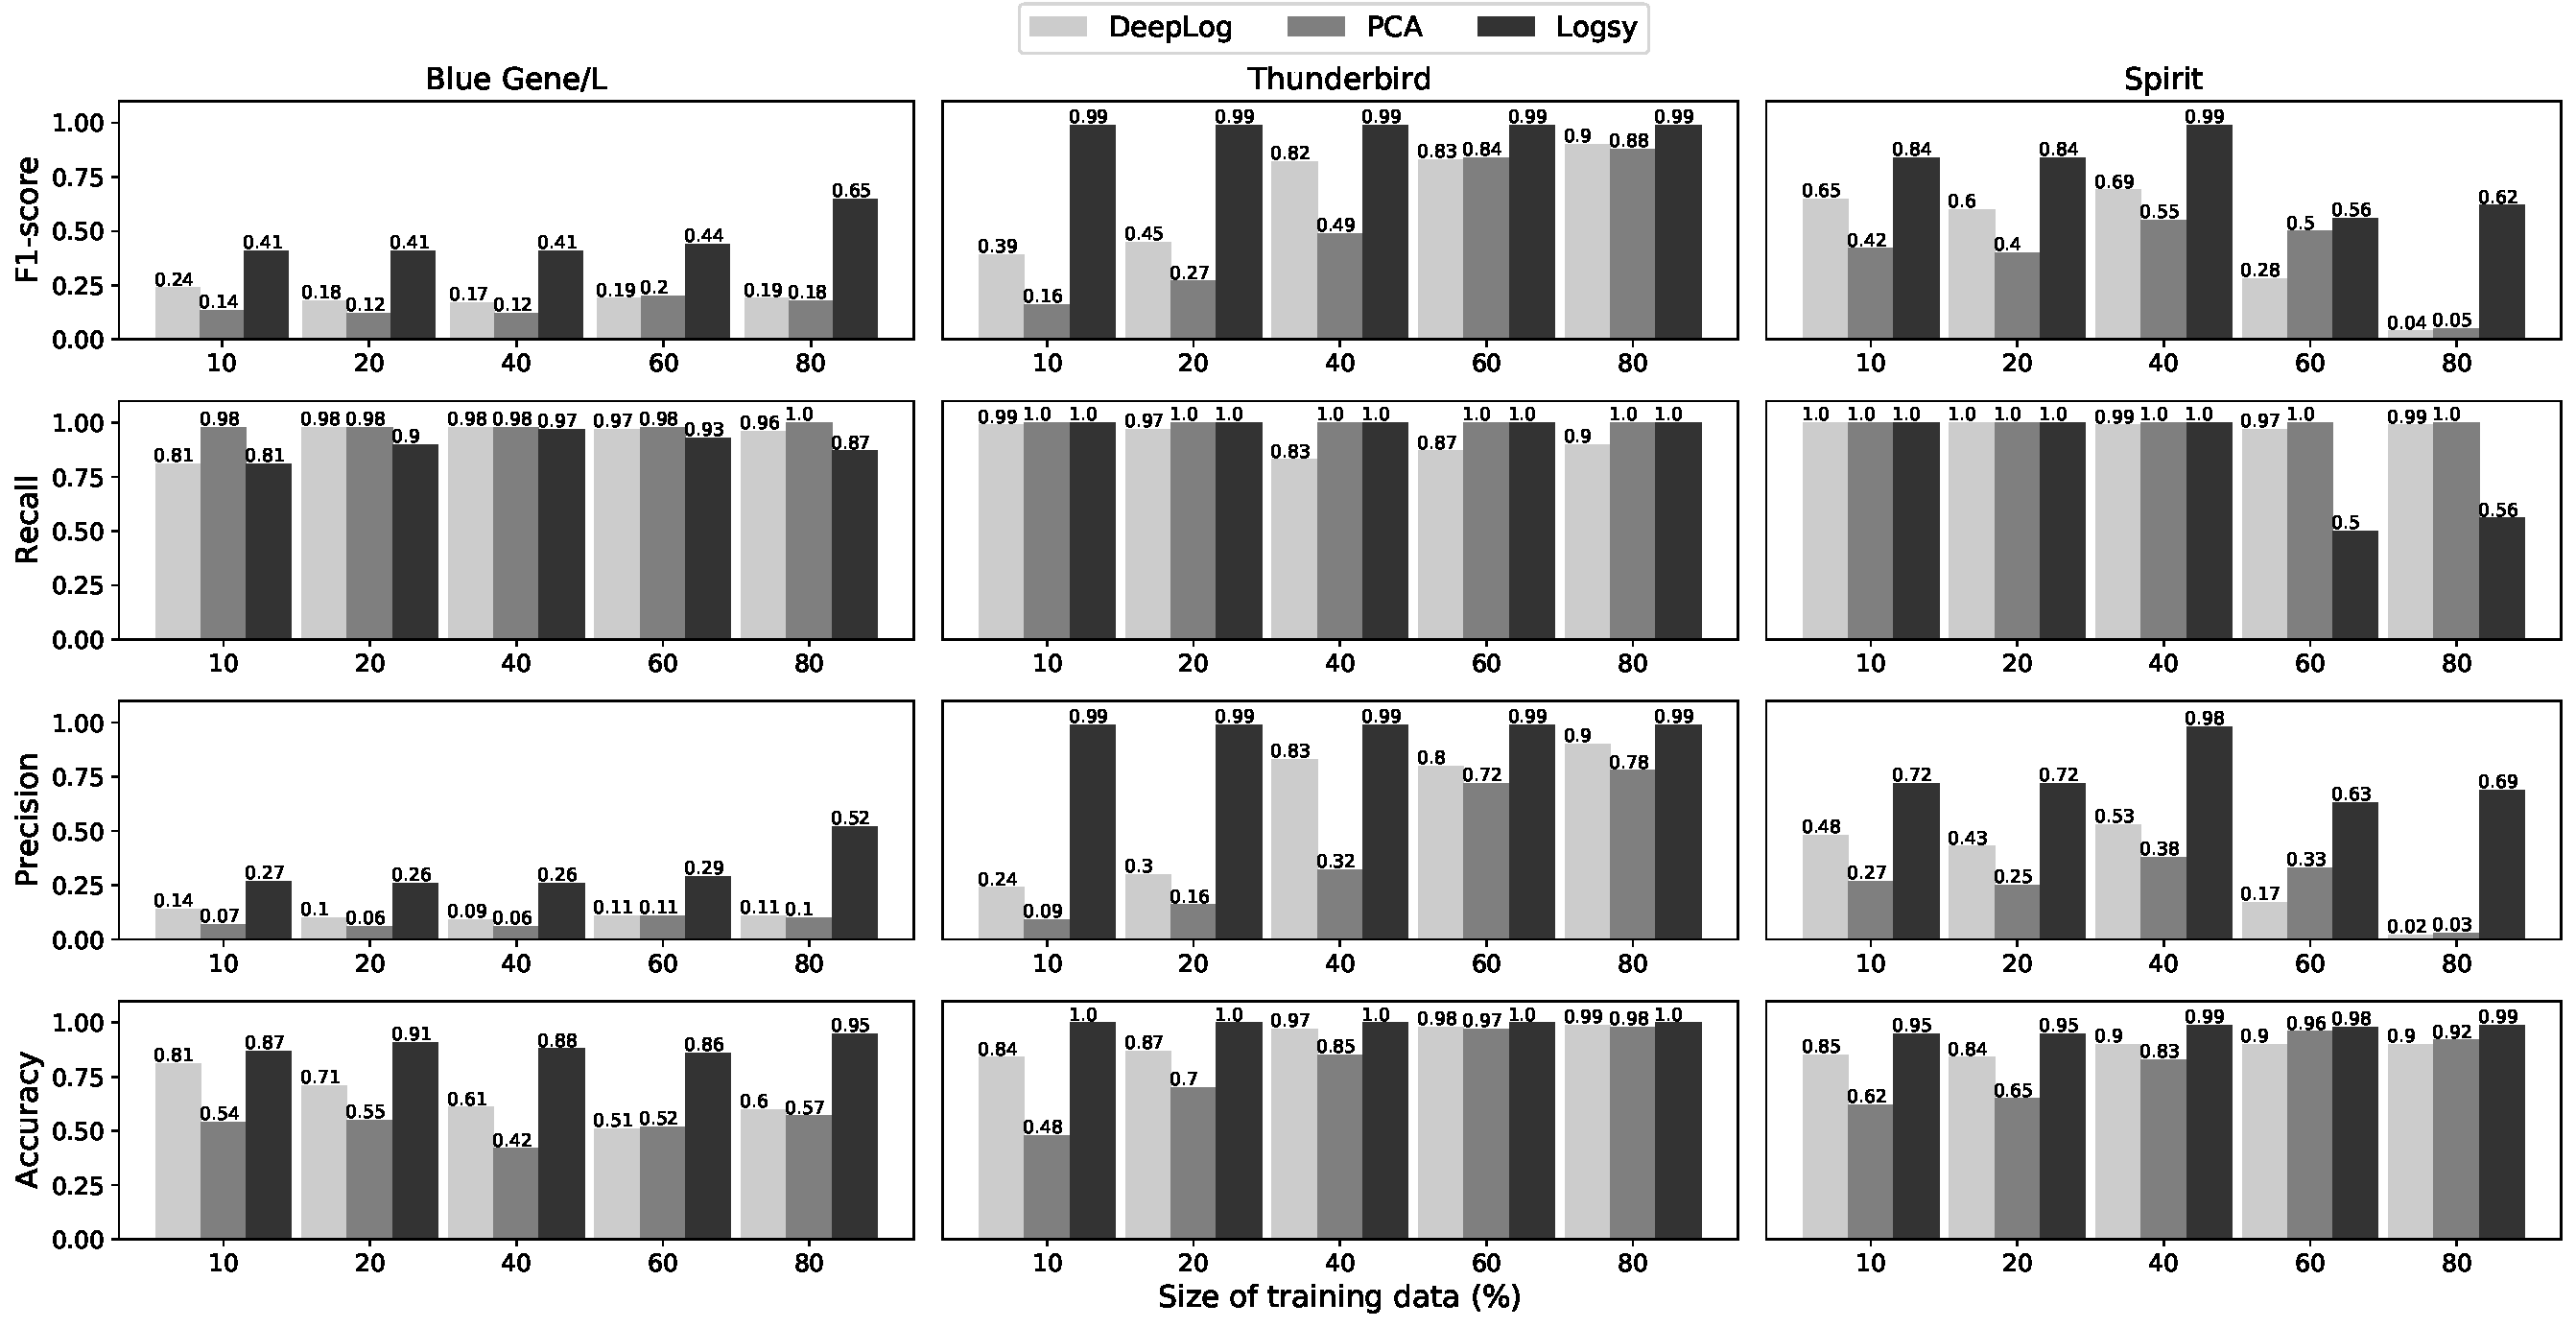
\includegraphics[width=1.0\textwidth]{gfx/chap4/results.pdf}
    \caption{Comparison of the evaluation scores against the two baselines DeepLog and PCA on three different datasets.}
    \label{fig:results}
\end{figure*}


\subsection{Results and discussion}
We show the overall performance of Logsy compared to the baselines in Figure~\ref{fig:results}. Generally, Logsy achieves the best scores, with an averaged F1 score in all splits of 0.448 on the Blue Gene/L dataset, 0.99 on the Thunderbird dataset, and 0.77 on the Spirit data. DeepLog and PCA have lower F1 scores in all performed experiments. The baselines have a very high recall, but low precision. This implies that they can find the anomalies. However, they will produce large numbers of FP predictions. 

Logsy preserves the high recall across the datasets and evaluation scenarios. In addition, it exhibits a large improvement in the precision scores, owing to the correct classification of new unseen log messages and reduction in the FP rate. For example, on the Blue Gene/L dataset, DeepLog and PCA exhibit 2--4 times lower precisions than that of Logsy. Overall, Logsy is the most accurate method with an average of 0.9. If a log anomaly detection method generates too many false alarms, it will add a too high overhead to the operators and large amount of unnecessary work. Therefore, high-precision methods are favorable. DeepLog leverages the indices of log templates, which ignore the meaning of the words in the log messages, to learn the anomalous and normal patterns. However, different templates having different indices can share common semantic information and both could be normal. Ignoring this information leads to the generation of FP for DeepLog compared to Logsy.
Notably, the increase in the training size also increases the F1 score for almost all methods, except for the last two splits in Spirit. These splits have very small numbers of anomalies. Notably, Logsy outperforms the baselines even when only 10\% of the data are training data. For example, in Blue Gene/L, we obtain an F1-score of 0.32 on 10\% training data, while the largest F1-score of the baselines is 0.24. In Thunderbird, this difference is even more noticeable, where an F1-score of 0.99 is already achieved with the first 10\%. This shows that even with a small amount of training data from the target system Logsy extracts the needed information on the reason responsible for the log message to be normal or anomalous. Logsy produces accurate predictions even in unseen samples.


\begin{figure*}[!t]
\minipage{0.33\textwidth}
  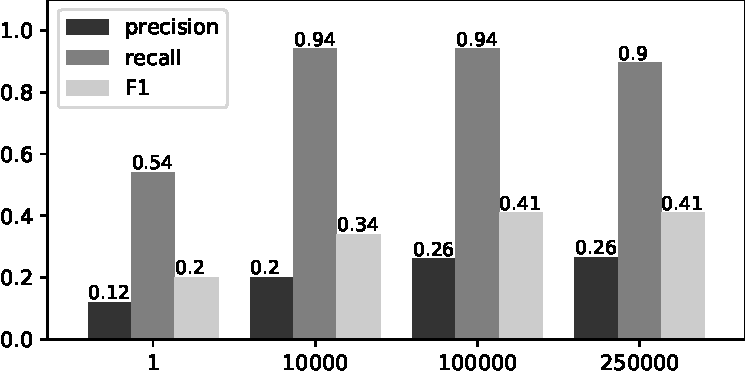
\includegraphics[width=\linewidth]{gfx/chap4/auxiliaryeffects.pdf}
\endminipage\hfill
\minipage{0.33\textwidth}
  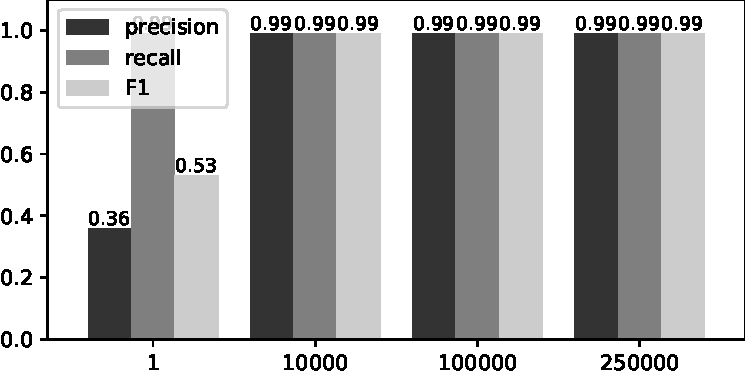
\includegraphics[width=\linewidth]{gfx/chap4/auxiliaryeffects_tbird.pdf}
\endminipage\hfill
\minipage{0.33\textwidth}
  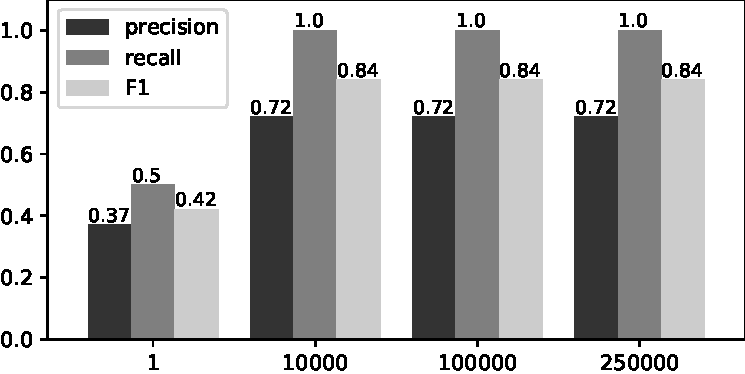
\includegraphics[width=\linewidth]{gfx/chap4/auxiliaryeffects_spirit.pdf}
\endminipage
\caption{Effect of the size of the auxiliary dataset. The target systems are Blue Gene/L, Thunderbird, and Spirit (left, middle, and right, respectively); 20\% train -- 80\% test split.}
\label{fig:auxiliary}
\end{figure*}

\subsubsection{Effect of the auxiliary data on the evaluation scores}
In this experiment, we perform an analysis of the Logsy performances with various sizes of the auxiliary data. We evaluate the same target vs. auxiliary data split for all datasets. We evaluate the approach on the 20\%--80\% train/test split. The results are shown in Figure~\ref{fig:auxiliary} for all datasets. The auxiliary data size increase from 1 to 250000 led to increases in all evaluation scores. With the increase in the size of the auxiliary data from 100000 to 250000, the scores do not change in both cases. This shows that the amounts of information present in the auxiliary data are similar and that all cases are already present in 100000 random samples. Notably, only one auxiliary sample, which may be even artificially generated, sufficiently acts as a regularizer to the hypersphere loss function. This prevents the model from learning trivial solutions. Increasing the variety of data (e.g., including more diverse log datasets) further improves the performance, owing to the increased number of samples representing abnormality.



% \begin{figure}[htbp]
%     \centering
%     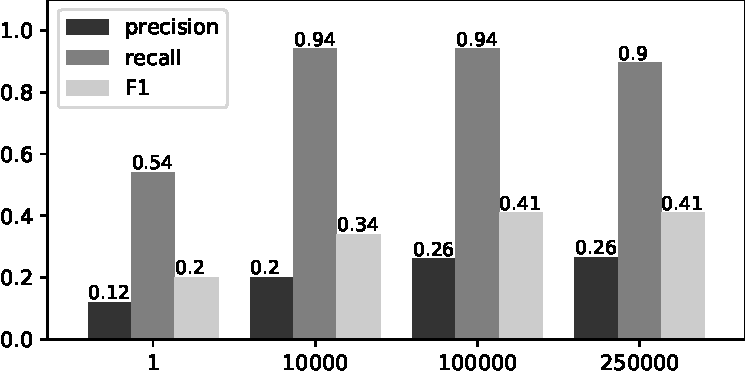
\includegraphics[width=0.99\columnwidth]{gfx/chap4/auxiliaryeffects.pdf}
%     \caption{Increasing the size auxiliary dataset, where the target system is the Blue Gene/L (20\% train - 80\% test)}
%     \label{fig:auxiliary_bgl}
% \end{figure}


% \begin{figure}[htbp]
%     \centering
%     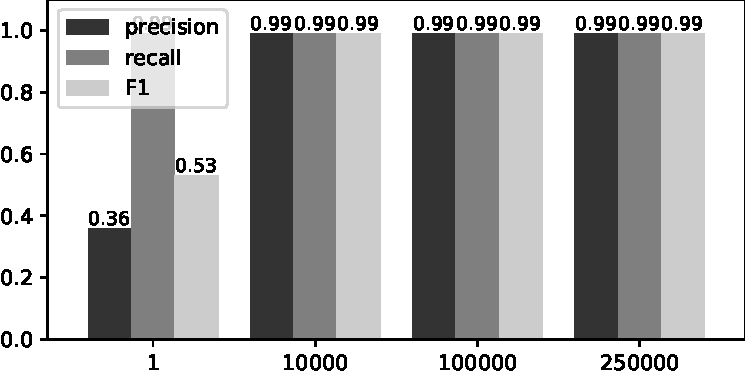
\includegraphics[width=0.99\columnwidth]{gfx/chap4/auxiliaryeffects_tbird.pdf}
%     \caption{Increasing the size auxiliary dataset, where the target system is the Thunderbird (20\% train - 80\% test)}
%     \label{fig:auxiliary_tbird}
% \end{figure}

% \begin{figure}[htbp]
%     \centering
%     \includegraphics[width=0.99\columnwidth]{gfx/chap4/auxiliaryeffects_spirit.pdf}
%     \caption{Increasing the size auxiliary dataset, where the target system is the Spirit (20\% train - 80\% test)}
%     \label{fig:auxiliary_spirit}
% \end{figure}


\begin{figure}[!htbp]
\centering
\includegraphics[scale=0.7]{gfx/chap4/semisupervised.pdf}
\caption{Effect of the increase in the size of the labeled anomaly data in the Blue Gene/L dataset (20\% train -- 80\% test).}
\label{fig:semisupervised}
\end{figure}


\subsubsection{Inclusion of expert labeling}
Often, systems are operated by humans, experts with system-specific knowledge. Sometimes, they could provide or manually label samples to improve the performance of the model. We experiment with the incremental inclusion of anomaly labels of the target dataset to test the model behaviour. We experiment on the 20\%--80\% split of the Blue Gene/L dataset. 
Figure~\ref{fig:semisupervised} shows the results. The increase in the number of labelled anomaly samples improves the performance. For as few as 2\% labelled data, we already obtain the best F1-score of 0.8. This shows that the addition of few percentages of anomalies as labelled samples to Logsy largely improves the performance. This only strengthens the hypothesis where the log anomaly detection must be addressed by understanding the reason responsible for the log message to be normal or anomalous. The labelled anomalies from the target system provide information utilized by Logsy to learn the differences between the normal and anomalous logs on the target dataset.


\begin{figure}[!b]
\centering
\includegraphics[scale=0.8]{gfx/chap4/tsne_BGL.pdf}
    \caption{Visualisations of the log vector representations of Blue Gene/L with T-SNE~\cite{maaten2008visualizing}.}
    \label{fig:tsne}
\end{figure}

\begin{figure}[!t]
\centering
   \includegraphics[scale=0.8]{gfx/chap4/thunderbird_distance.pdf}
    \caption{Distance of the log vector representations to the center of the hypersphere $\mathbf{c=0}$. The threshold is represented by the dashed line.}
    \label{fig:distance}
\end{figure}

\subsubsection{Utilization of the learned log embeddings in related approaches}
Representation learning is fundamental to obtain good performances of the machine learning methods~\cite{bengio2013representation}. In this experiment, we extract the learned log message vector representations from the already trained Logsy. To illustrate the vector representations of the logs, in Figure~\ref{fig:tsne}, we show their lower-dimensional representation of the test split through the T-SNE dimensionality reduction method~\cite{maaten2008visualizing} on the Blue Gene/L dataset. We show that the log vector representations are structured in a manner following the definition of our spherical loss function (see Section~\ref{vectorrepresentations}). The normal samples are concentrated around the centre of a hypersphere, which is a circle in two dimensions. Most of the anomalies are dispersed in the space outside the sphere. By assigning a threshold on the anomaly score $A(x_i)$, i.e., the distance from the centre of the sphere (circle), we can obtain a good performance. The same effect is observed on the Thunderbird dataset illustrated in Figure~\ref{fig:distance}, where we plot the distances of the test log vector representations to the centre of the sphere. The dashed line represents the optimal threshold for anomaly detection.  


\begin{figure}[!t]
    \centering
    \includegraphics[scale=0.9]{gfx/chap4/pcaembeddings.pdf}
    \caption{F1 score comparison of the standard PCA~\cite{xu2009detecting} and PCA using the embeddings extracted from our method (80\%--20\% split).}
    \label{fig:pcaembeddings}
\end{figure}



To illustrate the importance of the log embeddings, we perform experiments where we replace the original TF-IDF log representations in PCA~\cite{xu2009detecting}, as the lowest-performance method, with the extracted embeddings from Logsy. We show the results in the bar plot in Figure~\ref{fig:pcaembeddings}. The replacement of the log representation improves the performance of the PCA. Improvements in F1 score of 0.09, 0.11, and 0.01 were obtained for Blue Gene/L, Thunderbird, and Spirit, respectively. This demonstrates that the log representation learning has an impact, not only in Logsy, but also in previous approaches that could be adapted to use the new log embeddings. The relative improvement in F1 score, on average, is 28.2\%.


\begin{figure*}[!htbp]
\minipage{0.5\textwidth}
  \includegraphics[width=1.0\textwidth]{gfx/chap5/logsyspeedgputrain.pdf}
\endminipage\hfill
\minipage{0.5\textwidth}
  \includegraphics[width=1.0\textwidth]{gfx/chap5/logsyspeedgputest.pdf}
\endminipage
\caption{Speed performances of Logsy: training (left) and test (right) times.}
\label{fig:speedlogsy}
\end{figure*}


\subsubsection{Logsy: speed performance analysis}
To show that Logsy can be used in production in near-real-time settings, we evaluate its speed performance. The experiments were performed on a GPU NVIDIA 1660Ti (6GB) and CPU Intel(R) Core(TM) i7-9750H CPU at 2.60 GHz. Figure~\ref{fig:speedlogsy} shows the times needed for training and testing as functions of the data size. The figures show linear dependencies on the size of the log data. To analyze 3 million log lines, Logsy requires approximately 850 s for training and approximately 12 s for prediction. The prediction time is important in production settings, where less than $4 \mu s \mathrm{per log line}$ is required to predict each log line (obtained by dividing 12 s by 3 million log lines).


\section{Related work}
Extensive studies on the research and development of automated log analysis methods have been published in both industry and academia~\cite{zhu2019tools, he2016evaluation,shang2014log}. We provide an overview of the related studies on log parsing and log anomaly detection tasks.

\subsection{Log parsing}
Parsing techniques can be distinguished by various aspects, including technological, operation mode, and preprocessing. In Figure~\ref{fig:taxonomyparsing}, we present an overview of the existing methods.

\begin{figure}[htbp]
\centerline{\includegraphics[width=1.0\textwidth]{gfx/chap4/figure_parser_taxonomy.pdf}}
\caption{Taxonomy of log parses according to the underlying technology.}
\label{fig:taxonomyparsing}
\end{figure}


\textbf{Clustering} The main assumption in these methods is that the message types coincide in similar groups. Various clustering methods with proper string matching distances have been used. Methods in this group include SHISO, LenMa, LogMine, LKE, LogSig~\cite{mizutani2013incremental, shima2016length,hamooni2016logmine, fu2009execution, tang2011logsig}. Other parsing methods such as POD-Discovery~\cite{imweber2015}, are found in process mining, which utilize regular expressions and leverages the Levenshtein distance to separate variable and constant parts of the logs.

\textbf{Frequent pattern mining} assumes that a message type is a frequent set of tokens that appear throughout the logs. The procedures involve creating frequent sets, grouping the log messages, and extraction of message types. Representative parsers for this group are SLCT, LFA, and LogCluster~\cite{xu2009detecting, nagappan2010abstracting, nandi2016anomaly}.


\textbf{Evolutionary}. Its member MoLFI~\cite{messaoudi2018search} uses an evolutionary approach to find the Pareto optimal set of message templates.

\textbf{Log-structure heuristic methods} produce the best results among the different used techniques~\cite{zhu2019tools,he2016evaluation}. They usually utilize different properties that emerge from the structure of the log. The state-of-the-art algorithm Drain~\cite{he2017drain} assumes that, at the beginning of the logs, the words do not largely vary. It uses this assumption to create a tree with a fixed depth, which can be easily modified for new groups. In this group there are as well other related parsers such as IPLoM, and AEL~\cite{xu2009detecting, jiang2008automated}.

\textbf{Longest common subsequence} uses the longest common subsequence algorithm to dynamically extract log patterns from incoming logs. The most representative parser is Spell~\cite{du2016spell}.

The proposed method NuLog belongs to a new category referred to as \textbf{Neural} in the taxonomy of log parsing methods. Different from the current state-of-the-art heuristic-based methods, our method does not require any domain knowledge. Through empirical results, we show that the model is robust and applicable to various log types in different systems.

\subsection{Log anomaly detection}

Similarly to the log parsing, extensive studies have been published on the research and development of methods for log anomaly detection in both industry and academia~\cite{bodik2010fingerprinting, jakublogs,chen2004failure,farshchi2015experience,fu2009execution, hamooni2016logmine, liang2007failure, du2017deeplog, xu2009detecting,  zhang2019robust, meng2019loganomaly, nedelkoski2020selfsupervised,xu2014weber}. Out of those, the older methods utilize traditional statistical and machine learning models, and human intervention in the model creation, while the current studies focus on utilizing the large amounts of log data and mostly apply deep learning models.

Numerous supervised methods have been applied to address the log anomaly detection problem. For example, Liang et al.~\cite{liang2007failure} applied a support vector machine (SVM) classifier to detect failures, where both normal and anomalous samples are assumed to be available. Similarly, Chen et al.~\cite{chen2004failure} utilized the decision tree to model the logs from the targeted application. 
Brier et al.~\cite{breier2015anomaly} provided an overview of these supervised and more traditional approaches to log anomaly detection. Recently, LogRobust~\cite{zhang2019robust} and HitAnomaly~\cite{huang2020hitanomaly} provided supervised methods on sequences of log data and state-of-the-art results. However, as explained above, obtaining system-specific labeled samples is costly and often practically infeasible. Therefore, we discuss unsupervised methods below.

Several unsupervised learning methods have been proposed. Xu et al.~\cite{xu2009detecting} proposed using the PCA method, where they assumed different sessions in a log file that can be easily identified by a session-id attached to each log entry. It groups log keys by session, and then counts the appearances of each log key value inside each session. A session vector has a size of $n$, representing the number of appearances for each log key in $K$ in that session. A matrix is formed where each column is a log key, while each row is one session vector. PCA detects an abnormal vector (a session) by measuring the projection length on the residual subspace of a transformed coordinate system. The publicly available implementation enables a TF-IDF representation of the log messages, which is utilized in our experiments as a baseline. Lou et al.~\cite{lou2010mining} proposed invariant mining (IM) to mine the linear relationships among log events from log event count vectors. 

Log anomaly detection methods based on one-class classification~\cite{Zhang2016AutomatedIS,Vinayakumar2017LongSM} learn a model that describes the normal system behavior, usually assuming that most of the unlabeled training data are not anomalous and that anomalies are samples outside the learned decision boundary. The massive log data volumes in large systems have renewed the interest in the development of one-class deep learning methods to extract general patterns from nonanomalous samples. We classify these methods into the traditional group of methods, which leverage log parsing~\cite{nedelkoski2020selfsupervised, he2017drain} and follow the traditional log anomaly detection pipeline described in Figure~\ref{fig:parsingreferenceanomaly}. The formulated task is to predict the next index of the log template in the sequence $x_{h+1}$ by utilizing the history of template vectors (count, one-hot encoding) $H=x_0,\dots,x_h$, as for DeepLog~\cite{du2017deeplog}.

Some studies have leveraged NLP techniques to analyze log data based on the fact that log is a natural language sequence. Zhang et al.~\cite{Zhang2016AutomatedIS} proposed to use the LSTM model and TF-IDF weight to predict the anomalous log messages. Bertero et al.~\cite{bertero2017experience} used word2vec and traditional classifiers, such as SVM and Random Forest, to evaluate whether a log event is an anomaly. Similarly, LogAnomaly~\cite{meng2019loganomaly} incorporates pretrained word vectors for learning of a sequence of logs; they trained an attention-based Bi-LSTM model.

Furthermore, in the process-based modelling literature there are number of methods that also consider anomaly detection from log data as sequential problem. Xu et al.~\cite{xu2014weber} use log data to extract operational activities such as upgrade, redeployment, and on-demand scaling and perform anomaly detection to increase the system dependability. The authors proposed Process Oriented Dependability (POD)-Diagnosis, an approach that explicitly models these
sporadic operations as processes. These models allow to determine orderly execution of the process, use the process context to filter logs, trigger assertion evaluations, visit
fault trees, and perform on-demand assertion evaluation for online anomaly detection. In the same direction, several other studies from process-based anomaly detection~\cite{nolle2020process,PECCHIA2020105054,nolle2016unsupervised,nolle2018analyzing,nolle2019binet,imweber2015,xu2014weber,rehse2020} make use of sequential log events to mine processes and detect anomalies. In these studies, log data is often associated with having trace ID, where log events are related, and activities are extracted to bridge the gap from raw log events to the process mining methods. On the other hand, we view the log events as independent samples, and analyze them from the point of natural language processing, and text anomaly detection. We draw more concrete comparison to these methods in the trace analysis chapter.

The learning of the sequence of template indices and enhanced log message embedding approaches still have large limitations in terms of generalization for previously unseen log messages. They tend to produce false predictions owing to the imperfect log vector representations. For example, learning sequence of logs represented by indices cannot correctly classify newly appearing log messages, as the new log will be an out-of-boundary index. The domain where the word vectors are pretrained (e.g., Wikipedia) has essential differences from the language used in computer system development. To partly mitigate some of these limitations in unsupervised approaches, one approach is to incorporate labeled data from operators and perform life-long learning~\cite{du2019lifelong}. However, it still requires frequent periodical retraining, updates, and costly expert knowledge to label the data, without addressing the problem of generalization on unseen log messages that appear between retraining epochs. 

Different from the above methods, we used the interpretation of the anomaly detection as binary classification between normal and anomalous points. We utilized the concept reported by Steinwart et al.~\cite{steinwart2005classification} that the bias on the anomalous distribution is crucial for an improved detection. We provided such bias by employing easily accessible log datasets as an auxiliary data source. 

\section{Chapter summary} \label{conclusion}
Logs are an important data source for anomaly detection in computer systems~\cite{zhu2019tools, du2017deeplog, zhang2019robust}. In this chapter, we described the traditional pipeline for log anomaly detection. Most methods utilize log parsing as the first step toward anomaly detection. We identified limitations in existing parsing methods, including the use of regular expressions, heuristics (e.g., the variable parts of the log message appear near the end of the log message~\cite{he2017drain}), and multiple hyperparameters for tuning~\cite{zhu2019tools,du2016spell,hamooni2016logmine}. As the anomaly detection depends on the parsing, the accuracy of the log parsing directly affects the effectiveness of the log anomaly detection. Therefore, we presented a method, NuLog, to mitigate these limitations and improve the overall effectiveness of the methods. NuLog addressed the log parsing problem by deep language modelling. Words appearing at a constant position of a log record implies that their correct prediction can be directly used to produce a log message type. An incorrect prediction indicates that a token is a parameter. 
We carried out experiments on 10 real-world log datasets and evaluated the method against 12 log parsers from a public benchmark. The experimental results showed that NuLog outperforms the existing log parsers in terms of accuracy, edit distance, and robustness. In addition to the parsed templates, NuLog produces log vectors. We analyzed the effectiveness of using the log vectors directly for anomaly detection. In the analysis, we compared the NuLog log vectors with the state-of-the-art log anomaly detection method and anomaly detector trained in a supervised manner. The NuLog's log vectors improve the anomaly detection. However, we identified a large gap between the efficiency scores, favoring the supervised learning. The unsupervised approaches still led to large numbers of FPs. 

To bridge the gap between supervised and unsupervised anomaly detection methods, we identified the log vectors as a main issue in previous methods~\cite{he2017drain,du2016spell,meng2019loganomaly,zhang2019robust,du2017deeplog}. The main drawback is the prediction of unseen log messages owing to the evolution of logging statements, system updates, and processing noise. 

To overcome this problem, we presented a new anomaly detection approach, Logsy. Logsy shifts from the traditional log anomaly detection pipeline and does not utilize an external log vector computation. In contrast, it learns end-to-end log vectors and predicts anomaly scores. It is based on a self-attention encoder network with a new hyperspherical classification objective. We formulated the log anomaly detection problem in a manner to discriminate between normal training data from the system of interest and samples from auxiliary easy-access log datasets from other systems, which represent an abnormality.

We presented an experimental evidence that our classification-based method Logsy exhibits a high performance for deep anomaly detection. Logsy outperformed the baselines by an F1 score margin of 0.25. Logsy can efficiently include available expert labels. Furthermore, the log vector representations from Logsy are meaningful and generally can be utilized in other methods. Using PCA to utilize the log vectors from Logsy, we obtained an improvement in the F1 score of 0.07 (28.2\%). 

The preference for unsupervised learning in previous log anomaly detection studies is reasonable for the traditional settings, which often lack access to out-of-distribution samples that are representative examples of anomalous data. Owing to the large amount of easily obtainable log data, it is reasonable to assume that access to anomaly data informative for detection is available. We hypothesize that future research on deep log anomaly detection should focus on classification with anomalous auxiliary data and development of approaches to incorporate domain bias for the diversity of normal and anomaly data. 

 % Chapter 5
% Chapter X

\chapter{Anomaly Detection in Distributed Tracing Data} % Chapter title
\label{ch:traces} % For referencing the chapter elsewhere, use \autoref{ch:name} 
\minitoc
\bigskip

Distributed traces contain information about the execution workflow and performance at a service level within the system. The trace representation, noise, large number of services, complex service relationships between them, arbitrary lengths, and lack of labels pose difficulties for the anomaly detection methods~\cite{liu2020unsupervised}. In this chapter, to address these challenges, we introduce a sequential representation of the trace. This helps utilize various methods for anomaly detection in sequential data. We describe a baseline approach based on sequence prediction with LSTMs to perform anomaly detection~\footnote{Based on our early study on trace anomaly detection using deep learning~\cite{nedelkoski2019anomalymultimodal}}. This modeling approach has several advantages and limitations, identified in this chapter. We reformulate the learning task from sequence prediction to prediction of missing parts of the trace. This helps preserve the major advantages of sequential trace representation and increase the robustness to previous limitations such as the noise and degraded performance on larger traces. Finally, we demonstrate the ability of the method for root-cause localization, i.e., finding the contribution of each of the services within the trace to the decision whether the trace is anomalous.

This chapter includes the following contributions~\footnote{Parts of this chapter are published in ~\cite{nedelkoski2019anomalymultimodal,nedelkoski2020data,nedelkoski2019anomaly,nedelkoski2020selftracing} and a patent is filed in~\cite{nedelkoski2020patentjasmin}.}.
\begin{itemize}
    \item We compile the trace structure as a text sequence, which provides possibilities for applications of deep learning methods.
    \item We introduce a baseline deep learning approach based on LSTMs.
    \item We present a problem formulation for anomaly detection in distributed tracing and method based on self-supervised learning, denoted as Tracy.
    \item We demonstrate an approach to utilize the model to track the differences between the normal and abnormal traces. This leads to an improved reasoning for the root cause analysis and localization of the services with downgraded performances.
\end{itemize}

\section{Sequence learning for trace anomaly detection}
In this section, we start with transformation of the trace to a textual representation and describe the preprocessing steps needed for the model learning phase. We present a baseline LSTM-based approach and derive key benefits and drawbacks. These insights are utilized to reformulate the autoregressive problem definition and design Tracy, a self-supervised trace anomaly detection method. 

\subsection{Trace preprocessing}
Traces are produced by a program that executes a set of logic and control functions, following certain patterns and grammar rules on which the system operates. If the spans of the trace are sorted by time, the graph-like trace structure can be expressed as a finite sequence, $T=(S_1, \dots, S_m)$. We transform and compile the trace to such representation and provide an analogy to the natural language. A trace can be related to a sentence, the events/spans inside a trace to words, and the causal relationship between events to a language grammar (e.g., relations between words).

\begin{figure}[!htbp]
\centerline{\includegraphics[width=1.0\textwidth]{gfx/chap6/tracepreprocessing.pdf}}
\caption{Preprocessing of the trace.}
\label{fig:tracepreprocessing}
\end{figure}

As the spans contain an additional meta-information, they have to be parsed to obtain a uniform structure, before they can be effectively used for anomaly detection~\cite{nedelkoski2019anomaly}. The parsing, similar to that for logs, uses raw spans as an input and generates a template. Thus, the trace can be represented as a sequence of template indices.

In Figure~\ref{fig:tracepreprocessing}, we show the parsing procedure of the trace's spans. Depending on the span type (e.g., initiated from RPC or HTTP request), we select only the most important part properties. They, in the example of HTTP request, are the name of the method (e.g., GET), HTTP status code, URL, and service name. The importance of the properties is related to their informativeness. Properties that are different in each span, e.g., the ID of the span, are not considered as informative properties.

Considering the large variability of the URLs, owing to mostly the IDs inside them, the number of different spans can be very large, leading to difficulties in modeling. As most of these span's URLs representing one service differ solely in the identifiers (e.g., the ID 12939fd is ID of the image), we replace them with $\langle * \rangle$ through parsing and extract span templates or groups. To this end, we use a log parsing method (NuLog). At this point, the trace is represented as a sequence of span templates. As traces can contain repetitive spans, to preserve the start and end of the trace, we add two additional spans to the beginning and end of the trace ([START] and [STOP]). 

The third step in the prepossessing is the creation of a lookup table where the templates that are output from the parser are mapped to a specific index. Thus, each span is mapped to an index and the trace is a sequence of indices. To consider the possibly different lengths of the traces, the traces are padded up to $max\_len$. This parameter represents the maximum allowed trace length. This makes the traces equally sized. The data format at the output of the preprocessing has a shape of $D_1 = (N_t, max\_len)$, where each row is a trace $T_i = \{x_1^i,x_2^i,\dots, x_{max\_len}\}$, $N_t$ is the number of all recorded traces, and $x_j^i \in \mathbb{V}$ are indices from the dictionary. 

\begin{figure}[!t]
\centerline{\includegraphics[width=1.0\textwidth]{gfx/chap6/lstmprocesstrace.pdf}}
\caption{LSTM network architecture for trace anomaly detection.~\cite{nedelkoski2019anomalymultimodal}}
\label{fig:lstmtraceprocess}
\end{figure}

\subsection{Autoregressive LSTM-based method for anomaly detection}
To perform anomaly detection, we start by modeling the normal system behavior. We model the transition probability from a sequence of spans into the next in-sequence span
\begin{equation}
     P(x_t=l_i|\{x_{t-h}, \dots, x_{t-2}, x_{t-1}\}),
\end{equation}
where $P$ is the conditional probability of the next span for given input
recent sequence of $h$ spans within the trace and $l_i \in L=\{l_0, l_1, \dots, l_{N_l}\}$ is the index from the dictionary of spans. The conditional probability can be modeled with an RNN, e.g, LSTM/GRU. We show the architecture of the approach in Figure~\ref{fig:lstmtraceprocess}.

The input to the model are the indices from the spans. Each $x_t$ is fed as an input in the corresponding timestep $t$. The output at $t$, for the current inputs $\{x_{t-h}, \dots, x_{t-2}, x_{t-1}\}$, is a probability distribution over the $N_l$ unique labels from $L$. 
Every LSTM block at $t$ is composed of $H$ LSTM cells. 
It has a memory state that encodes all information from the previous timesteps together with the input fed at the same timestep.

The vertical stacking of layers is a common practice to achieve better results by extracting highly-abstract features~\cite{Hundman:2018:DSA:3219819.3219845,vincent2010stacked}. The model's parameters are optimized by minimizing the categorical cross-entropy loss between the predicted span and ground truth.

During the prediction time, if we are unable to successfully predict a certain number of next spans (more than a specified threshold), the trace is considered anomalous; otherwise, it is normal.

\subsection{Limitations of autoregressive approaches}
The LSTM-based method belongs to the autoregressive approaches. Thus, it has several inherit limitations including (1) forward context is not considered during the modeling phase~\cite{devlin2018bert}. Thus, the model does not utilize the full trace information. (2) Lack of robustness to noise and trace length variability, owing to the inability of autoregressive models to preserve long interdependencies between the services (e.g., the span on the first position is related to the span on the 100-th position of the trace). Moreover, as mentioned above, the sequential representation of the trace is obtained using the initially graph-like trace structure. Therefore, this representation does not preserves all initial information. 

A desired behavior of the model would be to learn additional interdependencies between the spans in the trace, other than the sequential. The model, to preserve the graph information within the sequence, needs to extract dependencies between distant spans in the sequence. For example, as depicted in Figure~\ref{fig:interdependenciessequential}, the model needs to be able to infer that span A is related to span K, which have long-term dependencies. To address these limitations of autoregressive models, we reformulate the learning task and present a novel method, Tracy.


\begin{figure}[!t]
\centerline{\includegraphics[width=1.0\textwidth]{gfx/chap6/interdependenciessequential.pdf}}
\caption{Long term interdependencies.}
\label{fig:interdependenciessequential}
\end{figure}


\section{\textit{Tracy}: self-supervised anomaly detection in distributed traces}
Each span's position within the trace is dependent on the other spans (can be located at any position) in the trace~\cite{sigelman2010dapper,RepTrace,chow2014mystery}. The contextual information is related to the likelihood of occurrence of a particular span on a position within that trace. The set of spans used to pinpoint the location of another span is referred to as context of the span. Intuitively, it is reasonable that deep models, e.g., Bi-LSTM~\cite{huang2015bidirectional}), are strictly more powerful than either a left-to-right (autoregressive) model or shallow concatenation of left-to right and right-to-left models. However, standard conditional models can only be trained left-to-right or right-to-left, as bidirectional conditioning would allow each word to indirectly "see itself" and the model could trivially predict the target word in a multi-layered context, which would lead to over-fitting.

\begin{figure}[!t]
\centerline{\includegraphics[width=1.0\textwidth]{gfx/chap6/overviewtracy.pdf}}
\caption{Overview of Tracy.}
\label{fig:tracyarchitecture}
\end{figure}

To train a contextual representation of the spans and trace from both forward and backward contexts, in Tracy, we mask a percentage of the input spans at random, and then predict the masked tokens (see Figure~\ref{fig:tracyarchitecture}). To this end, Tracy learns the likelihood of appearance of particular span with given context spans. We utilize this as a proxy task for anomaly detection, which we refer to as masked span prediction (MSP), similar to MLM in~\autoref{ch:logs:logparsing}. With such a learning task, we model the traces representing the normal behavior of the system. In the prediction phase, if a trace is normal, the success rate of correct prediction of the masked spans with given context spans will be high; otherwise, the success rate will be low, suggesting an anomalous trace. Thus, introducing a threshold on top of the success rate of correctly predicting the masked spans within the trace is utilized to decide whether the trace is anomalous or normal. 

To solve the MSP task, we use the transformer encoder neural network architecture. It is based on the attention learning concept, which, in the context of traces, relates the input spans to given target (masked span). The underlying learning mechanism (self-attention~\cite{vaswani2017attention}) enables the target to be selective on which spans are relevant. In the case of traces, this allows a sparse representation. It enables the trace to be represented with only the spans that are core and must appear in normal traces, minimizing the effects of the noisy spans. In other words, it builds abstract span representations that contain information for short and long interdependencies. Formulating the problem of trace anomaly detection as MSP enables to capture the complete end-to-end execution path among all involved components of the system. 


\begin{figure}[htbp]
\centerline{\includegraphics[width=1.0\textwidth]{gfx/chap6/exampleTracesMask.pdf}}
\caption{(Top) Example of \textit{network create and delete trace}. (Bottom) Example of the context of the \texttt{POST /v3/auth/tokens/} span used for the input of the self-attention mechanism. \textit{POST /v3/auth/tokens/} is denoted as masked span.}
\label{fig:exampletrace}
\end{figure}

The step after preprocessing is to perform masking. We illustrate the masking of an example trace in Figure~\ref{fig:exampletrace}. In the bottom line of the image, the \textit{POST /v3/auth/tokens/} span is replaced by the \texttt{[MASK]} span. A masked span in a trace can be any randomly chosen span that during the learning procedure is labeled with a special \texttt{[MASK]} span from the input. During the learning procedure, the true value of the masked token is used as a target and predicted by the remaining spans that construct the context (used as an input). This enables the masked span to "score" the relevance of the spans from the context for its prediction. With the span masking procedure, we produce training samples for every masked span. For example, if we mask two spans of a trace $T$, the masking module will produce two traces, each having one masked span. This enables one trace to be replicated multiple times and different contexts for the spans of traces from different workloads to be learned. Moreover, such masking of the spans that leads to various contexts for prediction of a span acts as a regularization technique to improve the robustness~\cite{devlin2018bert}. Intuitively, noisy spans that appear infrequently will be masked only few times, in contrast to spans that are frequent. Whenever a previously unseen normal trace from a known user request is presented to the method, according to the described property, the self-attention mechanism will be less sensitive to the changes that appear owing to noisy spans. Thus, the masking and self-attention mechanism enforce the model to focus on learning to attend core spans that appear in the trace.

After the masking procedure, the trace is modified to  
\begin{equation}
    T_{i}^{preprocessed}=([START], S_1^i, S_2^i, \texttt{[MASK]}, \dots, S_{T_{max\_len}}^i, [STOP]),
\end{equation}
and as such is utilized as an input to the neural network.

\begin{figure}[!t]
\centerline{\includegraphics[width=1.0\textwidth]{gfx/chap6/tracymultihead.pdf}}
\caption{Neural network architecture used to solve the MSP task.}
\label{fig:msptracy}
\end{figure}

Figure~\ref{fig:msptracy} depicts the model's architecture. It is an encoder--decoder structure that maps the input spans in a vector format, learns higher-level abstract representations, and projects them to a probability distribution over the vocabulary of spans. The encoder uses a multi-head self-attention mechanism as a basic building block. 

The processed inputs are fed into the network. To preserve the sequential information, each span is encoded with an additional position value. Formally, this block calculates a vector that maintains the relative position of a span within a trace. Similar to the positional encoding in the log data (\autoref{ch:logs:logparsing}), the positional encoding block implements this by adding periodic functions (e.g., sine and cosine) to the vector representations of the spans in the trace.

The multi-head attention block is a neural network architecture, which implements the self-attention mechanism~\cite{vaswani2017attention}. It operates by projecting the input context for the masked span into various subspaces and aggregating them. Each projection is controlled by one of the $L$ heads of the multi-head attention. The multi-head block uses three vectors, key, query, and value, as an input. It uses the key and query of the current input representation to assign scores for the context spans from the trace to the current masked span. Intuitively, this part learns the influence of the context spans on the prediction of the masked spans. 
% As the multi-head attention block was already described in detail in \autoref{ch:logs}, we skip additional mathematical formalities.

The next part of the network consists of two feed-forward layers. They provide a richer representation of the underlying output of the multi-head attention mechanism. The outputs are fed through a one-layer network with softmax at the end, which serves as a decoder. The softmax is used as a function to generate probabilities over the whole dictionary of spans. These probabilities suggest the likeliness of the current masked span to be associated with a symbol within the vocabulary of symbols conditioned on the context. 

\subsection{Detecting anomalies}
The MSP is a proxy task for anomaly detection. As a standalone task, it cannot be used for anomaly detection. To this end, we introduce an additional postprocessing of the predictions of the MSP model to detect anomalies. The output from the MSP for a particular trace and masked span is an ordered list of predictions as possible spans for the masked position in the trace. The lists are ordered according to their relevance (probability) to be the particular masked span. During the anomaly detection, each of the ordered lists on the particular position in the trace is analyzed in the following manner. If the observed value on a particular position of the trace is not in the first $top-k$ elements of the list generated by the MSP task module for that position, we consider the span as incorrect. We count the errors for each trace and divide their number by the trace length forming the ratio of misclassified examples or span error rate per trace. The span error rate serves as an anomaly score. If a model leads to many mistakes, the anomalous score is higher, and thus the trace is anomalous. Setting a decision threshold on the anomaly score can be used to decide whether the trace is normal or anomalous. The span error rate is another key characteristic of the method that addresses the noise in the traces. In the following section, we empirically demonstrate the validity of these claims.

\newpage

\section{Evaluation}
In this section, we describe the data utilized for the evaluation. We describe the learning scenarios (LSs) used to evaluate the performance of our method and present the results. We investigate the differences in the attention scores between the normal and anomalous traces and their utilization to infer characteristic differences between the normal and anomalous traces.

\subsection{Experimental data}
We evaluated the presented method on two separate datasets, a dataset from a planet-scale industry system (referred to as production data) and dataset generated from our testbed deployment. The experiments were performed on a GPU NVIDIA 1660Ti (6GB) and CPU Intel(R) Core(TM) i7-9750H CPU at 2.60 GHz.

\textbf{OpenStack~\cite{ShrivastwaOpenstack} testbed.} It is based on a microservice architecture, running in a dockerized environment Kolla-Ansible~\cite{kollaansible}. OpenStack was deployed on four compute and one control nodes. 

The normal and anomalous data are generated by the execution of three workloads. (1) \textit{Create and delete server} uses a task from Rally~\cite{rally} to create and delete a VM. The fault is injected in a compute node, which restarts the API container that runs on the compute nodes. (2) \textit{Create and delete image} uses the \textit{glance} project of OpenStack to create and delete an image. The faults are injected by restarting the glance-API, which runs on the controller node. (3) \textit{Create and delete network} is a an operation that provides a network interface. The anomaly is injected by disruption of one of the neutron services (e.g., neutron metadata agent, neutron server) during the creation of a network.

To represent a scenario close to the real world, the workloads are executed concurrently. As some operations are faster than others (e.g, we need more time to boot a machine than to create a network), the workloads are performed with different numbers of iterations. 2000, 3000, and 6000 iterations for create and delete server, create and delete image, and create and delete network were carried out, respectively. The injections of the faults were carried out at every 250 iterations for \textit{create and delete server} and \textit{create and delete image} and every 500 iterations for \textit{create and delete network}. After the execution of the sequence of workloads, reports for the conducted experiments are generated. The reports contain details for the successful execution of the workload. They are used to induce the ground truth label for a particular user request. This is needed to separate the normal from anomalous traces to perform the evaluation.

\textbf{Production data}. Even in small controlled experimental setups, the noise is high and the traces change over time. This already poses challenges for the anomaly detection. However, testing the approach on large-scale production cloud data is required to show the viability of the approach. It covers traces from the creation of a VM upon request from the user. A characteristic property of production traces is their significantly larger length than those of the experimental testbed. The production data available in this experiment contained 200 traces with different lengths. 

\begin{figure}[htbp]
\centering
\includegraphics[width=1.0\textwidth]{gfx/chap7/traceanomalyinjections.pdf}
\caption{Anomaly injection scenarios in trace data.}
\label{fig:traceanomalyinjections}
\end{figure}


\subsection{Learning scenarios}
To evaluate and compare the performances and robustness of the proposed attention method and state of the art in anomaly detection from tracing data, we consider three LSs (see Figure~\ref{fig:traceanomalyinjections}). To test the ability of Tracy to preserve the global and local properties within the traces, we grouped our experiments into three groups (short, long, and combined (short and long) traces). The definition of these categories is data-driven, which implies that short traces are considered those that are concentrated around the lower values of the trace lengths ($\leq median$). The remaining traces belong to the category of long traces. 

\textbf{Real anomalies (LS1)}. In this LS, in the test set, the anomalies generated by the deployed testbed were used. The aim of this scenario is to evaluate the performances of the methods for anomaly detection from tracing data in the presence of anomalies generated by the system.

\textbf{Artificial anomalies (LS2)}. The anomalies in the traces are usually reflected by shortened traces, according to the procedure that generates the anomalies. Restarting a service interrupts the trace at particular span. The anomalies can be injected at every span in the trace as every span represents a service that can be malfunctioning. To evaluate the generalization and robustness of the method scaling to different types of anomaly, a set of artificial anomaly tests is created. The creation of this set is carried out in a manner that $L$ traces from the normal test set are selected at random. The selected traces are truncated at random position. These traces are labeled as anomalous and are joined with the remaining normal traces to create the test set.  


\textbf{Span permutation (LS3).} Owing to various reasons (e.g., an increased number of user requests or caching), some of the traces may have different orders of appearance of the spans, but still complete the whole operation, which implies that the trace is normal. In this LS, the test data are constructed as follows. First, a random selection of a normal trace is carried out. Second, a random span is permuted with its right neighbour, if existing. Third, this procedure is repeated for $L$ randomly selected traces composing the test set. In the test set, only normal traces exist.

We selected the best parameter configuration in LS1 and used it to evaluate the method in all LSs, LS1, LS2, and LS3. This enables to directly evaluate the changes in the performances of the methods to novel anomalies and random permutation in the neighbours, which reflects the ability of the method to handle traces with noise. To demonstrate the independence of the performance of the method on the position of the injected anomaly, we carry out an additional robustness test. During this test, 500 randomly selected traces among the normal traces are sampled. In each trace at each position, one of the spans is replaced by a randomly chosen span, while treating the changed trace as an anomaly. The experiments are repeated five times to obtain estimates for the expected performance score and its confidence intervals. 

\subsection{Baselines}
We compare Logsy against two publicly available methods, (1) LSTM-based trace anomaly detection~\cite{nedelkoski2019anomalymultimodal}, proposed in our earlier study and explained previously, and (2) TraceAnomaly~\cite{liu2020unsupervised}, a state-of-the-art method based on deep Bayesian networks with posterior flows. TraceAnomaly processes each trace as a whole to construct a service trace vector that encodes the invocation path. It then learns the overall normal trace patterns for a service during offline training. Lastly, in online anomaly detection, for each new trace, an anomaly score is computed, and accordingly traces with small anomaly scores are considered anomalous. As TraceAnomaly largely outperforms other more traditional methods such as string matches or finite state machines, we discard direct comparisons to these methods in our evaluation. The parameters of the LSTM-based method and TraceAnomaly are tuned to produce their best F1 scores.

\subsection{Results}
We present the results of the three LSs, including the precision, recall, and F1 score.

\begin{figure}[!t]
\centering
\includegraphics[width=1.0\textwidth]{gfx/chap6/ls1.pdf}
\caption{Results of the experiments for LS1.}
\label{fig:LS1}
\end{figure}

Figure~\ref{fig:LS1} shows the results of LS1 for the best-selected models from the optimization. When the long traces are considered, higher scores are obtained for the attention mechanism than those of the previous state-of-the-art methods, LSTM and TraceAnomaly, in all three cases. The attention mechanism can prioritize specific spans of the trace owing to the sparsity characteristic. Thus, the attention mechanism utilizes the most salient spans that form the trace. On the contrary, the LSTM-based method focuses on local properties of a trace owing to the autoregressive assumption. TraceAnomaly leads to problems in noise handling (e.g., changes in few spans), responsible for most false predictions. The comparable performances on the short traces are obtained as all methods utilize the locality in the traces. The largest advantage of Tracy over the state-of-the-art methods originates from the log traces. The performance of Tracy remains high even when traces are long. The precision for long traces outperforms the baselines by 0.3 owing to the reduction in number of false positive predictions. The good performance on the combination of the long and short traces for all methods (F1 above 0.9) is attributed to the imbalance dataset, where the number of short traces is considerably larger.

\begin{figure}[!t]
\centering
\includegraphics[width=1.0\textwidth]{gfx/chap6/ls2.pdf}
\caption{Results of the experiments for LS2.}
\label{fig:LS2}
\end{figure}

Figure~\ref{fig:LS2} shows the results of LS2. We observe a notable decrease in the recall for both small and long traces in LSTM and TraceAnomaly. This implies that, in this scenario, the baselines tend to produce an increased number of false negatives. This can be explained as the anomalous trace differs from the normal only in its length, owing to the inability of the methods to extract global patterns from the trace. The methods exhibit good performances for short traces and lower performances for longer traces. Long traces are more common in large distributed systems as they contain hundreds of services~\cite{nedelkoski2019anomaly}. Executing one operation in a microservice architecture includes invoking multiple services not necessarily only HTTP calls for the communication between the services. Hence, the ability to handle long traces is imperative for applicability in tracing data from real-world systems. 


\begin{figure}[!t]
\centering
\includegraphics[width=1.0\columnwidth]{gfx/chap6/sensitivity_analysis.pdf}
\caption{Sensitivity analysis of Tracy vs. LSTM.}
\label{fig:3}
\end{figure}

\begin{figure*}[!t]
\centering
\includegraphics[width=1.0\textwidth]{gfx/chap6/positiontracy.pdf}
\caption{Performance score estimates with respect to the position of the injected anomaly. The solid line represents the mean value of the F1 score, while the shaded region is the confidence interval of one standard deviation.}
\label{fig:8}
\end{figure*}


LS3 evaluates the generalization ability of the method. Figure~\ref{fig:3} shows the results of \textit{LS3}. As it is a one-class prediction scenario, only the accuracy of correctly predicting the normal iterations is presented. This LS can be interpreted as testing the ability of the method to correctly predict novel normal traces that occur owing to the noise. The attention method is more robust than TraceAnomaly and LSTM. The cases of wrong classification in Tracy are mostly due to swapping of one of the "core" spans in the trace. Thus, the attention method cannot correctly predict the masked span. Nevertheless, on average, across all traces, the number of core spans for given trace is small, and thus the presented method exhibits a better score. LSTM and TraceAnomaly detect almost every change, which limits their noise robustness. However, TraceAnomaly has a higher noise tolerance than that of LSTM, achieving higher scores. 

To further evaluate the robustness of Tracy, in Figure~\ref{fig:8}, we show the F1-score with respect to the position of the injected anomaly. For the short traces (until 12 spans), the performances of the attention and LSTM-based methods are high and they are robust regarding the position of the inserted change. However, for long traces, a higher sensitivity of the LSTM-based method to small local changes within the trace is observed. This leads to a lower performance. These results show that the position of inserting a swap does not influence the performance of Tracy. The larger variance observed in the figure for the long trances is attributed to the small number of long traces in the training data. TraceAnomaly exhibits comparable performances to those of Tracy, as it also utilizes the global trace information.



\begin{table}[!t]
\centering
   \caption{Results for the production data from a global service provider.}

   \label{tab:1}
   \begin{tabular}{lrrrr}
     \toprule
     Dataset & Accuracy & Precision & Recall & F1  \\
     \midrule
     Production data & 0.92 & 0.91 & 0.95 & 0.93    \\
     \bottomrule
   \end{tabular}
\end{table}

\tablename~\ref{tab:1} summarizes the results for the production data. The method evaluation was performed by a global service provider to reduce the evaluation bias. Therefore, the experiments for the baselines were not performed. Tracy exhibits a high F1 score of 0.93, consistent with the results of the testbed evaluation. It demonstrates the usability of the proposed method for long noisy traces from a production setting. The analysis of the missclassified traces showed only small changes toward the last spans. 

\begin{figure}[!b]
\centering
\includegraphics[width=0.55\columnwidth]{gfx/chap6/euc_distance.pdf}
\caption{Distributions of the distances of attention scores between the normal--normal (black) and normal--abnormal (red) traces.}
\label{fig:4}
\end{figure}


\subsection{Explanation of decisions}
The attention scores in the context of the MSP task are weights indicating the influence of each span of the trace on the prediction of the current masked span. These scores can be plotted in a heatmap and form a fingerprint. The spans that have the largest influence form a trace identifier. Figure~\ref{fig:4} shows the distribution of Euclidean distances of attention scores between normal traces (in black) and distribution of distances between the normal and abnormal traces (in red). A separation between the distributions can be observed. The distances between the normal and abnormal score matrices are larger. This suggests that observing the anomalous and normal self-attention scores can be utilized to indicate anomalous spans, which point out to anomalous services.

Figure~\ref{fig:5} shows the squared errors of the self-attention scores between normal and anomalous traces, where positions 2 and 4 are corrupted, respectively. An increased error at the particular position within the attention score matrix where the span was corrupted was observed. This indicates that the cross comparison between the normal and anomalous attention scores provides insights into the potential causes of the anomaly. In these examples, the deviations in the attention scores from the normal traces are emphasised at positions 2 and 4 of the trace. This shows that these positions are very unlikely to be occupied by the corrupted span. The operator can track the properties of this span and relate them to a potential cause.


\begin{figure}[!t]
\centering
\includegraphics[width=1.0\columnwidth]{gfx/chap6/tracefingerprint.pdf}
\caption{Squared difference between the attention scores of normal and abnormal traces when an anomaly is injected at position 2 (left), 4 (right). The brighter color indicates larger scores.}
\label{fig:5}
\end{figure}


% \begin{figure}[!t]
% \centering
% \minipage{0.45\columnwidth}
%   \includegraphics[width=1.0\columnwidth]{gfx/chap6/img.pdf}
%   \caption{Squared difference between the attention scores of normal and abnormal traces when an anomaly is injected at position 2. The brighter color indicates larger score values.}\label{fig:5}
% \endminipage\hfill
% \minipage{0.45\columnwidth}
%   \includegraphics[width=1.0\columnwidth]{gfx/chap6/img2.pdf}
%   \caption{Squared difference between the attention scores of normal and abnormal traces for injection position 4.}\label{fig:6}
% \endminipage
% \end{figure}

\begin{table}[!t]
\centering
   \caption{Results of the correct localization of the inserted positional anomalies.}
   \label{tab:2}
   \begin{tabular}{lrrrrr}
     \toprule
     Position & 1 & 2 & 3 & 4 & 5 \\
     \midrule
     Correct prediction [\%] & 0.93 & 0.95 & 0.94 & 0.90 & 0.88    \\
     \bottomrule
   \end{tabular}
\end{table}


Furthermore, we replaced each position of the trace obtained by the execution of a \textit{create and delete} network request by random span. We computed the accuracy of correct span localization. Table~\ref{tab:2} summarizes the results. The attention scores can indicate the positional differences between normal and anomalous executions of a trace and thus locate the anomalous span.

\section{Related work}
Recently, extensive studies have been carried out on anomaly detection using tracing data. The straightforward approach for trace anomaly detection is based on string matching. For example, if a distributed system handles a user request by generating the sequence events/symbols $S_{1} = [M, N, O, Y, P]$, this sequence can be compared to a set of known sequences $S_{i}, \forall i\in \{0,\dots, N\}$, which represents the valid behavior of the system. If the sequence is found, the request is processed successfully. If sequence $S_{1}$ is not found, we can assume that a failure or anomaly occurred during the handling of the user request. However, the underlying volatility of the distributed system, as described in ~\autoref{ch:concepts:sec:anomalydetectionindistributedsoftwaresystems:subsec:trace}, makes the problem more complex than simple matching.

Three important requirements for anomaly detection from distributed traces exist. As described in \autoref{ch:concepts:sec:anomalydetectionindistributedsoftwaresystems:subsec:trace}, the methods should handle traces under the assumption of presence of noise, arbitrary lengths, and absence of labels.


\begin{figure}[htbp]
\centerline{\includegraphics[width=1.0\textwidth]{gfx/chap7/cacheasidepattern.pdf}}
\caption{Caching and its effect on traces.}
\label{fig:cacheasidepattern}
\end{figure}

For example, noise can be caused by caching in distributed systems. It leads to suppression of symbols in traces as some instructions are not executed when the result is cached (see Figure~\ref{fig:cacheasidepattern}). Thus, a model can contain the following observed traces, [M, N, P, Q], [M, P, Q], and [M, N, Q]. When a new trace [M, Q] needs to be tested, it is intuitive that it is an anomaly as it was not seen in the past. Nonetheless, if we assume that the system under analysis can generate traces with noise, it is not obvious whether [M, Q] is an invalid trace or valid trace containing noise. The existing approaches, such as that in \cite{RepTrace}, use finite state machines (FSMs) to model the correct behaviors of systems. These approaches exhibit high performances when the traces do not contain noise. However, the introduction of noise scales the number of potential transitions exponentially. Thus, modeling noise using FSM-based approaches is not feasible as it will be possible to only model the already observed noise.

Approaches relying on LSTMs, e.g., those in our early study on an LSTM-based trace anomaly detection~\cite{nedelkoski2019anomalymultimodal,nedelkoski2019anomaly}, can process only traces up to a certain length of $k$. These approaches are referred to as autoregressive as they use previous symbols of a trace to predict the following symbol. For example, the developed techniques test the trace [M, N, P, Q, R, S] by predicting which symbol is after C according to a behavioural model, [M, N, P, Q, R]. If the prediction is correct (Q), the trace is classified as normal. Otherwise, it is anomalous. However, as traces become long, LSTMs are not capable of establishing a correlation between head symbols (M, N) and tail symbols (R, S). The first symbols of traces in a behaviour model are forgotten. This implies that the predicted symbol does not depend on all previous symbols. To address this limitation, approaches have been refined to use a sliding window with a size $< k$ over long traces. This strategy may improve the results but does not solve the problem that the symbols of a head trace are not considered by the prediction. 
The second drawback in these approaches is related to the production of more erroneous predictions because they observe only a fixed number of previous events to predict the upcoming event. Such models do not utilize the existing relation between distant spans in the trace. They learn the normal system behaviour from partial and limited data from previous events, which might affect the overall performance.

Recently, a new method denoted as TraceAnomaly~\cite{liu2020unsupervised} uses deep Bayesian networks to automatically learn the overall normal patterns of traces during periodic offline training. In online anomaly detection, a new trace with a small anomaly score (computed based on the learned normal pattern) is considered anomalous. TraceAnomaly, similarly to Tracy, utilizes global properties of the traces using variational inference. We identify the noise handling as the strongest drawback of TraceAnomaly owing to the lack of mechanism that prioritizes particular spans of the traces.

Lastly, methods from process-based anomaly detection~\cite{nolle2020process,PECCHIA2020105054,nolle2016unsupervised,nolle2018analyzing,nolle2019binet,imweber2015,xu2014weber,rehse2020} are related similarly. Weber et al.~\cite{imweber2015} describe two systems. The first, PODDiscovery, simplifies the creation of such an abstract process model (related to model of a trace) from operations logs. The proposed approach performs large amount of previously manual steps automatically, drastically reducing the time needed for obtaining the process model. Using the discovered model, the second system, PODViz, provides operators with the ability to visualize the current state of an operations process in near-real-time, and to replay a set of events to understand how the process context changed over time. There are several differences to the presented method--Tracy, namely, PODViz involves human interaction and obtains abstract representation from event logs into activities, which are related into a trace. On the other hand, Tracy performs end-to-end learning and detection of anomalies from the raw trace events. Nolle et al.~\cite{nolle2020process,nolle2016unsupervised,nolle2018analyzing,nolle2019binet} proposes process anomaly correction. This approach combines the benefits of conformance checking and process anomaly detection. Given a trace, the process anomaly correction detects anomalous executions, indicates where the anomaly has occurred during the execution, and suggests possible corrective measures. Similar to Tracy, the proposed approach employs deep learning. It defines the task of understanding the processes via learning to predict the next activity in a process. The resulting machine learning model thus represents an approximation of the real process that created the data. Therefore the approach is closely related to the LSTM based method presented in above, and the TraceAnomaly, which are part of the evaluation in this thesis. To that end, the drawn differences about these methods are as well aligned for the process-based anomaly detection methods.

\section{Chapter summary} \label{conclusion:traces}
This chapter addressed the problem of anomaly detection in large-scale distributed systems as an essential task for their security and reliability. We addressed the problem by introducing a new learning task, MSP, for the problem of execution-path anomaly detection from tracing data. The novel definition of the problem enables to include information from the entire trace, directly utilizing the existing service relations. It provides higher predictive performances in the problem of structural anomaly detection, particularly for the long traces, than those of other existing approaches for tracing data based on LSTM. Empirically, we showed that the proposed approach is more robust against small permutations in the normal traces, a scenario frequently occurring in practice. The experiments showed that the method has a high performance for experimental testbed data and in real production settings for a large cloud provider. Lastly, through the self-attention scores, we showed an approach to visualize and explore traces, showcasing important spans and differentiation from normal to anomalous traces.
 % Chapter 6
% Chapter X

\chapter{Multi-source detection of complex anomalies} % Chapter title
\label{ch:joint} % For referencing the chapter elsewhere, use \autoref{ch:name} 
\minitoc% Creating an actual minitoc\
\bigskip

In the previous chapters, we presented methods for anomaly detection related to each of the observability components. However, as standalone detectors from the corresponding data source, they have a limited view on the system. In this regard, insights gleaned from a combination of different observability signals are necessary to properly troubleshoot distributed systems~\cite{sridharan2018distributed}.

In this chapter, we analyze whether the full observability of the system, i.e., recording metrics, logs, and traces, provides exposure of the broader spectrum of anomalies. The contributions presented in this chapter are summarized below~\footnote{Parts of this chapter are published in ~\cite{nedelkoski2020data,nedelkoski2020jointmodalities,nedelkoski2019distributions}.}. 

\begin{itemize}
    \item We provide an analysis of complex anomalies in distributed software systems and their reflection in the observability components.
    \item A heuristic for detection of one of three system health states (normal, degradation, and failure state) is described by utilizing the data sources affected by an anomaly.
    \item By presenting case studies of complex anomalies, we show that a rule-based integration of the anomaly detectors helps broaden the spectrum of possible anomalies that can be detected. 
    \item We open-source the testbed and multi-source data, available on Zenodo~\footnote{https://zenodo.org/record/3549604}.
\end{itemize}

\section{Complex anomalies in distributed systems}
Often referenced reasons in various failure analysis studies on distributed software systems are attributed to deployments, exceeding scaling limits, infrastructure changes, and various system and software failures~\cite{sillito2020failures}. We relate them with the properties of the  distributed systems, particularly with the heterogeneity, scalability, and concurrency. 

The heterogeneity in the distributed systems implies complex pieces of code that stick together different resources, written in potentially different programming languages. Consequently, software bugs are unavoidable. Often, in software upgrades, a small configuration change in a system component can be overlooked. This can lead to failures of the system component. As the components (e.g., services) in a distributed system communicate through the network, it is highly likely that the anomaly will affect other system components. 

Prior to the system deployment in production, numerous tests are executed to evaluate the functionality of the system, e.g., under various loads. However, particular limits of the system are infeasible to be tested. Exceeding the scaling limits is one of the causes for failures in the systems. Examples include the rapid increase in the number of concurrent user requests. It can be to a point where a component of the system is not scalable or a system may exhaust available resources, which
implies a resource leak. Thus, the concurrency and scaling of distributed software systems can strongly influence the appearance of complex anomalies.

\begin{figure}[!t]
\centerline{\includegraphics[width=1.0\textwidth]{gfx/chap7/complexanomalies.pdf}}
\caption{Complex anomalies in the Openstack use case.}
\label{fig:complexanomalies}
\end{figure}

The analyzed complex anomalies are anomalies that do not reflect in each of the observability data. For example, a possible anomaly could not be (or hardly) observed in metrics, but easily found in the logs. In the following use-case, we perform an experiment where specific anomalies are reflected only in different data sources. We consider a scenario as in Figure~\ref{fig:complexanomalies}, where the anomaly is originated from the failure in the networking infrastructure on a hardware level, which eliminates the access to the compute host. This anomaly propagates on a application level, where services are affected. Mainly the compute host is responsible for the creation of VMs. Depending on the severity of the problem of the networking infrastructure, the system will be in a degraded or failure state of operation, i.e, the compute service will have a decreased performance or will not be reachable. The right panel shows the metrics, logs, and traces. The top right image presents a model of a trace generated during the normal operation of the system and serves as a nominal value for comparison to the rest of the scenarios (degraded and failure). The plots in the center in gray show the normal distributions of the duration for performing the operation. The anomalous distribution times are presented in black. We assume that the operator has trained anomaly detectors available for all system data sources.

Over time, the client experiences a time of creation of VM longer than usual. However, the client files the first report stating "Longer time for performing an operation". The operator analyzes this report, consults the anomaly detector on the response time, and finds that the response time is larger. However, the observed response time value is in the overlap of the distributions of normal and abnormal duration times. The operator is not sure if he/she should implement further actions. If trace anomaly detection is available to the operator, he/she can immediately observe that the trace is structurally different, compared to the structure when the trace is normal. These differences can be visually observed in Figure~\ref{fig:complexanomalies}. 
The timely observation allows the operator to notice and react to an anomaly during the degraded state of the system. If the operator at this point in time consults the logs, no issue will be reported. This anomaly is not reflected in the structure of the logs, as the operation finishes successfully. Therefore, having the multiple perspectives of the system at disposal provides a higher visibility and supports the correction of false or uncertain predictions reported by a single model. In this case, the trace suggests an anomaly, while the anomaly is not easily observed in the logs and metrics.

In second case, the client issues another report stating "Cannot execute any operation". The consulting of the three modalities then clearly shows a failure, compared to the previous case of degraded state. In addition, according to the trace, most likely, the problem is in the api service as it cannot be contacted. This problem is also reflected in the log data, as shown in L1 and L2 in the figure. We confirm that particular anomalies in complex systems do not reflect in all data components. 

\begin{figure}[!b]
\centerline{\includegraphics[width=1.0\textwidth]{gfx/chap7/solution_overview.pdf}}
\caption{Triano overview.}
\label{fig:Triano}
\end{figure}

\section{\textit{Triano}: integration of the anomaly detectors}
To address the problem of detection of complex anomalies, we introduce a rule-based integration of the detectors, denoted as Triano (see Figure~\ref{fig:Triano}).

We consider three trained anomaly detectors, presented in the previous chapters, $f_m(\mathbf{x_m})$, $f_l(\mathbf{x_l})$, and $f_t(\mathbf{x_t})$ for the metrics, logs, and traces, respectively. The input data in (1) $f_m(x_m)$ are a time series representing a system metric $\mathbf{x_m}={x_m^{w_m}, x_m^{w_m}, \dots, x_m^{w_m}}$, where $w_m$ is the window size, in (2) $f_l(x_l)$ are a system log message $\mathbf{x_l}={x_l^1, x_l^2, \dots, x_l^m}$, where $x_l^i$ are $d-$dimensional representations of the words in the log message and $m$ is the number of words, and in (3) $f_t(x_t)$ are a trace $\mathbf{x_t} = {x_t^1, x_t^2, \dots, x_t^k}$, where $x_t^i$ is a span and $k$ is the number of spans in the  trace. 

Each of the separate methods for anomaly detection in metrics, logs, and traces outputs its predictions, either 0 (normal) or 1 (anomaly), in the following format.

\begin{itemize}
    \item Metano, the metric anomaly detector $f_m(\mathbf{x_m})$, outputs \textit{(start time, end time, prediction, description}. The start and end time are the timestamps of the start and end of the window from the metric time series, while the prediction and description are related to the state of the system (normal or anomalous) and recognized anomaly pattern, as presented in~\autoref{ch:metrics}, respectively.
    \item Logsy, the anomaly detection method for log data $f_l(\mathbf{x_l})$, outputs \textit{(timestamp, prediction)} whether the observed log message is normal or anomalous, as presented in~\autoref{ch:logs}.
    \item Tracy, the anomaly detection method for trace data $f_t(x_t)$, outputs \textit{(start time, end time, prediction)} where the start and end times are the timestamps of the start and end of the analyzed trace, as presented in~\autoref{ch:traces}, respectively.
\end{itemize}

On top of the outputs of the anomaly detection methods, a time window $w$ is utilized to aggregate the predictions for a final decision, whether a possible anomaly exists in the observed system. Formally, the final output at a time $t$ is $g_t(f_m, f_l, f_t, w)$, which  is 0 or 1. As we observe different frequencies of predictions, first, the data from all data sources are aligned according to the start of the trace. 

An example of forming the final prediction is described. The tracing data contain information about multiple services, and thus the trace anomaly detector is prioritized. If this method reports an anomaly, the result is an anomaly is present. If anomaly is not present in the traces, logs are checked (log anomaly detector). If the log module does not generate an anomaly, the metric module is consulted. However, as depicted in Figure~\ref{fig:Triano}, the  approach is modular and any improvement in each of the detectors will improve the overall framework. Moreover, it enables flexibility of assessments of the order of the data sources, as the operator may have an additional knowledge on the type of anomalies that may arise in the system of interest. The knowledge can originate from either experience or availability of other informative sources such as source codes and configuration files.

We additionally designed a more complex multimodal deep learning method for automatic integration, however there were only negligible differences to the rule-based approach (see~\autoref{appendixA}).

\section{Evaluation}
In this section, we analyze the performance of Triano against single methods. We describe the experimental testbed, data, three anomaly cases, and evaluation. 

\begin{figure}[!htbp]
\centerline{\includegraphics[width=1.0\textwidth]{gfx/chap7/testbedTriano.pdf}}
\caption{Experimental testbed.}
\label{fig:Trianotestbed}
\end{figure}

\subsection{Experimental testbed}
For the generation of the data, we deployed an OpenStack~\cite{ShrivastwaOpenstack} testbed based on a microservice architecture running in a dockerized environment denoted as Kolla-Ansible~\cite{kollaansible}.
OpenStack is a cloud operating system, which controls large pools of computing, storage, and networking resources throughout a data center. All of them are managed and provisioned through APIs with common authentication mechanisms.
The experimental testbed is shown in Figure~\ref{fig:Trianotestbed}. For the generation of the data, it consists of one control node and four compute nodes. It was deployed on bare-metal nodes of a cluster. Each node has a RAM of 16 GB, three 1-TB disks, and two 1-Gbit Ethernet NICs. Three hard disks were combined to a software RAID 5 for data redundancy.

To generate user workload and inject faults into the system, we used Rally\cite{rally}. To evaluate the approach in scenarios close to real-world workloads, we used a series of user actions: create user -> create image -> create network -> start VM -> stop VM -> delete VM -> delete network -> delete image -> delete user. 

For monitoring and data collection, we utilized Prometheus for the metric data~\cite{turnbull2018monitoring}. Elasticsearch, Logstash, and Kibana (ELK) were used to aggregate logs from all services running across the physical nodes. To export logs from Elasticsearch into CSV, a CLI tool, es2csv, was utilized. To collect the traces, we utilize OSProfiler~\cite{openstack}, which is used by all OpenStack projects and their Python clients to generate traces. It generates one trace per request. 

To enable evaluation of the framework and methods, labeled data are required. Different data types require different labeling types. To label the data, we use the standard procedure of employing domain expert. (1) For traces, we consult a domain expert to label whether the trace is an anomaly. The trace may be either completed or not. We investigate its structure if it differs in many events, compared to the normal before providing it with a label. (2) For the logs, we analyze each log message using regex searches and label it to produce a labeled set of data. Anomalous log messages may appear outside the period of injection of anomalies. It is also important to label those instances. For the metrics, we perform the labeling in a similar manner. All models are trained by utilizing data from the time intervals when the system is in a normal state. 

\begin{table}[htbp]
\caption{Description of complex anomalies.}
\label{tab:complexanomalies}
\resizebox{\columnwidth}{!}{%
\begin{tabular}{cl}
\hline
Type            & \multicolumn{1}{c}{Description}                                                                                                                            \\ \hline
Network failure & \begin{tabular}[c]{@{}l@{}}Networking failure in the host node eliminated the access \\ to the host, leading to multiple failures (system hardware)\end{tabular} \\ \hline
Service update  & \begin{tabular}[c]{@{}l@{}}Configuration change in system A led to failures in A’s\\ calls to system B (deployment)\end{tabular}                           \\ \hline
Service failure & \begin{tabular}[c]{@{}l@{}}Failure in the message queue left several queues locked, \\ blocking messages (system software)\end{tabular}                    \\ \hline
\end{tabular}
}
\end{table}

\subsubsection{Anomaly scenarios}
To evaluate the combined approach against the single methods, we injected the anomalies described in Table~\ref{tab:complexanomalies}. 
The first considered anomaly is a network failure anomaly. This anomaly eliminates the access to a host, which leads to multiple failures. The second anomaly arises during deployment. Changes in configuration of system A led to failures in A calls to system B. We resolve this problem with deployment with a correct configuration. The third anomaly is a service failure. The anomaly is injected into the message queue (MQ) and leaves several queues locked, which blocks the message flow. We resolve it by cleaning the queue and restarting the service. 

\subsection{Results}


\begin{table}[!t]
\caption{Network failure multi-source anomalies; log data.}
\label{tab:network:logs}
\resizebox{\columnwidth}{!}{%
\begin{tabular}{cl}
\hline
Type     & \multicolumn{1}{c}{Log message}                                                                                                                                                                                                                                                                                                                                                                                       \\ \hline
Normal   & \begin{tabular}[c]{@{}l@{}}L1. 130.149.249.132  POST /v2.1/os-server-external-events HTTP/1.1 status: 200 len: 582 time: 0.0948207. \\ L2. {[}instance: f2adf232-3c39-477f-af0c-db25c9e4b4d6{]} During sync\_power\_state the instance has a pending \\ task (spawning). Skip.\end{tabular}                                                                                                                           \\ \hline
Degraded & \begin{tabular}[c]{@{}l@{}}L1. DHCP configuration for ports \{'451c037f-83d7-4fa7-86df-0b8afdbab99c'\} is completed“. \\ L2. 130.149.249.132  GET /v2.0/ports?device\_id=3322a8e7 b233-4115-96e1-f98450f1c2d0 HTTP/1.1\\ L3. failed to flush the buffer. retry\_time=2  next\_retry\_seconds chunk=error\_class=Fluent::Plugin::\\ ElasticsearchOutput::RecoverableRequestFailure read timeout reached“.\end{tabular} \\ \hline
Failure  & \begin{tabular}[c]{@{}l@{}}L1. failed to flush the buffer. retry\_time=1  next\_retry\_seconds chunk error\_class=Fluent::Plugin::\\ connect\_write timeout reached“. \\ L2. Function “nova.servicegroup.drivers.db.DbDriver.\_report\_state’ run outlasted interval by 0.25 sec“.\end{tabular}                                                                                                                       \\ \hline
\end{tabular}
}
\end{table}


\begin{figure}[!t]
\centerline{\includegraphics[width=0.9\textwidth]{gfx/chap7/metricsnetworkfailiure.pdf}}
\caption{Network failure multi-source anomalies. Normal metric distribution (left), two degraded states (middle), and failure state (right).}
\label{fig:network:metrics}
\end{figure}


\textbf{Network anomaly.}
Figures~\ref{fig:network:metrics} and \ref{fig:network:traces} show the metrics and traces, while Table~\ref{tab:network:logs} shows the logs, for the normal and abnormal executions of the operations. We carry out a simultaneous analysis of the three sources.


Figure~\ref{fig:network:metrics} shows the distributions of the response time durations during the normal and abnormal executions of the operations. The durations are represented as distribution plots of the duration of the normal (blue) and duration of the anomalous (orange) operations. During the normal state, the duration has a bimodal distribution, with one mode around 450 s and another mode around 500 s. We observe normal traces and logs. However, cross comparison of the durations during the small degradation (the second column for the metrics and first row for the traces) shows that the structures of the trace are similar, but the response times are different. Suspicious logs are not observed. This degradation is a problem reflected in the duration time, but not in other modalities. Hence, the duration serves as a good indicator of potential problems in the system. In this case, the metric method detects this anomaly, while the log and trace anomaly detectors are not able to detect this problem, as it is absent in the data. The combined approach detects this degradation problem as it is reflected in the metric data. On the contrary, if the decision is based solely on the logs or traces, the degradation will be missed out. This could lead to potential failures. 

\begin{figure}[!t]
\centerline{\includegraphics[width=0.9\textwidth]{gfx/chap7/tracesnetworkfailiure.pdf}}
\caption{Network failure multi-source anomalies. Normal trace (top), degradation (middle), and failure state (bottom).}
\label{fig:network:traces}
\end{figure}

Increasing the severity of the anomaly leads to a significant increase in the response time (the third column in Figure~\ref{fig:network:metrics}). In addition, the trace anomaly detector detects an anomalous trace and a structurally different trace is observed, while the logs are still unable to record anything. Triano detects the anomaly in the traces and metrics simultaneously. 

Finally, when the network of the host has failed, the trace cannot be completed. In addition, the response time is very large and timeout log messages appear. Furthermore, the trace anomaly detector and analysis of the scores per span show that the major issue is in nova-api (Figure~\ref{fig:network:traces}), which is hosted on the failed host. The Triano framework can detect all degraded and failed states. 



\begin{figure}[!b]
\centerline{\includegraphics[width=0.9\textwidth]{gfx/chap7/serviceupdatemetrics.pdf}}
\caption{Service failure due to an update, multi-source anomalies, and metric data. Normal metric distribution (left), two degraded states (middle), and failure state (right).}
\label{fig:callservice:metric}
\end{figure}


\begin{table}[!t]
\caption{Service failure due to an update, multi-source anomalies, and log data.}
\label{tab:callservice:logs}
\resizebox{\columnwidth}{!}{%
\begin{tabular}{cl}
\hline
Type     & \multicolumn{1}{c}{Log message}                                                                                                                                                                                                                                                                                                                                                                                                            \\ \hline
Normal   & \begin{tabular}[c]{@{}l@{}}L1. {[}instance: 5d616cd-5689-44a0-8466-cf9290bff684{]} Instance spawned successfully. \\ L2. 130.149.249.132 - - {[}28/Sep/2020 20:02:13{]} GET /v2/images HTTP/1.1  200 16916 0.028519.\end{tabular}                                                                                                                                                                                                          \\ \hline
Degraded & \begin{tabular}[c]{@{}l@{}}L1. Traceback (most recent call last):   File  /usr/lib/python3/dist-packages/eventlet/ \\ wsgi.py  line 597, \\ BrokenPipeError: {[}Errno 32{]} Broken pipe“. \\ L2. 0.6783.0 closing AMQP connection \textless{}0.6783.0“.\end{tabular} \\ \hline
Failure  & \begin{tabular}[c]{@{}l@{}}L1. A recoverable connection/channel error occurred, trying to reconnect: {[}Errno 104{]} \\ Connection reset by peer“. \\ L2. Error from libvirt while getting description of instance-00000199: {[}Error Code 42{]}\end{tabular}                                                                                                                              \\ \hline
\end{tabular}
}
\end{table}


\textbf{Configuration change in service A leads to a failure in service A calls to service B.}
Another common type of anomaly appears when a change in the configuration file of one service A leads to failures in the service A call for service B. Different such cases exist. The results of the analysis of this scenario are presented in Figure~\ref{fig:callservice:metric}, Figure~\ref{fig:callservice:traces}, and Table~\ref{tab:callservice:logs}.

Such changes can appear in the configuration when all appears normal from the response time and trace perspectives. The center--top image shows that the durations for both normal and abnormal response times have an overlap in the distributions.
However, the log anomaly detector report problems. The degradation phase is present only inside the logs. 

Severe cases of this anomaly lead to a failure. The duration in this case is very small for the failed operations and the traces are out of order. In addition, anomalous log messages exist.


\begin{figure}[!t]
\centerline{\includegraphics[width=0.9\textwidth]{gfx/chap7/serviceupdatetraces.pdf}}
\caption{Service failure due to an update, multi-source anomalies, and trace data. Normal state (top) and failure state (bottom).}
\label{fig:callservice:traces}
\end{figure}









\textbf{Failure in MQ left several queues locked, blocking messages}
The results of the analysis of this scenario are presented in Figure~\ref{fig:service:metric}, Figure~\ref{fig:service:trace}, and Table~\ref{tab:service:logs}.

A limitation in the MQ, not exposed during testing, can bring it to a degraded state, for example, due to an increased traffic. During this period, the times needed for execution of an operation during the normal and abnormal periods may not differ significantly, as shown in Figure~\ref{fig:service:metric}. The middle image shows that the response times for both normal and abnormal behaviours have an overlap in the distributions. Although insignificant, as in the previous case, it can lead to FP reported by the metric module. The trace is not affected as the requests are executed. In this scenario, the log messages report problems in the form of "Recoverable Connection Error". 

The failure state has a similar structure to those in the previous two use cases. The duration in this case is very small for the failed operations and the traces are completely out of order. In addition, anomalous log messages in the form of "timeouts" exist. The neutron cannot perform specific requests. The queues are locked and all messages are blocked. 



\begin{table}[!htbp]
\caption{Anomaly in the MQ; log data.}
\label{tab:service:logs}
\resizebox{\columnwidth}{!}{%
\begin{tabular}{cl}
\hline
Type     & \multicolumn{1}{c}{Log message}                                                                                                                                                                                                                                                                                                                                                                                                                  \\ \hline
Normal   & \begin{tabular}[c]{@{}l@{}}L1. "130.149.249.132   GET /v2.0/ports?device\_id=3be3c024-d97e-448a-a30d-015e82571606  HTTP/1.1\\ L2. "Security group member updated \{'cad0f51f-3235-4ec2-9b8a-97761195cc5c’\}”.\end{tabular}                                                                                                                                                                                                                       \\ \hline
Degraded & \begin{tabular}[c]{@{}l@{}}L1. AMQP server on 130.149.249.132:5672  is unreachable: \textless{}RecoverableConnectionError: unknown error\textgreater{}.\\ Trying again in 1 seconds.: amqp.exceptions.RecoverableConnectionError\\ L2. AMQP server on 130.149.249.132:5672 is unreachable: Too many heartbeats missed. Trying again\\ in 1 seconds.: amqp.exceptions.ConnectionForced: Too many heartbeats missed“.\textbackslash{}\end{tabular} \\ \hline
Failure  & \begin{tabular}[c]{@{}l@{}}L1. AMQP server on 130.149.249.132:5672 is unreachable: Too many heartbeats missed. \\ Trying again in 1 seconds.: amqp.exceptions.ConnectionForced: Too many heartbeats missed“. \\ L2. AMQP server on 130.149.249.132:5672 is unreachable: timed out.\\ Trying again in 8 seconds.: socket.timeout: timed out“.\end{tabular}                                                                                        \\ \hline
\end{tabular}
}
\end{table}


\begin{figure}[!t]
\centerline{\includegraphics[width=0.9\textwidth]{gfx/chap7/servicefailiuremetrics.pdf}}
\caption{Anomaly in the MQ; metric data. Normal (left), degraded (middle), failure (right).}
\label{fig:service:metric}
\end{figure}

\begin{figure}[!t]
\centerline{\includegraphics[width=0.9\textwidth]{gfx/chap7/servicefailiuretraces.pdf}}
\caption{Anomaly in the MQ; trace data.}
\label{fig:service:trace}
\end{figure}

\newpage

\subsection{Results summary}
Table~\ref{tab:rescomplex} shows the three scenarios of complex anomalies presented in the previous section. For each observability component, the two states (degradation D, failure F) are shown. Some of the anomalies are not reflected in all three modalities, while in some cases, they are reflected in all of them (mostly degraded-state anomalies). We denote the F1-scores of Metano (metrics), Logsy (logs), and Tracy (traces) with plus (+), if greater than 0.9, and minus (-) less than 0.1. This reflects if the method can successfully detect the anomaly in the particular case. From the table, it can be concluded that the methods can detect anomalies which are found in the data, and not detect anomalies which are hidden. For example, during the networking anomaly, the degradation phase in the system does not appear in the logs but appears in the traces. Thus, Logsy is not able to detect any anomaly, while Tracy manages to capture all of them. Similarly, the service update and service deployment anomalies during the degradation stage do not appear in the traces and metrics but appear in the logs.

\begin{table}[!t]
\caption{Results of the detection of the complex anomalies.}
\label{tab:rescomplex}
\resizebox{\columnwidth}{!}{%
\begin{tabular}{clcccc}
\hline
Type            & \multicolumn{1}{c}{Description}                                                                                                                            & Metrics (D,F) & Logs (D,F) & Traces (D,F) & Triano (D,F) \\ \hline
Network failure & \begin{tabular}[c]{@{}l@{}}Networking failure in the host node\\ eliminated the access to the host, leading \\ to multiple failures (system hardware)\end{tabular} & +  +   & 0  + & 0  +  & +  +  \\ \hline
Service update  & \begin{tabular}[c]{@{}l@{}}Configuration change in system A \\ led to failures in A’s calls to\\ system B (deployment)\end{tabular}                           & 0 +     & + +   & 0 +    & + +    \\ \hline
Service failure & \begin{tabular}[c]{@{}l@{}}Failure in the MQ \\ left several queues locked, \\ blocking messages (system software)\end{tabular}                    & 0 +     & + +   & 0 +    & + +    \\ \hline
\end{tabular}
}
\end{table}

Full observability implies a considerably higher probability to detect all anomalies than that in the single-model scenario. To successfully address the problem of complex anomalies, full observability of the system is required.

\newpage

\section{Related work}
A limited number of studies in the academia that combined multiple data sources for anomaly detection in distributed systems exist. Most claimed solutions are from the industry, where companies provide various services for automation in the IT domain. These solutions are predominantly patented. 

Farshchi et al.~\cite{farshchi2018metric} addressed the problem of monitoring cloud application operations through log and metric analyses. Their contributions include a novel approach that assists in finding the subset with the most relevant monitoring metrics. It further includes employing those metrics for the reliable assurance of the correct execution of sporadic cloud operations, particularly in staged upgrading of clusters of VMs. The core of the approach is a domain-agnostic regression-based correlation analysis technique that correlates operations’ event logs and resource metrics. Based on this correlation, it can identify which monitoring metrics are significantly affected by operation’s activities and how. In Weber et al~\cite{weber2016dependability}, the authors proposed the POD framework, which targets the dependability of cloud application deployment specifically. At the core, it uses cloud metrics and logs from operations
tools. During normal system behaviour of such operations processes, the framework collects logs and metrics. These are used in the offline training phase, where a process model for the operation from the logs is obtained through process mining techniques and human interaction. In the online phase, the framework uses current logs and metrics in combination with the created process model. They present two POD-Detection services for this purpose. First, the conformance checker tracks if the behavior and timing of the current execution is in line with the model. Second, assertion evaluation tracks the effects of the current execution on the metrics, and uses hand-coded additional assertions to check against the cloud API if process steps have the desired effect. If any errors are detected, diagnosis and recovery are triggered. This approach is related to Triano, however, it models the correlation between the operational logs and metrics, whereas in Triano, we consider metrics, logs, and traces, independently. Moreover, the POD framework aims to detect process anomalies, where Triano is focused on analyzing various data sources on more granular level. 

In our work on multimodal anomaly detection~\cite{nedelkoski2020jointmodalities}, following previous studies from Ikeda et al.~\cite{Japan}, we utilized the joint representation from the distributed traces and system log data for the task of anomaly detection in distributed systems. We found that this approach of learning the joint information of logs and traces into one more complex model yields insignificant differences when compared to the independent detectors.

The Splunk~\cite{zadrozny2013big} software platform allows its users to analyze and visualize the data gathered by the IT components. Data are collected from various sources and indexed. The indexed data are then presented in a series of events, from where they can be searched as well as viewed. Key features of Splunk include searching from the data, calculating metrics, predictions, event retrieving, alerting whenever a configured search condition is met, and reporting. This allows to save searches as reports. The user can later add them to dashboards and even schedule them for generating alerts under particular conditions.

AppDynamics~\cite{bansal2015automatic,bansal2015monitoring,bansal2015conducting} is an application performance management and IT operation platform, which provides automated anomaly detection. From the publicly available information, AppDynamics utilizes thresholds on KPIs and comparisons to baselines to perform the anomaly detection.

Moogsoft~\cite{tee2016system,tee2017alert} is a provider of AIOps solutions. In the Moogsoft AI platform, real-time data are collected through various sources and the events associated with the data are correlated. The obtained insights are thereafter shared with operation teams, which help improve the mean time to repair. The main features include real-time monitoring of systems, providing alerts as soon as they are detected based on setting thresholds for KPIs and generating accurate incident reports that help the recovery of the system.

Loom System is an AIOps solution, which helps the prediction and elimination of the issues that arise while migrating to clouds. The AIOps solution by Loom systems is capable of preventing IT issues before customers are affected. Its operation can be described as follows. Data Collection: Log and metric data are collected from various sources and are later divided according to their purposes. The collected data are classified with the required measurement methods.
Anomaly Detection: With machine learning algorithms, the approach sets a certain measurement in real time to detect the emerging issues at the initial stages. Root Cause Analysis: With the help of cognitive reasoning, cross-application issues are detected, providing information about the digital environment.

Other similar solutions from the industry are listed in Gartner reports~\cite{gartnermarketguide,gartnerinc}.

In the literature, to the best of our knowledge, we rarely identify solutions for unsupervised anomaly detection of metrics, logs, and traces as fundamentally complementary data sources in one framework. 


\section{Chapter summary}
In this chapter, we utilized the previously described methods in \autoref{ch:metrics}, \autoref{ch:logs}, and \autoref{ch:traces} to perform anomaly detection. Through the empirical evaluation, we showed that the proposed approach detects the various complex anomalies that manifest in distributed software systems in unpredictable manners, e.g., propagation of the anomaly between components of the system or hidden from specific observability tools. Owing to the modularity of the approach, improvements in the anomaly detection methods for metrics, logs, and traces lead to overall improvements. In addition, we designed and evaluated a method that learns joint representations from logs and traces. We showed that even by increasing complexity to process the data types in one model, the multimodal method exhibits negligible differences to independent detectors. A reason for such behavior can be that the data sources as they are (e.g., logs and traces) they contain orthogonal information. Lastly, through discussions we demonstrated that full observability increases the chances of timely detection of broader spectrum of anomalies.


 % Chapter 7

% \part{Conclusion}
% Chapter X

\chapter{Conclusion} % Chapter title

\label{ch:conclusion} % For referencing the chapter elsewhere, use \autoref{ch:name} 
The thesis presented methods for anomaly detection to improve the development, operation, and reliability of distributed software systems. 

For metric data, we presented an unsupervised anomaly detection method based on a variational autoencoder with an RNN as the encoder and decoder to capture both stochastic and sequential properties. In addition to the model, we described a dynamic error threshold approach and tolerance module for false positive reduction. The detected anomaly patterns were then enriched with a corresponding pattern description. We demonstrated the efficiency of the method for both experimental and real-world production data, where we reached an average F1 score of 0.85, prediction time smaller than 10 ms, and robust classification of detected anomalies.

The thesis further contributes to the analysis of log data in log parsing and log anomaly detection. We presented a novel parsing technique, NuLog, which utilizes a self-supervised learning model and formulates the parsing task as MLM. The parsing performance of NuLog evaluated on 10 real-world log datasets outperformed those of existing methods in PA reaching an average PA of 99\% and smallest edit distance to the ground truth templates. Furthermore, we demonstrated the ability of NuLog to extract summarizations from the logs in the form of log vectors. This enabled coupling of the model with a downstream anomaly detection task. We showcased two downstream tasks for log-based anomaly detection in supervised and unsupervised learning scenarios. This showed a large gap between the supervised and unsupervised scenarios. We identified that learning expressive log vector representation is a major factor that helps bridge the gap. In this regard, we presented a new anomaly detection approach, Logsy, a self-attention encoder network with a new hyperspherical classification objective. It learns log vectors and predicts anomaly scores in an end-to-end learning. We elaborated the core principle of the method, aiming to represent normal log samples with small distances in-between (close to the center of a hypersphere), while mapping easily accessible anomalies in the distant space. Due to a large amount of easily obtainable log data, it is reasonable to assume that access to  anomalous samples is available. The efficiency of the method was demonstrated on benchmark datasets where it outperformed the baselines by an F1 score of 0.25. Furthermore, we evaluated several properties of Logsy including utilization of expert knowledge input, effect of the auxiliary data, and transfer of the learned log vector representations in other methods, e.g., in PCA, where we obtained an improvement in the F1 score of 0.07 (28.2\%). We show that incorporating richer domain bias to emphasise the diversity of normal and anomaly data, such as the inclusion of auxiliary data, proves to be beneficial for the anomaly detection.

To cover the request-centric information in distributed systems that contain information on numerous components, we addressed the anomaly detection from the tracing data. We presented Tracy, which aims to model the normal traces by learning to predict a masked span on a particular position in the trace utilizing the remaining nonmasked information from the trace. The decision for the normality of a trace is carried out with a threshold procedure on top of the masked event prediction procedure. Through the evaluations, we demonstrated that the method outperforms the state of the art on experimental testbed data and achieves high scores on data from the global cloud provider. The self-attention mechanism and MSP learning task enable the method to not depend on the length of the trace. This reduced the effect of the noise and improved the generalization of the method.

Lastly, we analyzed complex anomalies in distributed software systems. Through several empirical studies, we demonstrated that the combination of the presented methods broadens the spectrum of detected anomalies and improves the anomaly detection compared to the single methods. 

Although this thesis already addressed central aspects of anomaly detection in distributed software systems, several directions for further investigation exist. These directions can be derived
from the key limitations of the current methods. In metric anomaly detection, a possible extension is to adopt Transformers~\cite{vaswani2017attention} instead of RNNs, which could further improve the effectiveness, particularly by capturing long-term patterns. In log anomaly detection, a possible extension to the anomaly detection method, which operates per log message, is to correlate the detected anomalies on the temporal axis. This may help mine important sequences and processes in the systems, relate them to the trace data, create situation reports, and provide even a larger reduction in the number of FPs. In distributed traces, learning better span representations by direct inclusion of the full span's information may improve the effectiveness of the presented method. Regarding the combination of all detectors and data sources, a possible extension is to integrate the metrics, logs, and traces on a logical level with the use of domain knowledge and system topology. This still remains a challenge that if addressed may enable better modeling and anomaly detection. Overall, the thesis presented a set of methods, which support the development of fully autonomous systems.

\cleardoublepage % Empty page before the start of the next part

%----------------------------------------------------------------------------------------
%	THESIS CONTENT - APPENDICES
%----------------------------------------------------------------------------------------

\appendix

% \part{Appendix} % New part of the thesis for the appendix

% Appendix A

\chapter{Appendix}\label{appendixA}
\begin{figure}[!htbp]
\centerline{\includegraphics[width=1.0\textwidth]{gfx/chap7/multimodal.pdf}}
\caption{Multimodal LSTM.}
\label{fig:multimodaljoint}
\end{figure}

\section{Multimodal anomaly detection by learning joint representations}
To check if there are possibly abstract correlations that are not captured with rule based logic between the independently trained methods, we designed a multimodal method, described as follows.

We present a multimodal method based on LSTMs~\cite{nedelkoski2020jointmodalities}, which can learn from logs and traces jointly. The purpose of the method is to check whether the learning of joint representations in one model that could possibly utilize the nonlinear correlations between the data types can produce better results than those of  independently trained detectors. 

We depict the method in Figure~\ref{fig:multimodaljoint}.
Sequences of logs and spans are simultaneously provided as inputs to each of the two encoders. The outputs of both encoders are concatenated and fed through an additional linear layer. It uses both representations learned from the encoder to extract joint representations. The shared information from the concatenation is then passed through two linear layers, one for the traces and the other for the logs. The anomaly detection is performed by comparing the predicted output to the observed input, which is used to decide whether an anomaly exists. 

To train the model end-to-end for both modalities, we minimize a cost function that is calculated as an addition of the  cross-entropy losses for the prediction of the next span and log message to appear.

\begin{equation}
    L(joint) = L(logs) + L(traces). 
\end{equation}



\begin{table}[!htbp]
% increase table row spacing, adjust to taste
\renewcommand{\arraystretch}{1.3}
\caption{Results: multimodal LSTM~\cite{nedelkoski2020jointmodalities}.}
\centering
% Some packages, such as MDW tools, offer better commands for making tables
% than the plain LaTeX2e tabular which is used here.
\resizebox{\columnwidth}{!}{%
\begin{tabular}{lcccc}\hline
score  & Logs-multimodal & Trace-multimodal & Single logs & Single traces \\ \hline
accuracy             & 0.976      & 0.990       & 0.974       & 0.955 \\ 
precision            & 0.904      & 0.992       & 0.897       & 0.992 \\ 
recall               & 0.996      & 0.984       & 0.996       & 0.909 \\ 
f1                   & 0.948      & 0.988       & 0.944       & 0.949   \\ \hline
\end{tabular}\label{tab:multimodallstmresults}
}
\end{table}

\section{Results}
Table~\ref{tab:multimodallstmresults} summarizes the results of the experiments. The joint utilization of traces and logs produced comparable results to those of the single-modality anomaly detection methods. The F1-scores of the log data of the multimodal and single methods differed by 0.004, while those for the traces differed by 0.039. The multi-modal LSTM exhibited negligible differences, compared to the independent use of the methods. Therefore, we only evaluated the integration of independently trained detectors and compare to single data source methods.  % Appendix A
% %% Appendix X

\chapter{Appendix Title

%----------------------------------------------------------------------------------------

% Content begins here % Appendix B - empty template

%----------------------------------------------------------------------------------------
%	POST-CONTENT THESIS PAGES
%----------------------------------------------------------------------------------------

\cleardoublepage
% Bibliography

\label{app:bibliography} % Reference the bibliography elsewhere with \autoref{app:bibliography}

\manualmark % Work-around to have small caps also here in the headline
\markboth{\spacedlowsmallcaps{\bibname}}{\spacedlowsmallcaps{\bibname}} % Work-around to have small caps also
%\phantomsection
\refstepcounter{dummy}

\addtocontents{toc}{\protect\vspace{\beforebibskip}} % Place the bibliography slightly below the rest of the document content in the table of contents
\addcontentsline{toc}{chapter}{\tocEntry{\bibname}}

\printbibliography % Bibliography


%\cleardoublepage% Colophon (a brief description of publication or production notes relevant to the edition)

\pagestyle{empty}

\hfill

\vfill

\pdfbookmark[0]{Colophon}{colophon}

\section*{Colophon}

This document was typeset using the typographical look-and-feel \texttt{classicthesis} developed by Andr\'e Miede. The style was inspired by Robert Bringhurst's seminal book on typography ``\emph{The Elements of Typographic Style}''. \texttt{classicthesis} is available for both \LaTeX\ and \mLyX: 

\begin{center}
\url{https://bitbucket.org/amiede/classicthesis/}
\end{center}

\noindent Happy users of \texttt{classicthesis} usually send a real postcard to the author, a collection of postcards received so far is featured here: 

\begin{center}
\url{http://postcards.miede.de/}
\end{center}
 
\bigskip

\noindent\finalVersionString % Colophon

%----------------------------------------------------------------------------------------

\end{document}
